\documentclass{article}
\input{src/packages}
\renewcommand{\thefootnote}{\fnsymbol{footnote}} %sets footnote marks to symbols

\graphicspath{{Figures/}{../../Safety_Report/Figures/}{../../Photos/}{../../Schematics/}}%set graphics path(s) here
\begin{document}
\title{PGAC Detector Calibration}
\author{\authname$^\textrm{*,}$\thanks{\hspace*{-0.5em}*Corresponding author.  {Tel.:} +1 (850) 524-8336.% \newline \hspace*{1.5em}
 \textit{ E-mail address:} \href{mailto:lighthall@lsu.edu}{lighthall@lsu.edu} (J.\ Lighthall).}\thanks{Present address: Department of Physics and Astronomy, Louisiana State University, Baton Rouge, LA 70803, USA}\\ \small \itshape TRIUMF, 4004 Wesbrook Mall, Vancouver, BC V6T\,2A3, Canada}
\date{\small \longusdate \today}%\formatdate{24}{2}{2009}
\maketitle

%\footnotemark[1]\footnotemark[2]
%\footnotetext[1]{Present address: Department of Physics and Astronomy, Louisiana State University, Baton Rouge, LA 70803, USA}
%\footnotetext[2]{Corresponding author.  Tel.: +1 (850) 524-8336. \newline  \textit{\hspace*{1.5em} E-mail address:} \href{mailto:lighthall@lsu.edu}{lighthall@lsu.edu} (J.\ Lighthall).}

%\doublespacing
%\linenumbers
\thispagestyle{fancy}
\renewcommand{\headrulewidth}{0pt}
\rfoot{\rmfamily\footnotesize\itshape\today ~\currenttime{}~\timezone}
\section{The PGAC detectors}
\subsection{Introduction}
The TRIUMF Detector Group has developed the EMMA PGAC (Parallel Grid Avalanche Counter), a device that is designed to work with the radioactive beams delivered by ISAC-II at TRIUMF.  The PGAC detector will be a key component of the detector suite at the focal plane of the EMMA spectrometer.
EMMA, currently under construction in ISAC-II,  is a recoil mass spectrometer 
which %uses electric and magnetic dipoles to
 separates recoils of nuclear reactions from the accelerated ion beam.  The reaction recoils and the unreacted beam will be dispersed  according to their mass/charge ratio.  By separating beam-like recoils from the unreacted beam, very weak reaction channels may be studied in the presence of very high-yield background channels.  In a similar manner, beam contaminants may also be separated.  Ultimately the PGAC will form the entrance to the EMMA ionization chamber, a large-acceptance Bragg detector which will be used to provide $Z$-identification of the  recoils.

 %Some of the relevant specifications of the detector are listed in Table~\ref{detector}.
The EMMA PGAC is designed to measure the position of particles in the $x$-$y$ plane at the EMMA focal plane. %The PGAC will also provide an essential timing signal for EMMA experiments.
  The timing reference provided by the PGAC is used to measure the recoil time-of-flight, the recoil coincidence with ejectiles detected in the target chamber, and is used to generate the trigger for the data acquisition system. 
Two identical PGACs have been constructed and both were tested simultaneously in a purpose-built test chamber.  The purpose of the test was to characterize the detectors and determine their position and time resolution.

\subsection{Principle of Operation}
The EMMA PGAC is a position-sensitive, multi-wire, gas-filled proportional counter optimized for the detection of heavy ions.  The PGAC is filled with isobutane at a nominal pressure of $P=2$--6\,Torr.\footnotemark[3] %
\footnotetext[3]{Further information regarding the use of isobutane can be found in the EMMA PGAC Detector Test Safety Report: \newline  \textit{\hspace*{1.5em}}
\url{https://documents.triumf.ca/docushare/dsweb/Get/Document-109474/PGAC_safety.pdf}}%
The detector consists of three electrode planes: a cathode that is position sensitive in the $y$-direction; an anode; and a cathode that is position sensitive in the $x$-direction.  The anode is centered between the two cathodes.  Each electrode consists of a plane of parallel wires.

Heavy ions passing through the gas volume of the detector will cause ionization that will be accelerated by the %high
 voltages applied to the electrodes.  The motion of the ionized gas particles in the electric field produces secondary ionization in the gas, thus multiplying the initial ionization into an ion avalanche.
The  voltage applied to the anode and cathode depend on the operating pressure of the detector.  At $P=4$\,Torr, the voltage difference between the anode and cathode is typically $\Delta V=550$\,V.  The anode is held at a positive voltage, $V_\textrm{a}=470$\,V at $P=4$\,Torr.  The two cathodes are held at a relatively small negative voltage, $V_\textrm{c}=-80$\,V at $P=4$\,Torr.  The negative voltage on the cathodes is used to produce a potential difference between the cathodes and the walls of the chamber, which are at ground potential, in order to prevent the detection of ionization from outside of the active region.  

For each event, seven signals are output by each PGAC. Each cathode has two output signals that are used to derive a position.  One cathode measures positions in the $x$-direction, the other measures positions in the $y$-direction, for a total of four cathode signals.  The anode is divided into three sections to reduce the capacitance of the detector and improve timing performance.  The anode signal is the characteristic timing signal of the PGAC.% and it 


\subsection{Technical Description}
The PGAC detectors are shown in Fig.~\ref{wire_planes}.
The general properties of the detectors are summarized in Table~\ref{detector_specs}  
The PGAC detectors are rectangular in cross section with %an active 
an open area of 166\,mm in the $x$-direction and 66\,mm in the $y$-direction.  
As shown in Fig.~\ref{wire_planes}\,(Left), each detector consists of a stack of three printed circuit boards (PCB).  Each PCB supports a wire plane.  The wire planes of each detector are separated by 1/8\,in or 3.18\,mm and are arranged such that the anode is centered between the two cathodes.

\begin{table}[ht!]
\begin{center}
\begin{tabulary}{1.0\textwidth}{R|L} 
%\begin{tabular}{p{0.45\columnwidth}|p{0.45\columnwidth}} 
\raggedleft Gas (ionization media)&Isobutane\\
\raggedleft Nominal operating pressure range&$P=2$--6\,Torr\\
\hline
\raggedleft Window material &Mylar\\
\raggedleft Nominal window thickness&1--2\,$\mu$m\\
\raggedleft Window area& 66\,mm $\times$ 166\,mm (110\,cm$^2$)\\
\raggedleft Window position (from anode)& $-36.3$\,mm\hspace{5.4em}(test)\\
&$-27.2$\,mm,  $+52.8$\,mm (focal plane)\\
\hline
\raggedleft Wire material&Gold-plated tungsten\\
\raggedleft Cathode wire diameter&25\,$\mu$m\\
\raggedleft Cathode wire pitch&1.0\,mm\\
\raggedleft Number of cathode wires&166 ($x$-direction)\\
& ~~66 ($y$-direction)\\
\raggedleft Anode wire diameter&15\,$\mu$m\\
\raggedleft Anode wire pitch&1.0\,mm\\
\raggedleft Number of anode wires &$3\times22$\\  
\raggedleft Anode-cathode gap&3.18\,mm\\
\raggedleft Energized area&60\,mm $\times$ 160\,mm (96\,cm$^2$)\\
\raggedleft Fiducial area&54\,mm $\times$ 154\,mm (83\,cm$^2$)\\
\hline
\raggedleft Typical cathode voltage & ~~~$V_\textrm{c}=-80$\,V\\
\raggedleft Typical anode voltage & ~~~$V_\textrm{a}=+470$\,V\\
\raggedleft Typical anode-cathode voltage &$\Delta V=550$\,V\\
\end{tabulary}
\end{center}
\caption{Characteristics of the PGAC detectors and the experimental setup. Physical specifications are given for the gas, windows, wire planes, and applied voltages. The position of the windows is given relative to the anode plane; this refers to the detector nearest the target.}
\label{detector_specs}
\end{table}

On each cathode, the outer three wires are grounded to serve as a guard ring. Therefore, voltage is applied to the cathodes over an area of 160\,mm in the $x$-direction and 60\,mm in the $y$-direction. Kapton shields have been installed on either side of the anodes, centered between the anode and cathode.  The Kapton shield has a rectangular opening of 154\,mm in the $x$-direction and 54\,mm in the $y$-direction.  The aperture of the Kapton shield defines the fiducial area of the PGAC detector.
Table~\ref{anode_coverage} shows the range covered by each anode.     

\begin{table}[ht!]
\begin{center}
\begin{tabular}{ll----} \hline
Anode&Position&\multicolumn{1}{r}{Span}&\multicolumn{1}{r}{Energized}&\multicolumn{1}{r}{Fiducial}&\multicolumn{1}{r}{Coordinates}\\\hline\hline
0&Bottom&0-22&3-22&6-22&0-16\\
1&Middle&22-44&22-44&22-44&16-38\\
2&Top&44-66&44-63&44-60&38-54\\\hline
\end{tabular}
\end{center}
\caption{Vertical range covered by the anodes of each detector. The fiducial area of the detector is defined by the Kapton shields, which have an opening of 54\,mm in the $y$-direction. This range defines the coordinate system of the detector. That is, $y=0$ corresponds to the bottom edge of the Kapton shield.}
\label{anode_coverage}
\end{table}


The detectors are identified as ``1'' and ``2.'' Fig.~\ref{wire_planes}\,(Right) shows the two detector stacks assembled and installed in the PGAC box. The detectors are installed face down such that detector 1 is at the back of the box and detector 2 faces the beam.  The anodes of the two detectors are separated by 36.8\,mm. When the PGAC is installed at the EMMA focal plane, only one detector will be used. At the EMMA focal plane, a different PGAC box will be used which allows for transmission of the beam.
\begin{figure}
  \centering
  \hspace{\fill}
  \includegraphics[width=0.48\textwidth,height=0.4\textheight,keepaspectratio]{DSC_0237pce}\hspace{\fill}
   \includegraphics[width=0.48\textwidth,height=0.4\textheight,keepaspectratio]{IMG_5407pce}\hspace{\fill}
  \caption{(Left) Photograph of an assembled detector on the bench.  The delay-line chips of the $x$-position plane can be seen at the bottom of the PCB. (Right) Photograph of the test assembly installed in the PGAC box and as seen by the beam.  The delay-line chips of the $y$-position can be see on the left-hand side of the PCB.  Note that the Kapton shields have been installed.}
  \label{wire_planes}
\end{figure}

\subsubsection{Timing}
The timing signals are taken from the anodes. %corresponds to the anode signal.  
The wires of the anode are oriented in the same direction as the cathode which is position-sensitive in the $y$-direction.  That is, the anode plane is formed by 66 horizontal wires.  Each anode is divided into three sections identified as ``top,'' ``middle,'' and ``bottom,'' corresponding to the labels A$n$T, A$n$M, and A$n$B, where $n$ is the detector number; either 1 or 2.  Each anode section consists of 22 wires.  The entire vertical extent of the ``middle'' anode section is within the fiducial area, whereas the ``top'' and ``bottom'' sections have 16 wires within the fiducial area.

Detector 2, which faced the beam, was used to generate the trigger for the acquisition system.  Two detectors are required for these tests in order to provide a mutual time reference.
\subsubsection{Position}
\label{position_description}
The position signals are taken from the cathodes. In the $y$-direction the position signals are identified ``top'' and ``bottom,'' corresponding to the labels Y$n$T and Y$n$B, where $n$ is the detector number; either 1 or 2. In the $x$-direction the position signals are identified as ``left'' and ``right,'' corresponding to the labels X$n$L and X$n$R. The orientation of the position signals corresponds to that shown in Fig.~\ref{wire_planes}\,(Left).  In this orientation, the assembled detectors were installed face down in the PGAC box.  Therefore, ``top'' and ``bottom'' are preserved, but ``left'' and ``right'' are reversed.  This can be verified by close examination of Fig.~\ref{wire_planes}\,(Right).  The signals being read out from the left-hand side of the PCB in the figure are labeled Y2T (top) and Y2B (bottom).  The signals being read out from the bottom of the PCB in the figure are labeled X2R (left) and X2L (right).

The wires in each plane of the detector are spaced 1\,mm apart.  Therefore, there are 166 wires forming the cathode that is position sensitive in the $x$-direction and 66 wires forming the cathode that is position sensitive in the $y$-direction.  The cathode signals are read out through a delay line which adds 2.5\,ns between adjacent wires.  Signals are read from each end of the cathode with the position derived from the difference in time between the signals.  The amount of delay applied to each signal is directly-proportional to the distance relative to the end of the detector.  This is illustrated in the following example.  

\begin{sloppypar}
In the $y$-direction the detector covers 66\,mm.  The outer three wires on each end of the cathode are grounded. The Kapton shields shown in Fig.~\ref{wire_planes}\,(Right) define a a fiducial area of 54\,mm in the $y$-direction.  If an ionizing  particle passed through the detector at $y=22$\,mm, the ``bottom'' signal would be delayed by $22\textrm{\,mm} \times 2.5\textrm{\,ns/mm}=55$\,ns and the ``top'' signal would be delayed by $(66-22)\textrm{\,mm} \times 2.5\textrm{\,ns/mm}=110$\,ns.  In this example, as with all others in the $y$-direction, the sum of the delays is 165\,ns. In addition, the range of the cathode signals should cover at least 135\,ns (corresponding to the fiducial area), up to a range of 165\,ns (corresponding the the full area).  This can be seen in the timing spectrum for Y2B, which covers approximately 150\,ns, as shown Fig.~\ref{htime}.
\end{sloppypar}

\begin{figure}%
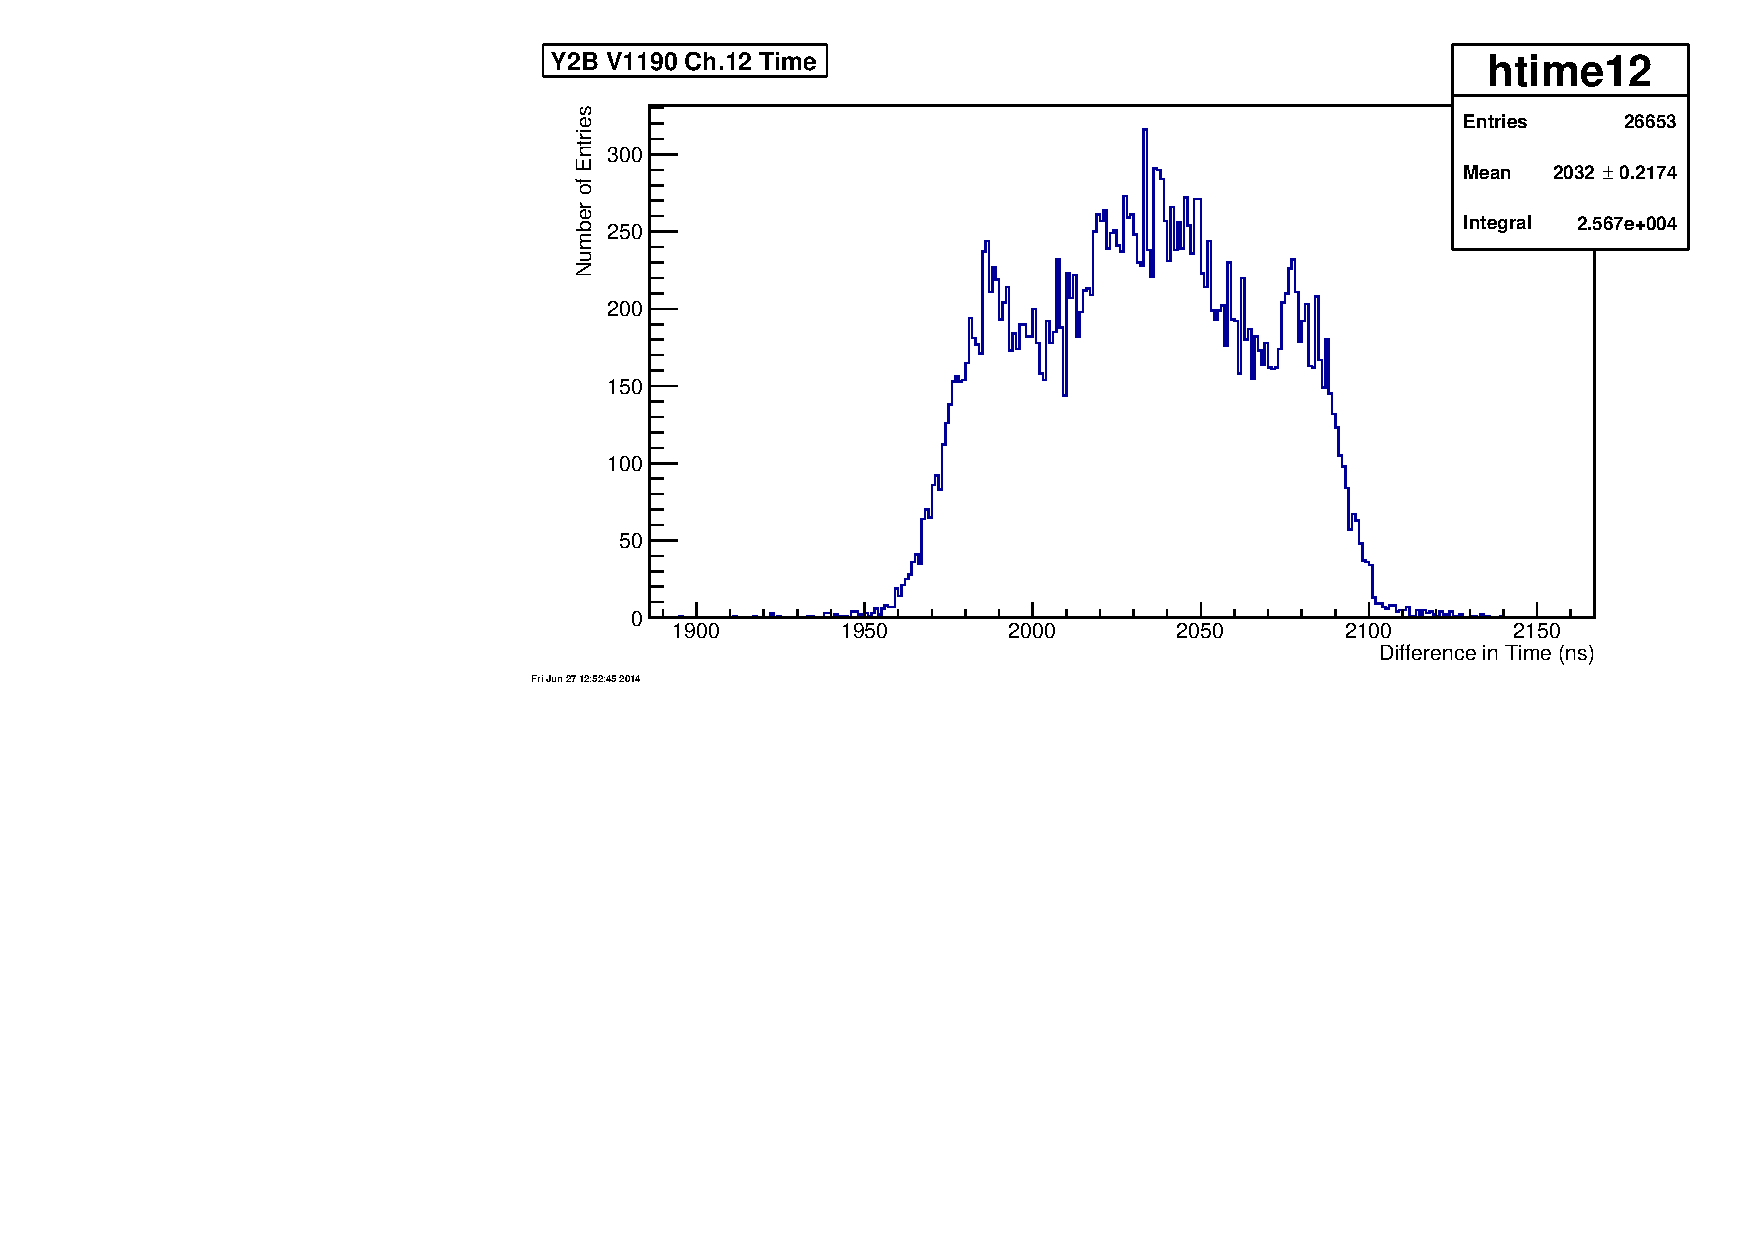
\includegraphics[width=\columnwidth]{run00480_htime12}%
\caption{Raw (uncalibrated) timing spectrum for cathode position signal Y2B.  The range of the timing signal is approximately 150\,ns.  This corresponds to a detector area of 60\,mm, indicating that some of the events are detected outside of the 54\,mm-wide fudicial area of the detector.}%
\label{htime}%
\end{figure}

%\ldots it was suggested that using two detectors may allow ray-tracing of the incident particles.  
\section{In-beam Testing}
\subsection{Beam Time}
\subsubsection{2014 Test}
The beam tests for the EMMA PGAC took place from \longusdate\formatdate{25}{4}{2014} to \longusdate\formatdate{28}{4}{2014} with a total of 35.1\,hours of beam on target.  Data runs were recorded during the day, starting %at 12:53
 on \longusdate\formatdate{26}{4}{2014}. The tests used a beam of $^{16}$O at an energy of 1.103\,MeV$/u$ in a 3+ charge state.  A a 251\,$\mu$g/cm$^2$ gold target was used for the duration of the experiment.  The target is shown in Fig.~\ref{target}.  The target wheel was suspended from the lid of the scattering chamber.  The target being used was in the lower position.  After the experiment, the target appeared to have a burn mark on it.  The PGAC was installed on the HEBT beam line in the ISAC-I experimental hall as shown in Fig.~\ref{schematic}.

\begin{figure}%
\centering
\hspace{\fill}
\includegraphics[width=0.32\columnwidth,height=0.21\textheight,keepaspectratio]{IMG_3221dcR}\hspace{\fill}
\includegraphics[width=0.66\columnwidth,height=0.21\textheight,keepaspectratio]{IMG_3223_21}\hspace{\fill}
\caption{The 251\,$\mu$g/cm$^2$ gold target foil used for the duration of the experiment.  (Left) The target foil as seen by the beam.  (Right) The target foil, viewed downstream, as mounted on the target wheel.  Photos by A.\ Rojas.}%
\label{target}%
\end{figure}
Point of information: The incident beam energy of 1.103\,MeV$/u$ corresponds to a beam particle velocity of 14.58\,mm/ns.  After passing through the gold foil and the 2\,$\mu$m Mylar foil, the energy of the $^{16}$O beam particles is approximately 0.90\,MeV$/u$; corresponding to a velocity of 13.2\,mm/ns.  At this velocity, the transit time of the beam particles between the anodes is approximately 2.8\,ns.

\subsubsection{2015 Test}
The second in-beam test of the PGAC detector took place from \longusdate\formatdate{21}{4}{2015} to \longusdate\formatdate{23}{4}{2015}. A beam of $^{22}$Ne in the $4^+$ charge state was delivered with a nominal beam intensity of 8.5--22.4\,enA (2.1--5.6\,pnA) as measured on \texttt{HEBT:FC14}. A collimator was installed on the target wheel, however the target wheel adjustment mechanism did not have sufficient reproducibility. Therefore,  the 251\,$\mu$g/cm$^2$ gold foil used in the previous test was aligned to the beam axis using a theodolite and left in place for the duration of the experiment. The beam current was then monitored on \texttt{HEBT:FC19} at the end of the beam line. Note: the gold foil was accidentally destoyed during venting.


\subsection{Detector Configuration}
\begin{figure}
\centering
\hspace{\fill}
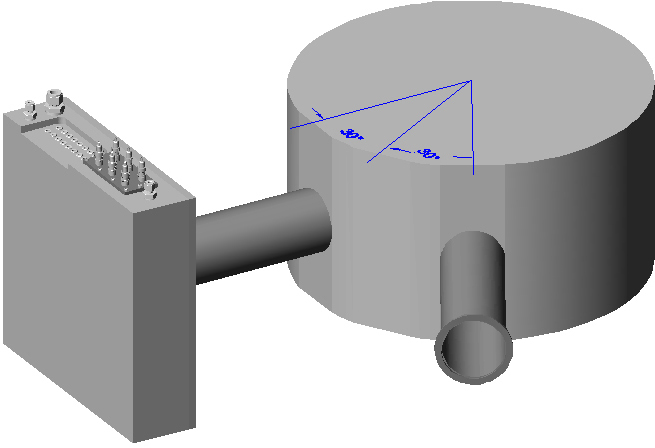
\includegraphics[width=0.48\textwidth,keepaspectratio]{HEBT_Scat_Chamber_3D_trim}\hspace{\fill}
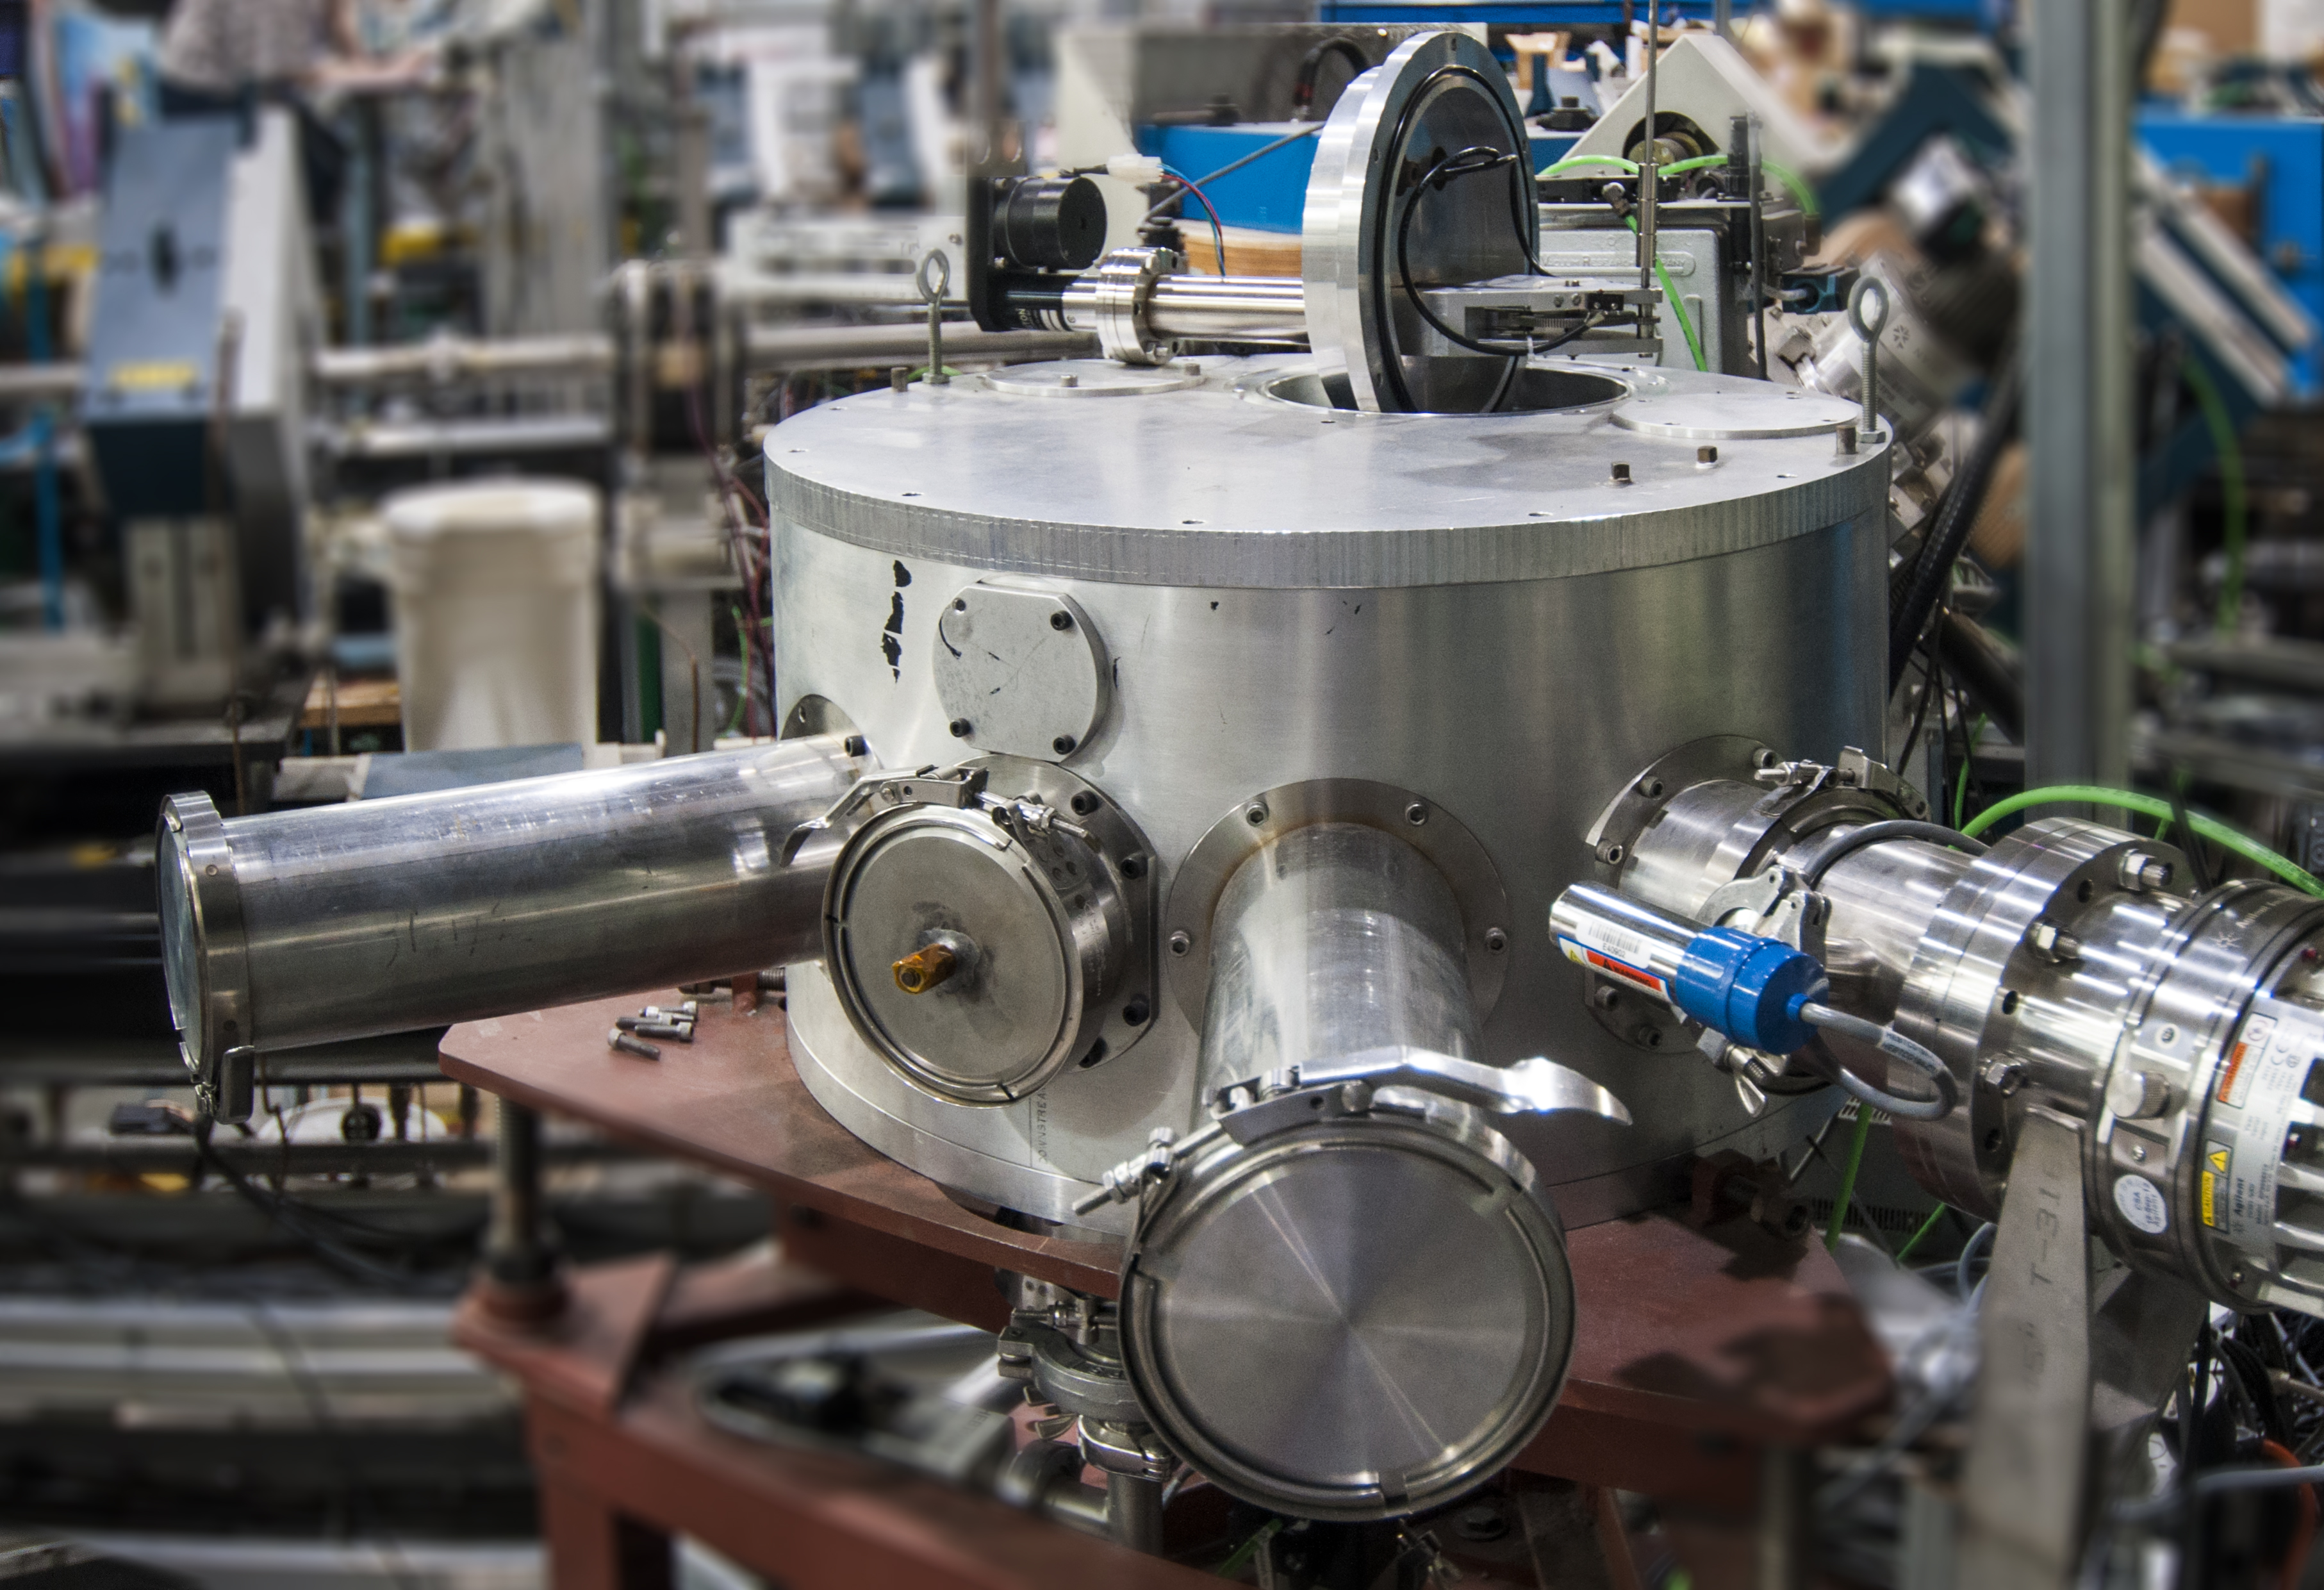
\includegraphics[width=0.48\textwidth, keepaspectratio]{DSC_0004} \hspace{\fill}
\caption{(Left) Schematic diagram of the experimental setup showing a view from downstream of the HEBT beam line.  The beam enters the 0$^\circ$ scattering chamber from the top of the figure.  The beam will bombard a target foil at the center of the chamber and scattering into the PGAC box, mounted at 30$^\circ$ relative to the beam line.  The length of the beam pipe connecting the PGAC box to the scattering chamber is such that 60\% of the active area of the PGAC will be illuminated.  (Right) A photograph of the 0$^\circ$ scattering chamber before PGAC box installation.}
\label{schematic}
\end{figure}
\subsubsection{Settings}
\paragraph{ }The PGAC was tested at four different pressures of %filled with
 isobutane---% 
 %at a pressures of 
 2, 3, 4 and 6\,Torr---%at various points
 during the experiment. The 12.6\,L internal gas volume of the PGAC box was separated from the vacuum of the 50\,L scattering chamber by a 2\,$\mu$m thick Mylar window. The maximum stable voltage was selected for each run, depending on the beam current and the gas pressure. The cathode voltage was varied from $-74$\,V to $-90$\,V and the anode voltage was varied from $+375$\,V to $+490$\,V.  The higher potential differences generally correspond to the higher pressures and the lower potential differences generally correspond to the lower pressures.
 \paragraph{2015 Test} The optimal voltage settings from the first test were used for the second test. The detectors were tested at three different pressures: 2, 3, and 4\,Torr. Low-rate tests at $10\times$ attenuation were  performed on the second and third days. A high-rate test with $17.7\times$ more beam current was also performed on the third day.
\subsubsection{Geometry}
The PGAC box was mounted to the scattering chamber at the end of the HEBT beam line at an angle of 30$^\circ$ relative to the beam line.  Fig.~\ref{schematic} includes a diagram of the experimental setup and a photograph of the scattering chamber. The PGAC was connected to the scattering chamber by a short beam pipe.  The length of the pipe was such that the plane of the %active area
anode of the first PGAC was 682.9\,mm from the target, as shown in Fig.~\ref{rays}.  With the center of the detector located at $\theta_\textrm{lab}=30^\circ$ relative to the beam.  This central trajectory corresponds to $\theta_\textrm{cm}=32.33^\circ$.

\begin{figure}
\centering
\includegraphics[width=\textwidth,keepaspectratio]{EMMA_Test_Stack_Scat_Cham}
\caption{(zoomable online) Orientation of the PGAC box relative to the HEBT scattering chamber. The relative positions of the mask and shield features are listed in Tables~\ref{zpos}, \ref{xpos}, and \ref{ypos}.}
\label{rays}
\end{figure}

The beam pipe shown in Fig.~\ref{rays} defines the minimum scattering angle illuminating the detectors $\theta_\textrm{lab}=30-4.47^\circ=25.5^\circ$ or $\theta_\textrm{cm}=27.5^\circ$.
The maximum scattering angle for each detector is defined by the %angular 
location of the edge of the Kapton shields, the angular position of which varies slightly for each detector.  For detector 2, the maximum scattering angle is $\theta_\textrm{lab}=33.0^\circ$ ($\theta_\textrm{cm}=35.6^\circ$); 89.5\,mm illuminated in the $x$-direction. For detector 1, the maximum scattering angle is $\theta_\textrm{lab}=32.9^\circ$ ($\theta_\textrm{cm}=35.4^\circ$); 92.3\,mm illuminated.
Fig.~\ref{rays} shows that the position of the frame of the Mylar window is in the same angular position as the rearmost Kapton shield for detector one. The alignment of the window frame may also define the maximum scattering angle.
%Therefore, 
Each detector covers about $\Delta \theta_\textrm{lab}=7.4^\circ$, subtending about 10.5\,msr in the laboratory.  The details of these calculations are discussed in Section~\ref{cal_def}.
\subsubsection{Rate}
Given an ion drift time in the PGAC of about 2\,$\mu$s, the desired maximum count rate in the detector was 250\,kHz.
\paragraph{2014 Test}The original beam request assumed that the entire fiducial area of the detector would be illuminated.  Therefore, given the Rutherford scattering cross section of the $^{16}$O beam from the gold foil target, this count rate corresponded to a beam rate of $3.9 \times 10^{10}$\,pps or 6.2\,pnA. During the experiment, three different beam attenuator settings were used.  For most of the experiment, the beam attenuator was set to $10\times$ with an average beam current on-target of 5.05\,enA. Four data runs used the $120\times$ attenuator setting (0.61\,enA) to test the low-count-rate performance of the detector. One data run used the $1\times$ ``attenuator'' (34.0\,enA) to test the high-count-rate performance of the detector.
\paragraph{2015 Test}
The nominal beam current was different each day. The nominal beam current for the three days of the experiment were as follows: 8.8\,enA on the first day, Tuesday, April 21, 2015; 12.7\,enA on the seconday; and  21.3\,enA on the third day.

\subsubsection{Mask}
A different mask was used during each of the in-beam experiments. They are shown in Fig.~\ref{mask} and Fig.~\ref{mask2}. The original mask featured a grid of 5\,mm wide strips. This mask provided a left-right orientation for the $x$-position signals however, it was not suitable for assessing the position resolution of the detector.
A new mask was developed for the 2015 tests featuring a 4.0\,mm $\times$ 4.0\,mm grid of 0.5\,mm holes. This mask allowed for the assessment of the position resolution of the detectors and the linearity of the position.

\begin{figure}
\centering
\includegraphics[width=\textwidth, keepaspectratio]{EMMA_Beam_Test_Mask_with_Kapton_v6.pdf}
\caption{Schematic diagram of the stainless steel mask used during the April 2014 in-beam tests. Dimensions are given relative to the Kapton shield.  The circular opening in the mask was coaxially aligned with the beam pipe and thus the beam.  The relative positions of the mask and shield features are listed in Tables~\ref{xpos} and \ref{ypos}.}%
\label{mask}%
\end{figure}

\begin{figure}[t]
\centering
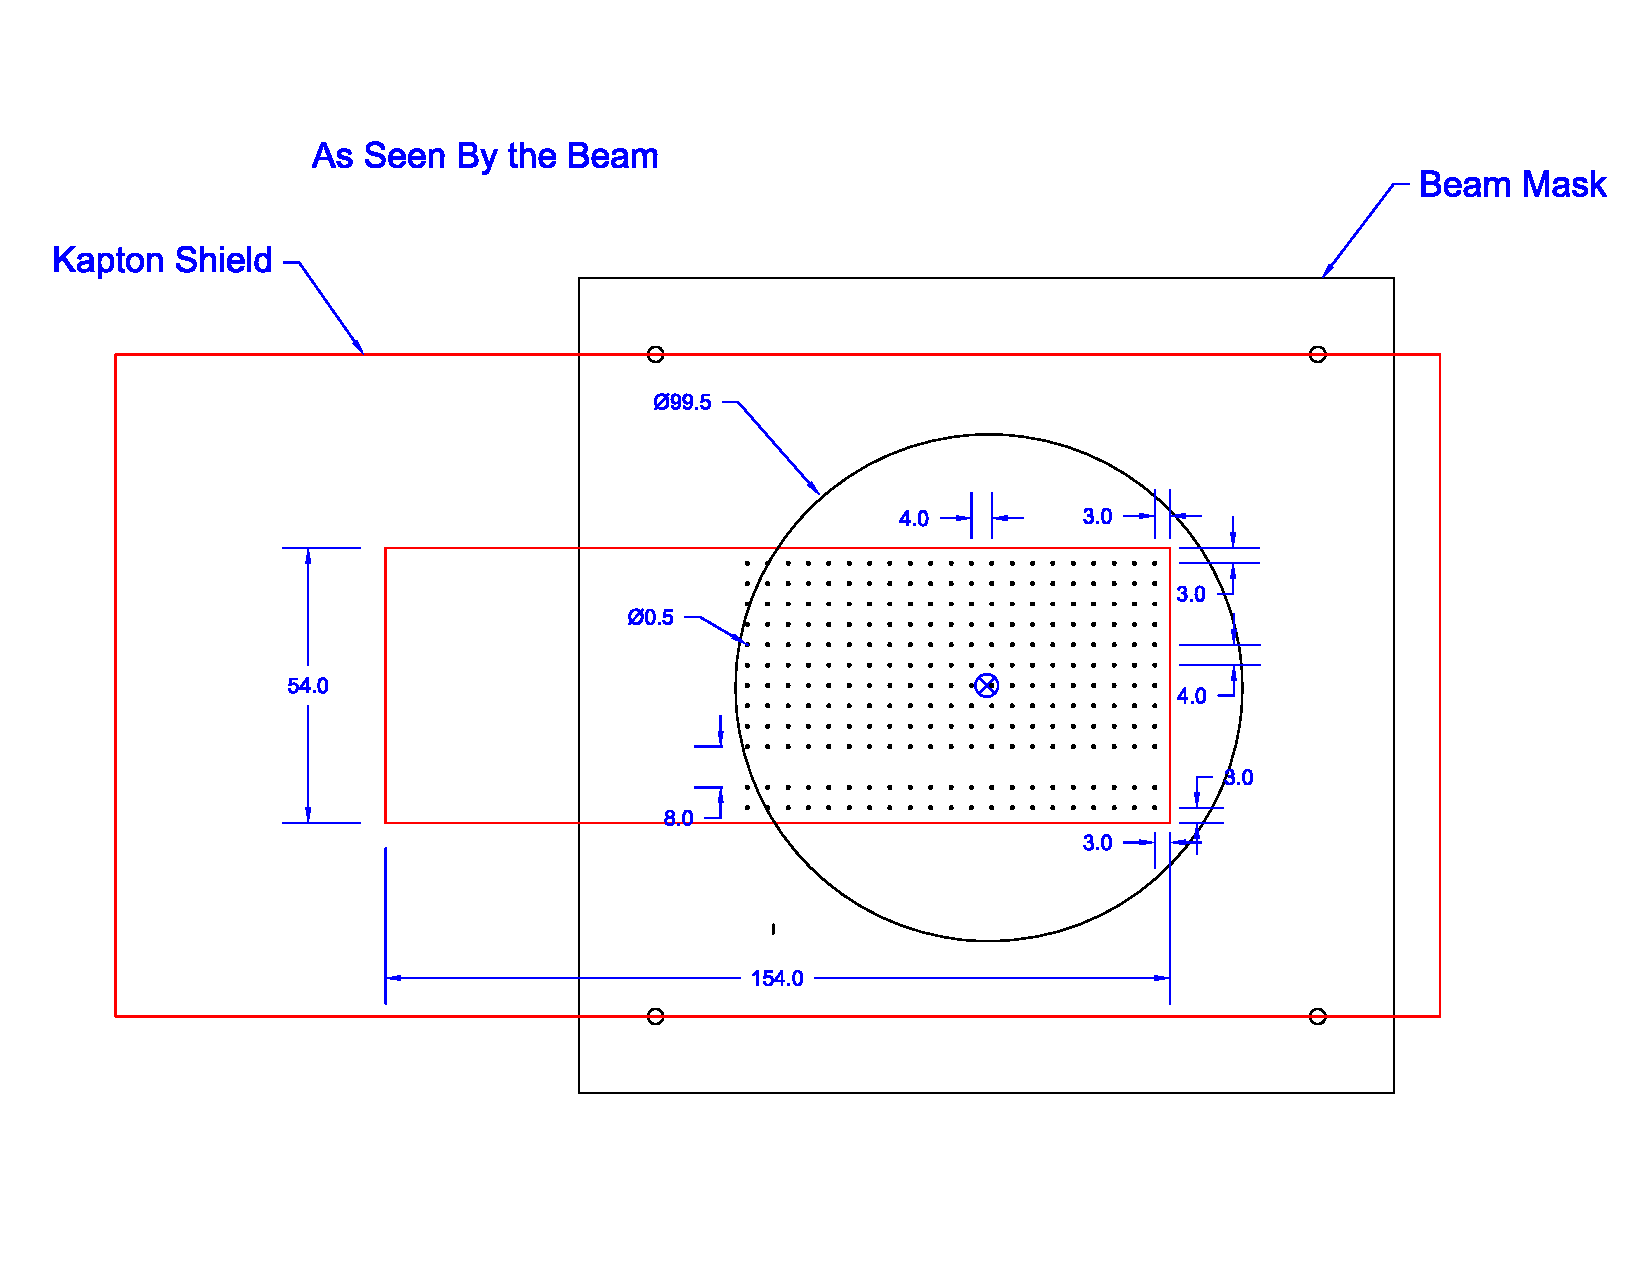
\includegraphics[width=\textwidth, keepaspectratio]{EMMA_Beam_Test_Hole_Mask_2}
\caption{Schematic diagram of the stainless steel mask used during the April 2015 in-beam tests. A 4\,mm lattice of holes was used. Dimensions are given relative to the Kapton shield.  The large circle indicates the diameter of the beam pipe.  The relative positions of the mask and shield features are listed in Table~\ref{xpos2}.
The position of the beam spot is the same as that given in Fig.~\ref{mask}.}%
\label{mask2}%
\end{figure}

\subsection{Electronics Configuration}
The electronics setup is illustrated schematically in Fig.~\ref{e-diagram}.
\begin{figure}[p]
\centering
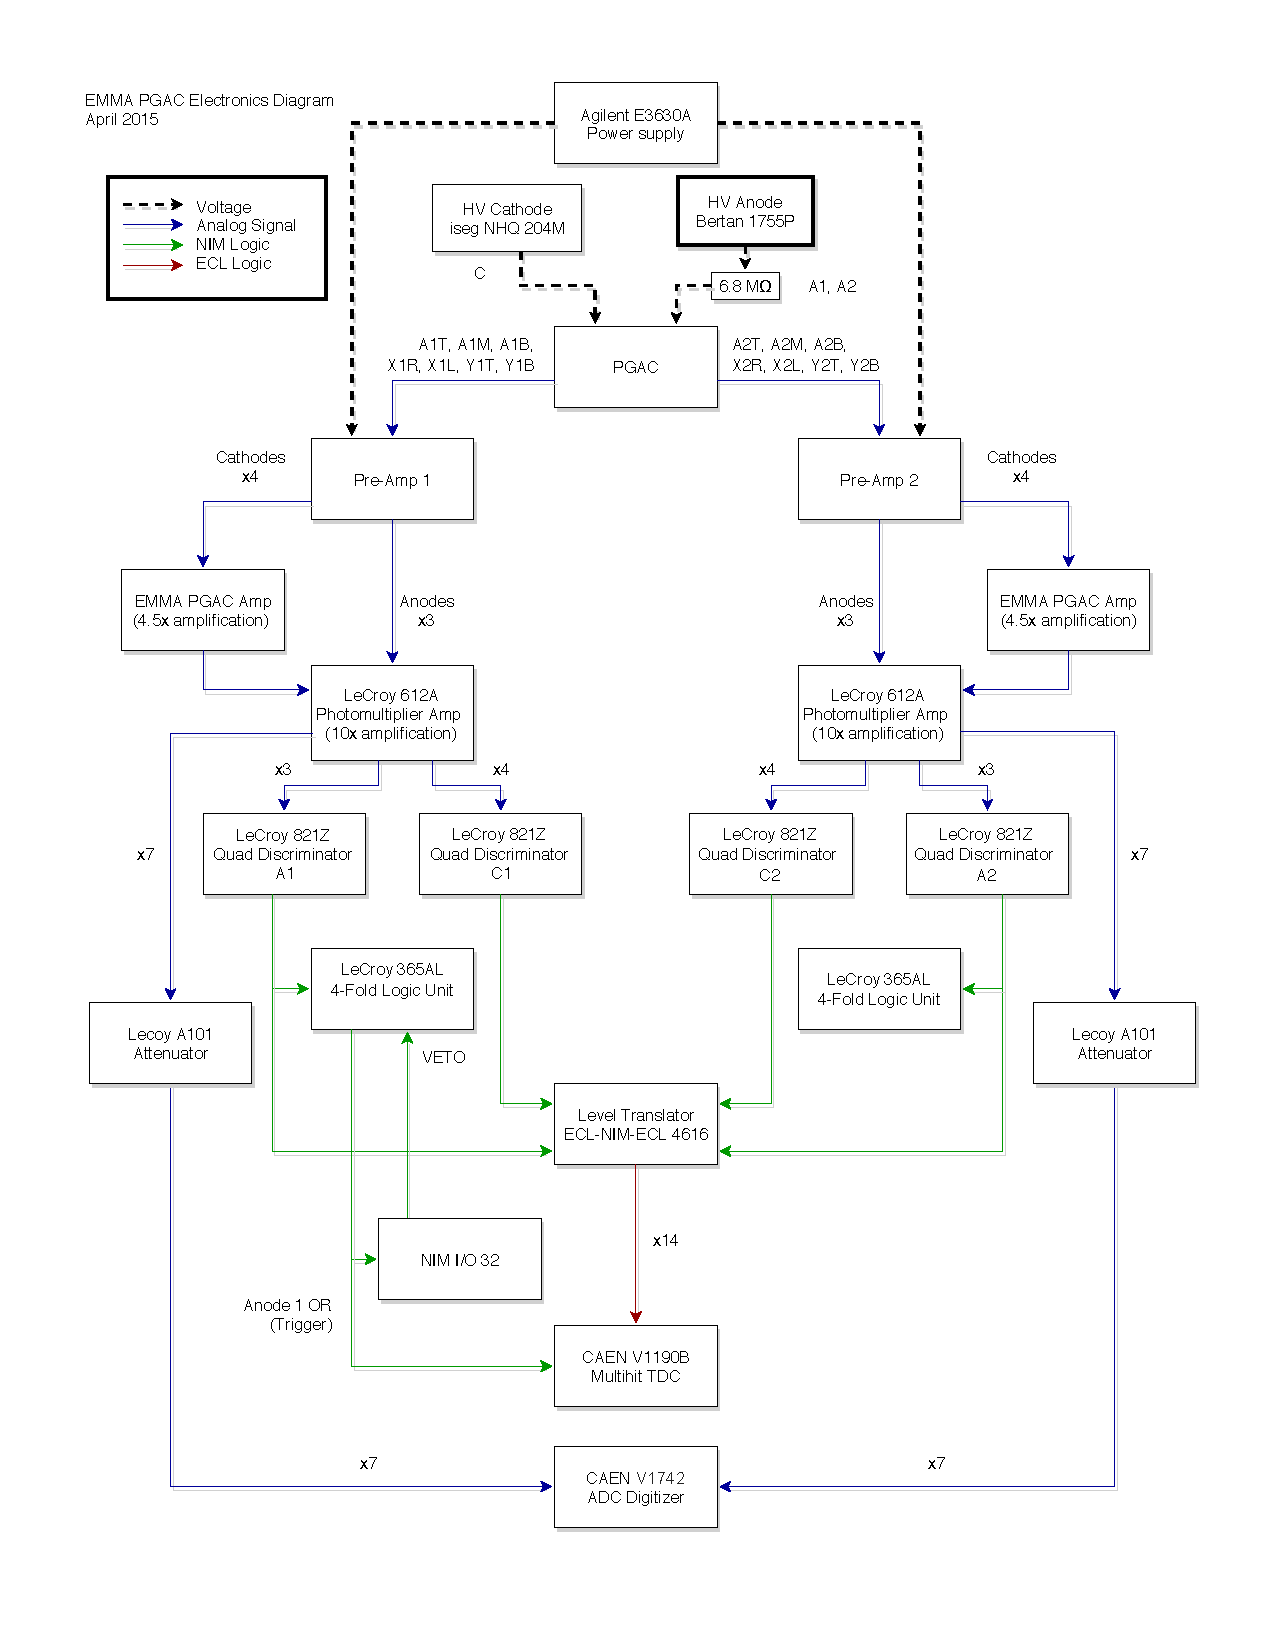
\includegraphics[width=\textwidth, keepaspectratio]{electronics_diagram}
\caption{Electronics diagram for the PGAC tests. Each signal is amplified and passed through a level discriminator to generate a logic signal. The logic signals are read in by the TDC. The logical OR of the anode signals us used to generate the acquisition trigger. A copy of each amplified signal is passed through an attenuator and read in by the waveform digitizer. Drawn by C.\ Ward and R.\ Baker-French.}%
\label{e-diagram}%
\end{figure}
The settings for the TDC, ADC, and pulser were set in MIDAS following the beginning of each run. These settings, in addition to the start and stop time for each run, were recorded in the file \texttt{midas.log} located in  the directory 
\verb|/home/emma/online/| on the LADD cluster. Currently the \texttt{midas.log} file is over 25\,MB in size due to large number of error messages. Removing these lines\footnote{Lines can be removed in emacs using the command \texttt{M-x delete-matching-lines} or \texttt{M-x delete-non-matching-lines}.} reduces the file size to less than 400\,kB.
%\begin{changemargin}{-1in}
%\pangram{100}  
%\end{changemargin}
\subsubsection{Amplifiers}
\label{amp-settings}
All seven signals from each PGAC detector were passed through pre-amplifiers mounted to the PGAC box.  These pre-amplifers were custom built by the Detector Group.  The pre-amp signals were then further amplified using linear fast timing amplifiers.  Two different amplifiers were used: custom-built amplifiers providing approximately 4.5$\times$ amplification and standard %LeCroy xxx 
NIM modules, which provide approximately 10$\times$ amplification. Initially, during the beginning of the data runs, the anode signals were un-amplified and the cathode signals were amplified only  with the the custom-built amplifiers.

The discriminators being used had a minimum threshold setting of 30\,mV and sufficiently low discrimination thresholds were not possible with this configuration. Starting with Run 437, an additional $10\times$ amplification step was added to all of the signals. The added amplification allowed the discriminator thresholds to be set appropriately low. The added amplification step allowed the ratio of the signal peak height to the discriminator threshold level to be reduced by an average factor of $6.5\times$ for the anodes, which produce the trigger. The various discriminator settings are shown in Table~\ref{amp_1_step}.
%
%\begin{figure}
%\centering
%%\includegraphics[width=\textwidth, keepaspectratio]{}
%\textit{<figure to follow>}
%\caption{Electronics diagram.}%
%\label{e-diagram}%
%\end{figure}
\renewcommand{\tabcolsep}{2pt}
\begin{table}[ht!]
\begin{changemargin}{-0em}
\centering  
\hspace{\fill}
\begin{tabular}{c.....}
\hline
\multicolumn{1}{c}{Signal} & \multicolumn{1}{c}{PA}& \multicolumn{1}{c}{Disc} & \multicolumn{1}{c}{Amp} & \multicolumn{1}{c}{Thresh} &\multicolumn{1}{c}{Ratio}\\
&\multicolumn{1}{c}{mV} & \multicolumn{1}{c}{mV}&& \multicolumn{1}{c}{mV} & \textrm{}  \\ \hline \hline
\texttt{A1B} & 112.3 & 112.3 & 1.00 & 30.10 & 0.268 \\
\texttt{A1M} & 120.2 & 120.2 & 1.00 & 30.10 & 0.250 \\
\texttt{A1T} & 122.8 & 122.8 & 1.00 & 30.20 & 0.246 \\
\texttt{A2B} & 135.5 & 135.5 & 1.00 & 60.70 & 0.448 \\
\texttt{A2M} & 124.5 & 124.5 & 1.00 & 30.00 & 0.241 \\
\texttt{A2T} & 130.2 & 130.2 & 1.00 & 29.90 & 0.230 \\
\texttt{X1L} & 37.2 & 179.8 & 4.83 & 30.00 & 0.167 \\
\texttt{X1R} & 34.6 & 157.7 & 4.56 & 30.00 & 0.190 \\
\texttt{Y1B} & 40.5 & 180.9 & 4.47 & 30.00 & 0.166 \\
\texttt{Y1T} & 37.1 & 167.6 & 4.52 & 30.20 & 0.180 \\
\texttt{X2L} & 39.9 & 172.3 & 4.32 & 30.20 & 0.175 \\
\texttt{X2R} & 38.8 & 178.0 & 4.59 & 30.00 & 0.169 \\
\texttt{Y2B} & 42.0 & 190.8 & 4.54 & 30.40 & 0.159 \\
\texttt{Y2T} & 43.2 & 191.6 & 4.44 & 30.00 & 0.157 \\
\hline 
\end{tabular}
\hspace{\fill} \begin{tabular}{c.....}
\hline
\multicolumn{1}{c}{Signal} & \multicolumn{1}{c}{PA}& \multicolumn{1}{c}{Disc} & \multicolumn{1}{c}{Amp} & \multicolumn{1}{c}{Thresh} &\multicolumn{1}{c}{Ratio}\\
&\multicolumn{1}{c}{mV} & \multicolumn{1}{c}{mV}&& \multicolumn{1}{c}{mV} & \textrm{}  \\ \hline \hline
\texttt{A1B} & 127.0 & 1100.0 & 8.66 & 55.00 & 0.050 \\
\texttt{A1M} & 123.0 & 1170.0 & 9.51 & 60.00 & 0.051 \\
\texttt{A1T} & 120.0 & 1130.0 & 9.42 & 65.00 & 0.058 \\
\texttt{A2B} & 137.0 & 1510.0 & 11.02 & 55.00 & 0.036 \\
\texttt{A2M} & 126.0 & 1420.0 & 11.27 & 56.00 & 0.039 \\
\texttt{A2T} & 131.0 & 1520.0 & 11.60 & 57.00 & 0.038 \\
\texttt{X1L} & 36.0 & 1670.0 & 46.39 & 58.00 & 0.035 \\
\texttt{X1R} & 34.0 & 1650.0 & 48.53 & 200.00 & 0.121 \\
\texttt{Y1B} & 41.0 & 1850.0 & 45.12 & 210.00 & 0.114 \\
\texttt{Y1T} & 39.0 & 1740.0 & 44.62 & 200.00 & 0.115 \\
\texttt{X2L} & 40.0 & 1850.0 & 46.25 & 200.00 & 0.108 \\
\texttt{X2R} & 40.0 & 1800.0 & 45.00 & 200.00 & 0.111 \\
\texttt{Y2B} & 44.0 & 1960.0 & 44.55 & 200.00 & 0.102 \\
\texttt{Y2T} & 43.0 & 1910.0 & 44.42 & 200.00 & 0.105 \\
\hline 
\end{tabular}
\hspace{\fill}
\caption{Discriminator values before and after the inclusion of an extra $10\times$ amplification. The signal level at the output of the preamplifier (PA) and at the input of the discriminator (Disc) is given. The ratio of these two values gives the amount of amplification applied to the signal (Amp). The discriminator threshold (Thresh) is also given. The minimum discriminator threshold was 30\,mV. Finally, the ratio of the discriminator threshold to the discriminator input signal is given. For both amplification settings, the detector had the following settings $P=3$\,Torr, $V_\textrm{a}=410$\,V, $V_\textrm{c}=-75$\,V, $\Delta V=485$\,V. }
\label{amp_1_step}
\end{changemargin}
\end{table}
\renewcommand{\tabcolsep}{6pt}%\the\tabcolsep

\subsubsection{TDC}The detector signals were read into the acquisition system using two different methods.  The first method used a time-to-digital converter (TDC), specifically a CAEN V1190B-2eSST 64 Channel Multihit TDC module.  The TDC has a full range of 4,0$96 \times 10$ channels and was configured for 200\,ps per channel. The TDC measures the arrival time of logic pulses relative to a trigger pulse.   The amplified signals from the PGAC were entered into leading-edge discriminators to produce the logic signals required by the TDC.  The logical OR of the anode signals of detector 2 (the detector facing the beam) was used to generate the trigger.
\begin{table}%

\begin{minipage}{\textwidth}
\begin{center}
  

%
%
\begin{tabular}{rrr|rrcc|cc}
%\multicolumn{1}{c}{Plane} & \multicolumn{1}{c}{$z$-position} \\ 
\hline
%\multicolumn{1}{c}{TDC\footnote{April 2014}} & \multicolumn{1}{c}{TDC\footnote{April 2015}} &

\multicolumn{2}{c}{TDC} & %\multicolumn{1}{c}{TDC} &

\multicolumn{1}{c}{ADC} &\multicolumn{1}{|c}{Label}& \multicolumn{1}{c}{Pair} & Position & Side & Branch & Leaf \\
\cline{1-2} 
\multicolumn{1}{c}{2014} & \multicolumn{1}{c}{2015} & \multicolumn{1}{c}{}\\
\hline \hline
 0 &  0 &  0 &\texttt{A1B} & 0 & bottom & ---&PGAC1&ab\\
 1 &  1 &  1 &\texttt{A1M} & 1 & middle & ---&PGAC1&am\\
 2 &  2 &  2 &\texttt{A1T} & 2 & top & ---&PGAC1&at\\
 3 &  3 &  3 &\texttt{A2B} & 0 & bottom & ---&PGAC2&ab\\
 4 &  4 &  4 &\texttt{A2M} & 1 & middle & ---&PGAC2&am\\
 5 &  5 &  5 &\texttt{A2T} & 2 & top & ---&PGAC2&at\\ \hline 
 6 &  {\color{red}9} &  8 &\texttt{X1L} & 3 & right & far&PGAC1&xf\\
 7 &  {\color{red}8} &  9 &\texttt{X1R} & 3 & left & near&PGAC1&xn\\
 8 &  {\color{red}7} & 10 &\texttt{Y1B} & 4 & bottom & near&PGAC1&yn\\
 9 &  {\color{red}6} & 11 &\texttt{Y1T} & 4 & top & far&PGAC1&yf\\
10 & 10 & 12 &\texttt{X2L} & 5 & right & far&PGAC2&xf\\
11 & 11 & 13 &\texttt{X2R} & 5 & left & near&PGAC2&xn\\
12 & 12 & 14 &\texttt{Y2B} & 6 & bottom & near&PGAC2&yn\\
13 & 13 & 15 &\texttt{Y2T} & 6 & left & far&PGAC2&yf\\
 \hline 
\end{tabular}
\end{center}
\end{minipage}

\caption{Input signals to the TDC and ADC.  Note that in the April 2015 tests, the position signals for detector 1 were plugged in backwards. Note also that the signals input to the ADC are split into two groups: signal inputs 0--5 and inputs 8--15. The 14 signals formed 7 pairs.  The position are given as seen by the beam.  For each position, signals are ``near'' or ``far'' relative to the bottom left corner of the fiducial area of the detector. The branch and leaf names for tree sorting are also given.}
\label{TDC_signals}
%
\end{table}

The detector signals were connected to the TDC in the order shown in Table~\ref{TDC_signals}. Ideally, all 14 signals (7 from each detector) would have been read into the TDC.  In this manner, the signal from each segment of the anode is read in independently.  However, only the logical OR of the anode signal was read into the TDC.  Therefore, each detector had 5 signals associated with it.  The ORs of the anode signals for each detector were read into the channel corresponding to the A$n$M signal.

\subsubsection{Digitizer}Copies of the amplified detector signals were also fed into a waveform digitizer, specifically a CAEN V1742 32+2 Channel 12-bit 5\,GS/s Switched Capacitor Digitizer module. 
The V1742 is based on two DRS4 (%\footnote{DRS4 is an abbreviation of 
Domino Ring Sampling, revision 4) %.}
 chips, each with $16+1$ channels.  %Each channel has a fixed jitter constant that needs to be corrected for during calibration.
Each of the 16+1 channel groups have their own trigger and are further divided into two input signal groups. % These groups  
%The inputs of the V1742 are divided into two different groups, corresponding to signals 0--7 and 8--15.
Each of the two input groups has an independent timing correction. Table~\ref{TDC_signals} shows that the anodes of both detectors were input into the first group and the cathodes were input into the second group.

%\marnote{check}
Of the 69 total data runs, 47 of them had the digitizer enabled.
 The digitizer was operated at 1.0, 2.5, and 5.0\,GS/s.  These sample rates correspond to timing resolutions of 1.00\,ns, 400\,ps, and 200\,ps, respectively.
 Since the V1742 is an analogue digitizer, the memory buffer has a fixed size of 1024 cells. The different sample rates correspond to acquisition windows of 1.024\,$\mu$s, 409.6\,ns, and 204.8\,ns, respectively.
 During most of the runs the digitizer was set to 1.0\,GS/s. For 7 data runs the digitizer was set to 2.5\,GS/s and for 10 data runs it was set to 5.0\,GS/s.  The digitizer settings were written to memory \textit{after} the start of each run and could not be changed during the run. Care must be taken when parsing MIDAS log file to ensure that the digitizer status  is properly associated with the correct run number.
 %written \textit{after} the start of the run is the setting for that run.
 
 The analog input dynamic range of the TCDC is 1\,V peak-to-peak.  Therefore, depending on the detector bias and the amplification, the amplified detector signals needed to be attenuated in order to fit within the 1\,V range of the digitizer.  An array of independently adjustable 50\,$\Omega$ attenuators was used to provide the minimum attenuation required to keep the peak-to-peak signal amplitude under 1\,V.  Typical values of attenuation was 0.5$\times$.
	

\section{Files}
\subsection{Data}
\sloppy
\subsubsection{Location}
The data from this experiment was saved in the directory 
\verb|/ladd/data2/emma/data/| on the LADD cluster.  The data is physically located on the computer \texttt{ladd02.triumf.ca}. Assuming \texttt{ladd02} is turned on and connected to the network, the data is accessible with the \texttt{emma} user account on any of the LADD cluster servers, such as \texttt{ladd19}, \texttt{ladd20}, or \texttt{ladd21}. The data has been copied to the computer \texttt{lighthall.triumf.ca} and is located in the directory \verb|/Users/lighthall/data/PGAC_test/data|.
A symbolic link to the data directory has been made in the analysis directory with the name \verb|data\|.
\subsubsection{Accessing the data}
The LADD cluster does not use individual usernames. Each group is assigned group login credentials. The login credentials for the EMMA group are given below.
\begin{quote}
\interlinepenalty=1000
  \begin{verbatim}
    username: emma
    password: daq_test2014
  \end{verbatim}
\end{quote}
\vsetlinux
Log onto the LADD cluster using SSH via the servers \texttt{ladd19}, \texttt{ladd20}, or \texttt{ladd21}.  If connecting from offsite,  \texttt{.trifumf.ca} must be appended to the server address. The command for logging onto the cluster follows.
\begin{quote}
  \begin{Verbatim}
ssh -Y emma@ladd19.triumf.ca 
		\end{Verbatim}
\end{quote}
In this example, the \texttt{ladd19} computer is used. The \texttt{-Y} flag is used to enable X11 tunneling in order to view histograms, etc. on the remote computer. In order to view windows on the remote computer, make sure an X Windows program is running on the local computer, for example XQuartz (OS X) or XWin (Windows). After entering this command, you will be prompted for the EMMA account password. Once logged in, the user will start out in the EMMA home directory \verb|\home\emma|.
\subsubsection{Run contents}

The April 2014 experiment started with Run 371 and ended on Run 480.  Of these 110 runs, 69 of them were written to disk. 
The settings of the runs are discussed in Section~\ref{settings_sec}.  
Except where indicated otherwise, all of the data referred to in this section is from Run 480.

%, which was the last run of the experiment.
Run 480 was selected---arbitrarily---because it was the last run of the experiment. The data for this run is contained in five MIDAS files. The duration of the run was 13\,min 25\,sec. After sorting, this run contains about 30,000 events, with 25,000--29,000 in pair-wise coincidence, depending on signals in question. The detector settings for this run were $P=3$\,Torr, $V_\textrm{c}=-80$\,V, $V_\textrm{a}=+435$\,V ($\Delta V=515$\,V).  The beam current for this run was 0.64\,enA ($120\times$ attenuator). It was one of 17 data runs at $P=3$\,Torr. Because of the low beam intensity, Run 480 had the highest $\Delta V$ setting of any other run at $P=3$\,Torr.  For example, it was the only run at $P=3$\,Torr with $V_\textrm{c}$ set to a value other than $-75$\,V.

The April 2015 experiment started with Run 576 and ended with Run 611. Of the 36 runs, data was written to disk for 24 runs. The initial calibration constants were developed for Run 606. The thresholds of every detector channel were optimized before the start of this run and should represent an optimized electronics setup.

\subsection{Readout}
\vsetlinux
The main analysis program is \texttt{ana.cxx}. Four vairations of the readout code have been developed by the author.
References to readout code in the following sections refer to the program \texttt{ana.cxx} currently located in 
\verb|ladd19.triumf.ca:/home/emma/offline/lighthall/rootana/analysis/|.  Here \texttt{ladd19} 
could be replace with any of the computers in the LADD cluster.  This readout program is built upon the minimum working example readout code located in \verb|ladd19.triumf.ca:/home/emma/packages/rootana/examples/|. The readout programs utilize the \texttt{TV1190Data.hxx} class.

\subsubsection{\texttt{ana\_bare.cxx}}
The file  \texttt{ana\_bare.cxx} is a stripped-down minimal working example (``bare bones'') of the readout code. 
The code is run with the command
\begin{quote}
  \begin{Verbatim}
./ana_bare.exe data/run00606sub00000.mid.gz   
\end{Verbatim}
\end{quote}
and output files are saved into the directory \verb|./output/| with the file name \verb|emma_ana_bare_00606.root|.


The structure of the code discussed here applies to the three other readout codes.
The program contains two main functions which are modified for the purposes of calibration and analysis.
At the start of each run, the function \verb|BeginRun()| is called. This code is run once per data set. Here the histograms are defined.

The data are read out using the function \texttt{ProcessMidasEvent()} within the \texttt{TRootanaEventLoop} class. This function is called once per event.
The data are first parsed into channel number and value using the TV1190Data class.   
Once the data is unpacked by \texttt{ProcessMidasEvent}, they are filled into ROOT histograms. 
A number of ``raw'' histogram are filled with uncalibrated data. This is illustrated in the following code box. %\newpage
%\pangram{50}%\hline
\vspace{0.5\baselineskip}
\par\noindent
\begin{minipage}{\linewidth}
  \singlespace
\begin{lstlisting}[caption={Unpack data. Here for a given event, \texttt{chan} is a variable which takes the value of the channel number, %for which an event has been recorded,
 \texttt{counts} records the number hits per channel , \texttt{datum} is an array which stores all of the measurements for a given event,
 and \texttt{hdata} is a raw histogram of counts per channel. }]
//--- Unpack data
for(unsigned int i = 0; i < measurements.size(); i++) { //loop over measurements
   chan = measurements[i].GetChannel();
   counts[chan]++; //"counts" per channel (multi-hit)
   datum[chan][counts[chan]] = measurements[i].GetMeasurement();
   hdata[chan]->Fill(datum[chan][counts[chan]]);//raw data histograms
}
\end{lstlisting}
%\vspace{-1.3\baselineskip}
\end{minipage}


\subsubsection{\texttt{ana.cxx}}
The file  \texttt{ana\_bare.cxx} is a stripped-down minimal working example (``bare bones'') of the readout code. 
The code is run with the command
\begin{quote}
  \begin{Verbatim}
./ana.exe data/run00606sub00000.mid.gz   
\end{Verbatim}
\end{quote}
and output files are saved into the directory \verb|./output/| with the file name \verb|emma_ana_00606.root|.
%the function \verb|BeginRun()| and 
Calibration parameters are read in with a simple file I/O subroutine. The calibration constants are stored in text files located in the directory
\verb|ladd19.triumf.ca:/home/emma/offline/lighthall/rootana/analysis/cal/|. Default calibration constants were developed for runs 430, 480, and 606 which were the most thoroughly analyzed runs. In cases where these default values do not properly calibrate the data, additional calibration constants were developed on a run-by-run basis.

%\hline
%\pangram{50}
%Here for a given event, \texttt{chan} is a variable which takes the value of the channel number, %for which an event has been recorded,
% \texttt{counts} records the number hits per channel , \texttt{datum} is an array which stores all of the measurements for a given event,
% and \texttt{hdata} is a raw histogram of counts per channel.
  After the raw histograms are filled, the calibration parameters which were previously read in % from files during the sort routine and
are applied to the data and additional histograms are filled.

\subsubsection{\texttt{anaDisplay.cxx}}
The waveforms are read out using the program \texttt{anaDisplay.cxx}. The online version of this code, which was used during the in-beam tests is located in the directory \verb|ladd19.triumf.ca:/home/emma/packages/rootana/examples/|. The author has continued development in the directory \verb|ladd19.triumf.ca:/home/emma/offline/lighthall/rootana/analysis/|.

Canvases and histograms are defined in the functions \texttt{AddAllCanvases()}, \texttt{BeginRun()}, and \texttt{PlotCanvas}. The data is unpacked in the function \texttt{UpdateHistograms}. Histograms are then filled and no calibrations are applied. The function \texttt{doV1742} handles the unpacking and plotting of digitized waveforms.
The display allows the option for processing a certain number of events before displaying them.  So for instance, to process 5000 events and then display, do
\begin{quote}
  \begin{Verbatim}
./anaDisplay.exe /ladd/data2/emma/data/run00480sub00004.mid.gz -s5000
\end{Verbatim}
\end{quote}
If you just want to process 5000 events and then exit, then you can do
\begin{quote}
  \begin{Verbatim}
./anaDisplay.exe /ladd/data2/emma/data/run00480sub00004.mid.gz -s5001 -e5000
\end{Verbatim}
\end{quote}
The \texttt{-e} flag says 'quit after processing \texttt{XXX} events'; \texttt{-s} flag says 'process \texttt{YYY} events before displaying'. Using the two together is a bit of a kludge (I didn't really intend for people to do that) but it would work for some quick analysis.

\subsubsection{\texttt{ana\_tree.cxx}}
The file \texttt{ana\_tree.cxx} is used to translate MIDAS files into ROOT files containing trees. The creation of raw histograms have been included in this code for reference.
The file  \texttt{ana\_bare.cxx} is a stripped-down minimal working example (``bare bones'') of the readout code. 
The code is run with the command
\begin{quote}
  \begin{Verbatim}
./ana_tree.exe data/run00606sub00000.mid.gz   
\end{Verbatim}
\end{quote}
and output files are saved into the directory \verb|./output_tree/| with the file name \verb|emma_ana_bare_00606.root|.
\subsection{Analysis}
The analysis utilizes developed by the author are located in the directory \verb|/home/emma/offline/lighthall/rootana/analysis/scripts|. By launching ROOT from the parent directory, \verb|/home/emma/offline/lighthall/rootana/analysis/|, the local \texttt{rootlogon.C} is read in which loads the macro packages \texttt{fit.cc} and \verb|load_and_plot.cc|. ROOT is launched from the analysis directory using any of the following commands.

\begin{quote}
\begin{Verbatim}
root -l
root -l output/emma_ana_bare_00606.root
root -l output/emma_ana_00606.root
root -l output_display/emma_anaDisplay_00442.root 
root -l output_tree/emma_ana_00606.root 
\end{Verbatim}
\end{quote}
\vsetnone

The file \texttt{fit.cc} contains many general purpose histogram display and analysis macros which are applicable to most data sets. The file \verb|load_and_plot.cc| mostly contains macros for re-creating specific figures but also includes some macros relevant to the PGAC analysis. Both files are under version control.
\subsubsection{\texttt{fit.cc}}
\label{fit}
Some useful display macros found in \texttt{fit.cc} are as follows.
\paragraph{Display}
\vsetroot
\begin{quote}
\begin{Verbatim}[firstnumber=0]
dr("hdata0")
dr("hxfxn")
dr("htrace")
\end{Verbatim}
\end{quote}
\texttt{dr()} will take a histogram of any type (1D, 2D, etc.) and plot it on the current canvas. If no canvas is open, one will be created.
\begin{quote}
\begin{Verbatim}[firstnumber=0]
plotall("hdata")
\end{Verbatim}
\end{quote}
\texttt{plotall()} will find all histograms with titles matching the value entered, in this example \texttt{"hdata"}. Next, based on the number of histograms found, 14 in this example, the canvas will be divided appropriately ($4\times4$).
\paragraph{Fitting}

There are three peakfitting routines. \texttt{peakfit()} operates on a 1D spectrum and \texttt{peakfitx()} and \texttt{peakfity()} create $x$- and $y$-projections, respectively, of a given 2D histogram. The peakfit routines determine the positions of the peaks in the spectrum in three steps. First, the peaks are found in the spectrum using the \texttt{Search} function in the \texttt{TSpectrum} class built in to ROOT. This is performed in the subroutine \texttt{findpeaks()}.The number of peaks are found and are output in order of peak height. Using this routine, peaks are found bin-wise and the center of each peak is given as the center of a given bin. Therefore, calibrations based on these positions alone will always have an error based on the intrinsic offset between the true peak center and the reported center, which always corresponds to the center of a bin.

In order to derive the center of the peaks, each peak must be fit with a Gaussian function (or other appropriate fit function). The first step in the peak-fitting routine also calculates the minimum separation between peaks. This determines the fit range of the Gaussian fits to provide non-overlapping fits. The second step of the peak-fit routine takes the peak position and peak separation given by \texttt{findpeaks()} and calculates Gaussian fits in non-overlapping regions. This step is carried out by the subroutine \texttt{gfindpeaks()}. For each peak found in \texttt{findpeaks()}, \texttt{gfindpeaks()} outputs three fit parameters, the amplitude, mean $\mu$, and width $\sigma$ of the fit. The peak centers output from this routine are typically good enough to produce linear calibration parameters that rapidly converge. However, if the peaks are closely spaced and information is needed about the number of count attributable to each individual peak, a convoluted fit is required.

The final step of the peak-fitting routine is a global fit with $n$ Gaussian peaks. The $3n$ parameters generated by \texttt{gfindpeaks()} are used as initial conditions for a global fit. This process is carried out by the subroutine \texttt{decon()}, which can handle up to 20 peaks in a given 1D spectrum. After the best fit of the individual peaks has been determined by the global fit, the individual fit parameters are output. The peak centers given by this method should be as close to the true center of the peaks as can be determined.

After the fit parameters have been determined, the individual peak widths and calculated peak areas are plotted as a function of peak center in a new canvas. This is particularly useful for assessing position dependence of resolution and, possibly, efficiency.

\subsubsection{\texttt{load\_and\_plot.cc}}
The code relevant to PGAC analysis starts on line 3330 (in version 761).




\section{Calibration}
The PGAC data is calibrated in three steps. All of the data analysis is derived from time measurements made using the TDC and is therefore based on pairs of detector signals. The first step of the calibration is determining which pairs of signals from the multi-hit TDC go together. Then the appropriate signals need to be gain-matched. Once the detector signals are internally consistent---having been appropriately paired and gain-matched---the position calibration is applied.
\subsection{Multi-hit}
The V1190 TDC can register multiple hits for the same channel within the trigger window. Under normal conditions, each channel only has one hit per trigger event.
Fig.~\ref{mhit} (Right) show the total muliti-hit counts for A2M, the middle anode of detector 2. All events have three or fewer hits per event, with most events only having one hit. This behavior is consistent for the other channels. In about 3\% of trigger events, the TDC registers two hits for the same channel.

 Fig.~\ref{mhit} (Center) shows the data spectrum of A2M with first-hits shown in blue and second-hits shown in red. In this context, ``first hit'' refers to the first memory position read out from the TDC hit register for a given channel. The figure shows that the second-hits appear later in time and are unassociated with the main locus of data. Fig.~\ref{mhit} (Right) shows that these later events are correlated between anodes, but the distribution is about $150\times$ that of the first-hit correlations. The sharply-correlated data corresponds to the first hit, or equivalently, the hit which occurs earliest in time. Therefore multi-hit data selection is based on the hit with the lowest channel number (the ``earliest hit'') registered for each channel, or the first hit read out from the TDC for each channel.

\begin{figure}
\centering
\centerline{
\hspace{\fill}
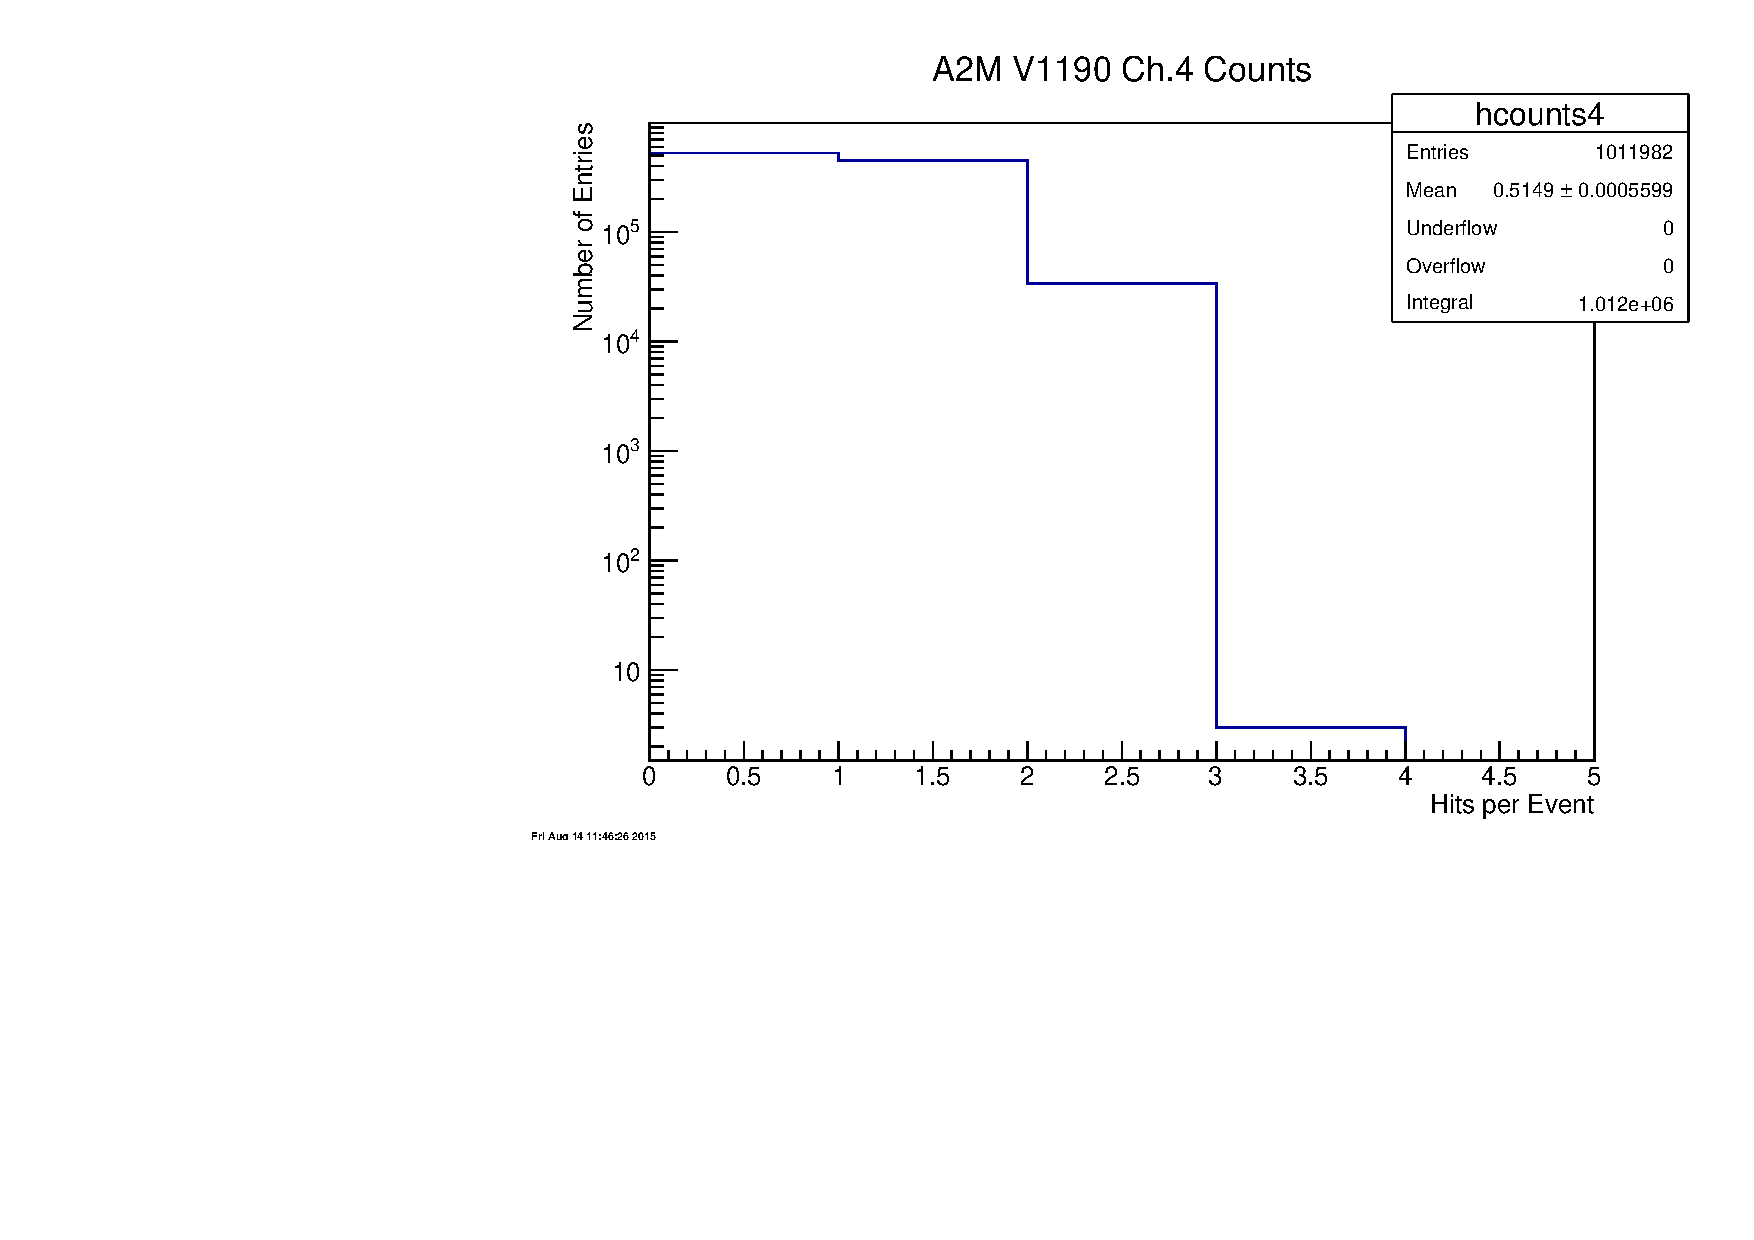
\includegraphics[width=0.4\textwidth,keepaspectratio]{run_606_hcounts4}\hspace{\fill}
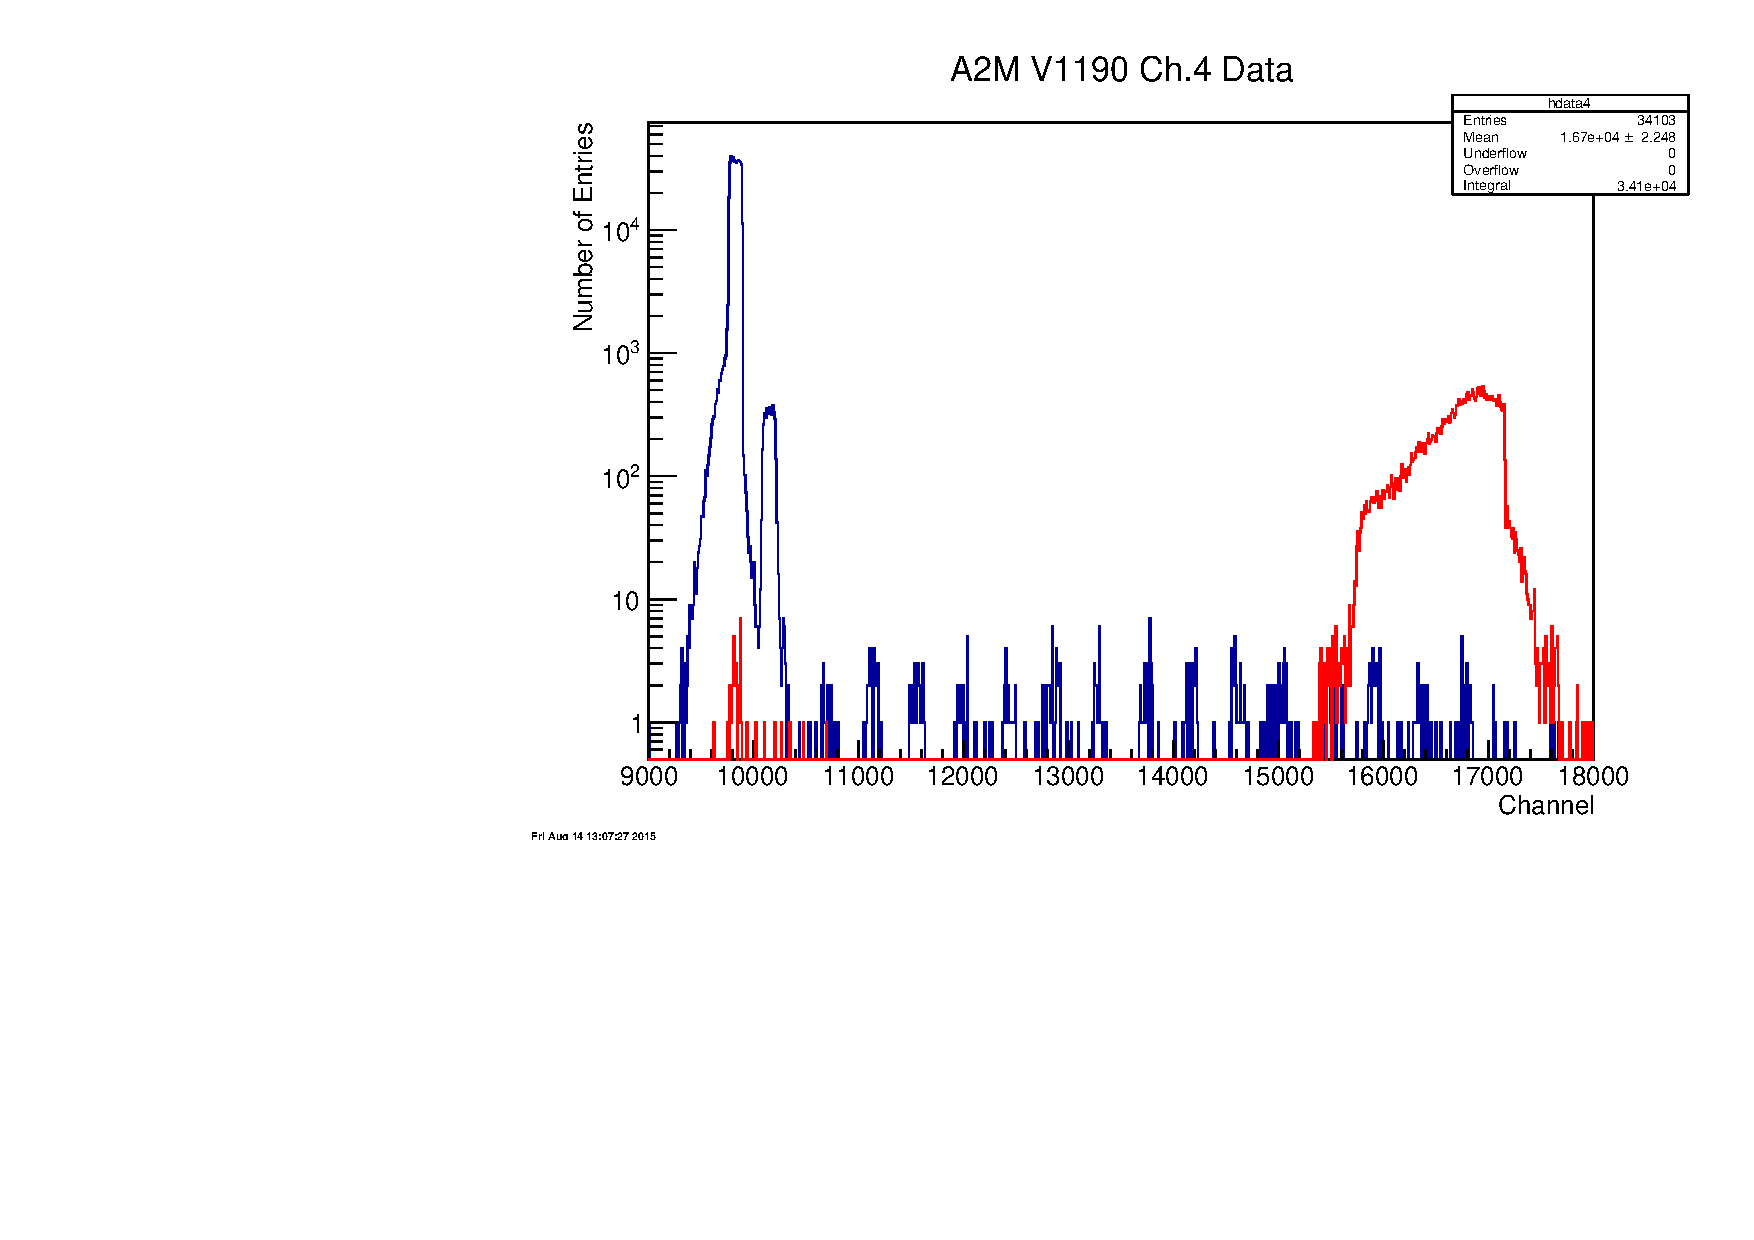
\includegraphics[width=0.4\textwidth,keepaspectratio]{run_606_hdata_1_2_zoom}\hspace{\fill}
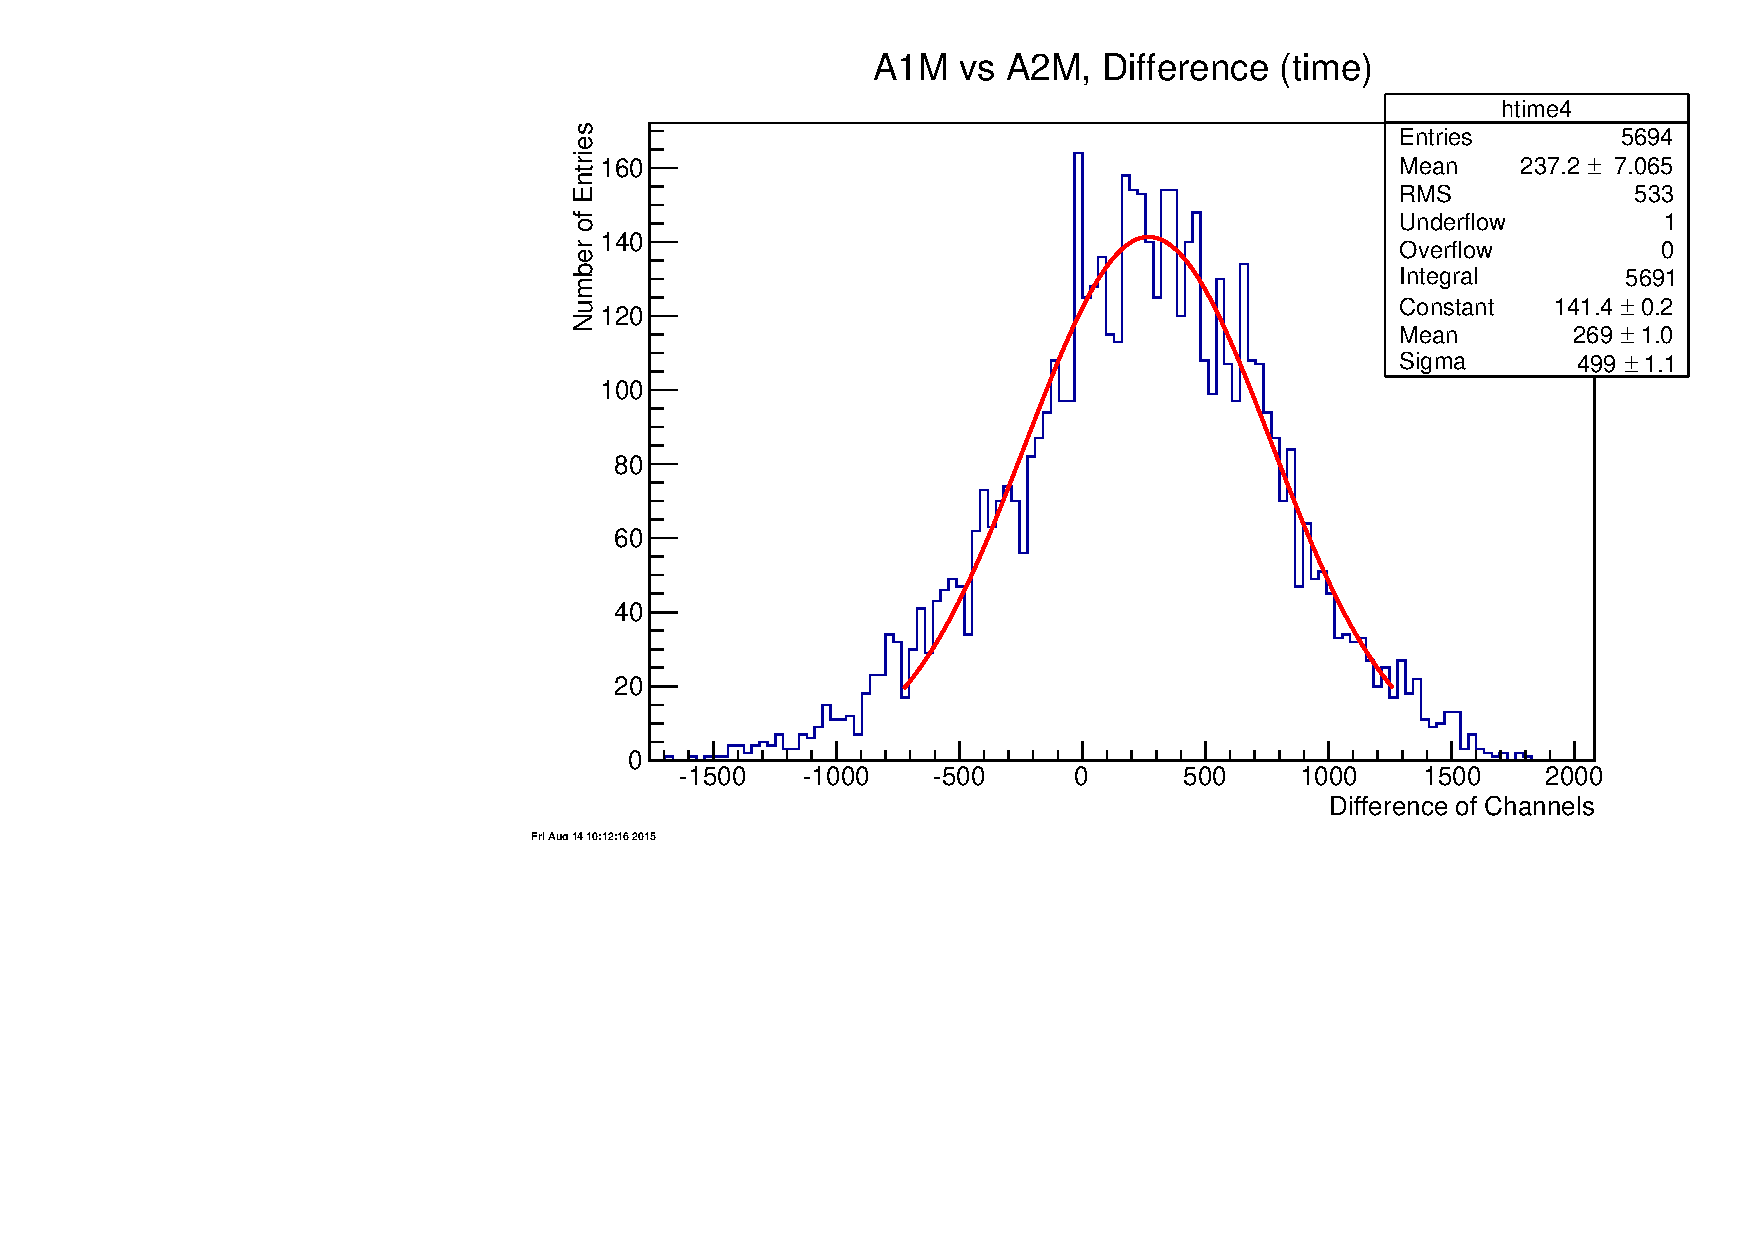
\includegraphics[width=0.4\textwidth,keepaspectratio]{run_606_htime4}\hspace{\fill}
}
\caption{(Left) Total multi-hit count spectrum from A2M. For $1\times10^6$ trigger events, 51.9\% of entries have no hits, 44.7\% of entries have exactly one hit, 3.4\% of entries have two hits, and 0.0\% of entries (3 events) have three hits. (Center) Raw data spectrum for A2M. Points corresponding to the first registered hit are shown in blue, points corresponding to the second hit are shown in red. (Right) Timing spectrum corresponding to events where both A1M and A2M have two hits; the difference of the second pair of hits is shown.
Compare with Fig.~\ref{diff_fit}.
The width of the peak 
%(499\,chan.~$\sigma$) 
is about $150\times$ that corresponding to the first pair of hits. 
}
\label{mhit}
\end{figure}

As of this writing, the multi-hit data for histogram sorting (\texttt{ana.cxx}) and tree sorting (\texttt{ana\_tree.cxx}) do not match. See Fig.~\ref{tree_comp} for details. The figure is generated with the following command.
\vsetroot
\begin{quote}
\begin{Verbatim}[firstnumber=0]
treecomp(0)
\end{Verbatim}
\end{quote}
\vsetnone
The cause of the mis-match is unknown is unknown.

\begin{figure}
\centering
\hspace{\fill}
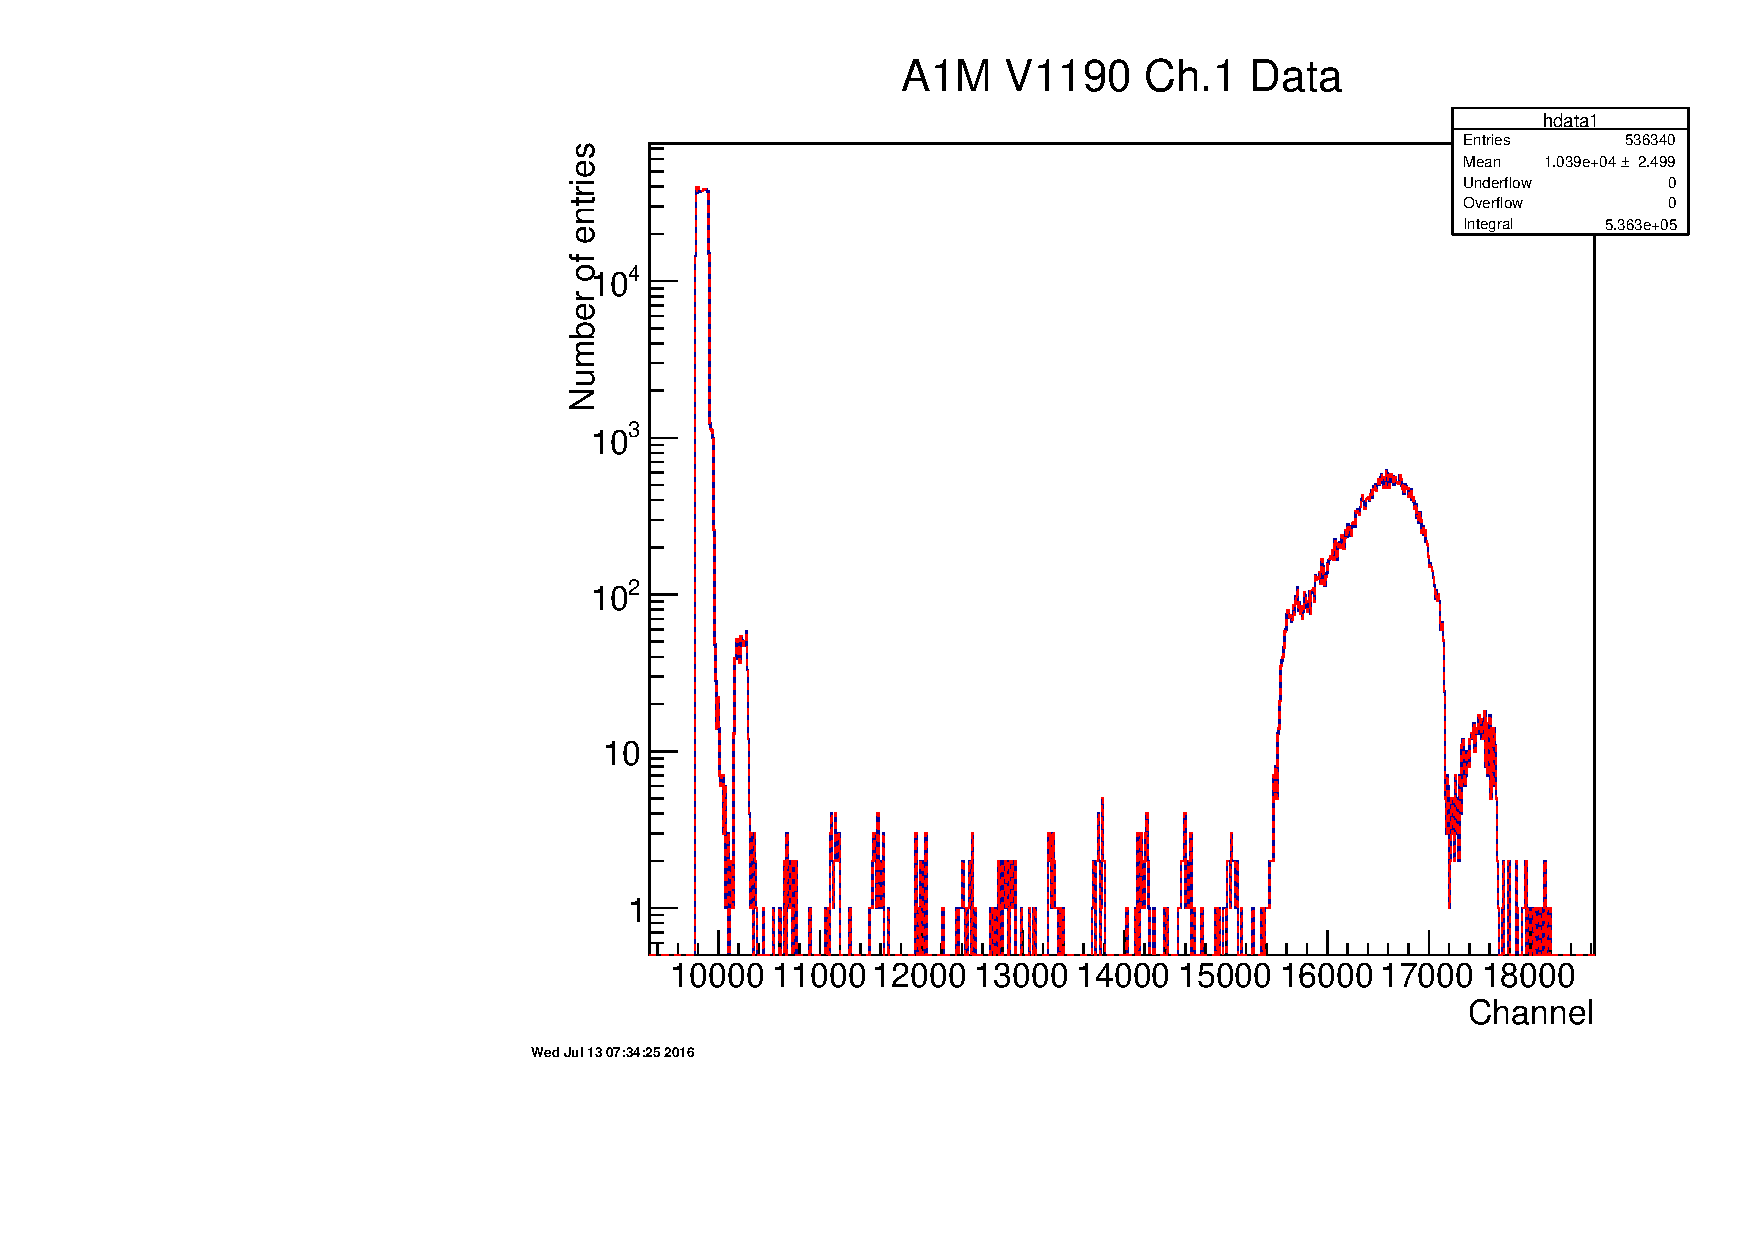
\includegraphics[width=0.48\textwidth, keepaspectratio]{run_606_treecomp1}\hspace{\fill}
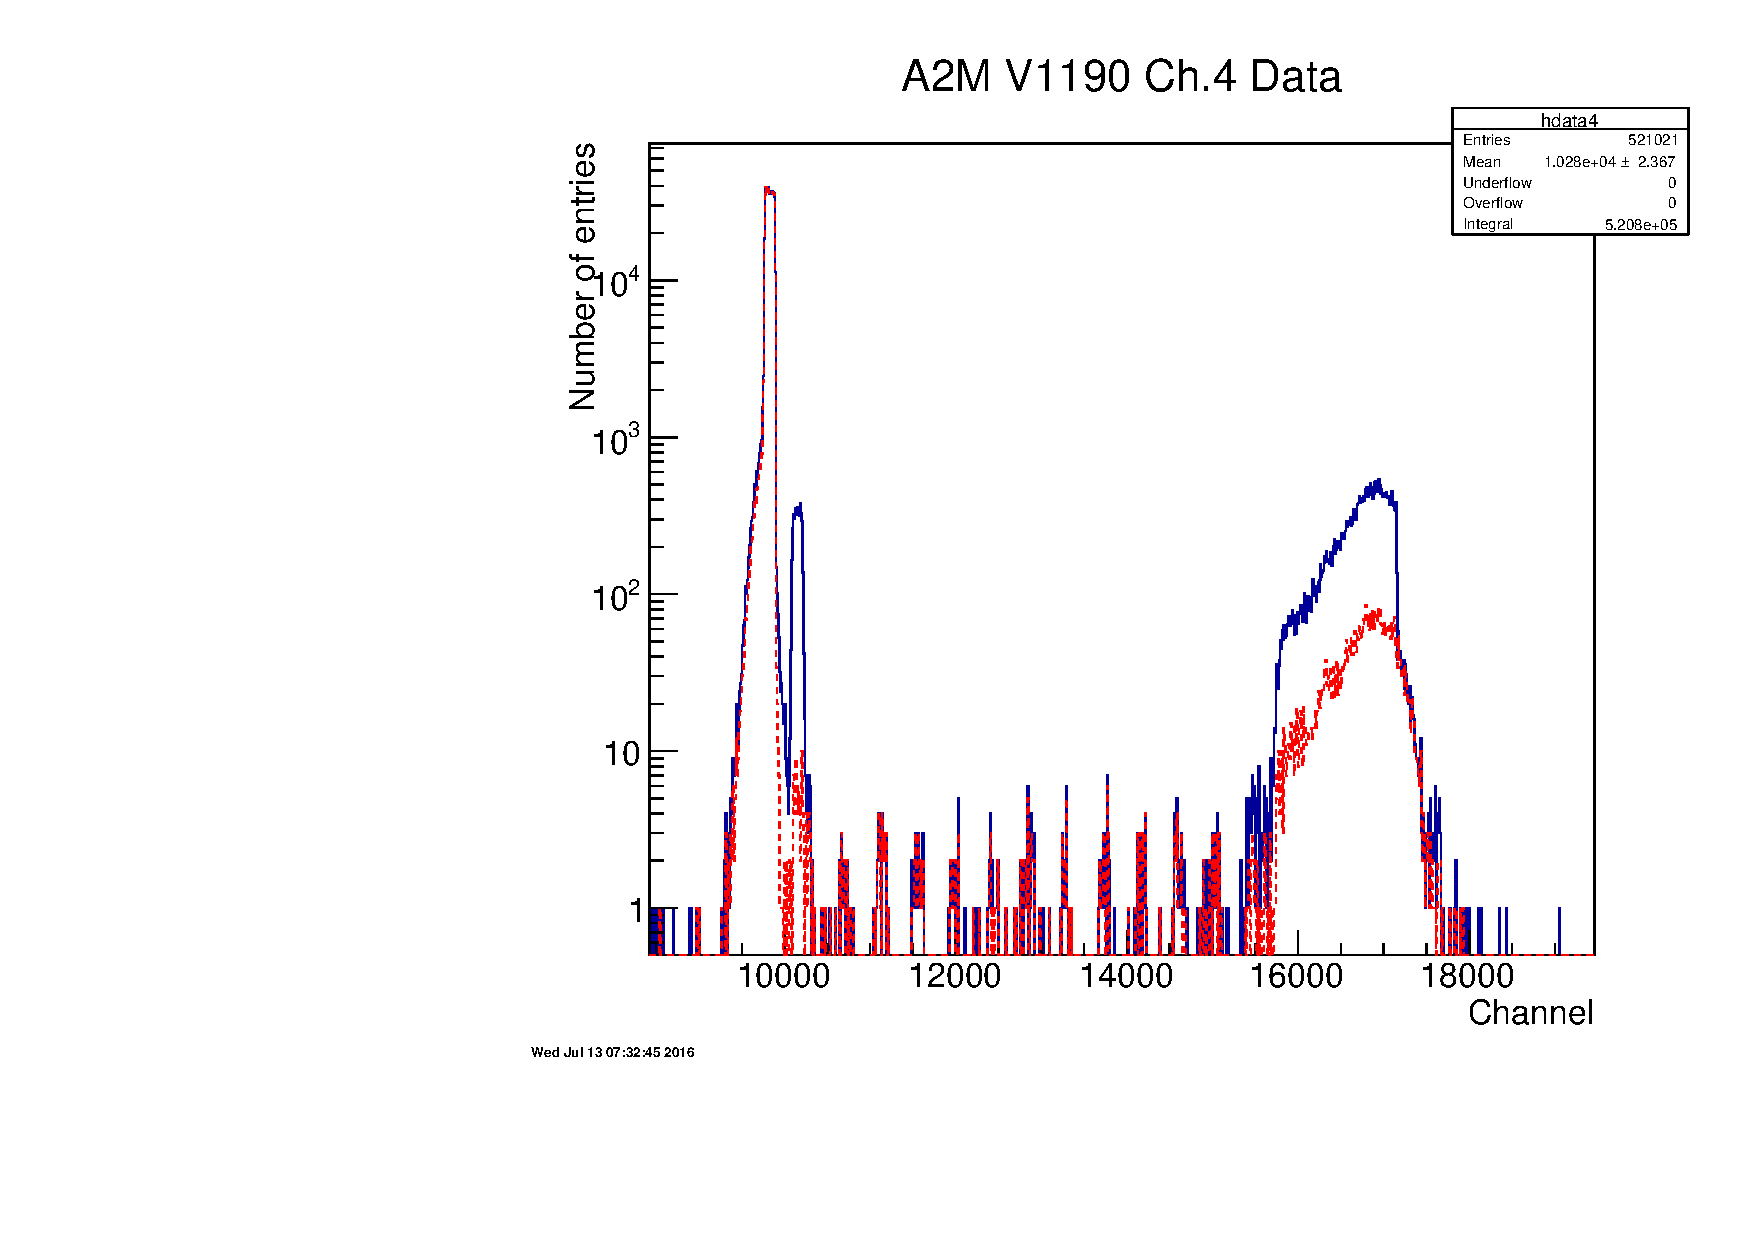
\includegraphics[width=0.48\textwidth, keepaspectratio]{run_606_treecomp4} \hspace{\fill}
\caption{Comparison of histogram sorting (blue, solid) and tree sorting (red, dashed) for anode A1M (left) and A2M (right). The two sorting methods agree for A1M, but disagree for A2M. The cause is unknown. In this example, the number of counts sorted into trees is 97\% of the counts sorted into histograms for A2M.}
\label{tree_comp}
\end{figure}


\subsection{Gain-matching}
\fussy
The first step in calibrating the detector data is to gain-matching each pair of detector signals.  Each of the 14 signals read out of the PGAC box is part of a pair.  Each cathode has a pair of signals (two pairs on each detector, four pairs in total) and each segment of the anode on each detector forms a pair (three in total).
\subsubsection{Anode Pairs}
\paragraph{Procedure}
\begin{sloppypar}
The two anodes measure the ionization from the same event in close proximity to each other ($\Delta z=36.80$\,mm).  Examining Fig.~\ref{lin_fit}\,(Left), one sees that the correlation between the anode timing signal pairs is sharply defined, linear, and the correlation coefficient is approximately equal to $+1$.  %Due to this approximate correlation,
%The timing signals from the two anodes is gain-matched such that the correlation coefficient is made 
This coefficient can be determined by plotting one of the signals in the pair against the other.  Using the \texttt{TProlile} class in ROOT, such a two-dimensional histogram may be fit with a one-dimensional function; in this case a linear polynomial.  This process is illustrated in Fig.~\ref{lin_fit}\,(Right). % for the anode signals.
This figure is generated using a command similar to the following.
\vsetroot
\begin{quote}
\begin{Verbatim}[firstnumber=0]
fitpfx("haaz4", 9700, 10100,9830,9950,1,0,0)
\end{Verbatim}
\end{quote}

\end{sloppypar}

\begin{figure}
\centering
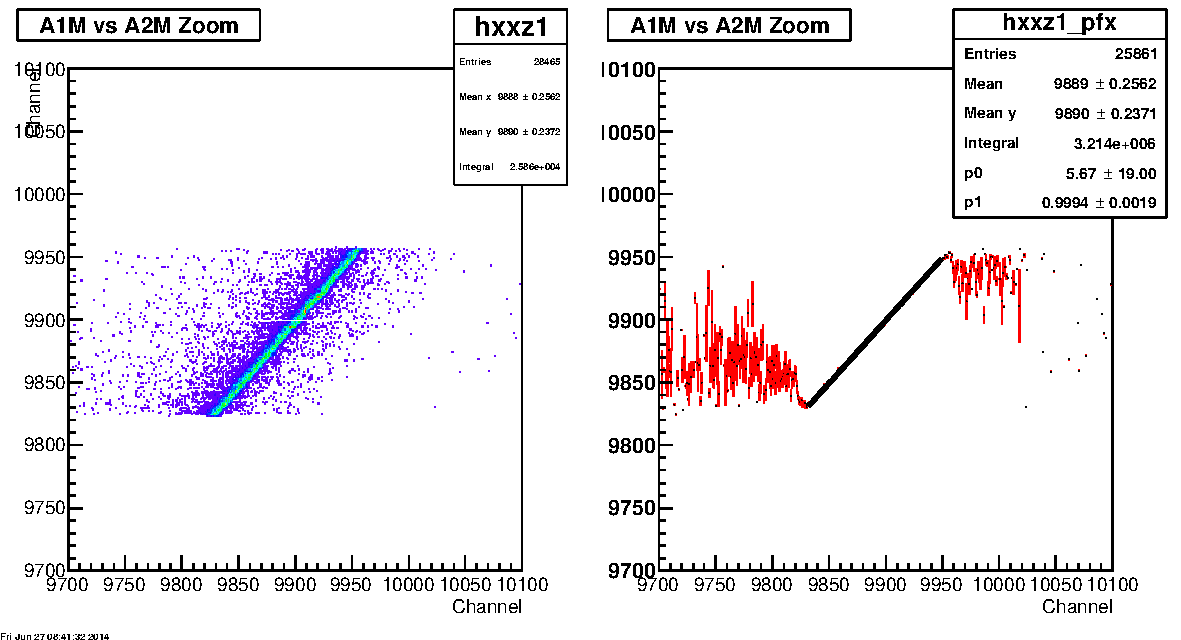
\includegraphics[width=\textwidth,keepaspectratio]{run00480_hxxz1_pfx}
\caption{Correlation plot of the anode signals.  (Left) A 2D histogram of A1M plotted against A2M is shown.  The histogram range is confined to the area of interest.  Note that the range of the signal A1M has sharp cutoffs because the anode signal from detector 1 is used to generate the trigger and is therefore self-gating. (Right) A 1D profile of the 2D histogram is fit with a linear function.}
\label{lin_fit}
\end{figure}

The quality of the linear fit verifies that the pairs of anode signals are linearly correlated.  Higher-order corrections are not necessary.  With such sharply correlated data, the slope of the fit %provides 
is closely related to the the correlation coefficient.  The goal of gain-matching the anode pairs is to minimize the width of the distribution of difference the signals.  When this is accomplished, the correlation coefficient is approximately equal to $+1$. %, thus gain-matching the signals,

\paragraph{Method}
To first order, the gain-matching is accomplished by scaling the signal plotted as the ordinate ($y$-axis) by the slope of the fit.  For the anode pairs, the signal from detector 1 is plotted on the $y$-axis.  The gain-matching technique is implemented for the anodes using the following block of code. The calibration parameters are read in from a file at the start of the analysis.  The calibration files are named for the run number, such as \texttt{run\_480.cal}.
\vspace{0.5\baselineskip}
\par\noindent
\begin{minipage}{\linewidth}
  \singlespace
\begin{lstlisting}[caption={Gain-match andode. Here the uncalibrated signal \texttt{a[i][0]} is scaled in two steps.   First, with scaling parameter derived from the slope, \texttt{hxxcal[i][1]}; and then with an offset parameter \texttt{hxxcal[i][0]}.
  The output is saved in \texttt{a[i][1]}.
The fit parameters of each correlation plot are stored in the array \texttt{hxxcal[i][j]}.  The index \texttt{[i]} runs from 0--3 for each of the 3 signal pairs and the index \texttt{[j]} runs from 0--1 for the linear fit parameters; 0 for offset, 1 for slope.}]
if(docal) { 
  a[i][1]=a[i][0]/hxxcal[i][1];	 
  a[i][1]-=hxxcal[i][0];
}
\end{lstlisting}
%a1/=hxxcal[i][1];	 
%a1-=hxxcal[i][0];
%\vspace{-1\baselineskip}
\end{minipage}


The gain-matching can be fine-tuned by adjusting the scaling parameter to minimize the  difference of the anode signal pairs.  In other words, the scale parameter is adjusted to minimize the measured width $\sigma$ of a Gaussian fit of the distribution.  This procedure is illustrated in Fig.~\ref{diff_fit}.  When the %With a
 correlation coefficient identically equal to $+1$, the difference of the anode signals should be constant; in this case equal to zero. %In a similar manner, the 
 Accordingly, the offset parameter \texttt{hxxcal[i][0]} is fine-tuned to adjust the mean of the difference to zero. Typical calibration parameters are shown in Table~\ref{anode-calib}.
 
\begin{table}[ht]
\centering  
\begin{tabular}{c..}
\hline
\multicolumn{1}{c}{Pair}& \multicolumn{1}{c}{Offset}& \multicolumn{1}{c}{Slope} \\
\multicolumn{1}{c}{\texttt{i}}&\multicolumn{1}{c}{\texttt{hxxcal[i][0]}}&\multicolumn{1}{c}{\texttt{hxxcal[i][1]}}\\ \hline \hline
 0 & 16.652191 & 0.999918377\\
 1 & 11.5593   & 0.999854499\\
 2 & 3.80868   & 0.999757652\\
 \hline 
\end{tabular}
\caption{Typical calibration constants for each of the three  anode pairs (\texttt{i}). Parameters are given for run 606. The average value of \texttt{hxxcal[i][1]} is different from 1 by an average value of 2/10,000. 
%can be correlated with each of the three anode segment pairs (\texttt{k}); twelve combinations in total. The index runs from 0--11 and is defined by $(\texttt{i}-3)\times 3 + \texttt{k}$.
}
\label{anode-calib}
\end{table}
 
\begin{figure}[ht]
\centering
\hspace{\fill}
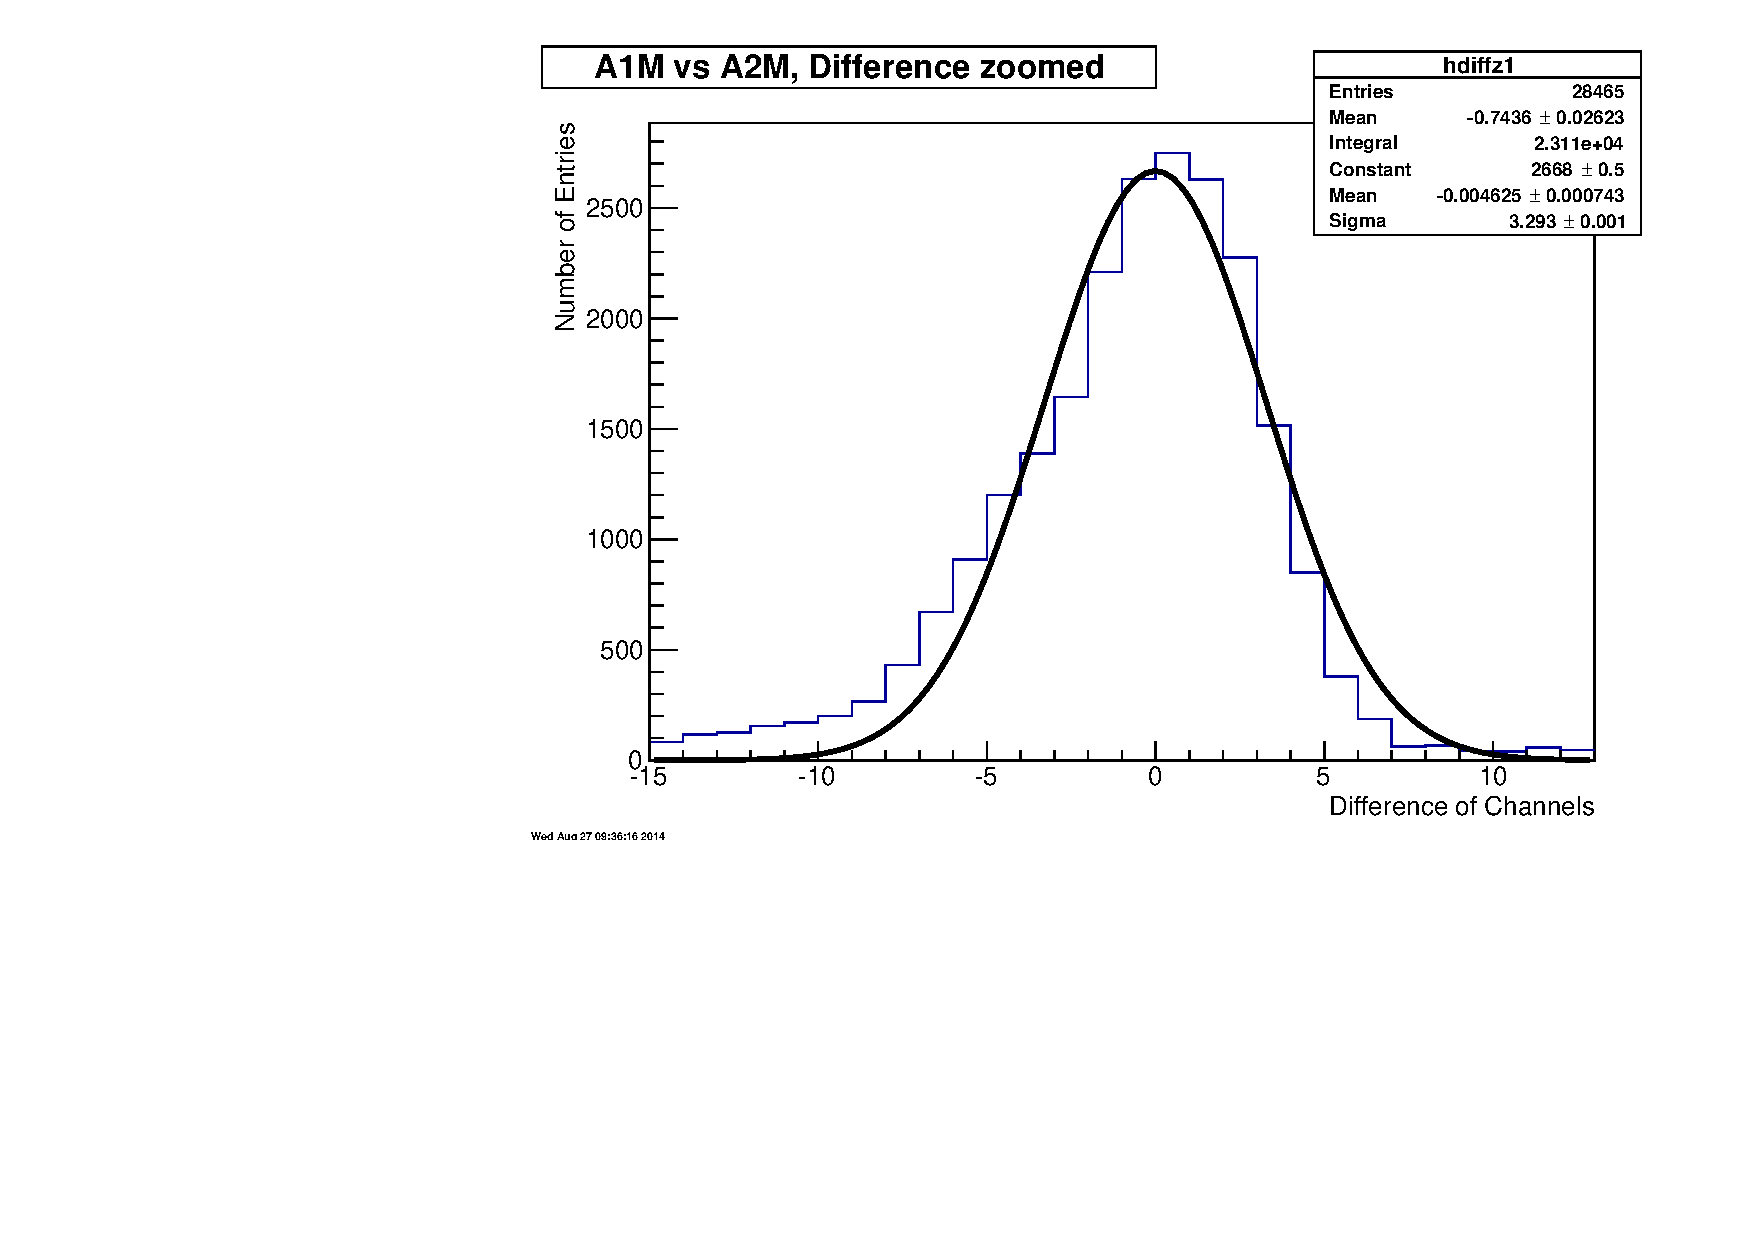
\includegraphics[width=0.48\textwidth,keepaspectratio]{run_480_hdiffz1_fit}\hspace{\fill}
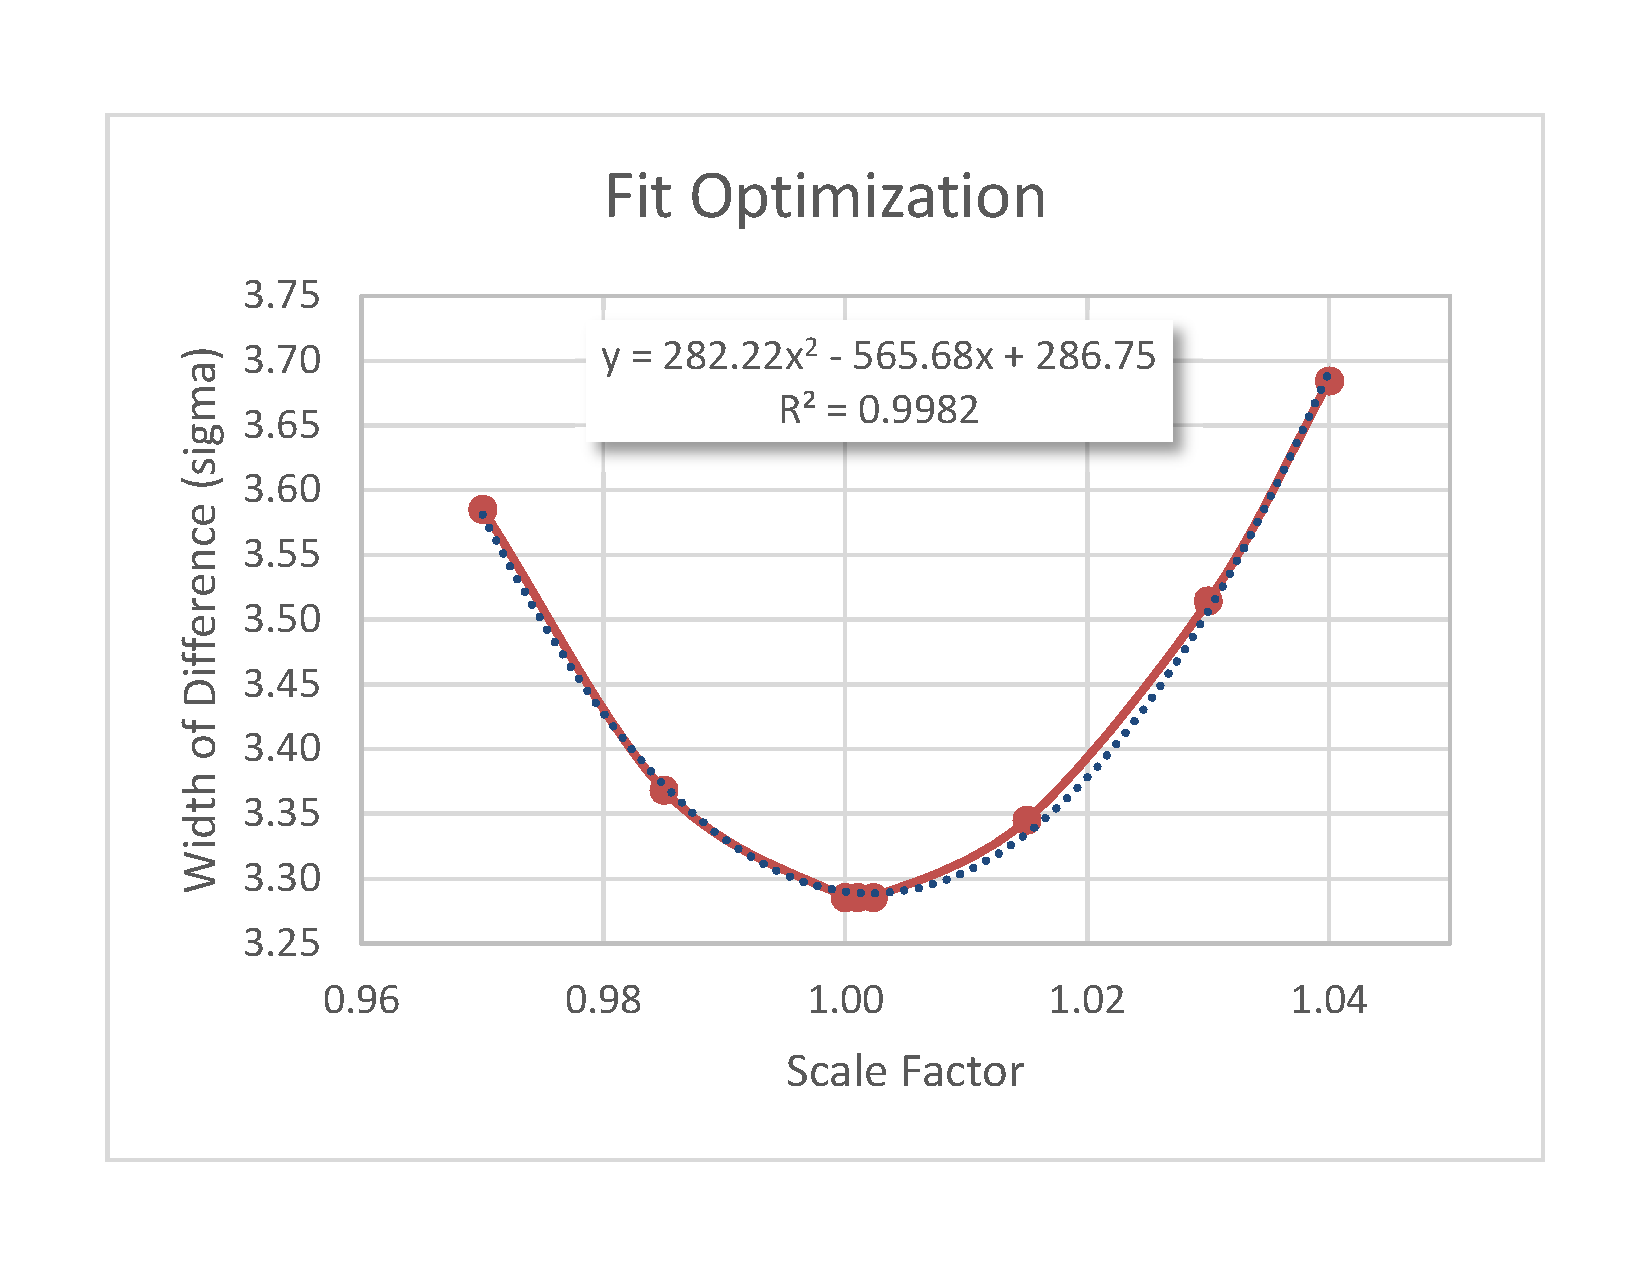
\includegraphics[width=0.48\textwidth, keepaspectratio]{hdiffz1} \hspace{\fill}
\caption{(Left) The %sum of 
difference of the anode signals are plotted and fit with a gaussian function %with X1R
after one of the positions has been scaled by %with a given 
the value of the parameter \texttt{hxxcal[1][1]}.  (Right) The value of the sigma of the gaussian fits is plotted against the scaling factor  \texttt{hxxcal[1][1]}.  The distribution is then fit with a quadratic function to calculate the best fit, in this case $1.00231$.}
\label{diff_fit}
\end{figure}

\subsubsection{Cathode Pairs}
\paragraph{Procedure}
Each pair of position signals from the cathodes are also linearly correlated.  The origin of this correlation is derived from the physical characteristics of the detector.  First, as discussed in \S\,\ref{position_description}, the delay applied to each position signal is directly-proportional to the distance of the incident ionization from each end of the detector.  Explicitly, this means that events closer to the edge of the detector have a smaller delay. Second, the sum of the delays for each position signal pair is constant (because the length of the detector is constant).  Therefore, the correlation coefficient between cathode pairs should be identically equal to $-1$. A correlation plot for a pair of position signals is shown in the appendix in Fig.~\ref{reflect}\,(Left). As is the case with the anode signals, the cathode signals can be gain-matched by scaling one of the signals by a linear offset.
\paragraph{Method}
The gain-matching technique is implemented for the cathodes using the following block of code.
%\pangram{100}
\vspace{0.5\baselineskip}
\par\noindent
\begin{minipage}{\linewidth}
  \singlespace
\begin{lstlisting}[caption={The index \texttt{i} runs over 3--6 for each cathode pair. Here \texttt{xn[i-3][0]} refers to the (uncalibrated) ``near'' position signal and \texttt{xf[i-3][0]} refers to the ``far'' position signal.  These labels correspond to those given in Table~\ref{TDC_signals} and are defined from the perspective of the beam.   The nested \texttt{if} statement is used so that neither signal is compressed; one of the signals is expanded to set the correlation coefficient to $-1$.},label=cathode_scaling]
if(docal) {
  if(hxxcal[i][1]<-1.) {
    xn[i-3][1]=xn[i-3][0]*(-hxxcal[i][1]);
    xf[i-3][1]=xf[i-3][0];
  }
  else {
    xn[i-3][1]=xn[i-3][0]; 
    xf[i-3][1]=xf[i-3][0]*(-1./hxxcal[i][1]);
  }
}
\end{lstlisting}
%   xn=(-hxxcal[i][1])*xn;
%  }
%  else{
%    xf=(-1./hxxcal[i][1])*xf;
%  }
%}
%\vspace{-1\baselineskip}
\end{minipage}

%\subsubsection{Verification}
As previously stated, the sum of the position signals should be constant.
% and the difference of the anode signals should be constant.
In a manner similar to that used with the anode signals, %Therefore, 
the scale factor can be adjusted to minimize the width of the sum of the position signals. % and the difference of the anode signals. 
 This procedure is illustrated in Fig.~\ref{sum_fit}. 
\begin{figure}
\centering
\hspace{\fill}
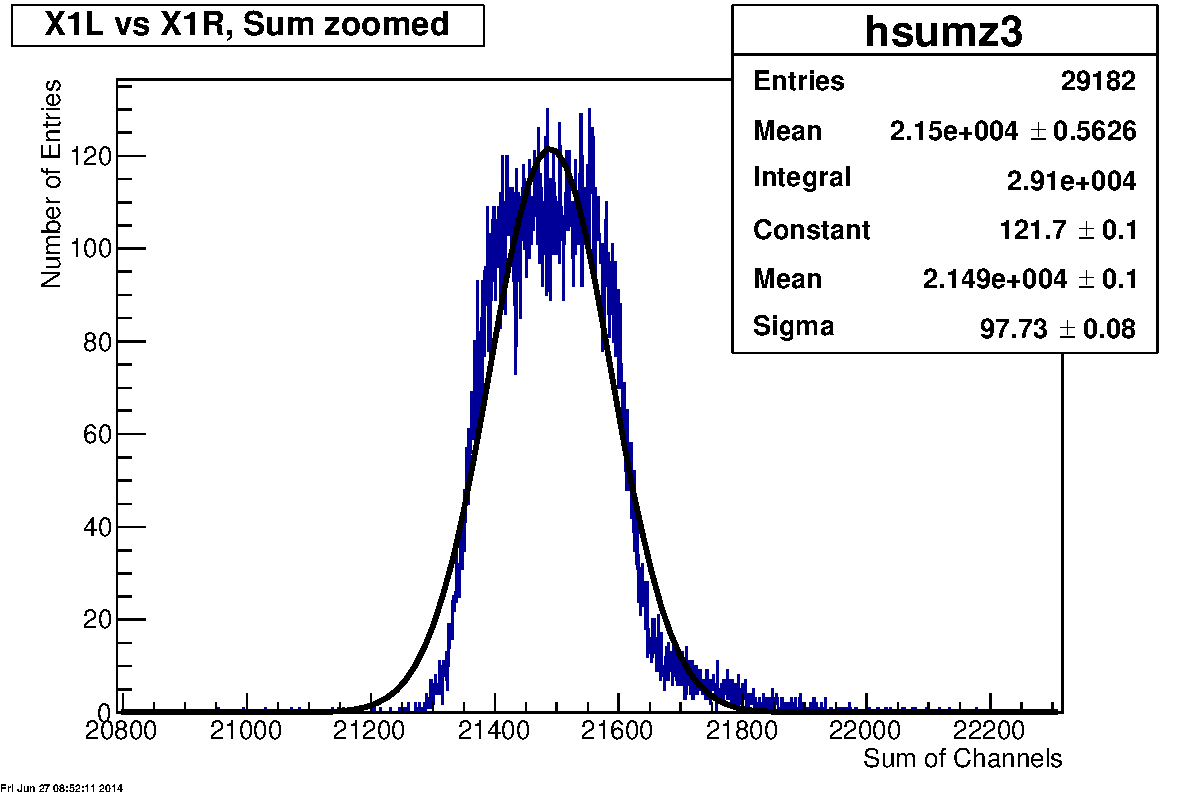
\includegraphics[width=0.48\textwidth,keepaspectratio]{run00480_hsumz3}\hspace{\fill}
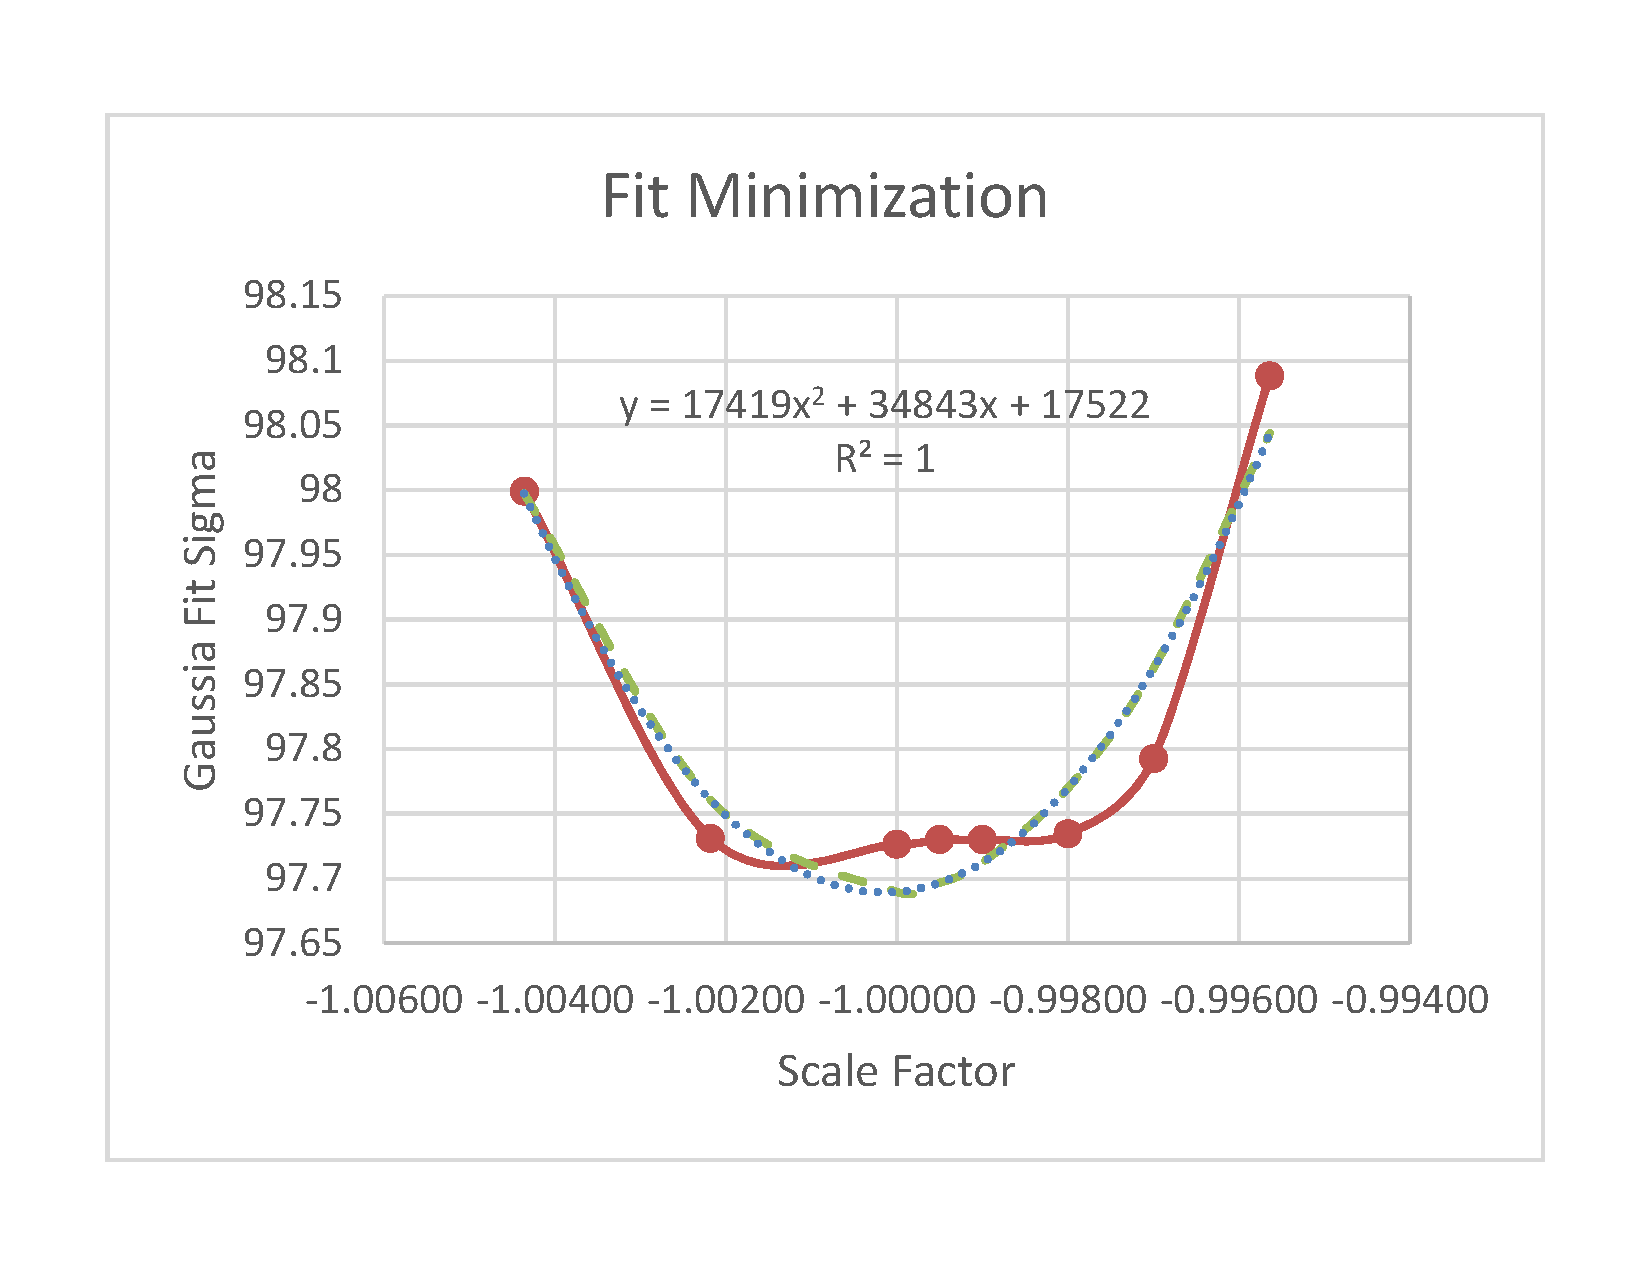
\includegraphics[width=0.48\textwidth, keepaspectratio]{hsumz3_fit} \hspace{\fill}
\caption{(Left) The %sum of 
position signals X1L and X1R are summed and fit with a gaussian function %with X1R
after one of the positions has been scaled by %with a given 
the value of the parameter \texttt{hxxcal[3][1]}.  (Right) The value of the sigma of the gaussian fits is plotted against the scaling factor  \texttt{hxxcal[3][1]}.  The distribution is then fit with a quadratic function to calculate the best fit, in this case $-1.00015$.}
\label{sum_fit}
\end{figure}
In this example, the width of the sum of the position signals X1L and X1R was measured for several values of the scaling parameter \texttt{hxxcal[3][1]}.  The resulting distribution was fit with a quadratic function to locate the value of \texttt{hxxcal[3][1]} that corresponds to the minimum width of the sum. Table~\ref{cathode-calib} shows some typical calibration values.

\begin{table}[ht!]
\centering  
\begin{tabular}{c..}
\hline
\multicolumn{1}{c}{Pair}& \multicolumn{1}{c}{Offset}& \multicolumn{1}{c}{Slope} \\
\multicolumn{1}{c}{\texttt{i}}&\multicolumn{1}{c}{\texttt{hxxcal[i][0]}}&\multicolumn{1}{c}{\texttt{hxxcal[i][1]}}\\ \hline \hline
 3 & 0 & -1.00152409\\
 4 & 0 & -1.002232225\\
 5 & 0 & -1.000613607\\
 6 & 0 & -0.995592661\\
 \hline 
\end{tabular}
\caption{Typical calibration constants for each of the 4 cathode pairs (\texttt{i}). Given for run 480. The average value of \texttt{hxxcal[i][1]} is different from -1 by an average value of 2/1,000. 
Note that the offset variable is not used.
%can be correlated with each of the three anode segment pairs (\texttt{k}); twelve combinations in total. The index runs from 0--11 and is defined by $(\texttt{i}-3)\times 3 + \texttt{k}$.
}
\label{cathode-calib}
\end{table}

%\subsubsection{Anode Segments}
\subsubsection{Anode-Cathode}
\paragraph{Procedure}
Comparing the gain-matching procedure for the anodes and cathodes, two particular features are evident. First, the width of the correlations  for the cathodes appears to be much broader than that of the anodes (compare Fig.~\ref{lin_fit}\,(Left) with Fig.~\ref{reflect}\,(Left) in the Appendix).  Second, the width of the difference of the anode signals is more sharply defined and responds to scaling in a more predicable manner than the sum of the cathode signals (compare Fig.~\ref{diff_fit} with Fig.~\ref{sum_fit}).  The origin of this discrepancy can be revealed by comparing the cathode pairs with their corresponding anode. 

Each cathode pair can be correlated to an anode signal.  There are four cathode pairs in total corresponding to the two position pairs are each of the two detectors. There are three anodes %pairs
 corresponding to the three %anode 
 segments on each detector. This configuration yields twelve possible combinations.  The combinations are summarized in Table.~\ref{position-andode}.  For example, the sum of the Y2 signals are plotted against the anode signal of detector 2 in Fig.~\ref{hsa}.  By inspection, it can be seen that the sum of the position signals varies with the anode signal.  However, as discussed, the sum of the cathode signals should be constant.
\begin{table}[ht!]%
\centering  
\begin{tabular}{ccccc}
%\begin{tabulary}{1.0\textwidth}{ccccc} 
\hline
\multicolumn{1}{c}{Index} & \multicolumn{1}{c}{Pair}& \multicolumn{1}{c}{Segment}& Position & Anode \\
&\multicolumn{1}{c}{\texttt{i}}&\multicolumn{1}{c}{\texttt{k}}\\ \hline \hline
 0 & 3 & 0 & \texttt{X1} & \texttt{A1B} \\
 1 & 3 & 1 & \texttt{X1} & \texttt{A1M} \\
 2 & 3 & 2 & \texttt{X1} & \texttt{A1T} \\
 3 & 4 & 0 & \texttt{Y1} & \texttt{A1B} \\
 4 & 4 & 1 & \texttt{Y1} & \texttt{A1M} \\
 5 & 4 & 2 & \texttt{Y1} & \texttt{A1T} \\
 6 & 5 & 0 & \texttt{X2} & \texttt{A2B} \\
 7 & 5 & 1 & \texttt{X2} & \texttt{A2M} \\
 8 & 5 & 2 & \texttt{X2} & \texttt{A2T} \\
 9 & 6 & 0 & \texttt{Y2} & \texttt{A2B} \\
10 & 6 & 1 & \texttt{Y2} & \texttt{A2M} \\
11 & 6 & 2 & \texttt{Y2} & \texttt{A2T} \\
 \hline 
\end{tabular}
%\end{tabulary}
\caption{Each of the four position pairs (\texttt{i}) can be correlated with each of the three anode segment pairs (\texttt{k}); twelve combinations in total. The index runs from 0--11 and is defined by $(\texttt{i}-3)\times 3 + \texttt{k}$.}
\label{position-andode}
\end{table}
\begin{figure}[ht]
\centering
\hspace{\fill}
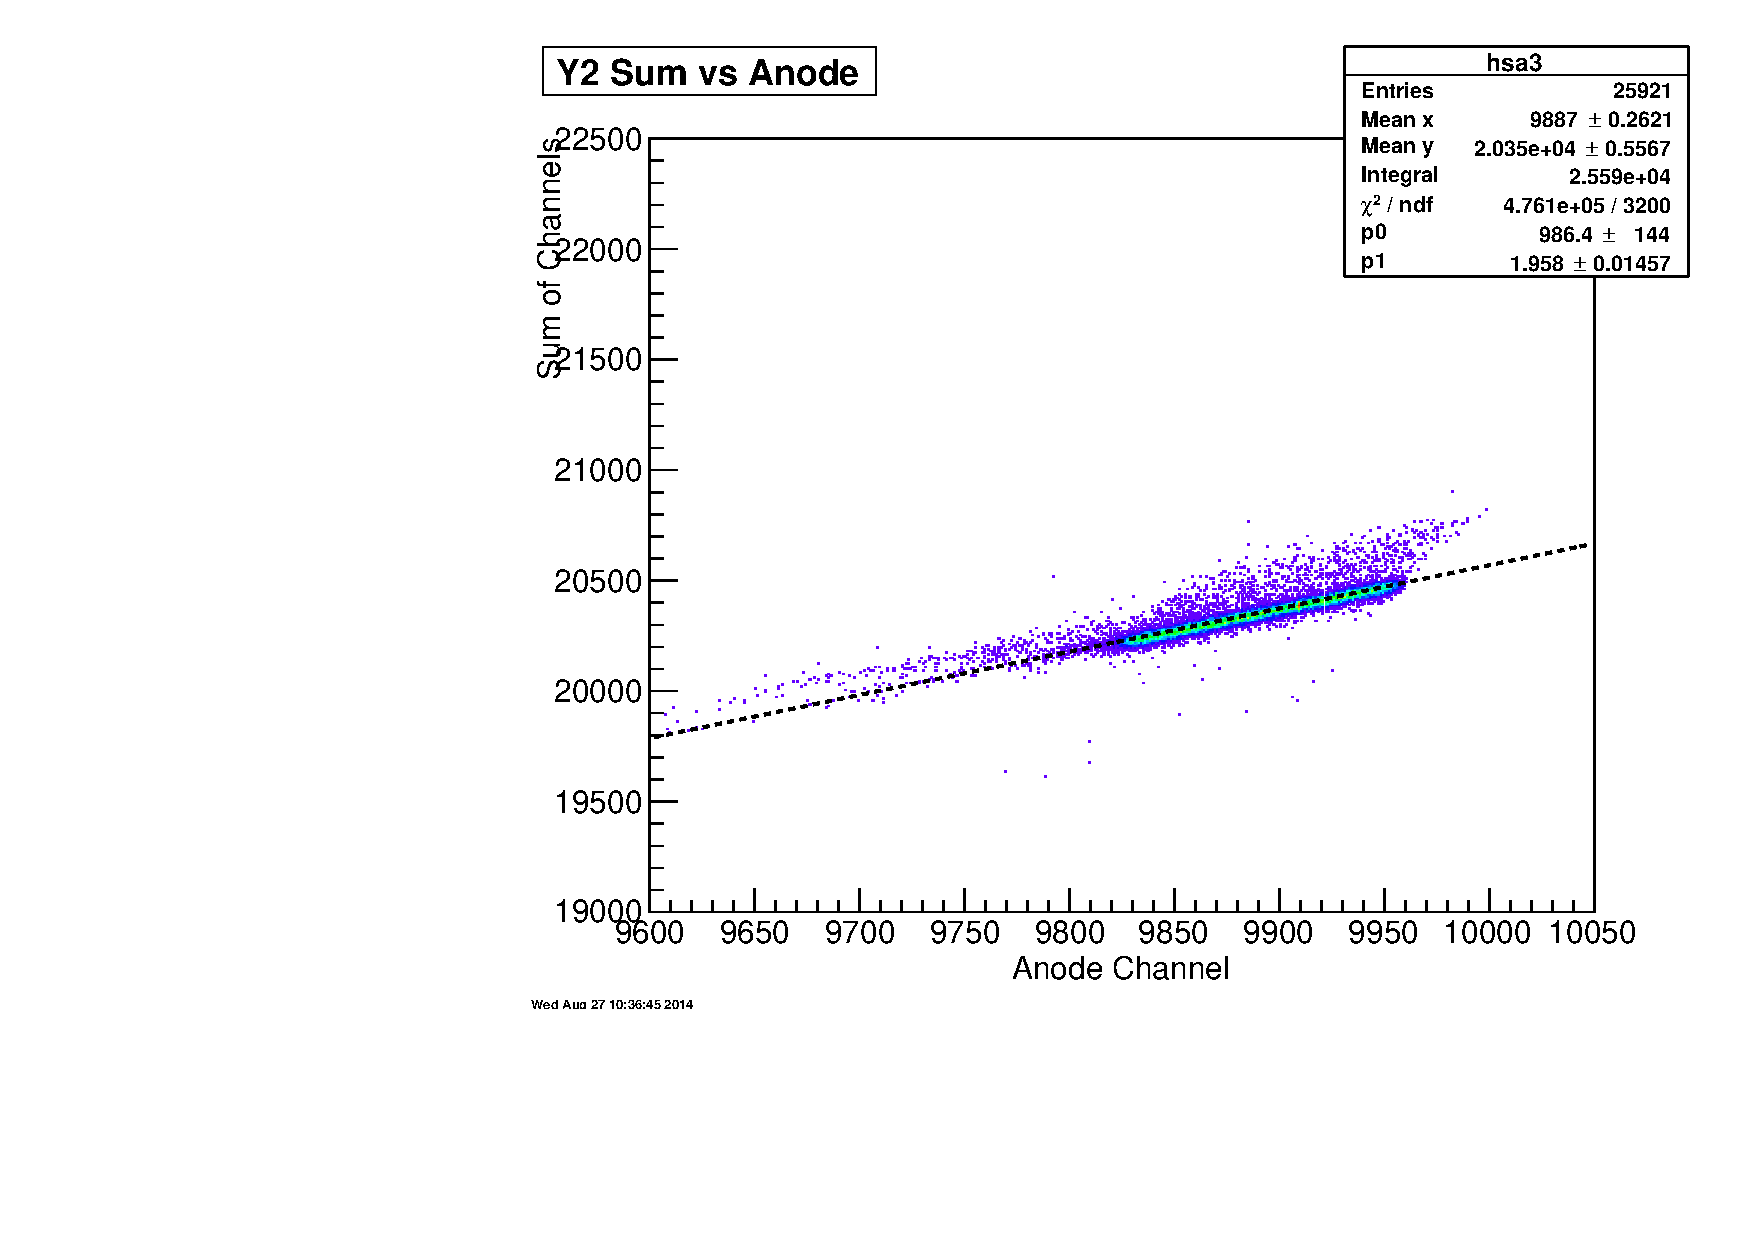
\includegraphics[width=0.48\textwidth, keepaspectratio]{run_480_hsa3_fit}\hspace{\fill}
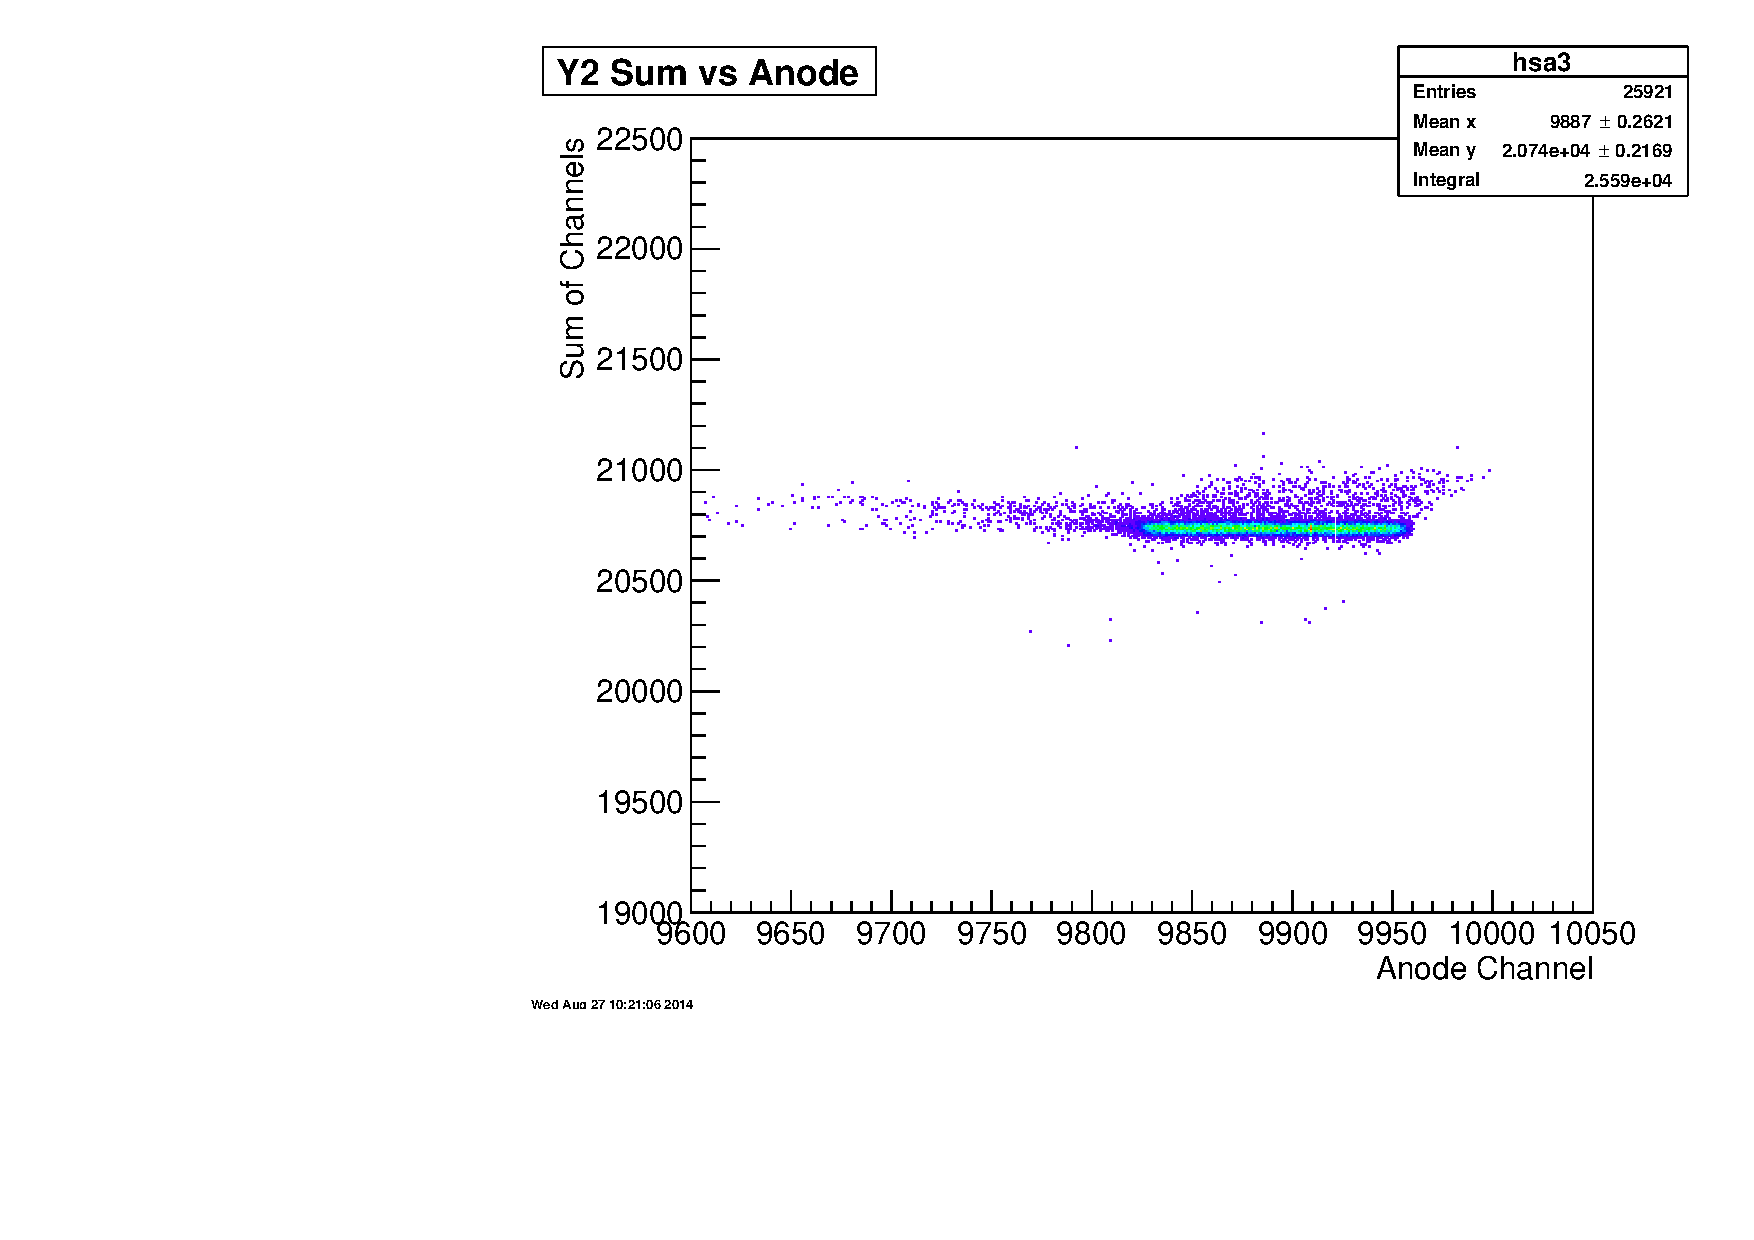
\includegraphics[width=0.48\textwidth, keepaspectratio]{run_480_hsa3_cor} \hspace{\fill}
\caption{The sum of the Y2 position signals are plotted against the sum of the anode signals.
(Left) The uncorrected correlation is plotted with a linear fit overlaid on the data.
(Right) The correlation is plotted after correcting for the slope.  The sum of the cathode signals is now constant.}
\label{hsa}
\end{figure}

\paragraph{Method}
The linear variation of the sum of the cathode signals as a function of the anode signal can be corrected with the following block of code.
\vspace{0.5\baselineskip}
\par\noindent
\begin{minipage}{\linewidth}
  \singlespace
\begin{lstlisting}[caption={Here the index \texttt{i} runs over 3--6, corresponding to the cathode signal pairs and \texttt{k} runs over 0--2, corresponding to the anode signal; as defined in Tables~\ref{TDC_signals} and \ref{position-andode}. The expression \texttt{(int)((i-3)/2)} has a value of 0 or 1 and selects the detector number. The expression \texttt{k+3*(int)((i-3)/2)} has a value of 0--5 
%1 or 4 
and selects the anode signal. See the text for further details.
},label=anode-cathode-eq]
if(a[k+3*(int)((i-3)/2)][1]>0) {
  xn[i-3][2]=xn[i-3][1]-(a[k+3*(int)((i-3)/2)][1]
                         *hasumcal[((i-3)*3)+k][1])/2;
  xn[i-3][2]+=hasumcal[((i-3)*3)+k][2]/2;
  xf[i-3][2]=xf[i-3][1]-(a[k+3*(int)((i-3)/2)][1]
                         *hasumcal[((i-3)*3)+k][1])/2;
  xf[i-3][2]+=hasumcal[((i-3)*3)+k][2]/2;
}
\end{lstlisting}
%xn-=(A[1+3*(int)((i-3)/2)]*hasumcal[i-3][1])/2-hasumcal[i-3][2]/2;
%xf-=(A[1+3*(int)((i-3)/2)]*hasumcal[i-3][1])/2-hasumcal[i-3][2]/2;
%\vspace{-1.3\baselineskip}
\end{minipage}
%\sloppy
\begin{sloppypar}

%If all three anode segments were connected independently, the ``1'' in the previous expression would be replaced with \texttt{k} and would run over 0--2.
The parameter array \texttt{hasumcal[((i-3)*3)+k][j]} holds three parameters for each possible combination of position and anode: the offset [0] and slope [1] of the linear fit, such as that  shown in Fig.~\ref{hsa}; and a second offset parameter [2].  The first two parameters are used to adjust the slope of the correlation to zero.  The second offset parameter is used to set the overall offset of the new, flattened distribution.  The sum of the position signals is arbitrarily shifted to 20,750, roughly corresponding to the average value of the uncalibrated sums of the cathode signals.  

\end{sloppypar}
\begin{table}
\centering  
\begin{tabular}{c...}
\hline
\multicolumn{1}{c}{Pair}& \multicolumn{1}{c}{Offset}& \multicolumn{1}{c}{Slope} & \multicolumn{1}{c}{Re-center} \\
\multicolumn{1}{c}{\texttt{i}}&\multicolumn{1}{c}{\texttt{hasumcal[i][0]}}&\multicolumn{1}{c}{\texttt{hasumcal[i][1]}}  &\multicolumn{1}{c}{\texttt{hasumcal[i][2]}}\\ \hline \hline
 0 & 1821.13 & 1.99218 & 18925.0 \\
 1 & 1824.38 & 1.99607 & 18925.8 \\
 2 & 1794.25 & 1.99819 & 18954.6 \\
 3 & 773.202 & 1.99094 & 19976.1 \\
 4 & 713.333 & 1.99371 & 20119.4 \\
 5 & 680.299 & 1.99967 & 20071.1 \\
 6 & 1539.11 & 2.01388 & 19171.5 \\
 7 & 1610.62 & 2.01017 & 19137.6 \\
 8 & 1474.61 & 2.01852 & 19202.7 \\
 9 & 660.381 & 2.00130 & 20095.6 \\
10 & 366.884 & 2.00641 & 20136.4 \\
11 & 1806.45 & 1.99139 & 20039.9 \\
 \hline 
\end{tabular}
\caption{Typical calibration constants for each of the twelve possible anode-cathode pairs (\texttt{i}).
The indices are the same as those shown in Table~\ref{position-andode}.
 Parameters are given for run 606. The slope parameter \texttt{hasumcal[i][1]} corrects the slope of the given cathode sum as a function of the given anode signal. 
%can be correlated with each of the three anode segment pairs (\texttt{k}); twelve combinations in total. The index runs from 0--11 and is defined by $(\texttt{i}-3)\times 3 + \texttt{k}$.
}
\label{anode-cathode-calib}
\end{table}


The results of this procedure are shown in Fig.~\ref{pos_cor}. This figure is generated with a command similar to the following (updated to reflect development of the analysis code).
\vsetroot
\begin{quote}
\begin{Verbatim}[firstnumber=0]
getressum("hsumz3","hxfxnznn3")
\end{Verbatim}
\end{quote}
\vsetnone
 By adding the same adjustment to each of the position signals, the difference of the position signals is unaffected.  The equations given in the next section show that by changing the value of the sum of the position signals, the calculated position will be altered.  However, using this method the sum of the position signals is made constant (as it should be). Furthermore, a linear position calibration will correct (undo) any change in the position caused by this refinement. The calibration constants obtained by the methods described in this section are stable and constant (on the order of 0.1\%) across all runs; this includes all detector settings and beam currents. The default calibration constants for the 2014 test are derived from run ; and the default for the 2015 tests are from run 606.

Inspection of Code Block~\ref{anode-cathode-eq} reveals that iterative application of this technique is additive. That is, if after applying the calibration constants, a test-fit reveals that the anode-dependence of the cathode sum is not completely removed, the new calibration constants are the sum of the old calibration constants. For example, if the initial fit has a slope of 2.0, and the subsequent test-fit has a slope of 0.01, the new calibration constant should be the sum of the two: 2.01. In all cases, the test fit should have a slope $\leq0.004$. Correspondingly, the sensitivity of the slope correction is about %$\frac{1}{500}$ 
1/500.
\begin{figure}
\centering
%\hspace{\fill}
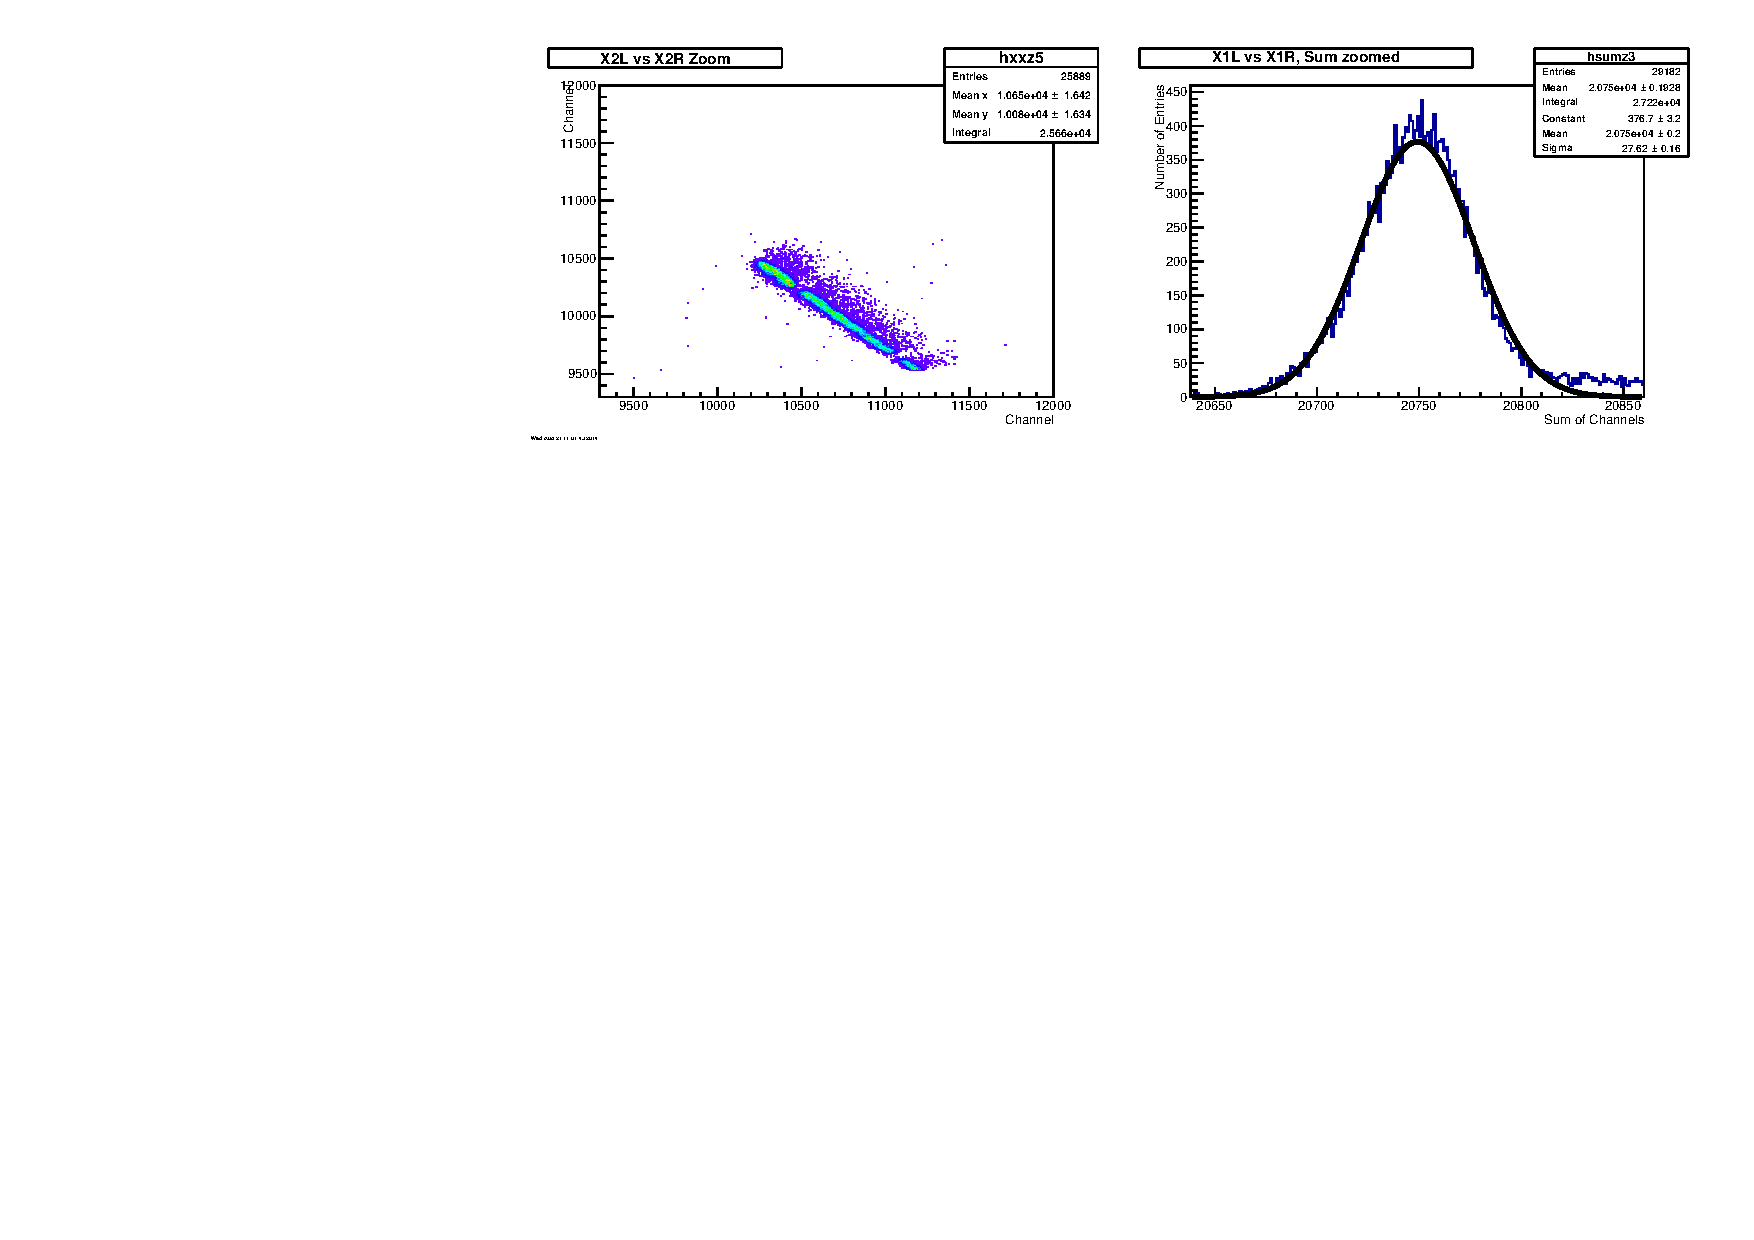
\includegraphics[width=\textwidth, keepaspectratio]{run_480_hxxz3}\hspace{\fill}
%\includegraphics[width=0.48\textwidth, keepaspectratio]{run_480_hsumz3_cor} \hspace{\fill}
\caption{(Left) Correlation plot the X2L and X2R position signals after correcting for the variations of the sum of the position signals as a function of the anode signal (cf. Fig.~\ref{reflect}). %\,(Left)).
  (Right) The sum of X2L and X2R (cf. Fig.~\ref{sum_fit}). %\,(Left)).
  Correcting for the anode variations reduces the width of the sum of the cathode signals by an average factor of $4.7\times$.}
\label{pos_cor}
\end{figure}

\subsection{Position}
\subsubsection{Definition}
The position signals may be  identified as $X_\mathrm{far}$ and $X_\mathrm{near}$, with ``far'' and ``near'' relative to one end of the detector.  To be consistent with Fig.~\ref{mask}, let us define ``near'' as the left-hand side of the detector in the $x$-direction and the bottom of the detector in the $y$-direction; both as viewed by the beam.  Recall, that the left side of the detector as viewed by the beam corresponds to the signals labeled X$n$R.
With the position derived from a delay line, the value of the delay is directly-proportional to the distance at which the ionization is detected.  As previously discussed, the sum of the position signals is effectively a measurement of the length of the delay line and is therefore constant.  %As a result, 
Combining these ideas, the position on the detector is proportional to $X_\mathrm{near}$.\footnote{Note that this is the opposite of the situation with a position-sensitive detector based on resistive division; i.e., with a position derived from resistive division, the position is proportional to the ``far'' signal divided by the sum.}
\begin{equation}
X\propto\left[\frac{X_\mathrm{near}}{(X_\mathrm{far}+X_\mathrm{near})}\right]
\label{detector_prop}
\end{equation}
The position on the detector may also be expressed in terms of the difference between he paired position signals.  When this difference is divided by the sum of the paired position signals, the result will vary over the interval $[-1,1]$.  The fractional position---that is, the position  over the interval $[0,1]$---can then be expressed as
%Express as a difference, the position on the detector may be rewritten as
\begin{equation}
\begin{split}
%X=&\frac{L}{2}\left[1+\frac{(X_\mathrm{far}-X_\mathrm{near})}{E}\right]
X=&\frac{L}{2}\left[1+\frac{(X_\mathrm{near}-X_\mathrm{far})}{(X_\mathrm{far}+X_\mathrm{near})}\right]
\label{detector_X}
\end{split}
\end{equation}
with $X=0$ corresponding to an event at the $X_\mathrm{near}$ end of the detector and $X=L$ corresponding to an event at the $X_\mathrm{far}$ end, where L is the length of the detector.  This is implemented in the code as follows.
%\pangram{10}
\vspace{0.5\baselineskip}
\par\noindent
\begin{minipage}{\linewidth}
\singlespace
\begin{lstlisting}[caption={Position definition with simple variables. The variable \texttt{xn} refers to the near side of the detector and \texttt{xf} refers to the far side of the detector.}]
x=(1/2.)*(1+((xn-xf)/(xf+xn)));//Position w/ xn@x=0 and xf@x=1 (delay).
\end{lstlisting}
\end{minipage}
%\pangram{10}
\vspace{0.5\baselineskip}
\par\noindent
\begin{minipage}{\linewidth}
\singlespace
\begin{lstlisting}[caption={Position definition with arrayed variables. Here the index \texttt{i} runs from 3--6 to cover the four pairs of positions. Each variable is a $4\times3$ array. The first index \texttt{i-3} corresponds to each position. The second index \texttt{k} corresponds to the calibration level: 0 for uncalibrated, 1 for partially calibrated, and 2 for fully calibrated.}]
for(Int_t k=0;k<3;k++) {
  x_sum [i-3][k]=xf[i-3][k]+xn[i-3][k];
  x_diff[i-3][k]=xn[i-3][k]-xf[i-3][k];
}
x[i-3][0]=(1/2.)*(1+((x_diff[i-3][2])/(x_sum[i-3][2])));
\end{lstlisting}
\end{minipage}

Again recalling that the sum of the positions signals is constant, we see from Eq.~\ref{detector_X} that the position 
%is also proportional 
has a linear relationship to the difference in the position signals.  This can be seen in Fig.~\ref{hdiffz} which plots the quantity $\textrm{X2R}-\textrm{X2L}$.  Referring to Table~\ref{TDC_signals}, we see that this difference corresponds to $(X_\mathrm{near}-X_\mathrm{far})$.  Also, when $X_\mathrm{far}$ is plotted against $X_\mathrm{near}$---as it is in Fig.~\ref{reflect}---we see that the position can also be obtained by projecting the distribution onto the line $y=-x$.
\begin{figure}
\centering
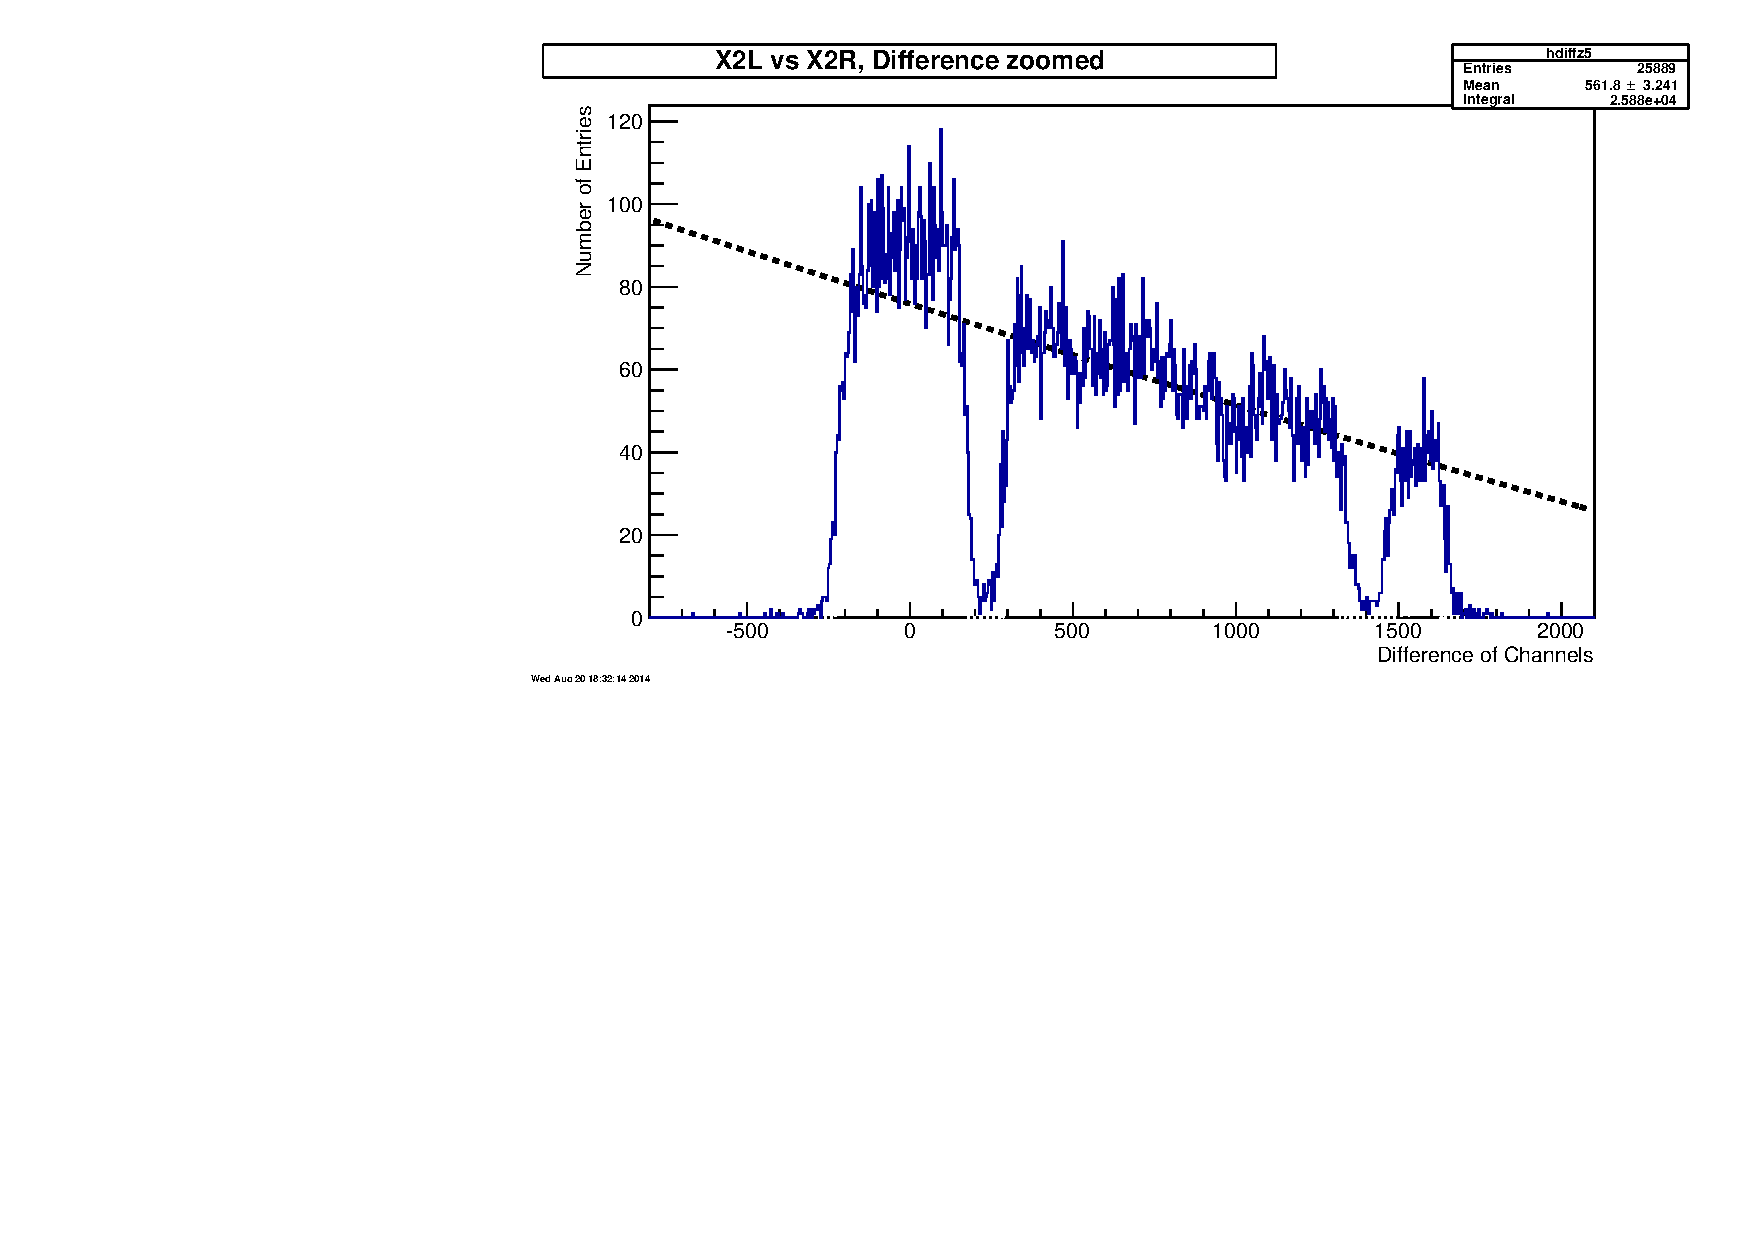
\includegraphics[width=\textwidth, keepaspectratio]{run_480_X2L_vs_X2Rg}
\caption{Example plot of the difference of paired position signals.  The gaps in the spectrum correspond to the mask shown in Fig.~\ref{mask}.  The overall distribution has been fit with a
 %$1/
$\csc^4 (\theta/2)$ function, characteristic of the Rutherford scattering cross section.
% (albeit flipped over the $y$-axix).
 The difference in channels has a linear relationship with the position.}%
\label{hdiffz}%
\end{figure}

\subsubsection{Reference Positions}
\label{cal_def}
The position calibration is based on the shadow cast by the masks shown in Figs.~\ref{mask} and \ref{mask2} onto the detector planes.  The $z$-positions of the detector planes is given in Table~\ref{zpos}.  The $z$-axis is defined by the central central beam trajectory, in this case corresponding to a polar angle of $\theta=30^\circ$ relative to the incident beam direction.
%This information is 
The $z$-positions given in Table~\ref{zpos} are based on the dimensions given in Fig.~\ref{rays} and the geometry of the detectors.  Knowing the dimensions of the mask and the separation of the detector planes allows the angle obscured by the features of the mask to be determined using the following equation
\begin{equation}
\theta=\arctan(x_m/z)
\label{eq:ang_in}
\end{equation}
where $x_m$ is the position of a specific feature of the mask relative to the central beam position.  Here $\theta$ is the scattering angle relative to the central beam trajectory.  Thus, the dimensions of the ``shadow'' on each of the detector planes can be calculated.    The results of these calculations are shown in Tables~\ref{xpos} and \ref{ypos} for the original mask; and Table~\ref{xpos2}  for the revised mask.  With the angle of the features determined and the $z$-position of the planes known, the calibration parameters can be calculated with the equation
\begin{equation}
x_p=z\tan(\theta)
\label{eq:ang_out}
\end{equation}
where $x_p$ is the position of a specific feature of the shadow cast by the mask on the detector plane.  The results of these calculations are shown in Tables~\ref{cal} and \ref{cal2}.  Both Eqs.~\ref{eq:ang_in} and \ref{eq:ang_out} assume that the mask is being illuminated by a point-source at the origin.
\begin{table}%
  \centering  
\begin{tabular}{r.}
\hline
\multicolumn{1}{c}{Plane} & \multicolumn{1}{c}{$z$-position} \\ \hline \hline
Target & 0.0 \\
Mask & 637.0 \\
Window (us)& 640.3\\
Window (ds)& 646.6\\
Y2 & 679.7 \\
Shield Y2 & 681.3 \\
A2 & 682.9 \\
Shield X2 & 684.5 \\
X2 & 686.1 \\
Y1 & 716.5 \\
Shield Y1 & 718.1 \\
A1 & 719.7 \\
Shield X1 & 721.3 \\
X1 & 722.9 \\ \hline 
\end{tabular}
\caption{Calculated $z$-positions of detector planes, including Kapton shields.  These positions are based on the measurements given in Fig.~\ref{rays} and the known spacing of the detector planes.  The three wire planes of each detector are separated by 3.18\,mm and the Kapton shields are centered between the wire planes.  The upstream (us) and downstream (ds) side of the frame for the Mylar window are also given.}
\label{zpos}
\end{table}

The Kapton shields are situated between the anode and the cathodes of each detector.  As such, the Kapton shields are perpendicular to the electric field lines between the electrode planes.  Thus, the Kapton shields do not block out the same angle on each detector, rather they put limits on the measured position.  The Kapton shields also produce partial charge collection for particle trajectories at the edges of the detector with scattering angles $\theta \neq 0$.  The particle trajectories (and therefore the ionization paths) cover transverse extents $\delta x$, $\delta y$, and $\delta \rho$ given by %\textit{<this does not include the azimuthal angle and needs to be updated>}
\begin{equation}
  \begin{split}
\delta x=&\Delta z\tan(\theta)\cos(\varphi)\\
\delta y=&\Delta z\tan(\theta)\sin(\varphi)\\
\delta \rho=&\sqrt{\delta x^2 + \delta y^2}
=\Delta z\tan(\theta)
\label{eq:ang_error}
\end{split}
\end{equation}
where $\Delta z$ is the separation between the anode and cathode (3.18\,mm) and $\varphi$ is the azimuthal angle of the incident particle.  For example, a trajectory intercepting the right-hand edge of the Y2 shield has a polar angle of $\theta=3.03^\circ$.  At this angle, the trajectory has a transverse extent of $\delta \rho = 0.17$\,mm between the anode and cathode. %This smearing out of the
%For trajectories in the region of the Kapton shields, part of the transverse extent of the
In this example, only half of the ionization %path will not
will be collected by the cathode. %electrodes.
The transverse extent of particle trajectories could also contribute to %also leads to
 an angle-dependent degradation of the position resolution.  However, in the extreme case given in the previous example, the transverse extent of the trajectory is small compared to the position resolution of the detector.

The transverse extent of particle trajectories introduces a small ambiguity as to what is meant by the measured position.  The position of a particle trajectory at the cathode plane will differ from the position of the particle trajectory at the anode plane by $\delta \rho$ given in Eq.~\ref{eq:ang_error}.  For example, the relation between the $y$-position of a particle trajectory at the Y2 cathode plane and the A2 anode plane is given by 
$y|_{z=\textrm{A2}}=y|_{z=\textrm{Y2}}+\delta y=y|_{z=\textrm{Y2}+\Delta z}$. %\\ 
%$x|_{z=\textrm{Y2 Shield}}=x|_{z=\textrm{A2}}=-\delta x/2 =x|_{z=\textrm{Y2}}+\delta x/2$
The average position of the charge collected from particle trajectory (i.e., the measured position) will be equal to the position of the particle trajectory half-way between the detector planes.  This position in the $z$-direction corresponds to the position of the Kapton shield.  \textbf{Therefore, the $\boldsymbol{x}$- and $\boldsymbol{y}$-positions of the calibration features given Tables~\ref{cal} and \ref{cal2} are evaluated at the $z$-positions of the respective intra-electrode Kapton shields.}

\paragraph{Original Mask}
Tables~\ref{xpos} and \ref{ypos} give the $x$- and $y$-positions, respectively, of the calibration features of the original mask. Table~\ref{cal} gives the reference positions of the calibration features at each cathode plane.

\begin{table}%
\centering 
\begin{tabular}{ll....}
\hline
&\multicolumn{4}{c}{$x$-position}\\ \cline{3-4}
Feature & No. & \multicolumn{1}{c}{Rel. to shield} & \multicolumn{1}{c}{Rel. to beam} &  \multicolumn{1}{c}{Angle} &\multicolumn{1}{c}{$z$-position}\\ \hline \hline
Left edge of shield & 0 & 0.0 & -118.0 & \multicolumn{1}{c}{\textit{multiple}} &\multicolumn{1}{c}{\textit{multiple}} \\
Left edge of mask (curve) & 1 & 68.3 & -49.8 & -4.5 &637.0 \\
Left side of left mask & 2 & 87.0 & -31.0 & -2.8 &637.0 \\
Right side of left mask & 3 & 92.0 & -26.0 & -2.3 &637.0 \\
Left side of right mask & 4 & 137.0 & 19.0 & 1.7 &637.0 \\
Right side of right mask & 5 & 142.0 & 24.0 & 2.2 &637.0 \\
Right edge of shield & 6 & 154.0 & 36.0 & \multicolumn{1}{c}{\textit{multiple}} &\multicolumn{1}{c}{\textit{multiple}} \\
Right edge of window & 7 & 152.0 & 34.0 & 3.0 &646.6 \\
\hline
\end{tabular}
\caption{Calculated $x$-positions of calibration features; cf. Fig.~\ref{mask}.  Distances are given relative to the ``right'' of the detector (as seen by the beam). This position corresponds to the edge of the Kapton shield. Positions and angles  relative to the center of the circular aperture of the mask (i.e. the beam spot) are also given.}
\label{xpos}
\end{table}

\begin{table}%
\centering 
\begin{tabular}{ll....}
\hline
&\multicolumn{4}{c}{$y$-position}\\ \cline{3-4}
Feature & No. & \multicolumn{1}{c}{Rel. to shield} & \multicolumn{1}{c}{Rel. to beam} & \multicolumn{1}{c}{Angle} &\multicolumn{1}{c}{$z$-position}\\ \hline \hline
Bottom of shield & 1 & 0.0 & -27.0 & \multicolumn{1}{c}{\textit{multiple}} &\multicolumn{1}{c}{\textit{multiple}} \\
Bottom of lower mask & 2 & 12.0 & -15.0 & -1.3 &637.0 \\
Top of lower mask & 3 & 17.0 & -10.0 & -0.9 &637.0 \\
Bottom of upper mask & 4 & 37.0 & 10.0 & 0.9 &637.0 \\
Top of upper mask & 5 & 42.0 & 15.0 & 1.3 &637.0 \\
Top of shield & 6 & 54.0 & 27.0 & \multicolumn{1}{c}{\textit{multiple}} &\multicolumn{1}{c}{\textit{multiple}} \\
\hline
\end{tabular}
\caption{Calculated $y$-positions of calibration features; cf. Fig.~\ref{mask}. Distances are given relative to the ``bottom'' of the detector (as seen by the beam). This position corresponds to the edge of the Kapton shield.  Positions and angles  relative to the center of the circular aperture of the mask (i.e. the beam spot) are also given.}
\label{ypos}
\end{table}


\begin{table}%
\centering
\begin{tabular}{lc....}
\hline
Feature&No. & \multicolumn{1}{c}{Y2} & \multicolumn{1}{c}{X2} & \multicolumn{1}{c}{Y1} & \multicolumn{1}{c}{X1} \\ \hline \hline
\textit{leftmost}&1 & 0.0 & 64.5 & 0.0 & 61.7\\
Mask&2 & 11.0 & 84.7 & 10.1 & 82.9\\
Mask&3 & 16.3 & 90.1 & 15.7 & 88.6\\
Mask&4 & 37.7 & 138.4 & 38.3 & 139.5\\
Mask&5 & 43.0 & 143.8 & 43.9 & 145.2\\
Mask&6 & 54.0 & 154.0 & 54.0 & 154.0\\
\hline
\end{tabular}
\caption{Calculated calibration parameters for each cathode plane.}
\label{cal}
\end{table}

\paragraph{Revised Mask}
Tables~\ref{xpos2} and \ref{ypos} give the $x$- and $y$-positions of the calibration features of the revised mask. Table~\ref{cal2} gives the reference positions of the calibration features at each cathode plane.

\begin{table}[ht!]%
\centering 
\hspace{\fill}
\begin{tabular}{c...}
\hline
&\multicolumn{2}{c}{$x$-position}\\ \cline{2-3}
 Col. & \multicolumn{1}{c}{Rel. to shield} & \multicolumn{1}{c}{Rel. to beam} & \multicolumn{1}{c}{Angle} \\ \hline \hline
 1 & 71.0 & -47.0 & -4.2  \\
2 & 75.0 & -43.0 & -3.9  \\
3 & 79.0 & -39.0 & -3.5  \\
4 & 83.0 & -35.0 & -3.1  \\
5 & 87.0 & -31.0 & -2.8  \\
6 & 91.0 & -27.0 & -2.4  \\
7 & 95.0 & -23.0 & -2.1  \\
8 & 99.0 & -19.0 & -1.7 \\
9 & 103.0 & -15.0 & -1.3 \\
10 & 107.0 & -11.0 & -1.0  \\
11 & 111.0 & -7.0 & -0.6  \\
12 & 115.0 & -3.0 & -0.3 \\
13 & 119.0 & 1.0 & 0.1  \\
14 & 123.0 & 5.0 & 0.4  \\
15 & 127.0 & 9.0 & 0.8  \\
16 & 131.0 & 13.0 & 1.2  \\
17 & 135.0 & 17.0 & 1.5  \\
18 & 139.0 & 21.0 & 1.9 \\
19 & 143.0 & 25.0 & 2.2  \\
20 & 147.0 & 29.0 & 2.6  \\
21 & 151.0 & 33.0 & 3.0  \\
\hline
\end{tabular}
\hspace{\fill}
\begin{tabular}{c...}
\hline
&\multicolumn{2}{c}{$y$-position}\\ \cline{2-3}
 Row. & \multicolumn{1}{c}{Rel. to shield} & \multicolumn{1}{c}{Rel. to beam} & \multicolumn{1}{c}{Angle} \\ \hline \hline
 1   & 3.0 & -24.0 & -2.2  \\
 2   & 7.0 & -20.0 & -1.8  \\
\textit{skip}   & 11.0 & -16.0 & -1.4  \\
 3 &   15.0 & -12.0 & -1.1 \\
 4 &   19.0 & -8.0 & -0.7  \\
 5 &   23.0 & -4.0 & -0.4  \\
 6 &   27.0 & 0.0 & 0.0  \\
 7 &   31.0 & 4.0 & 0.4  \\
 8 &   35.0 & 8.0 & 0.7  \\
 9 &   39.0 & 12.0 & 1.1  \\
 10 &   43.0 & 16.0 & 1.4  \\
 11 &   47.0 & 20.0 & 1.8  \\
 12 &   51.0 & 24.0 & 2.2  \\
\hline
\end{tabular}
\hspace{\fill}
\caption{Calculated $x$-positions of calibration features; cf. Fig.~\ref{mask2}.  Distances are given relative to the ``right'' of the detector (as seen by the beam). This position corresponds to the edge of the Kapton shield. Positions and angles  relative to the center of the circular aperture of the mask (i.e. the beam spot) are also given. Calculated $y$-positions of calibration features; cf. Fig.~\ref{mask2}. Distances are given relative to the ``bottom'' of the detector (as seen by the beam). This position corresponds to the edge of the Kapton shield.  Positions and angles  relative to the center of the circular aperture of the mask (i.e. the beam spot) are also given.}
\label{xpos2}
\end{table}

\begin{table}[ht]%
\centering
\hspace{\fill}
\begin{tabular}{c..}
\hline
Col. & \multicolumn{1}{c}{X1} & \multicolumn{1}{c}{X2} \\ \hline \hline
1 & 67.5 & 64.8\\
2 & 71.8 & 69.3\\
3 & 76.1 & 73.8\\
4 & 80.4 & 78.4\\
5 & 84.7 & 82.9\\
6 & 89.0 & 87.4\\
7 & 93.3 & 92.0\\
8 & 97.6 & 96.5\\
9 & 101.9 & 101.0\\
10 & 106.2 & 105.5\\
11 & 110.5 & 110.1\\
12 & 114.8 & 114.6\\
13 & 119.1 & 119.1\\
14 & 123.4 & 123.7\\
15 & 127.7 & 128.2\\
16 & 132.0 & 132.7\\
17 & 136.3 & 137.2\\
18 & 140.6 & 141.8\\
19 & 144.9 & 146.3\\
20 & 149.2 & 150.8\\
21 & 153.5 & 155.4\\
\hline
\end{tabular}
\hspace{\fill}
\begin{tabular}{c..}
\hline
Row. & \multicolumn{1}{c}{Y1} & \multicolumn{1}{c}{Y2} \\ \hline \hline
1 & 1.3 & -0.1\\
2 & 5.6 & 4.5\\
\textit{skip} & 9.9 & 9.0\\
3 & 14.2 & 13.5\\ \hline
4 & 18.4 & 18.0\\
5 & 22.7 & 22.5\\
6 & 27.0 & 27.0\\
7 & 31.3 & 31.5\\
8 & 35.6 & 36.0\\ \hline
9 & 39.8 & 40.5\\
10 & 44.1 & 45.0\\
11 & 48.4 & 49.5\\
12 & 52.7 & 54.1\\
\hline
\end{tabular}
\hspace{\fill}
\caption{Calculated calibration parameters for each cathode plane. Note that rows 1 and 12 are outside the acceptance of detector 2.}
\label{cal2}
\end{table}

\subsubsection{Method}
The most important part of the preceding gain-matching procedures of the calibration process is removal of the anode dependance from cathode sums. In that procedure, the dependence had to be removed for each anode individually. In a similar manner, the position calibrations must be applied to each position based on the corresponding anode segment. Therefore, each data set will have twelve sets of position calibration constants. The procedure for determining the calibration constants is illustrated in Fig.~\ref{peakfit}.

\begin{figure}[ht!]%
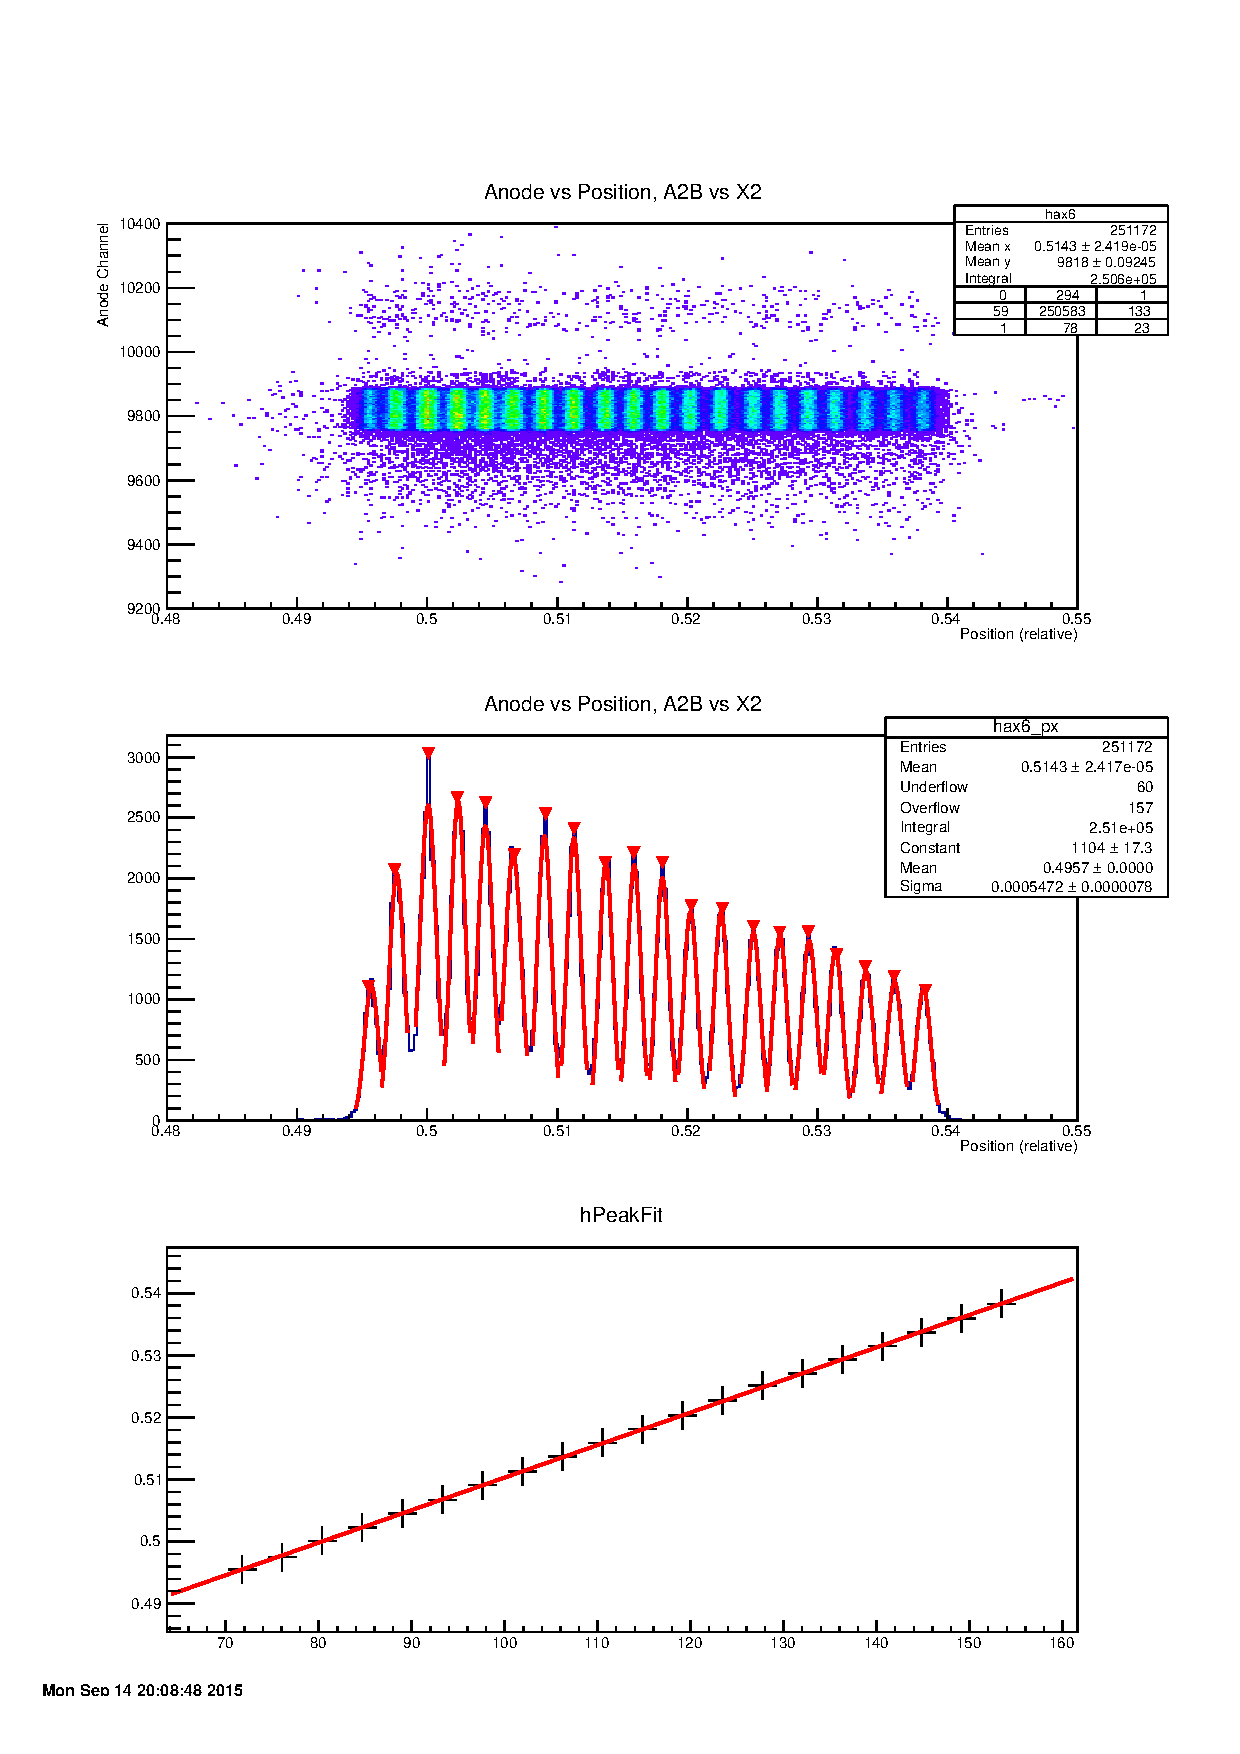
\includegraphics[width=\textwidth,height=0.8\textheight,keepaspectratio]{run_606_peakfit}%
\caption{Illustration of the position calibration technique. The 2D histogram is show in the top panel, in this case it is the $x$-position of detector 2 plotted against the bottom anode signal (also of detector 2). The middle panel shows the $x$-projection of the 2D histogram, that is the $x$-position spectrum gated on anode A2B. The location of the peaks have been identified (the width of the peaks has also been measured). The bottom panel shows how the calibration parameters are generated. The measured positions of the peaks (from the middle panel) are plotted as a function of the known peak positions from Table~\ref{cal2}. A linear fit is applied to the relationship, thus yielding the calibration constants show in Table~\ref{position-calib} for this position-anode combination.
%\enlargethispage{1in}
}%
\label{peakfit}%
\end{figure}

The calibration parameters are determined by comparing the location of the peaks in the spectrum with the known location of the projected features of the mask, which are given in Tables \ref{xpos} and \ref{ypos} (for the April 2014 runs) and in Table~\ref{xpos2} (for the April 2015 runs). As discussed in section \ref{fit}, the position of the peaks in the spectra can be determined using the following routine.
\vsetroot
\begin{quote}
\begin{Verbatim}[firstnumber=0]
peakfitx("hax6","cal/X2_grid.lst")
\end{Verbatim}
\end{quote}
Fig.~\ref{peakfit} shows part of the output of this routine. In the top panel, the 2D histogram \texttt{hax6} is given. 
This is a plot of the anode AB2 signal as a function of the uncalibrated $x$-position. 
The middle panel shows the 1D $x$-projection of the 2D histogram in the top panel. This spectrum, \texttt{hax6\_px}, corresponds to the $x$-position in coincidence with anode AB2. The peaks which have been identified using the subroutine  \texttt{findpeaks()} are indicated by the red triangles and the non-overlapping Gaussian fits determined by the subroutine \texttt{gfindpeaks()} are indicated by the solid red lines. Fig.~\ref{decon} shows a portion of the output from the third step of the peak-finding routine. The fitting range of the first three peaks are shown. As in the middle panel of Fig.~\ref{peakfit}, the peaks found by the subroutine  \texttt{findpeaks()} are indicated by red triangles and the non-overlapping Gaussian fits are indicated by the solid red lines. The global fit calculated by \texttt{decon()} is show by the solid green line. The individual Gaussian fits which make up the global fit are shown by the dashed black lines. By inspection the peak center revealed by the three different techniques is different---in particular for the first peak, located near $x=0.496$.

\begin{figure}
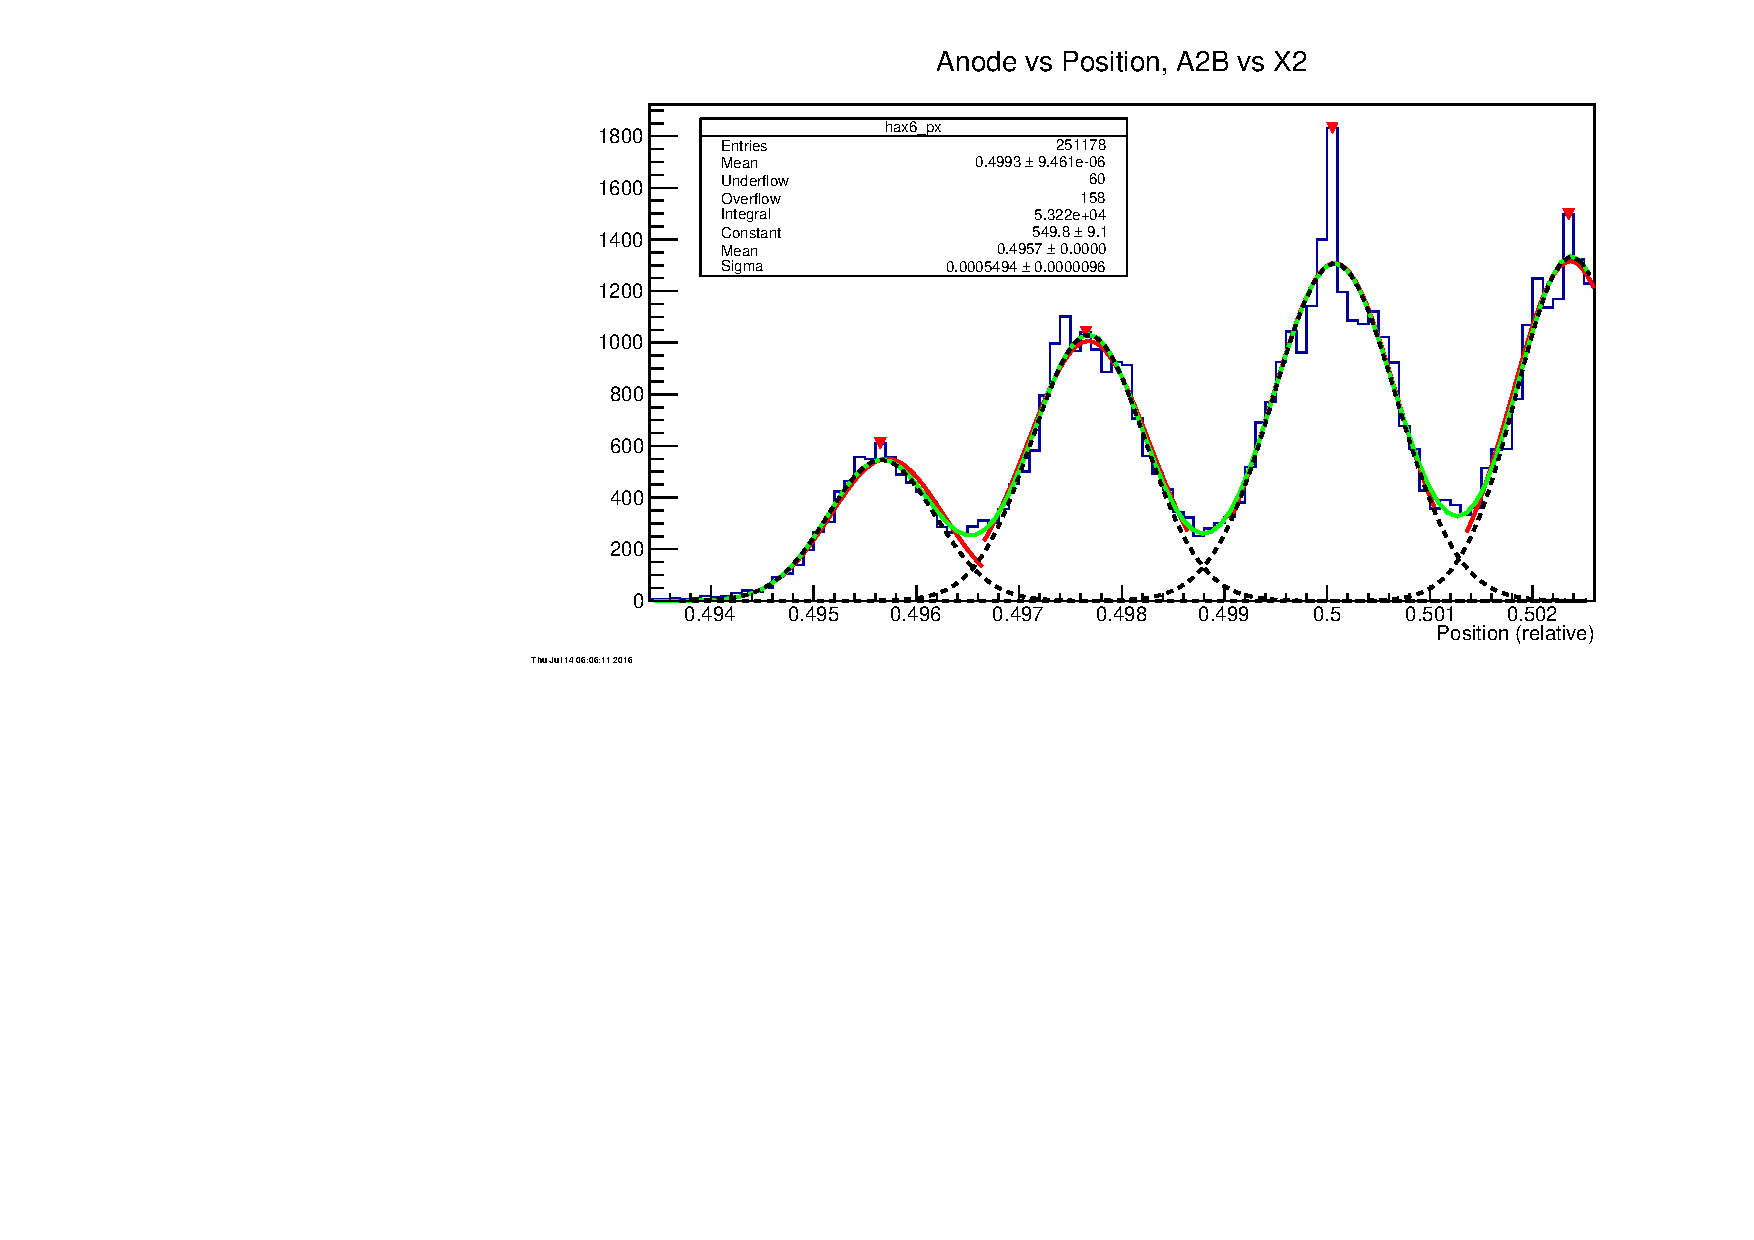
\includegraphics[width=\textwidth,keepaspectratio]{run_606_decon}%
\caption{Illustration of the peak-finding routine used in position calibration.}%
\label{decon}%
\end{figure}

It is the output of the \texttt{decon()} subroutine---that is, the center of the individual Gaussian fits---that are used as the peak positions that are to be calibrated. These positions are plotted on the $y$-axis of the bottom panel in Fig.~\ref{peakfit}. 
The known positions of the peaks are read in from a file, when specified as the second argument of the commands \texttt{peakfit()}, \texttt{peakfits()}, or \texttt{peakfity()}. 
The known positions are plotted on the $x$-axis of the bottom panel in Fig.~\ref{peakfit}. A linear fit is made between these two sets of points, which gives the calibration parameters for the particular andoe-position pair. For convenience, the following command can be used to save the calculated linear fit calibration parameters to file, to be read in during sorting.

\begin{quote}
\begin{Verbatim}[firstnumber=0]
writetemp("cal/run_606_XY.cal",-1,"temp_inv.lst",0,1,1,12,0)
\end{Verbatim}
\end{quote}


The calibration parameters are applied to the uncalibrated data using the code shown in Code Block~\ref{cal-code}. %with the following block of code.
The uncalibrated positions are given by Eq.~\ref{detector_X} with $L=1$ and are therefore unitless.  Naively, the uncalibrated positions should cover the range of 0--1, but inspection of the top  panel in Fig.~\ref{peakfit} shows the rage is closer to 0.49--0.54. In either case, 
the standard fit of the relationship shown in the bottom panel of Fig.~\ref{peakfit} will give calibration parameters  in terms of mm/unit~position.
In these terms, a typical calibration constant would be -0.00119\,mm/unit~position. % with an offset of 0.471\,mm.
 Instead of using calibration constants that are small compared to 1, the inverse of the usual calibration is used, as shown in Code Block~\ref{cal-code}. Typical values for the (inverted) calibration constants are given in Table~\ref{position-calib}.
\vspace{0.5\baselineskip}
\par\noindent
\begin{minipage}{\linewidth}
\singlespace
\begin{lstlisting}[caption={Position calibration procedure. The index \texttt{i} runs over 3--6, corresponding to each of the four positions. Each position has a separate set of calibration parameters for each anode segment. The calibration parameters are stored in the array $12\times2$ \texttt{hxcal[][]}. Typical calibration parameters are given in Table~\ref{position-calib}.},label={cal-code}]
for(int k=0;k<3;k++) {
  if(a[k+3*(int)((i-3)/2)][1]>0)
    x[i-3][1]=(x[i-3][0]*hxcal[((i-3)*3)+k][0])+hxcal[((i-3)*3)+k][1];
}
\end{lstlisting}
\end{minipage}

\begin{table}
\centering  
\begin{tabular}{c..}
\hline
\multicolumn{1}{c}{Pair}& \multicolumn{1}{c}{Slope}& \multicolumn{1}{c}{Offset} \\
\multicolumn{1}{c}{\texttt{i}}&\multicolumn{1}{c}{\texttt{hxcal[i][0]}}&\multicolumn{1}{c}{\texttt{hxcal[i][1]}}\\ \hline \hline
 0 & 1878.17 & -864.607 \\
 1 & 1851.11 & -851.023 \\
 2 & 1875.96 & -863.33 \\
 3 & 1734.11 & -843.706 \\
 4 & 1633.01 & -790.65 \\
 5 & 1645.94 & -794.028 \\
 6 & 1919.17 & -879.249 \\
 7 & 1905.22 & -872.308 \\
 8 & 1909.97 & -874.645 \\
 9 & 1783.57 & -867.804 \\
10 & 1620.39 & -784.588 \\
11 & 1586.56 & -764.344 \\
 \hline 
\end{tabular}
\caption{Typical calibration constants for each of the twelve possible anode-cathode pairs (\texttt{i}). Parameters are given for run 606. 
%can be correlated with each of the three anode segment pairs (\texttt{k}); twelve combinations in total. The index runs from 0--11 and is defined by $(\texttt{i}-3)\times 3 + \texttt{k}$.
}
\label{position-calib}
\end{table}





%\subsection{Simulations}
A Monte Carlo simulation has been constructed to study the various contributions to the measured resolution.  An example output is shown in Fig.~\ref{sims}. To produce the figures discussed in this section, the simulation included a uniform spherical scattering distribution and a finite beam spot.  Specifically, the beam spot has been simulated as a symmetric Gaussian distribution with 90\% of the beam falling within a radius of $\rho=1.0$\,mm ($\sigma = 0.608$\,mm). This beam spot size was selected to be conservatively large and yet physically reasonable.
\subsubsection{Contributions}
One of the purposes of studying the detector via a simulation was to deconvolve the various contributions to the detector resolution. The results of the simulation study indicate that the observed detector resolution is dominated by the intrinsic detector resolution.  As discussed in Section~\ref{cal_def}, the contribution of the transverse extent of particle trajectories is less than 170\,$\mu$m at the edges of the detector. Near the center of the detector, the contribution approaches zero. These effects are neglected in all of the simulations.

To isolate the contribution of the beam spot size, simulations were run neglecting the effects of beam scattering and detector resolution. Fig.~\ref{sims} shows the simulated position spectra from detector 2.  Comparing Fig.~\ref{sims} with Fig.~\ref{hxc}, one sees that the beam spot size has a minimal contribution to the measured detector resolution. This is not surprising given the distance between the target and the detectors (682.9\,mm) and reasonably-assumed size of the beam spot (1--2\,mm). In order to reproduce the observed resolution in Fig.~\ref{hxc} from the contribution of the beam spot alone, physically unrealistic beam spot sizes are required. For example, a beam spot greater than the size of the target foil is required.
\begin{figure}%
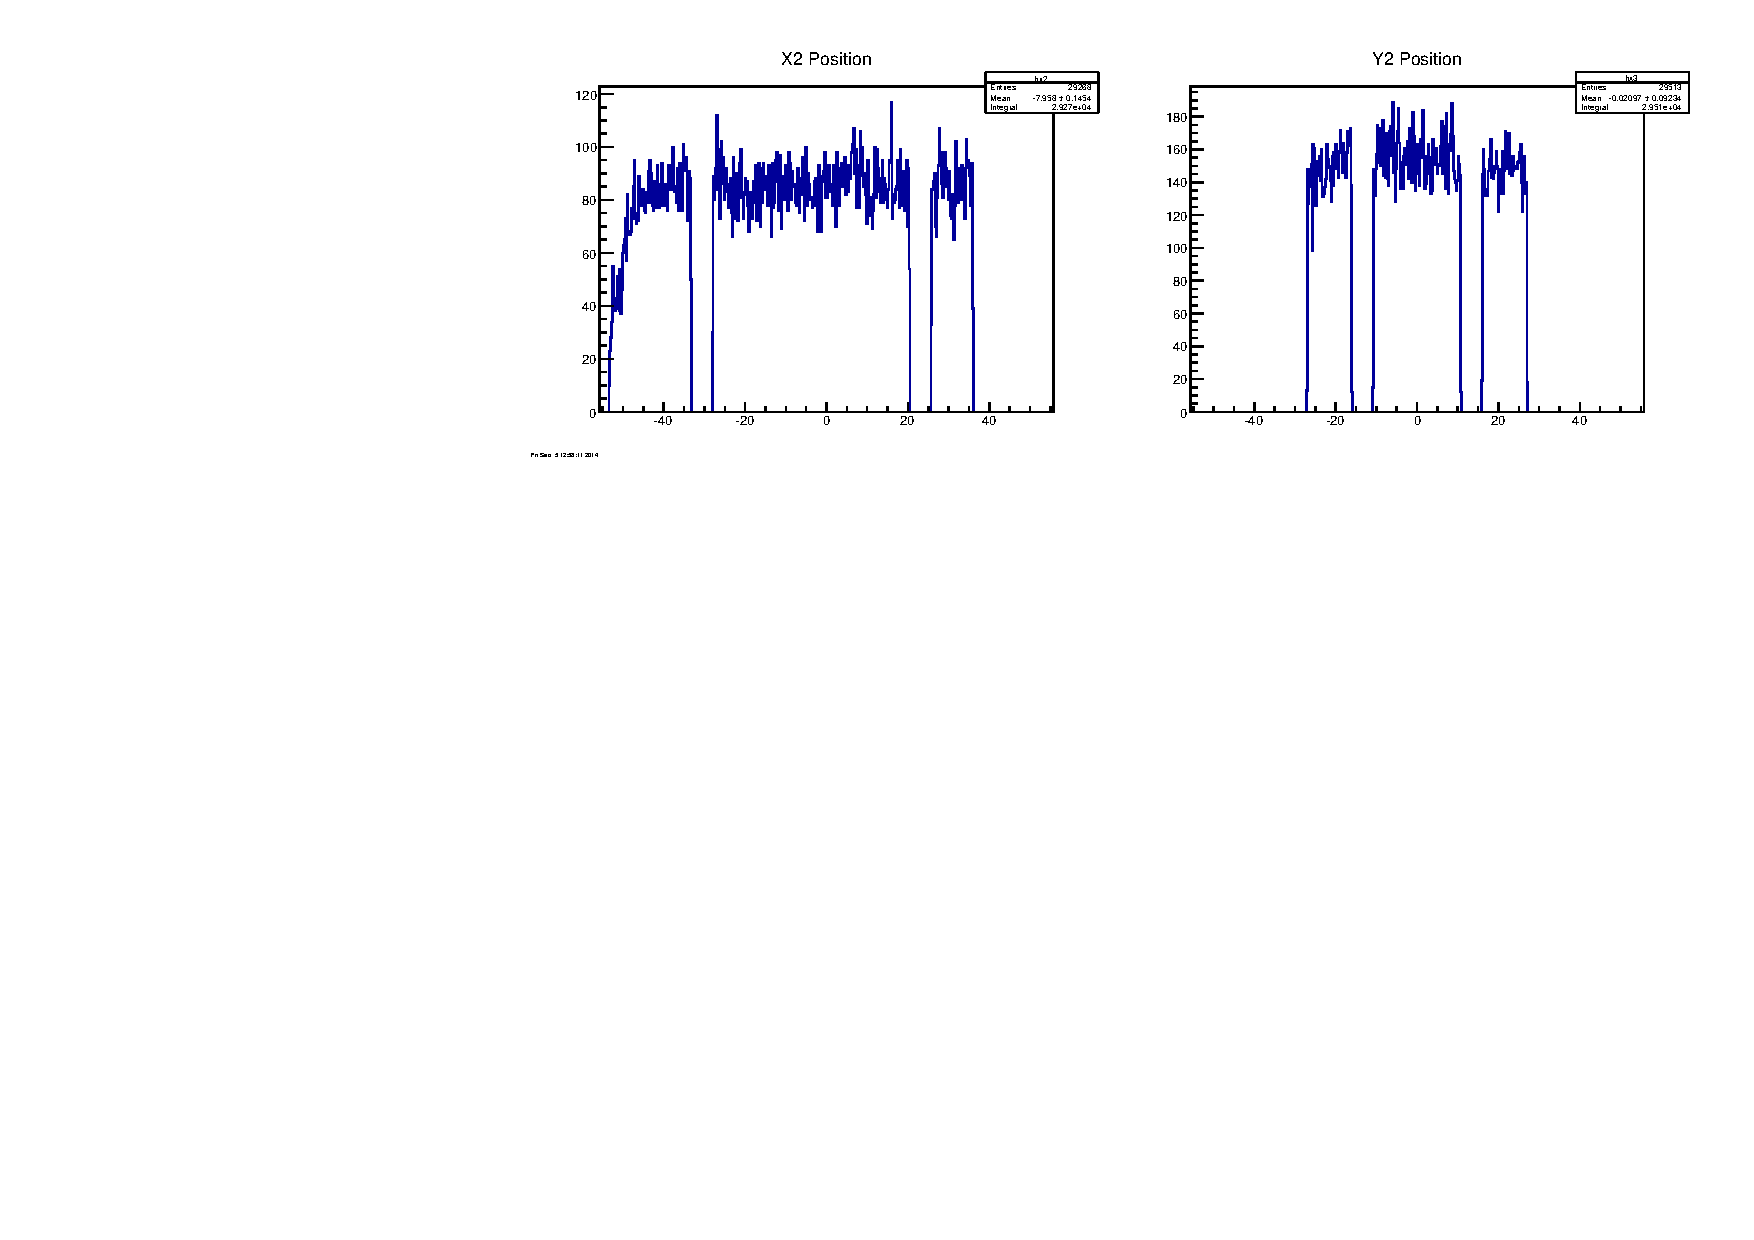
\includegraphics[width=\columnwidth]{sims}%
\caption{Simulated positions spectra of detector 2.}%
\label{sims}%
\end{figure}

\subsubsection{Fitting the Data}
The determination of the detector resolution is accomplished by fitting the data with the simulation. The position of the beam spot is accounted for by geometrically aligning the features of the simulation with those the data. Once the simulation is aligned to the data, the measurement resolution of the simulation is varied to match the shape of the data. Fig.~\ref{sim_comp} show the result of fitting the data with the simulation in order to determine the position resolution of the detector. Because the simulation adequately reproduces the data without including edge scattering, implementation of that effect is neglected. In this example, the data was best fit with a simulated intrinsic detector resolution of 1.3\,mm (3.06\,mm~FWHM).  This fit is consistent with the dubious edge-fitting method presenting in the previous section. For an example such as this, where the wires are not resolved, the quality of the fit of the simulation could be improved on the order of 8\% by including a realistic angular distribution.
\begin{figure}%
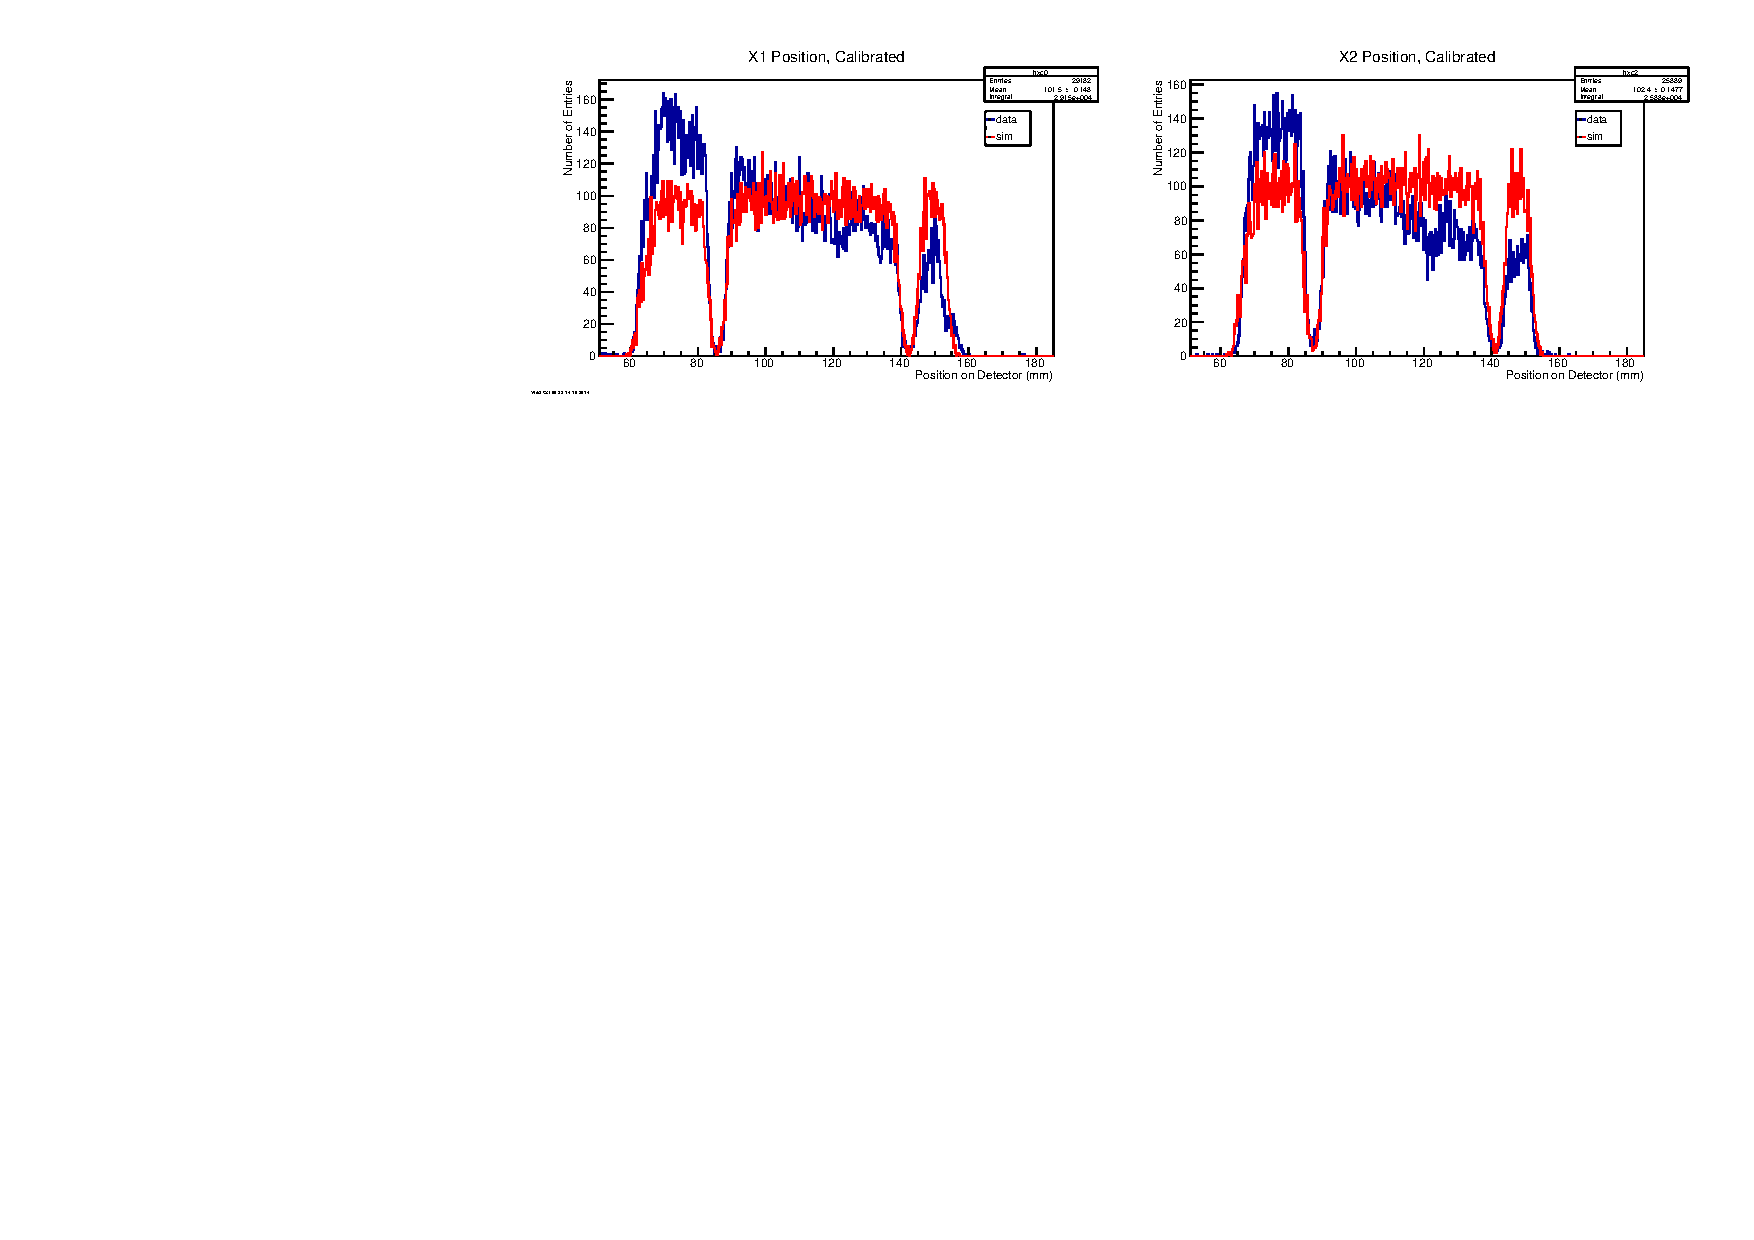
\includegraphics[width=\columnwidth]{run_480_compX}%
\caption{Simulated and measured $x$-position spectra of for each detector. The data (blue) have been fit with a simulated spectra using the following assumptions: a 1.43\,mm~FWHM beam spot centered at the origin and a detector resolution of 1.3\,mm (3.06\,mm~FWHM).}%
\label{sim_comp}%
\end{figure}



\section{Results}
\subsection{Data Selection}
\subsubsection{Data}
The 2014 experiment started on \longusdate\formatdate{25}{4}{2014} with Run 371 and ended on \longusdate\formatdate{28}{4}{2014} with Run 480. This yields 110 runs. However, not all of the data was written to disk. Data was written to disk for 69 runs.

The 2015 experiment started on \longusdate\formatdate{21}{4}{2015} with Run 576 and ended on \longusdate\formatdate{23}{4}{2015} with Run 611. This yields 36 runs.  Data was written to disk for 24 runs. They first day of testing involved shake-down of the detector and acquisition system. The two runs from that day have variable gain and are excluded.
\subsubsection{Amplification}
The difference of each pair of anode signals and the sum of each pair of cathode signals are expected to be sharply peaked. There are three pairs of anodes, but the TDC data only includes the logical \texttt{OR} of the anode signals, so only one ``pair'' is present. Each of the four positions is represented by a pair of cathode signals. The data was assessed by measuring what fraction of the data fell under a $\pm 2 \sigma$ gate around the tallest peak in each of the five spectra. The five fractions were added together to create a single assessment parameter. Fig.~\ref{hsumz} shows an example of this technique. Assessing the data in this manner, the data runs fall into two groups. Those with sharpness parameter below 2.8 (average 2.4) and those with a sharpness parameter over 3.6 (average 4.2).

\begin{figure}[ht]
\centering
\hspace{\fill}
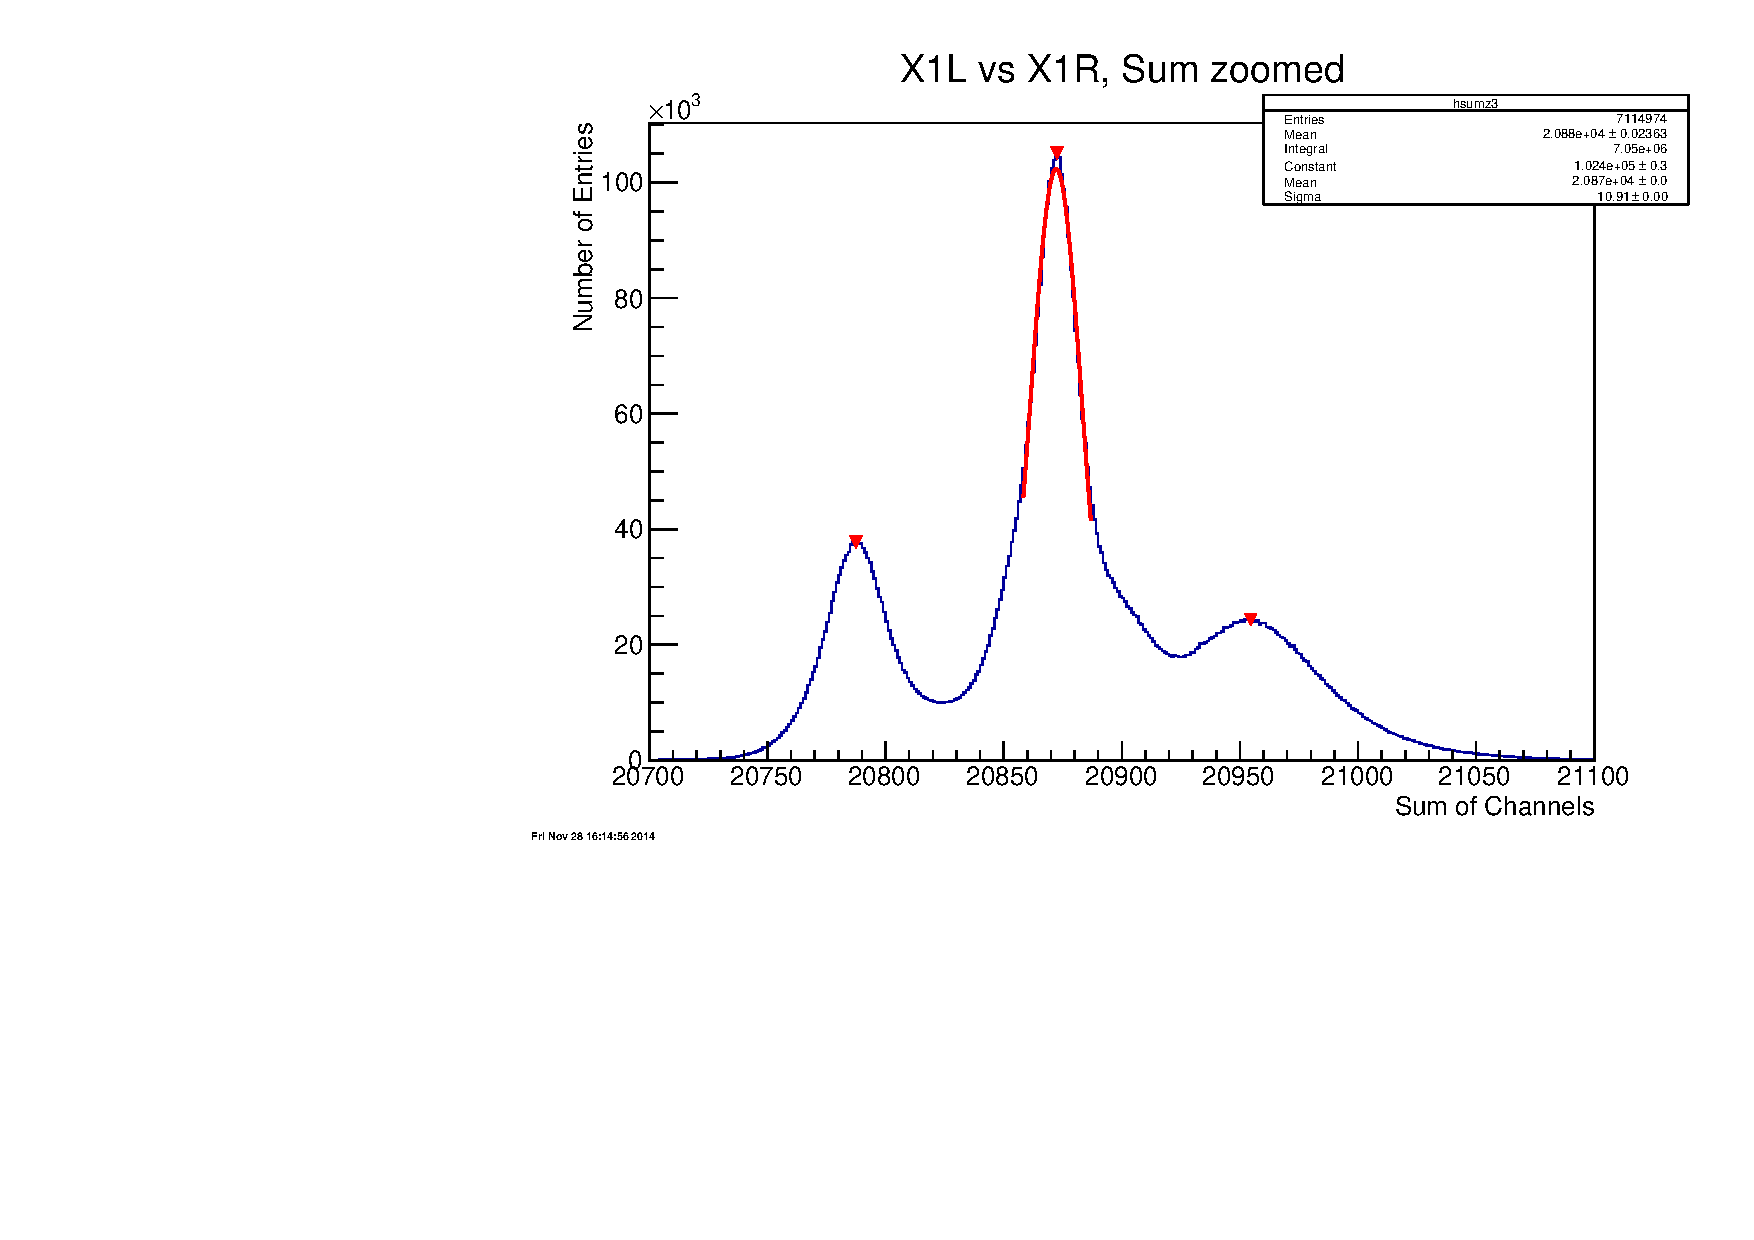
\includegraphics[width=0.48\textwidth, keepaspectratio]{run_430_hsumz3}\hspace{\fill}
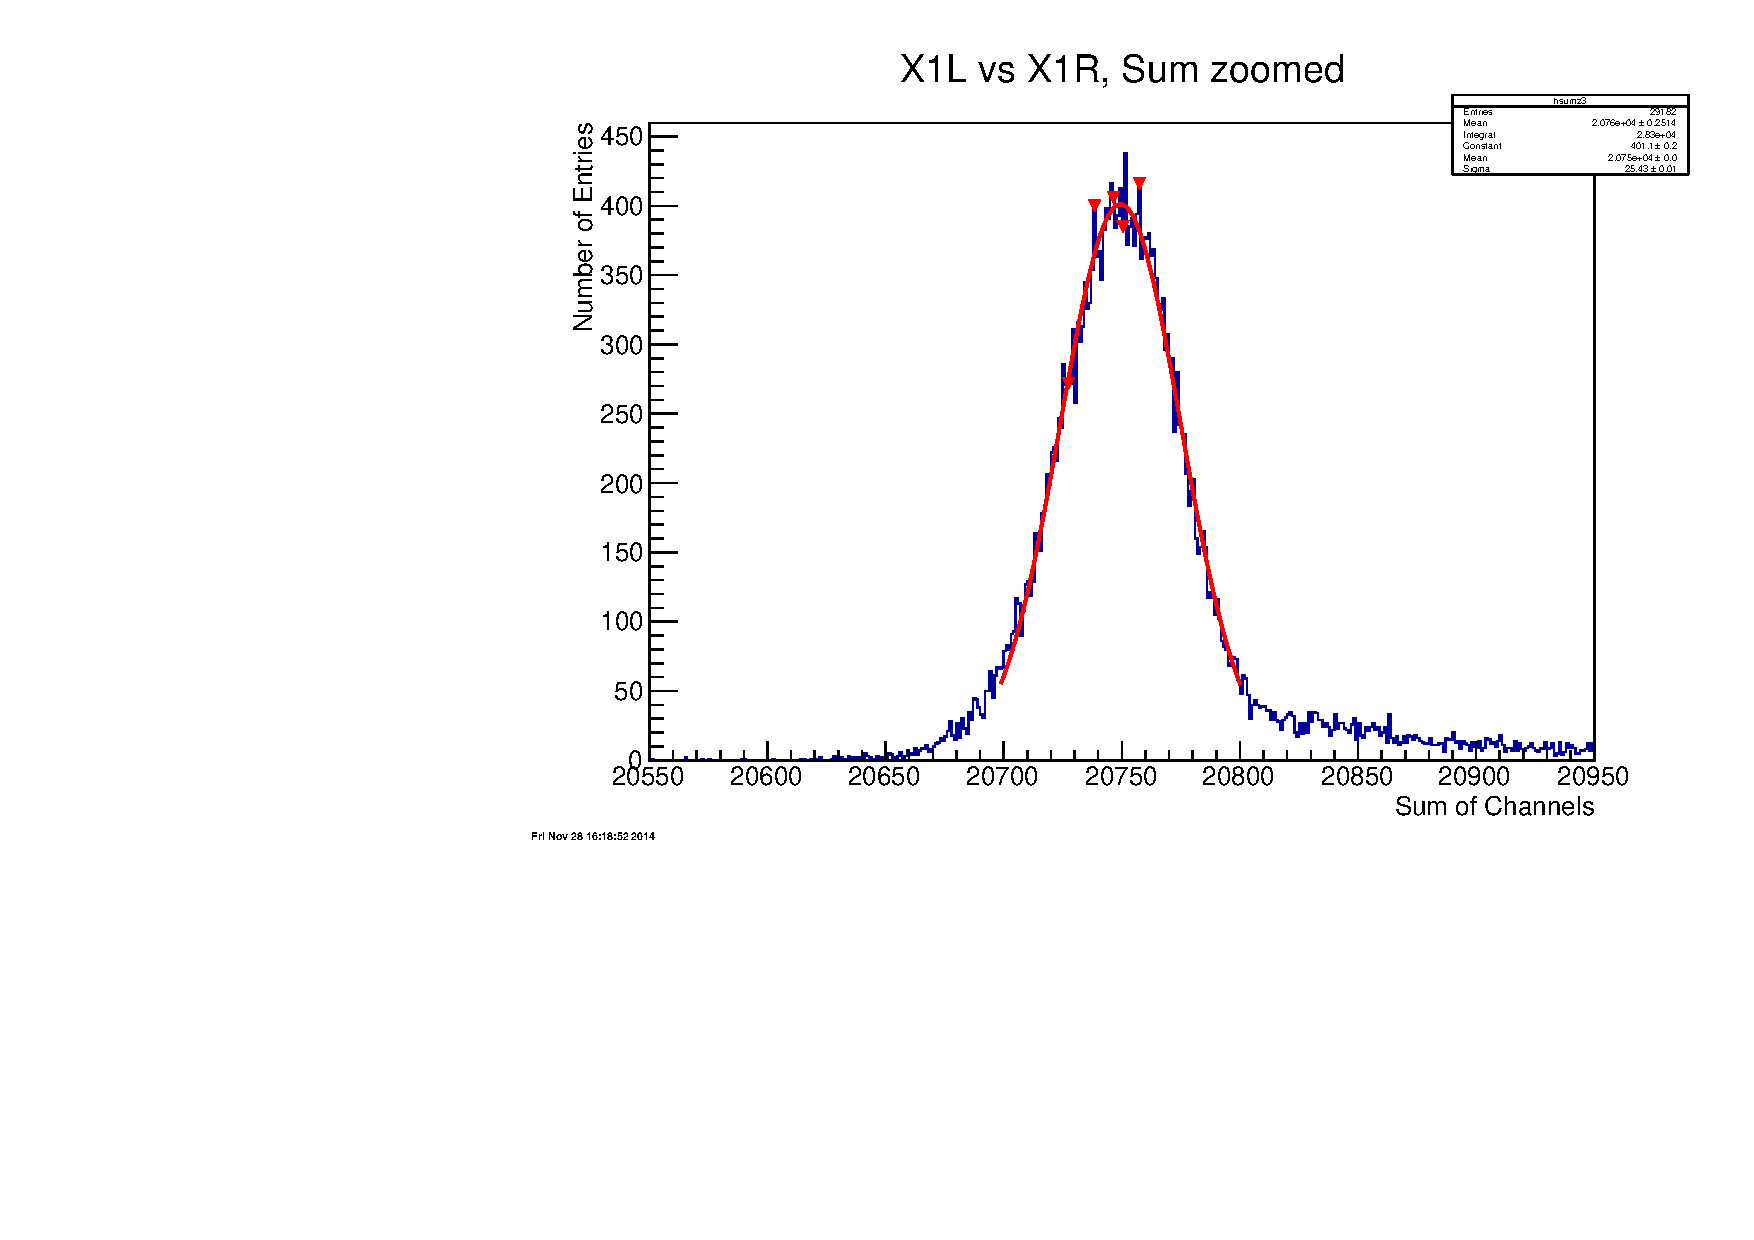
\includegraphics[width=0.48\textwidth, keepaspectratio]{run_480_hsumz3} \hspace{\fill}
\caption{Example cathode sum spectra for Run 430 (left) and Run 480 (right). In both figures, the sum of X1L and X1R is plotted over 400 channels. In Run 430, the sum spectra is divided into three peaks with 47\% of the data falling within $\pm 2 \sigma$ of the tallest peak. In Run 480, all of the data falls into a single peak with 83\% of the data falling within $\pm 2 \sigma$.}
\label{hsumz}
\end{figure}

Selecting the data based on this sharpness parameter is supported by examining the correlation between the difference in anode signals versus the sum of the various cathode channels. Such a plot is shown in Fig.~\ref{htsum}. All of the data with a sharpness parameter less than 2.8 correspond to data before Run 437. Referring to \S\ref{amp-settings}, one see that this corresponds to those runs which had a $10\times$ lower signal amplification at the input of the level discriminator and thus had higher peak-to-threshold ratio. Rejecting the data before Run 437 leaves 39 data runs.

\begin{figure}[ht]
\centering
\hspace{\fill}
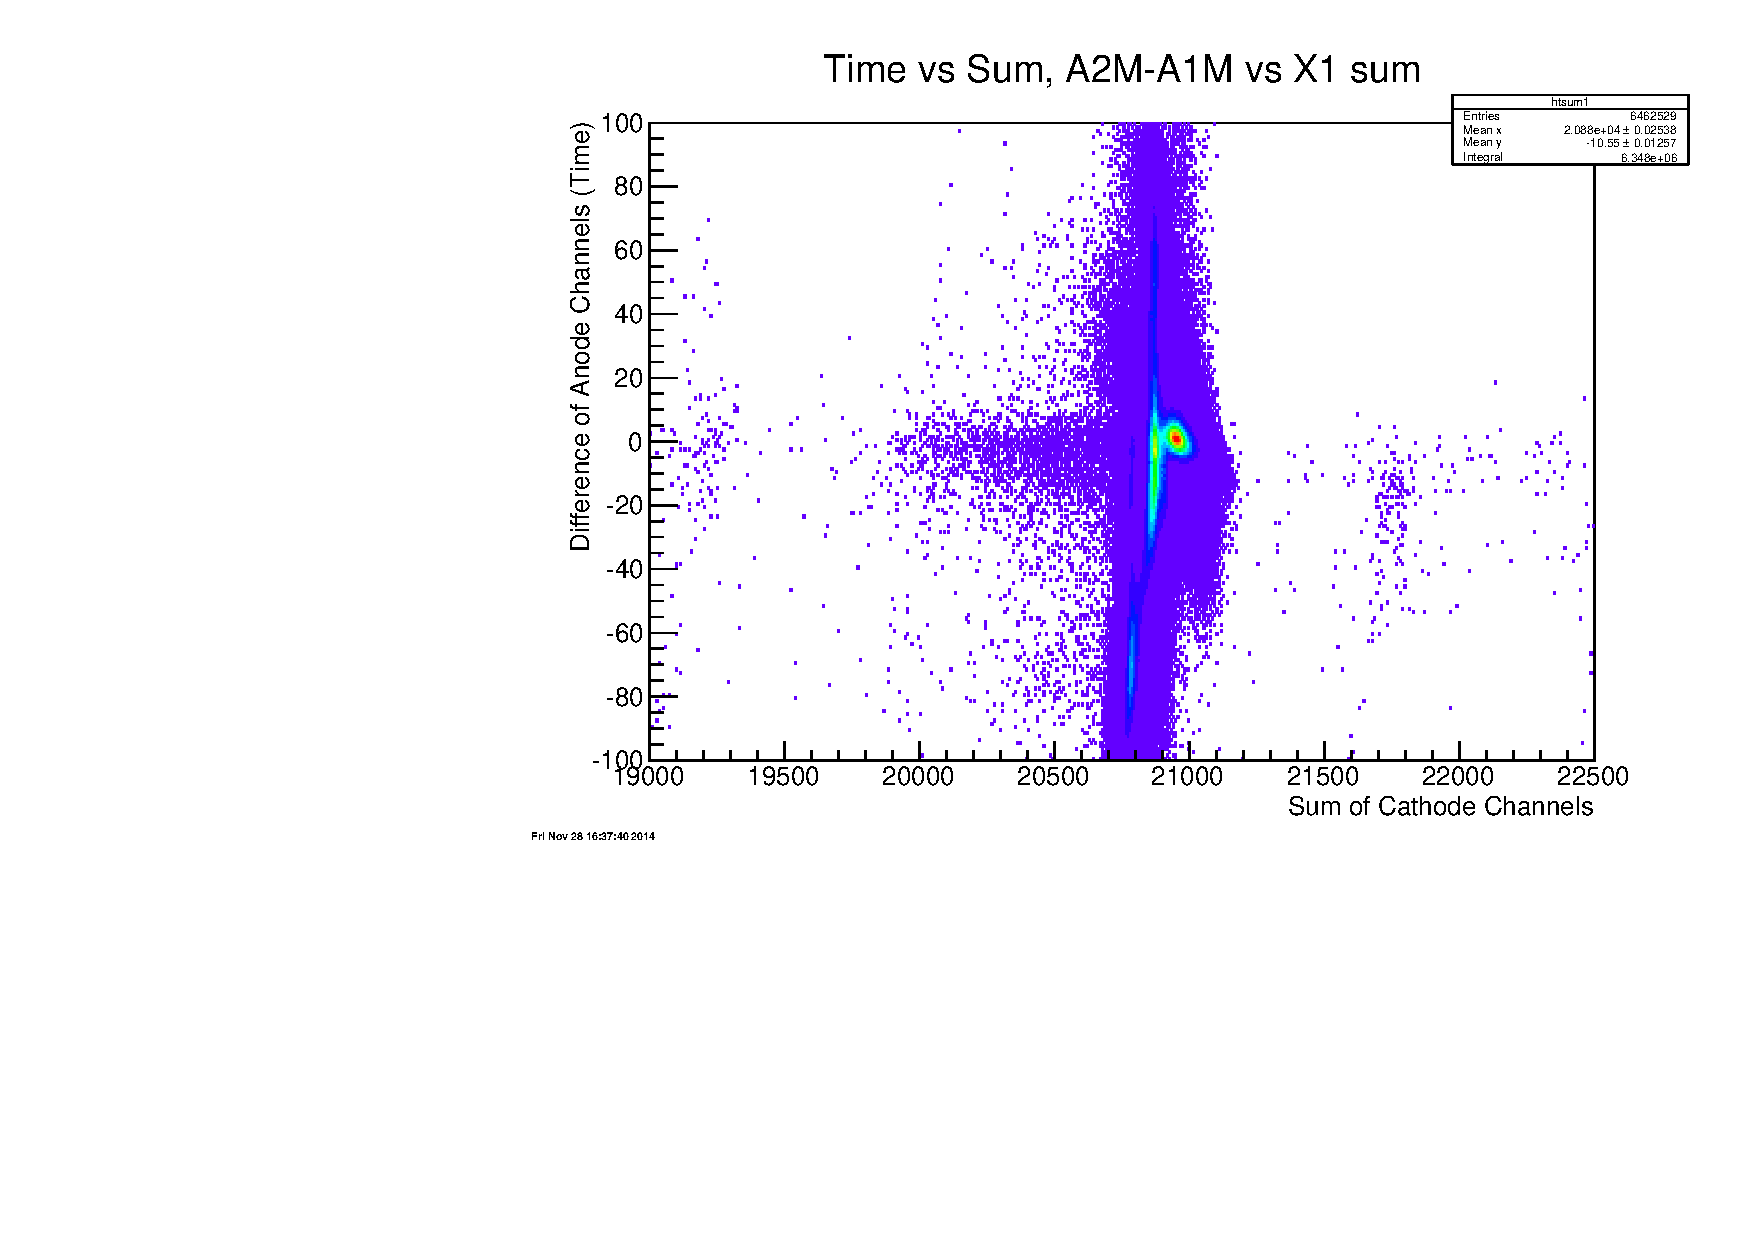
\includegraphics[width=0.48\textwidth, keepaspectratio]{run_430_htsum1}\hspace{\fill}
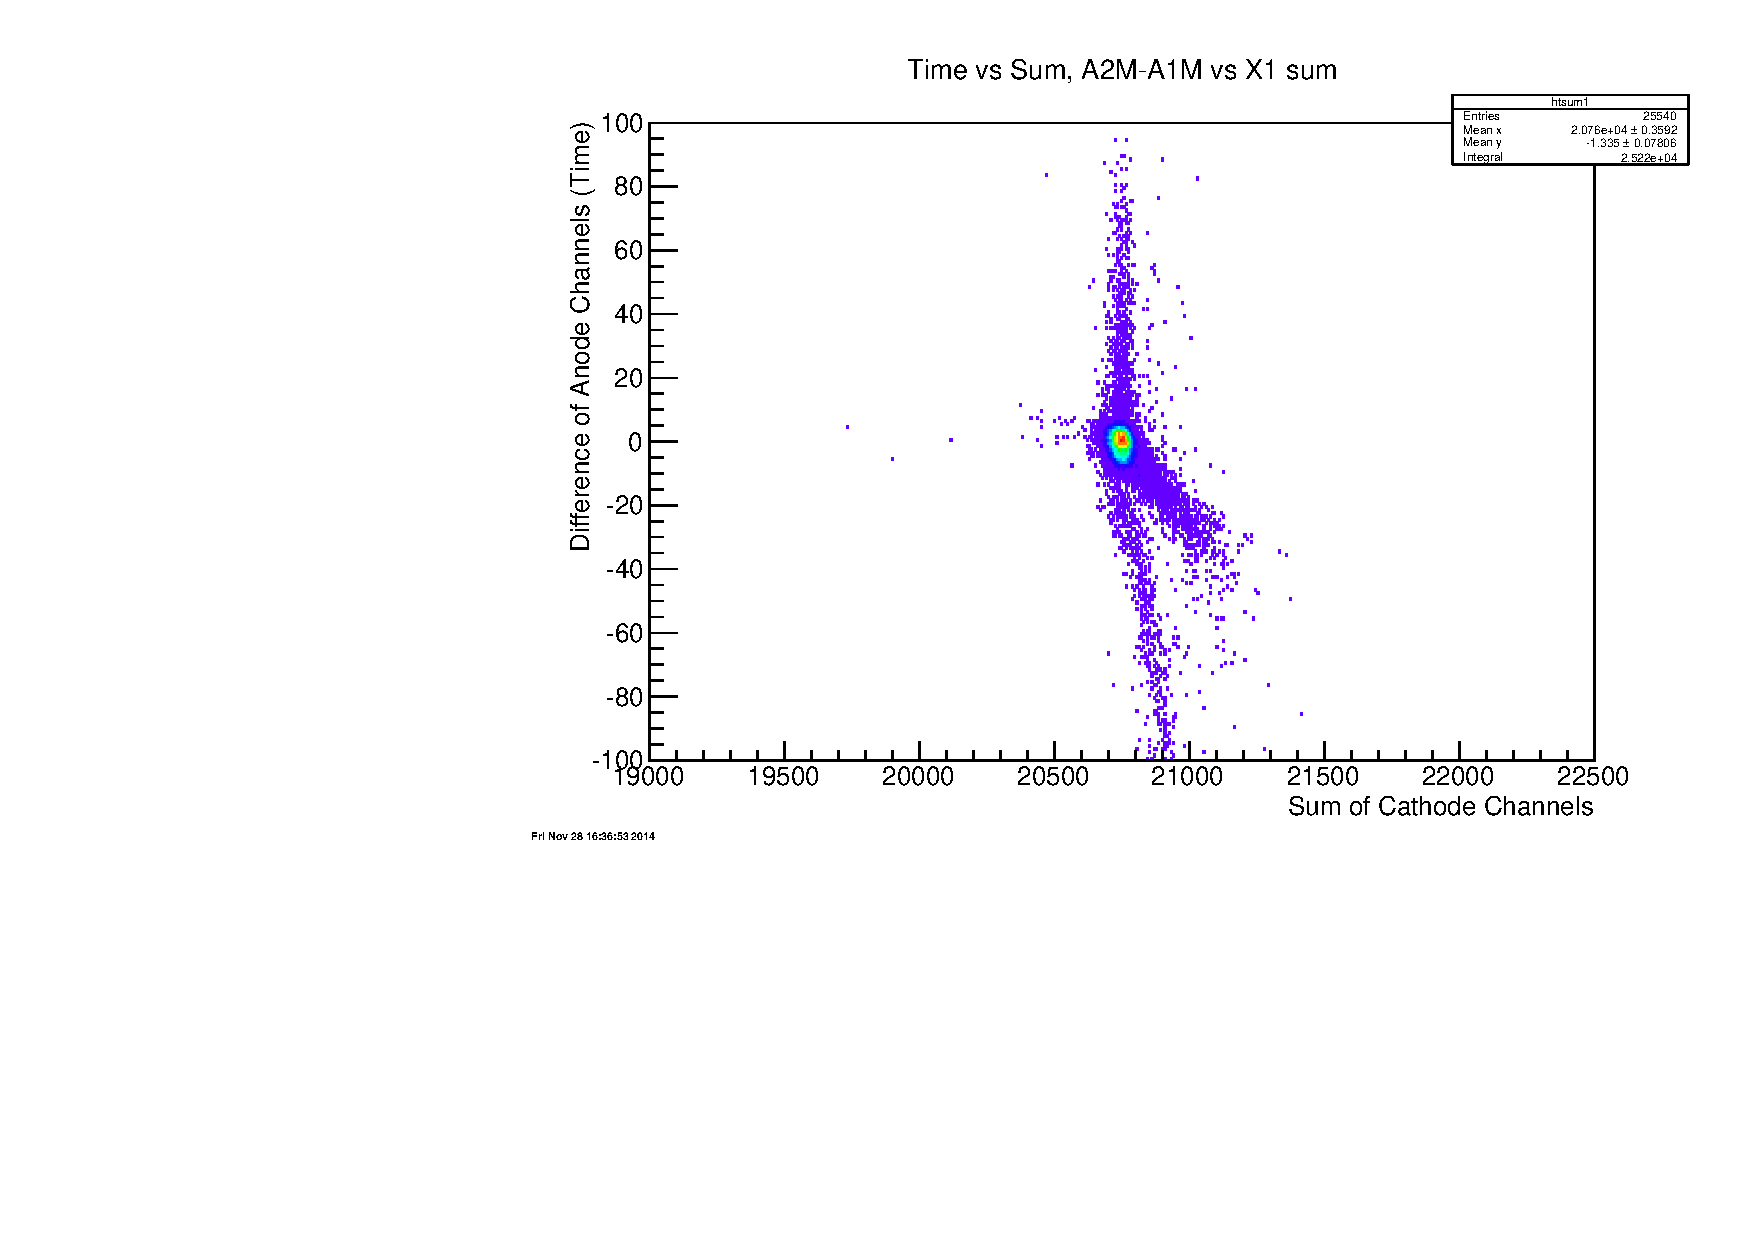
\includegraphics[width=0.48\textwidth, keepaspectratio]{run_480_htsum1} \hspace{\fill}
\caption{Example anode difference (time) vs cathode sum spectra for Run 430 (left) and Run 480 (right).}
\label{htsum}
\end{figure}

\subsubsection{Trigger rate}
Examining the trigger rate of the data runs further divides the data into two groups. The effective trigger rate was determined by measuring the number of anode coincidences and dividing by the duration of the run in seconds. 
\paragraph{2014 Test}
The data runs which used the digitizer 
%Most of the data runs 
had trigger rates less than 410 anode coincidences per second (74\,cps average). 
The data runs that did not use the digitizer %However, a number of the data runs 
had significantly higher trigger rates: over 2,000\,cps (7,400\,cps average). The data may be similarly divided based on the data rate.
%A number of the runs have data rates of 
Despite the higher event rate, the runs which did not use the digitizer have a lower data rate: 
less than 0.8\,MB/s (0.63\,MB/s average). 
The run which used the digitizer 
%Most of the runs 
have data rates greater than 3.4\,MB/s (10.1\,MB/s average). 

Excluding the non-digitizer runs, those runs with high trigger rates and low data rates, leaves 30 candidate data runs to assess the detector performance. The justification for this exclusion is explained in the next section. At the time of analysis, the  digitizer settings were not properly associated with their corresponding data runs. Therefore, it was unclear what the source of the varying data rates was.
\paragraph{2015 Test}
Most of the runs were without the digitizer enabled. The data rate for these runs was 89\,kB/s. With the digitizer enabled, the average data rate was 8.2\,MB/s. Unlike the 2014 test, the runs without the digitizer have excellent data. None of the pathological structures discussed in the previous section or the following section are present. This is likely due to proper triggering and optimized thresholds.

\subsubsection{Structure (2014 Test)}
The data from the high count rate (or low data rate) runs has some unusual structural features. For example, the results of the position calibration for detector 1 are shown in Fig.~\ref{overlay}. This data is from Run 430 and is generated with the following command.
\vsetroot
\begin{quote}
\begin{Verbatim}[firstnumber=0]
grantplot()
\end{Verbatim}
\end{quote}
\vsetnone
 The settings for this run are $P=3$\,Torr, $V_\textrm{c}=-75$\,V, $V_\textrm{a}=+420$\,V ($\Delta V=495$\,V). The beam current for this run was 4.24\,enA ($10\times$ attenuator). In the figure, the calculated projected positions of the mask features (red lines) and the positions of the Kapton shields (blue lines) have been overlaid with the data. The calculated positions of the calibration features are in good agreement with the data, indicated that the data has been properly calibrated. 

\begin{figure}
\centering
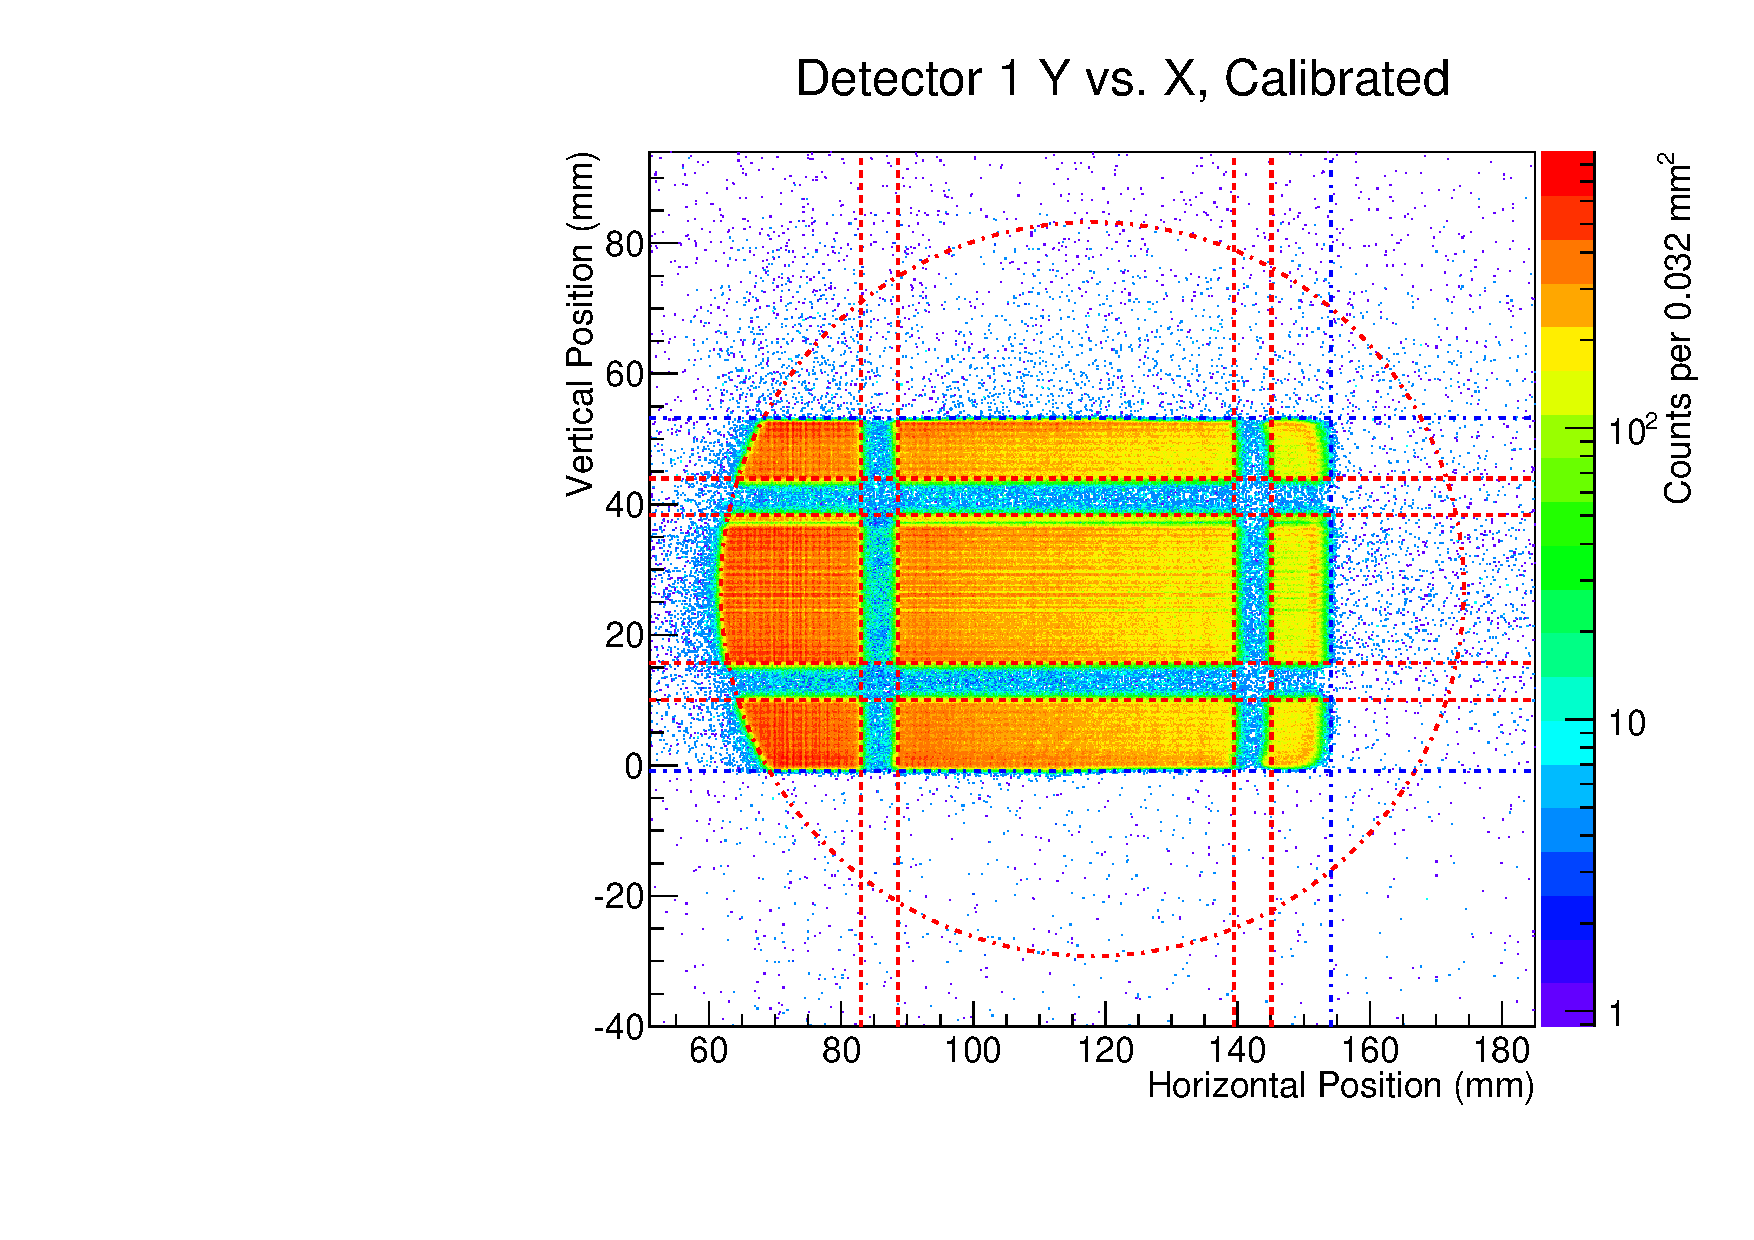
\includegraphics[width=\columnwidth,height=0.33\textheight,keepaspectratio]{run_430_hhitc0_overlay_c_log2z}%
\caption{Calibrated position spectrum for detector 1.  The calculated projections of the mask aperture (red dash-dotted line) and mask features (red dashed line) are plotted. The boundary of the fiducial area, corresponding to the location of the Kapton shields is also shown (blue dash-dotted line). Data from Run 430.}%
\label{overlay}%
\end{figure}

The wire grid of the cathodes is visibly resolved.  %demonstrating 
At first glance, this  would suggest that the detector resolution is $\lesssim 1$\,mm~FWHM. 
Fig.~\ref{peaks} shows a portion of the $y$-projection of Fig.~\ref{overlay}. The peaks have been fit and indicated with red arrows; the average gap between the peaks is 0.96\,mm. The width of the last peak is 0.47\,mm or 1.10\,mm~FWHM. This estimate of the resolution is borne out by the simulations as shown in Fig.~\ref{sim_comp2}. This figure is generated with the following macro in \texttt{load\_and\_plot.cc} which requires the PGAC simulation package \texttt{generator.cc}.
\vsetroot
\begin{quote}
\begin{Verbatim}[firstnumber=0]
resplot()
\end{Verbatim}
\end{quote}
\vsetnone
This behavior---that is, the resolution of the wire grid---is %typical of the detector and is
 visible at all pressures that were measured (2, 3, 4, and 6\,Torr). %It remains for the author to assess the dependence and variation of the detector resolution with the detector settings. 
The resolution of the \textit{anode} wires may be expected in the $y$-direction, however, inspection of Fig.~\ref{overlay} shows that resolution of a 1\,mm structure is present in both the $x$- and $y$-directions. The presence of the peaks in the $x$-direction makes this data suspect. This data is excluded by the trigger rate selection detailed in the previous section. This exclusion is justified by the trajectory analysis presented in the following section.
\begin{figure}
\centering
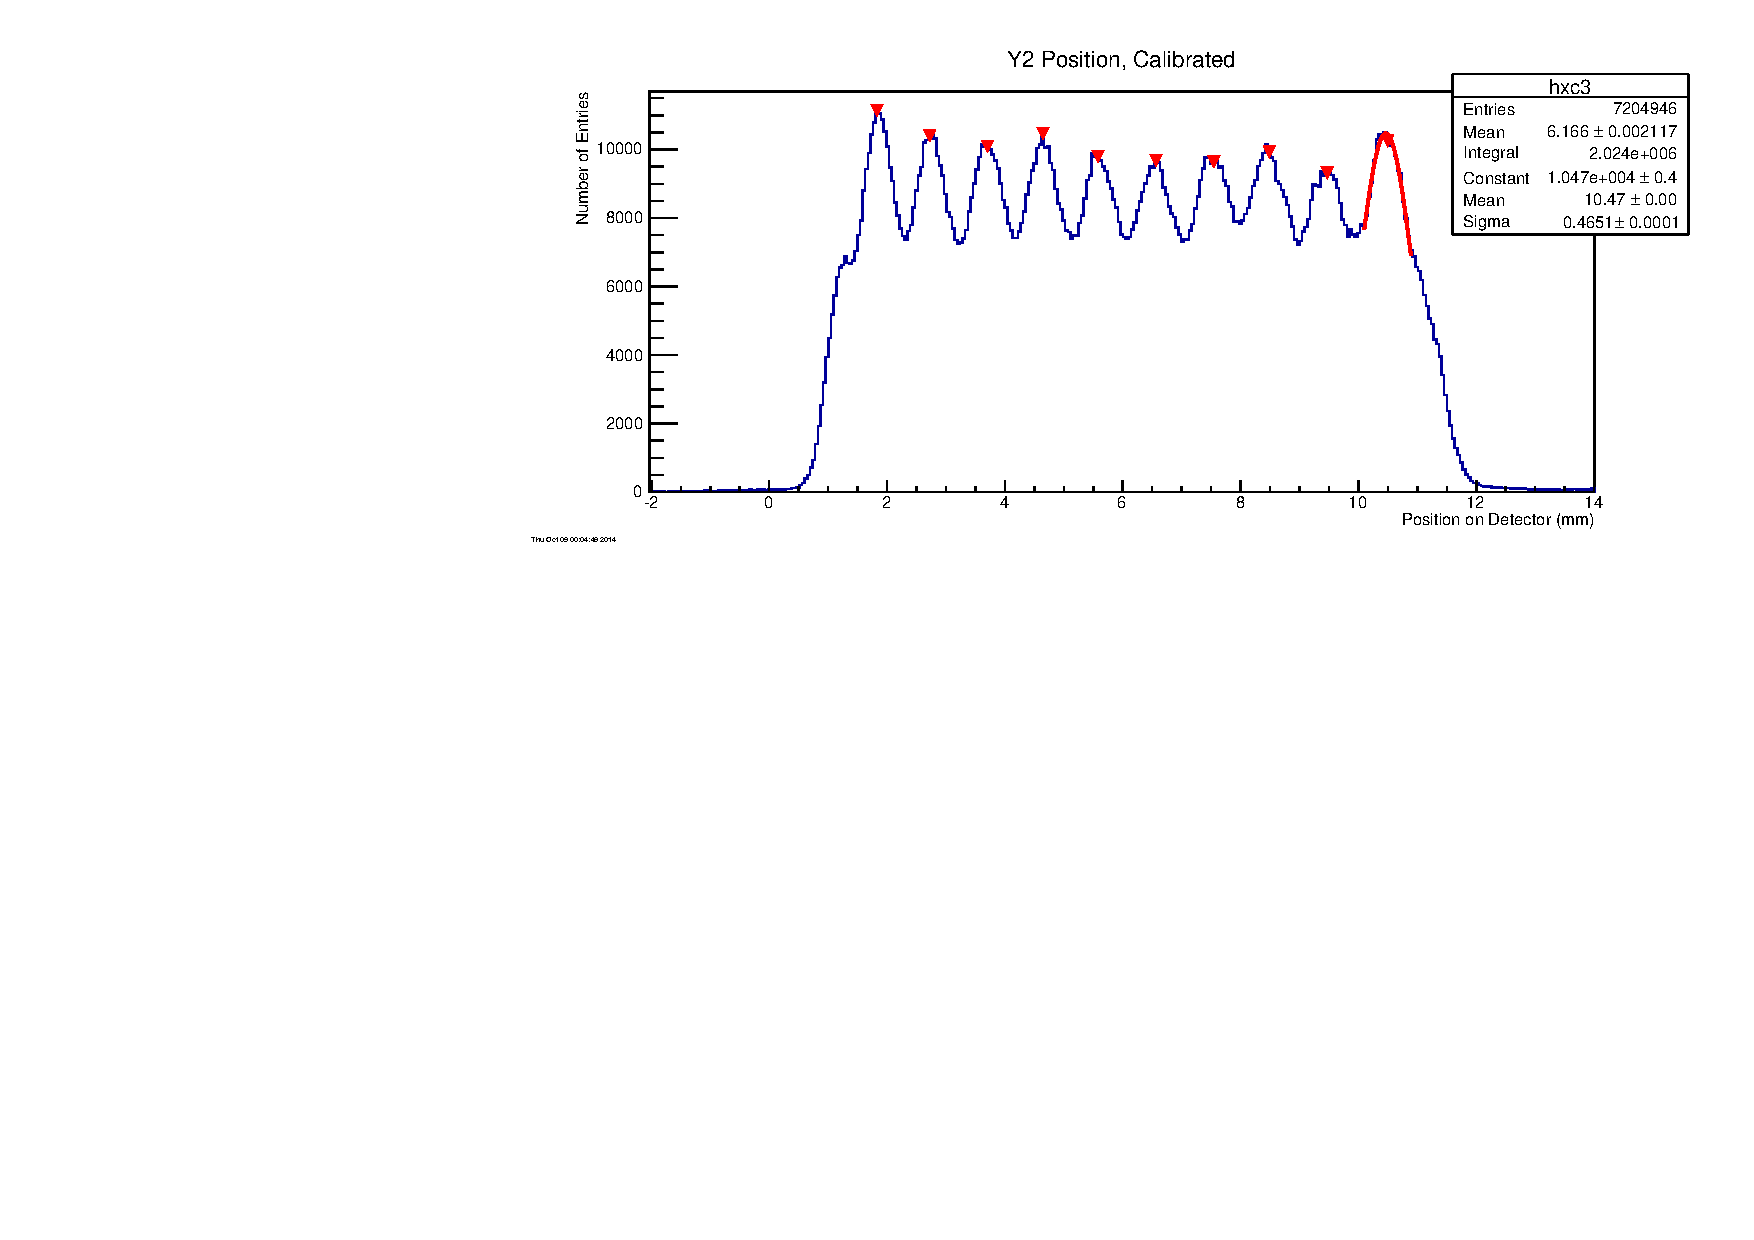
\includegraphics[width=\columnwidth,height=0.33\textheight,keepaspectratio]{run_430_hxc3}%
\caption{Example position spectrum showing the resolution of the cathode wires. The peaks have been identified and their positions are marked with red triangles. The last peak has been fit with a Gaussian for reference. This data is a portion of the $y$-projection ƒof Fig.~\ref{overlay}. Data from Run 430.}%
\label{peaks}%
\end{figure}

\begin{figure}%
\centering
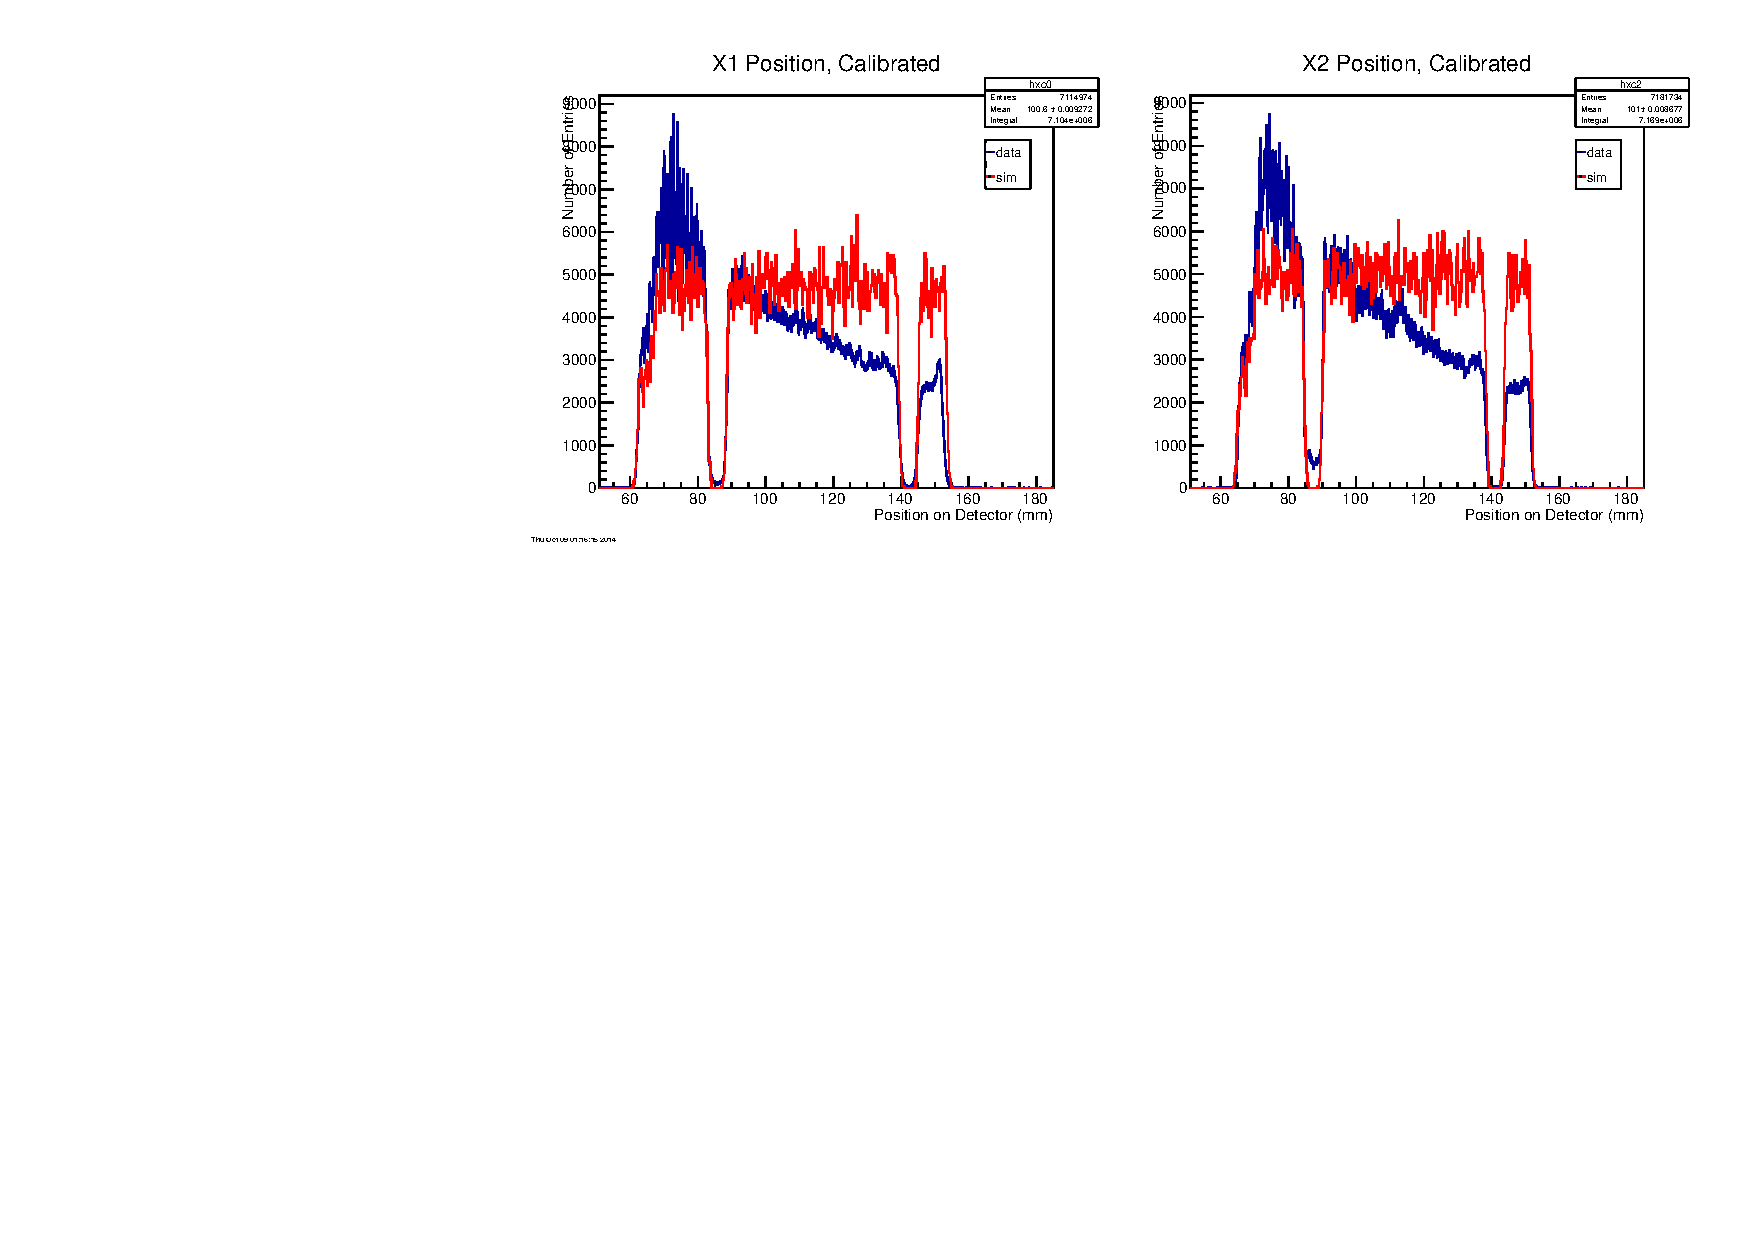
\includegraphics[width=\columnwidth,height=0.33\textheight,keepaspectratio]{run_430_compX}%
\caption{Simulated and measured $x$-position spectra of for each detector. The data (blue) have been fit with a simulated spectra using the following assumptions: a 1.43\,mm~FWHM beam spot centered at the origin and a detector resolution of 0.43\,mm (1.10\,mm~FWHM). Data from Run 430.}%
\label{sim_comp2}%
\end{figure}
\subsubsection{Trajectories}
Given the narrow trajectories incident to the detector---$\pm2.3^\circ$ in the $y$-direction and $-4.5^\circ$--3.0$^\circ$ in the $x$-direction---a strong correlation is expected between the position on each detector. Fig.~\ref{hxxc} shows the $x$-direction on detector 1 plotted as a function of the $x$-direction on detector 2; similarly for the $y$-direction. For Run 480 (bottom panel), the data form a single locus of points with a strong correlation between the detectors. The data from Run 430 (top panel) is characteristic of the high trigger rate runs. The expected locus of points is present, however, it is sitting on top of a background of variable gain and random correlation.

\begin{figure}
\centering
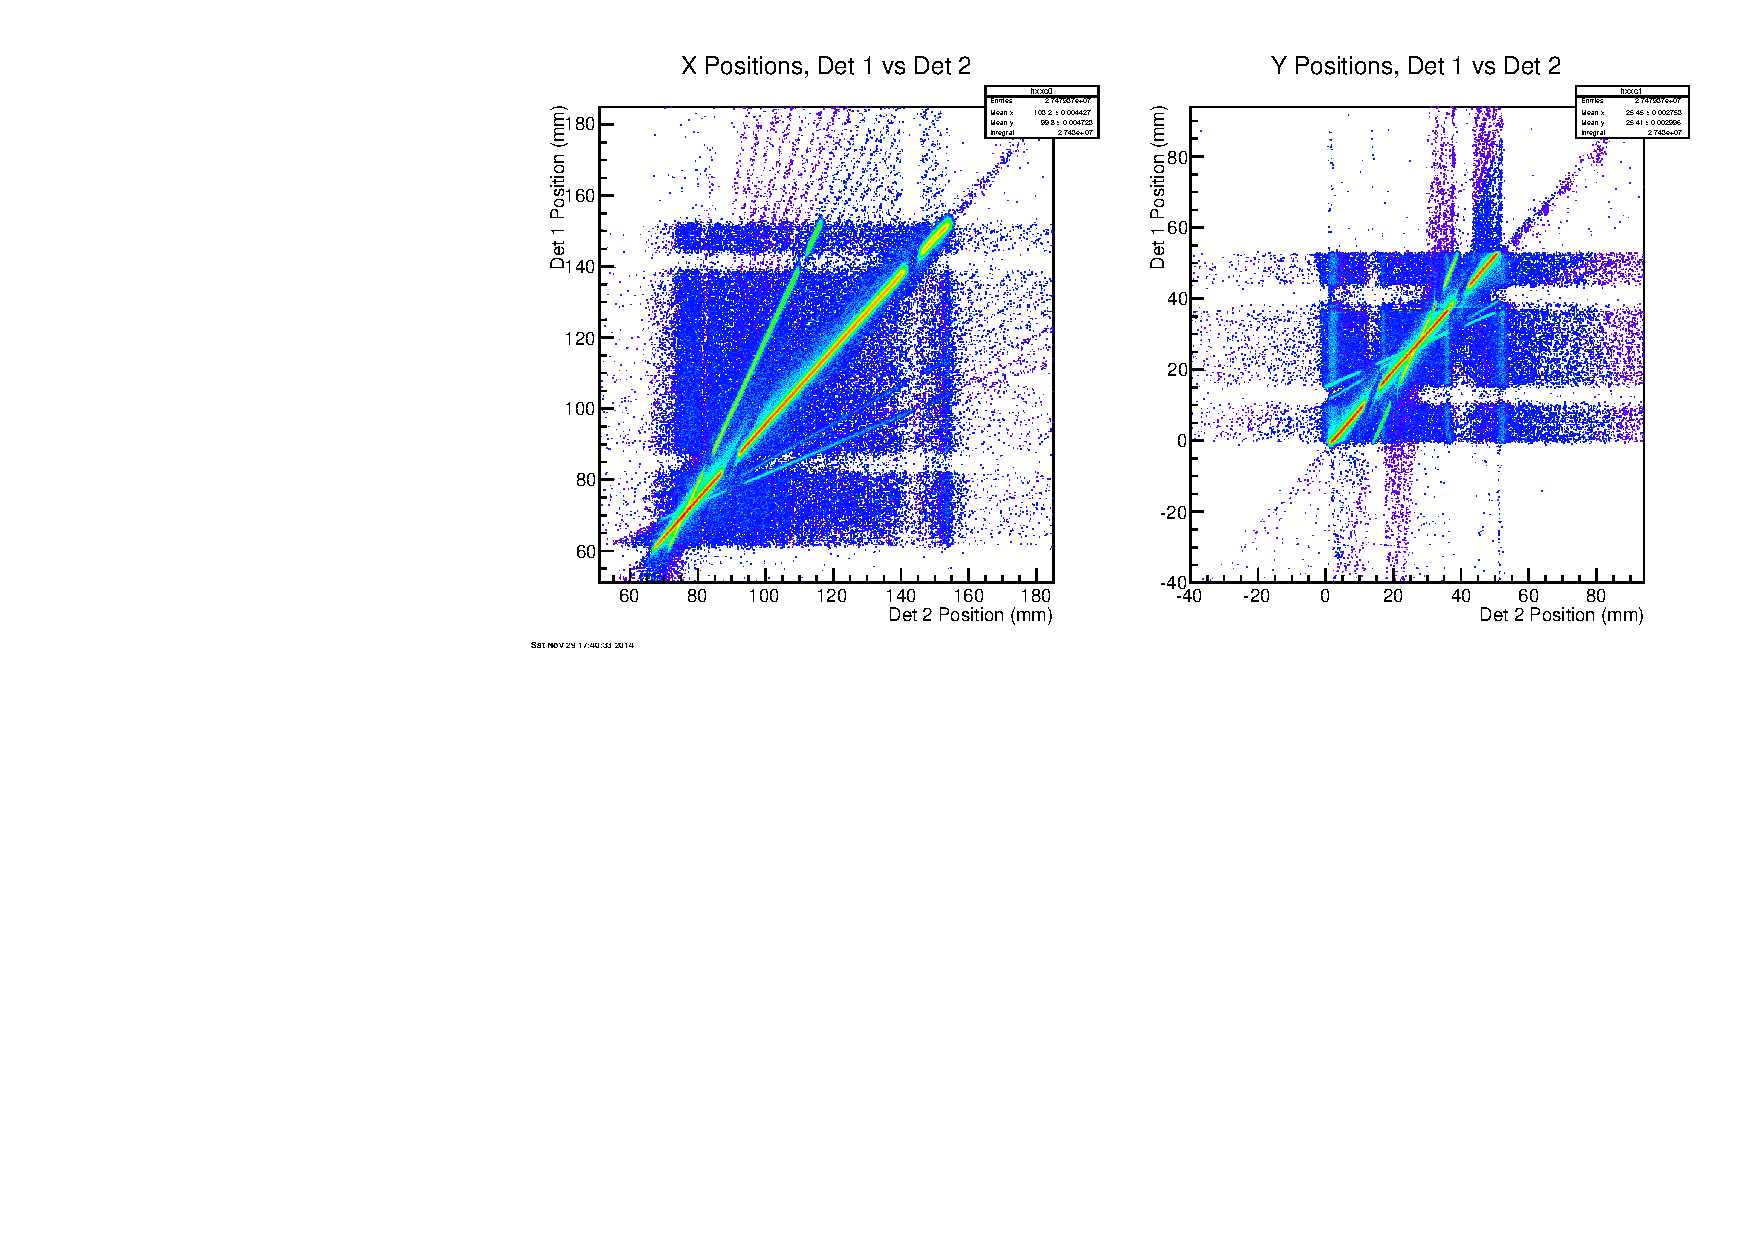
\includegraphics[width=\textwidth, height=0.33\textheight, keepaspectratio]{run_430_hxxc_2} \\
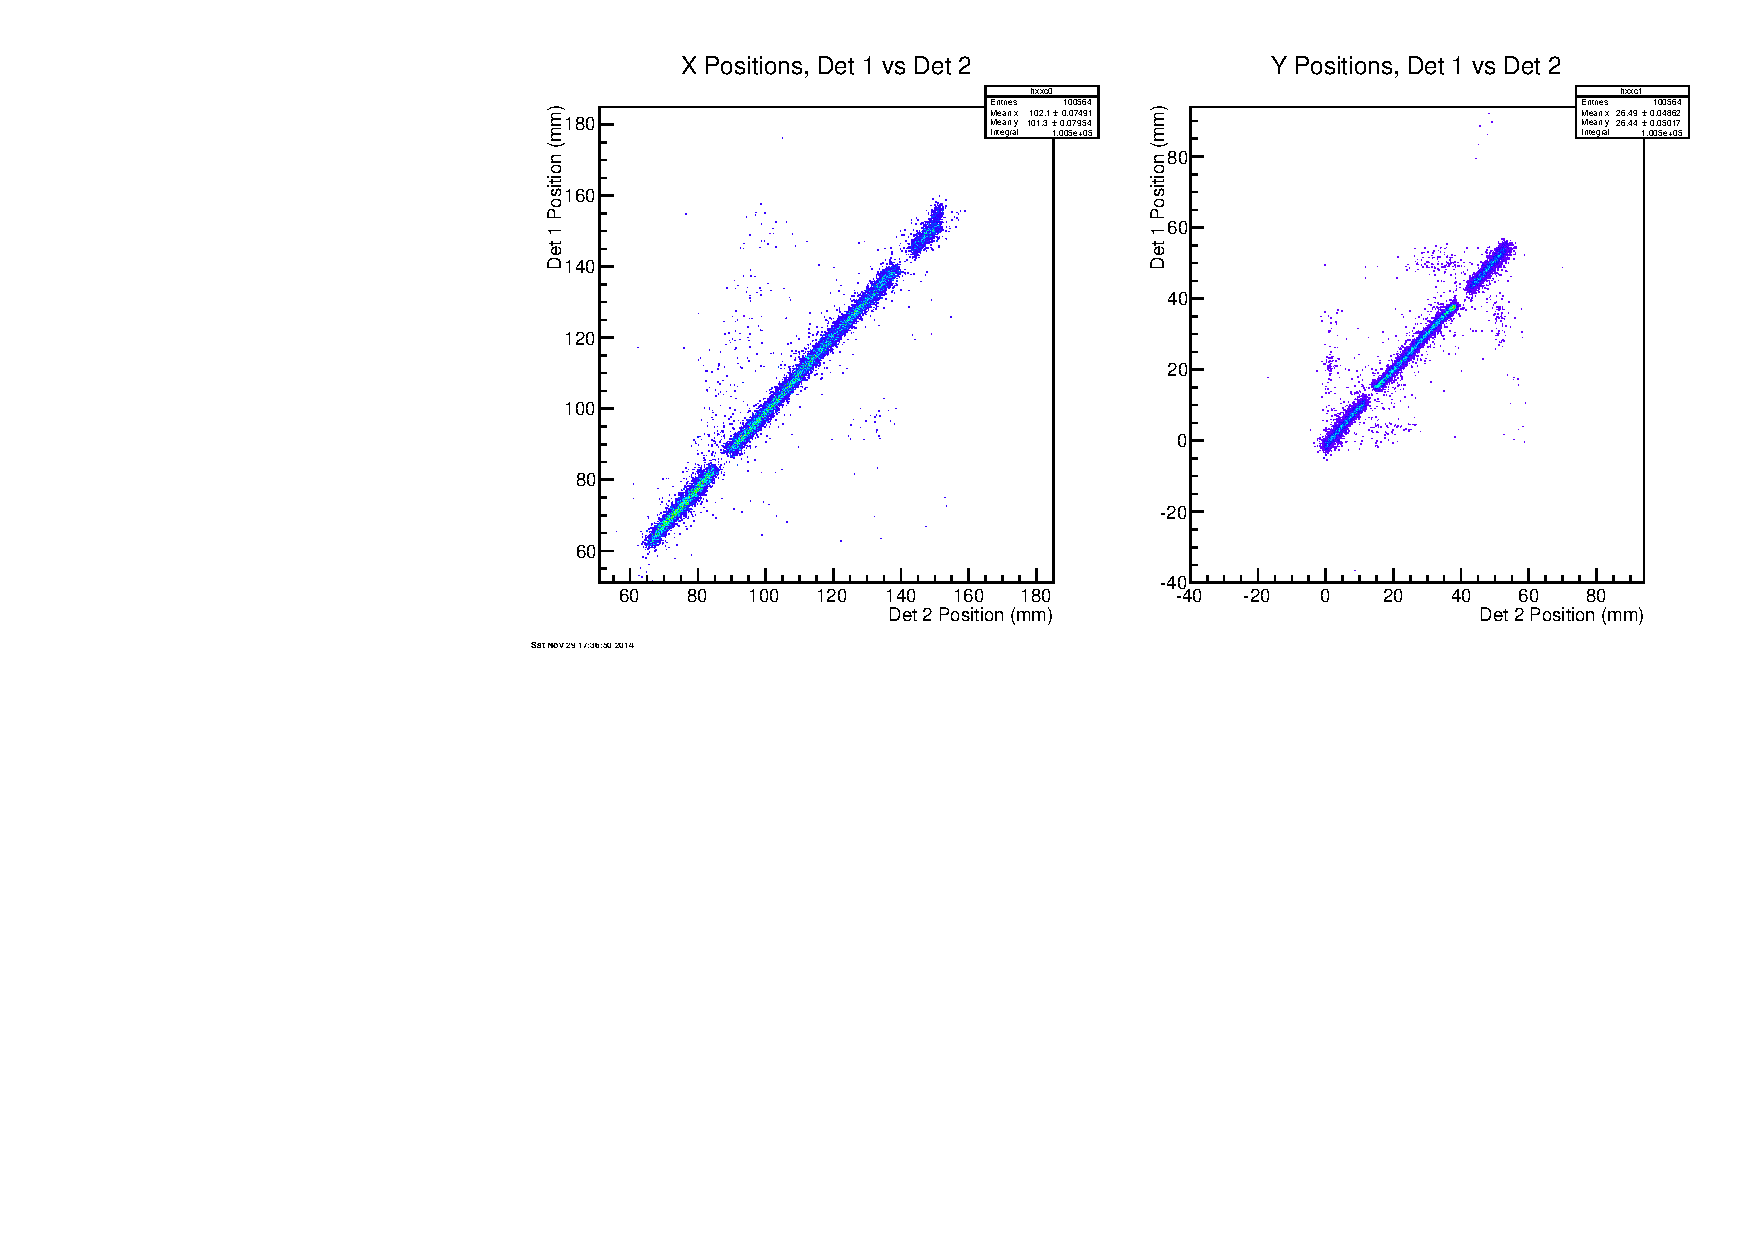
\includegraphics[width=\textwidth, height=0.33\textheight, keepaspectratio]{run_480_hxxc_2} 
\caption{Example  spectra for Run 430 (left) and Run 480 (right). }
\label{hxxc}
\end{figure}

The appearance of unphysical trajectories and random background are consistent with abnormal conditions such as sparking or triggering in the noise. Any of the data runs showing such pathological
Excluding all runs with unphysical behavior that are not otherwise excluded leaves 29 data runs for final analysis. 
\subsubsection{Summary}
The two most useful histograms for selecting data are the anode-time vs. cathode-sum plots (see Fig.~\ref{htsum} and the position correlation plots (see Fig.~\ref{hxxc}). Given an external time reference, the first example will still be useful in the final, single-detector setup.)
\subsection{Settings}
\label{settings_sec}
The detector and beam settings for the 29 data runs that were not excluded are shown in Table~\ref{run_list}. The summary of the 14 different combinations of detector and beam settings is shown in Table~\ref{settings}.
\begin{table}[ht!]
\centering
\begin{tabular}{crc..rccccr}
\hline
\multicolumn{2}{c}{Run} & \multicolumn{2}{c}{ADC} & \multicolumn{2}{c}{Beam} & & \multicolumn{3}{c}{Voltage}\\ \cline{1-2} \cline{5-6} \cline{8-10}
No. & Duration & On & \multicolumn{1}{c}{Sample} & \multicolumn{1}{c}{Current} & Atten. & $P$ & $V_\textrm{c}$ & $V_\textrm{a}$ & $\Delta V$ & Coinc.\\
\hline \hline
%438 & 598 & 0 & 1 & 5.62 & 10 & 3 & -74 & 411 & 485 & 32,159\\
%439 & 1154 & 1 & 5 & 5.62 & 10 & 3 & -74 & 411 & 485 & 16,836\\
%440 & 762 & 1 & 2.5 & 5.69 & 10 & 3 & -74 & 411 & 485 & 15,420\\
%444 & 397 & 1 & 1 & 5.69 & 10 & 4 & -80 & 430 & 510 & 24,941\\
%445 & 1,086 & 1 & 1 & 5.80 & 10 & 4 & -80 & 430 & 510 & 19,733\\
%446 & 538 & 1 & 1 & 5.89 & 10 & 4 & -80 & 430 & 510 & 38,811\\
%447 & 315 & 1 & 2.5 & 5.92 & 10 & 4 & -80 & 430 & 510 & 4,916\\
%449 & 294 & 0 & 5 & 5.99 & 10 & 6 & -90 & 470 & 560 & 8,095\\
%450 & 274 & 1 & 5 & 5.95 & 10 & 6 & -90 & 470 & 560 & 39,730\\
%451 & 244 & 1 & 5 & 5.86 & 10 & 6 & -90 & 480 & 570 & 28,987\\
%452 & 242 & 1 & 2.5 & 5.82 & 10 & 6 & -90 & 480 & 570 & 27,590\\
%454 & 273 & 0 & 1 & 5.75 & 10 & 6 & -90 & 450 & 540 & 38,737\\
%455 & 266 & 1 & 5 & 5.74 & 10 & 6 & -90 & 450 & 540 & 35,818\\
%456 & 690 & 1 & 2.5 & 5.75 & 10 & 6 & -90 & 450 & 540 & 25,818\\
%463 & 242 & 0 & 1 & 4.30 & 10 & 2 & -80 & 400 & 480 & 33,211\\
%465 & 321 & 0 & 1 & 0.52 & 10 & 2 & -80 & 390 & 470 & 22,758\\
%467 & 176 & 1 & 1 & 0.54 & 10 & 2 & -80 & 395 & 475 & 22,083\\
%468 & 327 & 1 & 1 & 0.52 & 10 & 2 & -80 & 395 & 475 & 11,334\\
%470 & 307 & 1 & 1 & 5.60 & 10 & 3 & -75 & 410 & 485 & 5,817\\
%471 & 378 & 1 & 1 & 5.66 & 10 & 3 & -75 & 410 & 485 & 40,467\\
%472 & 285 & 1 & 1 & 5.63 & 10 & 3 & -75 & 390 & 465 & 31,042\\
%473 & 361 & 1 & 1 & 5.59 & 10 & 3 & -75 & 375 & 450 & 20,511\\
%474 & 318 & 1 & 1 & 5.50 & 10 & 4 & -80 & 430 & 510 & 8,141\\
%475 & 429 & 1 & 1 & 5.55 & 10 & 4 & -80 & 430 & 510 & 12,470\\
%476 & 392 & 1 & 1 & 0.51 & 120 & 4 & -80 & 430 & 510 & 29,756\\
%477 & 315 & 1 & 1 & 34.00 & 1 & 4 & -80 & 410 & 490 & 2,679\\
%478 & 72 & 1 & 1 & 0.65 & 120 & 4 & -80 & 445 & 525 & 29,251\\
%479 & 595 & 1 & 1 & 0.65 & 120 & 4 & -80 & 445 & 525 & 2,073\\
%480 & 805 & 1 & 1 & 0.64 & 120 & 3 & -80 & 435 & 515 & 28,465\\
438 & 598 & 1 & 5 & 5.62 & 10 & 3 & -74 & 411 & 485 & 32,159\\
439 & 1154 & 1 & 2.5 & 5.62 & 10 & 3 & -74 & 411 & 485 & 16,836\\
440 & 762 & 1 & 1 & 5.69 & 10 & 3 & -74 & 411 & 485 & 15,420\\
444 & 397 & 1 & 1 & 5.69 & 10 & 4 & -80 & 430 & 510 & 24,941\\
445 & 1086 & 1 & 1 & 5.80 & 10 & 4 & -80 & 430 & 510 & 19,733\\
446 & 538 & 1 & 2.5 & 5.89 & 10 & 4 & -80 & 430 & 510 & 38,811\\
447 & 315 & 1 & 5 & 5.92 & 10 & 4 & -80 & 430 & 510 & 4,916\\
449 & 294 & 1 & 5 & 5.99 & 10 & 6 & -90 & 470 & 560 & 8,095\\
450 & 274 & 1 & 5 & 5.95 & 10 & 6 & -90 & 470 & 560 & 39,730\\
451 & 244 & 1 & 2.5 & 5.86 & 10 & 6 & -90 & 480 & 570 & 28,987\\
452 & 242 & 1 & 1 & 5.82 & 10 & 6 & -90 & 480 & 570 & 27,590\\
454 & 273 & 1 & 5 & 5.75 & 10 & 6 & -90 & 450 & 540 & 38,737\\
455 & 266 & 1 & 2.5 & 5.74 & 10 & 6 & -90 & 450 & 540 & 35,818\\
456 & 690 & 1 & 1 & 5.75 & 10 & 6 & -90 & 450 & 540 & 25,818\\ \hline
463 & 242 & 1 & 1 & 4.30 & 10 & 2 & -80 & 400 & 480 & 33,211\\
465 & 321 & 1 & 1 & 0.52 & 10 & 2 & -80 & 390 & 470 & 22,758\\
467 & 176 & 1 & 1 & 0.54 & 10 & 2 & -80 & 395 & 475 & 22,083\\
468 & 327 & 1 & 1 & 0.52 & 10 & 2 & -80 & 395 & 475 & 11,334\\
470 & 307 & 1 & 1 & 5.60 & 10 & 3 & -75 & 410 & 485 & 5,817\\
471 & 378 & 1 & 1 & 5.66 & 10 & 3 & -75 & 410 & 485 & 40,467\\
472 & 285 & 1 & 1 & 5.63 & 10 & 3 & -75 & 390 & 465 & 31,042\\
473 & 361 & 1 & 1 & 5.59 & 10 & 3 & -75 & 375 & 450 & 20,511\\
474 & 318 & 1 & 1 & 5.50 & 10 & 4 & -80 & 430 & 510 & 8,141\\
475 & 429 & 1 & 1 & 5.55 & 10 & 4 & -80 & 430 & 510 & 12,470\\
476 & 392 & 1 & 1 & 0.51 & 120 & 4 & -80 & 430 & 510 & 29,756\\
477 & 315 & 1 & 1 & 34.00 & 1 & 4 & -80 & 410 & 490 & 2,679\\
478 & 72 & 1 & 1 & 0.65 & 120 & 4 & -80 & 445 & 525 & 29,251\\
479 & 595 & 1 & 1 & 0.65 & 120 & 4 & -80 & 445 & 525 & 2,073\\
480 & 805 & 1 & 1 & 0.64 & 120 & 3 & -80 & 435 & 515 & 28,465\\
\hline
\end{tabular}
\caption{Detector, acquisition, and beam settings from April 2014 for the 29 runs which are not excluded. Given are the run number and the run duration (in seconds). The settings for digitizer, here referred to as the ADC, are given: the enable state and the sample rate (in GS/s). The nominal beam current is given (in enA) and the associated setting of the IOS attenuator is given. Note that for a number of the 2\,Torr runs, the beam current fell off by a factor of $10\times$. The detector settings are given next: pressure (in Torr) and voltage (in V). Finally the number of anode coincidences is given. The horizontal line indicates a new day of testing.}
\label{run_list}
\end{table}

\begin{table}[ht!]
\centering
\begin{tabular}{crc..rccccr}
\hline
\multicolumn{2}{c}{Run} & \multicolumn{2}{c}{ADC} & \multicolumn{2}{c}{Beam} & & \multicolumn{3}{c}{Voltage}\\ \cline{1-2} \cline{5-6} \cline{8-10}
No. & Duration & On & \multicolumn{1}{c}{Sample} & \multicolumn{1}{c}{Current} & Atten. & $P$ & $V_\textrm{c}$ & $V_\textrm{a}$ & $\Delta V$ & Coinc.\\
\hline \hline
%584 & 633 & 0 & 0 & 9.00 &  & 3 & -75 & 410.5 & 485.5 & 0\\
%586 & 294 & 0 & 0 & 8.50 &  & 3 & -75 & 411 & 486 & 0\\ \hline
%587 & 1813 & 0 & 0 & 13.00 &  & 3 & -75 & 410 & 485 & 0\\
%588 & 1221 & 1 & 1 & 12.89 &  & 3 & -75 & 410 & 485 & 0\\
%589 & 2113 & 0 & 0 & 13.00 &  & 3 & -75 & 410 & 485 & 0\\
%590 & 500 & 0 & 0 & 1.20 &  & 3 & -75 & 410 & 485 & 0\\
%592 & 425 & 0 & 0 & 12.95 &  & 3 & -75 & 410 & 485 & 0\\
%593 & 1143 & 0 & 0 & 12.89 &  & 3 & -79 & 410.5 & 489.5 & 0\\
%594 & 1214 & 0 & 0 & 12.71 &  & 2 & -78 & 397 & 475 & 0\\
%595 & 620 & 1 & 1 & 12.65 &  & 2 & -78 & 397 & 475 & 0\\
%596 & 126 & 0 & 0 & 12.60 &  & 2 & -78 & 397 & 475 & 0\\
%597 & 199 & 1 & 2.5 & 12.24 &  & 2 & -78 & 397 & 475 & 0\\
%598 & 152 & 1 & 5 & 12.48 &  & 2 & -78 & 397 & 475 & 0\\
%599 & 103 & 1 & 1 & 12.60 &  & 2 & -78 & 397 & 475 & 0\\
%600 & 153 & 0 & 0 & 12.60 &  & 2 & -78 & 397 & 475 & 0\\
%602 & 1677 & 0 & 0 & 12.13 &  & 2 & -78 & 397 & 475 & 0\\ \hline
%603 & 2247 & 0 & 0 & 20.00 &  & 4 & -82 & 429 & 511 & 0\\
%604 & 345 & 1 & 1 & 20.55 &  & 4 & -82 & 429 & 511 & 0\\
%606 & 1013 & 0 & 0 & 22.42 &  & 4 & -82 & 429 & 511 & 0\\
%607 & 402 & 1 & 1 & 22.42 &  & 4 & -82 & 429 & 511 & 0\\
%608 & 517 & 0 & 0 & 370.00 &  & 4 & -82 & 429 & 511 & 0\\
%609 & 318 & 1 & 1 & 387.34 &  & 4 & -82 & 429 & 511 & 0\\
%610 & 1203 & 1 & 1 & 1.89 &  & 4 & -82 & 429 & 511 & 0\\
%611 & 821 & 1 & 1 & 1.72 &  & 4 & -82 & 429 & 511 & 0\\
584 & 633 & 0 & 0 & 9.00 & 1 & 3 & -75 & 410.5 & 485.5 & 323,593\\
586 & 294 & 0 & 0 & 8.50 & 1 & 3 & -75 & 411 & 486 & 127,047\\ \hline
587 & 1813 & 0 & 0 & 13.00 & 2 & 3 & -75 & 410 & 485 & 1,171,411\\
588 & 1221 & 1 & 1 & 12.89 & 2 & 3 & -75 & 410 & 485 & 9,705\\
589 & 2113 & 0 & 0 & 13.00 & 2 & 3 & -75 & 410 & 485 & 1,381,064\\
590 & 500 & 0 & 0 & 1.20 & 10 & 3 & -75 & 410 & 485 & 28,330\\
592 & 425 & 0 & 0 & 12.95 & 2 & 3 & -75 & 410 & 485 & 273,850\\
593 & 1143 & 0 & 0 & 12.89 & 2 & 3 & -79 & 410.5 & 489.5 & 737,678\\
594 & 1214 & 0 & 0 & 12.71 & 2 & 2 & -78 & 397 & 475 & 779,734\\
595 & 620 & 1 & 1 & 12.65 & 2 & 2 & -78 & 397 & 475 & 10,466\\
596 & 126 & 0 & 0 & 12.60 & 2 & 2 & -78 & 397 & 475 & 79,535\\
597 & 199 & 1 & 2.5 & 12.24 & 2 & 2 & -78 & 397 & 475 & 970\\
598 & 152 & 1 & 5 & 12.48 & 2 & 2 & -78 & 397 & 475 & 22,823\\
599 & 103 & 1 & 1 & 12.60 & 2 & 2 & -78 & 397 & 475 & 1,698\\
600 & 153 & 0 & 0 & 12.60 & 2 & 2 & -78 & 397 & 475 & 94,607\\
%602 & 1677 & 0 & 0 & 12.13 & 2 & 2 & -78 & 397 & 475 & 136,172\\
 \hline
603 & 2247 & 0 & 0 & 20.00 & 3 & 4 & -82 & 429 & 511 & 2,148,241\\
604 & 345 & 1 & 1 & 20.55 & 3 & 4 & -82 & 429 & 511 & 15,532\\
606 & 1013 & 0 & 0 & 22.42 & 3 & 4 & -82 & 429 & 511 & 1,011,153\\
607 & 402 & 1 & 1 & 22.42 & 3 & 4 & -82 & 429 & 511 & 2,746\\
608 & 517 & 0 & 0 & 370.00 & 0.1 & 4 & -82 & 429 & 511 & 3,404,786\\
609 & 318 & 1 & 1 & 387.34 & 0.1 & 4 & -82 & 429 & 511 & 8,507\\
610 & 1203 & 1 & 1 & 1.89 & 10 & 4 & -82 & 429 & 511 & 2,904\\
611 & 821 & 1 & 1 & 1.72 & 10 & 4 & -82 & 429 & 511 & 23,338\\


\hline
\end{tabular}
\caption{Detector, acquisition, and beam settings for the 24 data runs from the April 2015 in-beam tests. Given are the run number and the run duration (in seconds). The settings for digitizer, here referred to as the ADC, are given: the enable state and the sample rate (in GS/s). The nominal beam current is given (in enA) and the associated setting of the IOS attenuator is given.
% Note that for a number of the 2\,Torr runs, the beam current fell off by a factor of $10\times$.
 The detector settings are given next: pressure (in Torr) and voltage (in V). Finally the number of anode coincidences is given. Data from each of the three days are separated by horizontal lines.}
\label{run_list_2}
\end{table}

\begin{table}[ht!]
\centering
\begin{tabular}{cccc.rrr}
\hline
& \multicolumn{3}{c}{Voltage} & \multicolumn{2}{c}{Beam}\\ \cline{2-4} 
$P$& $V_\textrm{c}$ & $V_\textrm{a}$ & $\Delta V$ & \multicolumn{1}{c}{Current} & Atten. & \multicolumn{1}{c}{Duration} & \multicolumn{1}{c}{Coinc.}\\
\hline \hline
2 & -80 & 390 & 470 & 0.52 & 10 & 321 & 22,758\\
2 & -80 & 395 & 475 & 0.53 & 10 & 503 & 33,417\\
2 & -80 & 400 & 480 & 4.30 & 10 & 242 & 33,211\\ \hline
3 & -75 & 375 & 450 & 5.59 & 10 & 361 & 20,511\\
3 & -75 & 390 & 465 & 5.63 & 10 & 285 & 31,042\\
3 & -74 & 411 & 485 & 5.64 & 10 & 3,199 & 110,699\\
3 & -80 & 435 & 515 & 0.64 & 120 & 805 & 28,465\\ \hline
4 & -80 & 410 & 490 & 34.00 & 1 & 315 & 2,679\\
4 & -80 & 430 & 510 & 5.73 & 10 & 3,083 & 109,012\\
4 & -80 & 430 & 510 & 0.51 & 120 & 392 & 29,756\\
4 & -80 & 445 & 525 & 0.65 & 120 & 667 & 31,324\\ \hline
6 & -90 & 450 & 540 & 5.75 & 10 & 1,229 & 100,373\\
6 & -90 & 470 & 560 & 5.97 & 10 & 568 & 47,825\\
6 & -90 & 480 & 570 & 5.84 & 10 & 486 & 56,577\\
\hline
\end{tabular}
\caption{Summary of the different detector and beam settings used for the 2014 test. For each detector setting, the average beam current is given (in enA) and the associated IOS attenuator setting. Similarly, the total duration of the runs (in seconds) and the total anode coincidences are given.}
\label{settings}
\end{table}
\subsubsection{Detector}
In the 2014 tests, four different pressures were tested. At each pressure, the voltage was varied in order %The goal of the experiment was 
to determine the maximum stable operating voltage. The maximum stable operating voltage was determined by the highest voltage the detector was able to maintain for 5--10\,minutes without sparking. If a spark occurred within that interval, the bias voltage was reduced and the timing procedure was restarted. Such as with the $P=2$\,Torr data shown in Table~\ref{run_list}, depending on the step size used to reduce the voltage, the voltage may then be further increased. For each pressure, at least three different voltages were tested which yielded adequate data. 

Table~\ref{max_V} shows the results of the maximum stable operating pressure tests. For these tests, the IOS attenuator setting remained constant at $10\times$ and the nominal beam current was 5.70\,enA. The relationship between the detector pressure $P$ and the maximum stable voltage difference $\Delta V_\textrm{max}$ is linear and described by the following equation.
\begin{equation}
\Delta V_\textrm{max}=16.86 P%\,\frac{\textrm{V}}{\textrm{torr}}
 +  439.3%\,\textrm{V}
\label{eq:vmax}
\end{equation}
Here the voltage difference $\Delta V_\textrm{max}$ is given in V and the pressure $P$ is given in V/torr. %$\dfrac{\textrm{V}}{\textrm{torr}}$
The average ratio between the maximum stable voltage difference and the maximum stable anode voltage is 83.9\%.
\begin{equation}
V_\textrm{a}=0.839 \Delta V_\textrm{max}
\label{eq:vamax}
\end{equation}
Here both values are given in volts. The calculated maximum stable operating voltages are also %results of these two equations are 
given in Table~\ref{max_V}.

\begin{table}[!ht]
\centering
\begin{tabular}{cccc|ccc}
\hline
& \multicolumn{3}{c|}{Measured}  %\cline{2-4} 
& \multicolumn{3}{c}{Calculated} \\ \cline{2-7} 
$P$& $V_\textrm{c}$ & $V_\textrm{a}$ & $\Delta V$ & $V_\textrm{c}$ & $V_\textrm{a}$ &$\Delta V_\textrm{calc}$ \\
\hline \hline
%2 & -80 & 395 & 475&473.0\\
%3 & -75 & 410 & 485&489.9\\
%4 & -80 & 430 & 510&506.7\\
%6 & -90 & 450 & 540&540.4\\
1.5 & --- &--- & --- & 389.6 & -75.0 & 464.6\\
2.0 & -80 &395 & 475 & 396.6 & -76.4 & 473.0\\
2.5 & --- &--- & --- & 403.7 & -77.7 & 481.4\\
3.0 & -75 &410 & 485 & 410.8 & -79.1 & 489.9\\
3.5 & --- &--- & --- & 417.9 & -80.4 & 498.3\\
4.0 & -80 &430 & 510 & 424.9 & -81.8 & 506.7\\
4.5 & --- &--- & --- & 432.0 & -83.2 & 515.1\\
5.5 & --- &--- & --- & 446.1 & -85.9 & 532.0\\
6.0 & -90 &450 & 540 & 453.2 & -87.2 & 540.4\\
\hline
\end{tabular}
\caption{Maximum stable voltage settings for each pressure determined from the 2014 tests. The beam current was nominally 5.70\,enA for these tests. Where available, the measured maximum stable voltages are given. The maximum statable voltage $\Delta V_\textrm{calc}$ %is related to the 
is %can be
 calculated for %an arbitrary
 each pressure using by Eq.~\ref{eq:vmax}.  The calculated ratio between $V_\textrm{a}$  and $\Delta V_\textrm{calc}$ is given by Eq.~\ref{eq:vamax}.}
\label{max_V}
\end{table}
\subsubsection{Beam}
A beam rate test was carried out at $P=4$\,Torr. Three different beam attenuator settings were used. As expected, the lower the beam current, the higher the voltage difference the detector was able to support without sparking. In the final moments of the experiment, the detector was tested at $P=3$\,Torr with the low beam current setting. Again, a higher maximum stable voltage was possible. Note that during the $P=2$\,Torr runs, the beam current dropped off by a factor of $10\times$. This was not due to a change in attenuator setting.
\subsubsection{Acquisition}
The digitizer (ADC) was operated at three different sampling frequencies: 1.0, 2.5, and 5.0\,GS/s; corresponding to timing resolutions of 1.00\,ns, 400\,ps, and 200\,ps, respectively. The $P=3$\,Torr data at $\Delta V=485$\,V includes all four possible ADC settings---that is, enabled and disabled, and all three sample rates. \marnote{check!}The various ADC settings had no correlation with the resolution of the TDC data.%\pangram{40}

\subsection{Position Resolution}
The width of the sum of cathode signals gives an upper limit on the position resolution. Assessing the position resolution in this way has the benefit of utilizing a simple and reliable fitting algorithm---that is, a least squares fit of a Gaussian function.

\subsubsection{Relative Width}
The relative widths corresponding to the positions remained effectively constant throughout the variety of detector settings. In the 2014 test, Detector 1 had slightly better resolution than detector 2: on average, the width of X2 was 108\% wider than that of X1; and, on average, the width of Y2 was 106\% wider than X1. In the 2015 test, Detector 2 had slightly better position resolution. 
In both tests, the position resolution was better in the $y$-direction. The average width of the $x$-position peaks was 146\%--177\% that of the average width of the $y$-position peaks. Putting all of the position peak widths in terms of the width of Y1:\\% X1 144\%, Y1 100\%, X2 156\%, Y2 106\%.
\begin{center}
\begin{tabular}{ccc}
 \hline 
Pos.& \multicolumn{2}{c}{Ratio} \\ \cline{2-3} 
&2014 & 2015\\\hline\hline
 X1 & 144\%&161\%\\
 Y1 & 100\%&100\%\\
 X2 & 156\%&155\%\\
 Y2 & 106\%&79\%\\\hline
 

\end{tabular}
\end{center}

\subsubsection{Voltage Dependence}
At each of the pressure settings of $P=2$, 3, and 6\,Torr, three different voltage settings were tested at the same beam current which provided nominal data.
For $P=2$ and 3\,Torr  %each pressure,
the data were fit with a quadratic function to determine 
%In each case, the maximum stable voltage was determined to be the lowest voltage given.
the minimum peak width. % was calculated for each pressure. 
For each quantity a global minimization was performed %found
 with the condition that the quadratic coefficient be positive and the discriminant be negative to ensure that a valid minimum was determined.
Table~\ref{pos_res_fit} shows the results of that calculation.

The variation in peak width with applied voltage for the $P=2$\,Torr data was relatively flat, with only X1 showing a clear 
minimum within the rage of voltages tested. Also, because of the falloff in beam current, the results from the $P=2$\,Torr data may be inconclusive. 
The variation in peak width for $P=3$\,Torr is show in Fig.~\ref{min_fit}. Each of the positions had a minimum within the range of measured voltages.
For $P=2$ and 3\,Torr, the results of the fit are in good agreement with the maximum stable operating voltage shown in Table~\ref{max_V}. This independent agreement suggests that the optimal operating voltage is the same as the maximum stable operating voltage.

For the data at $P=4$, 6\,Torr the maximum stable voltage was %determined to be 
the same as the lowest voltage tested. For $P=4$\,Torr, only one point was available for the $10\times$ attenuator setting. For $P=6$\,Torr, the peak width decreased approaching $\Delta V=540$\,V. However, no data for $\Delta V < 540$\,V was measured, so a representative fit could not be made. For $P=4$ and 6\,Torr, the ``Average'' value given in Table~\ref{pos_res_fit} is the result of Eq.~\ref{eq:vmax}.


\begin{figure}
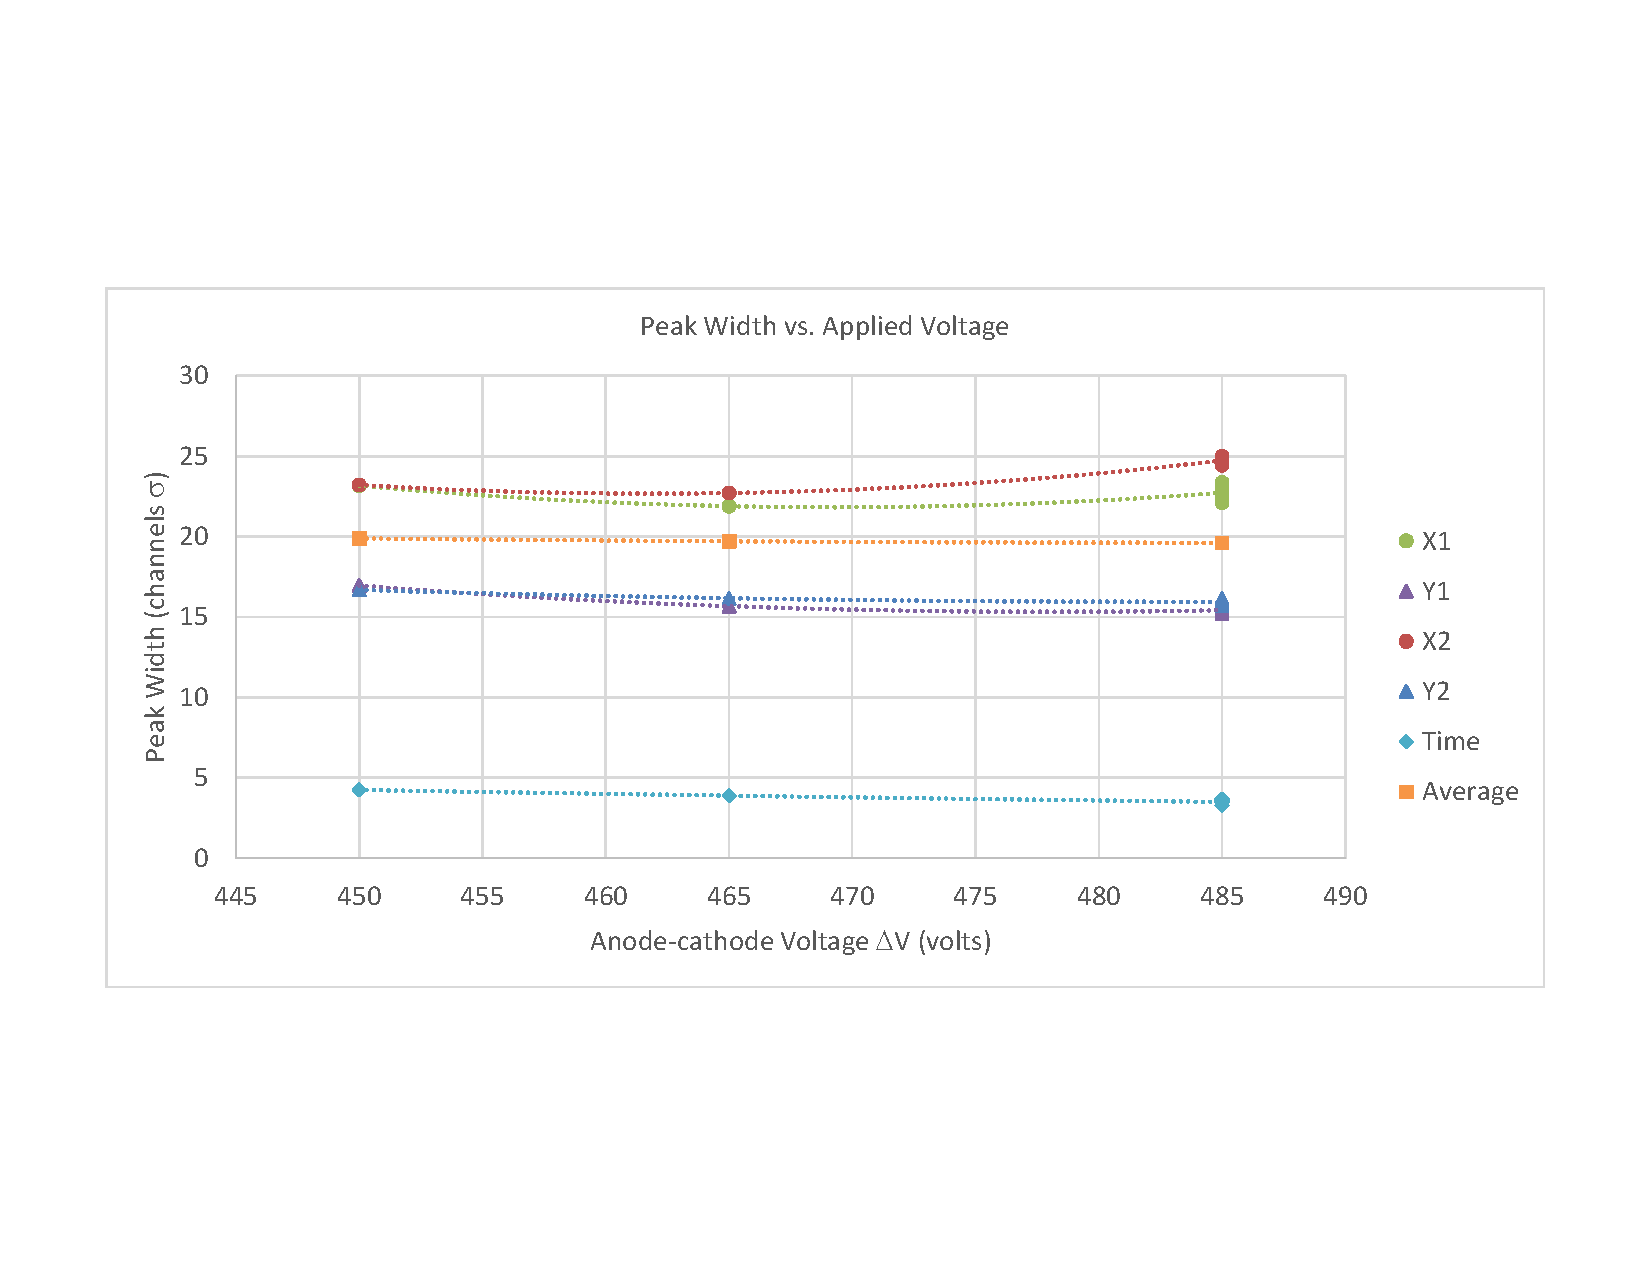
\includegraphics[width=\columnwidth]{PGAC_test_run_list_av_6}%
\caption{Peak width variance with applied voltage %$\Delta V$
 at $P=3$\,Torr. The beam current was nominally 5.70\,enA for all runs. The detector was tested at three different voltages from 450--485V. For each position, the variation of the width of the position peaks was fit with a quadratic function.  The average minimum of these fits was 488.4\,V. The average of the positions is also plotted.}%
\label{min_fit}%
\end{figure}

\begin{table}[ht!]
\centering
\begin{tabular}{cccccccc|c}
\hline
& \multicolumn{2}{c}{Voltage} & \multicolumn{6}{c}{Fit Minima}\\ \cline{4-9}
Pressure & Min & Max & Time & X1 & Y1 & X2 & Y2 & Average\\ \hline \hline
2 & 470 & 480 & 475.0 & 476.0 & 475.3 & 474.0 & 474.9 & 475.0\\
3  & 450 & 485 & --- & 470.4 & 493.5 & 471.5 & 483.4 & 488.4\\
4  & 510 & 510 & --- & --- & --- & --- & --- & 506.7\\
6  & 540 & 570 & --- & --- & --- & --- & --- & 540.4\\
\hline
\end{tabular}
\caption{Calculated optimal voltage for each pressure setting. At each pressure, the maximum and minimum voltage that was tested is given. The beam attenuator setting was the same for all of these runs, with a nominal beam current of 5.70\,enA. Each data set for $P=2$, 3\,Torr was fit with a quadratic function. Where applicable, the minimum of each fit and the average of the minima are given. For $P=4$, 6\,Torr the ``Average'' minimum is given by Eq.~\ref{eq:vmax}. The data for $P=3$\,Torr is shown in Fig.~\ref{min_fit}. }
\label{pos_res_fit}
\end{table}

\subsubsection{Pressure Dependence}
Fig.~\ref{pressure_width} shows the variation of the various peak widths as a function of pressure. For all data sets, the voltage difference is set to the maximum stable operating voltage and the nominal beam current is 5.70\,enA.
 Table~\ref{av_peak_vs_pressure} shows the average peak width for the time and positions at the maximum stable operating voltage at each pressure. Recall the time peak is the difference of the anode signals; and the position peaks are the sum of the cathode signals. Each data set for each position has been fit with a quadratic function.


\begin{figure}
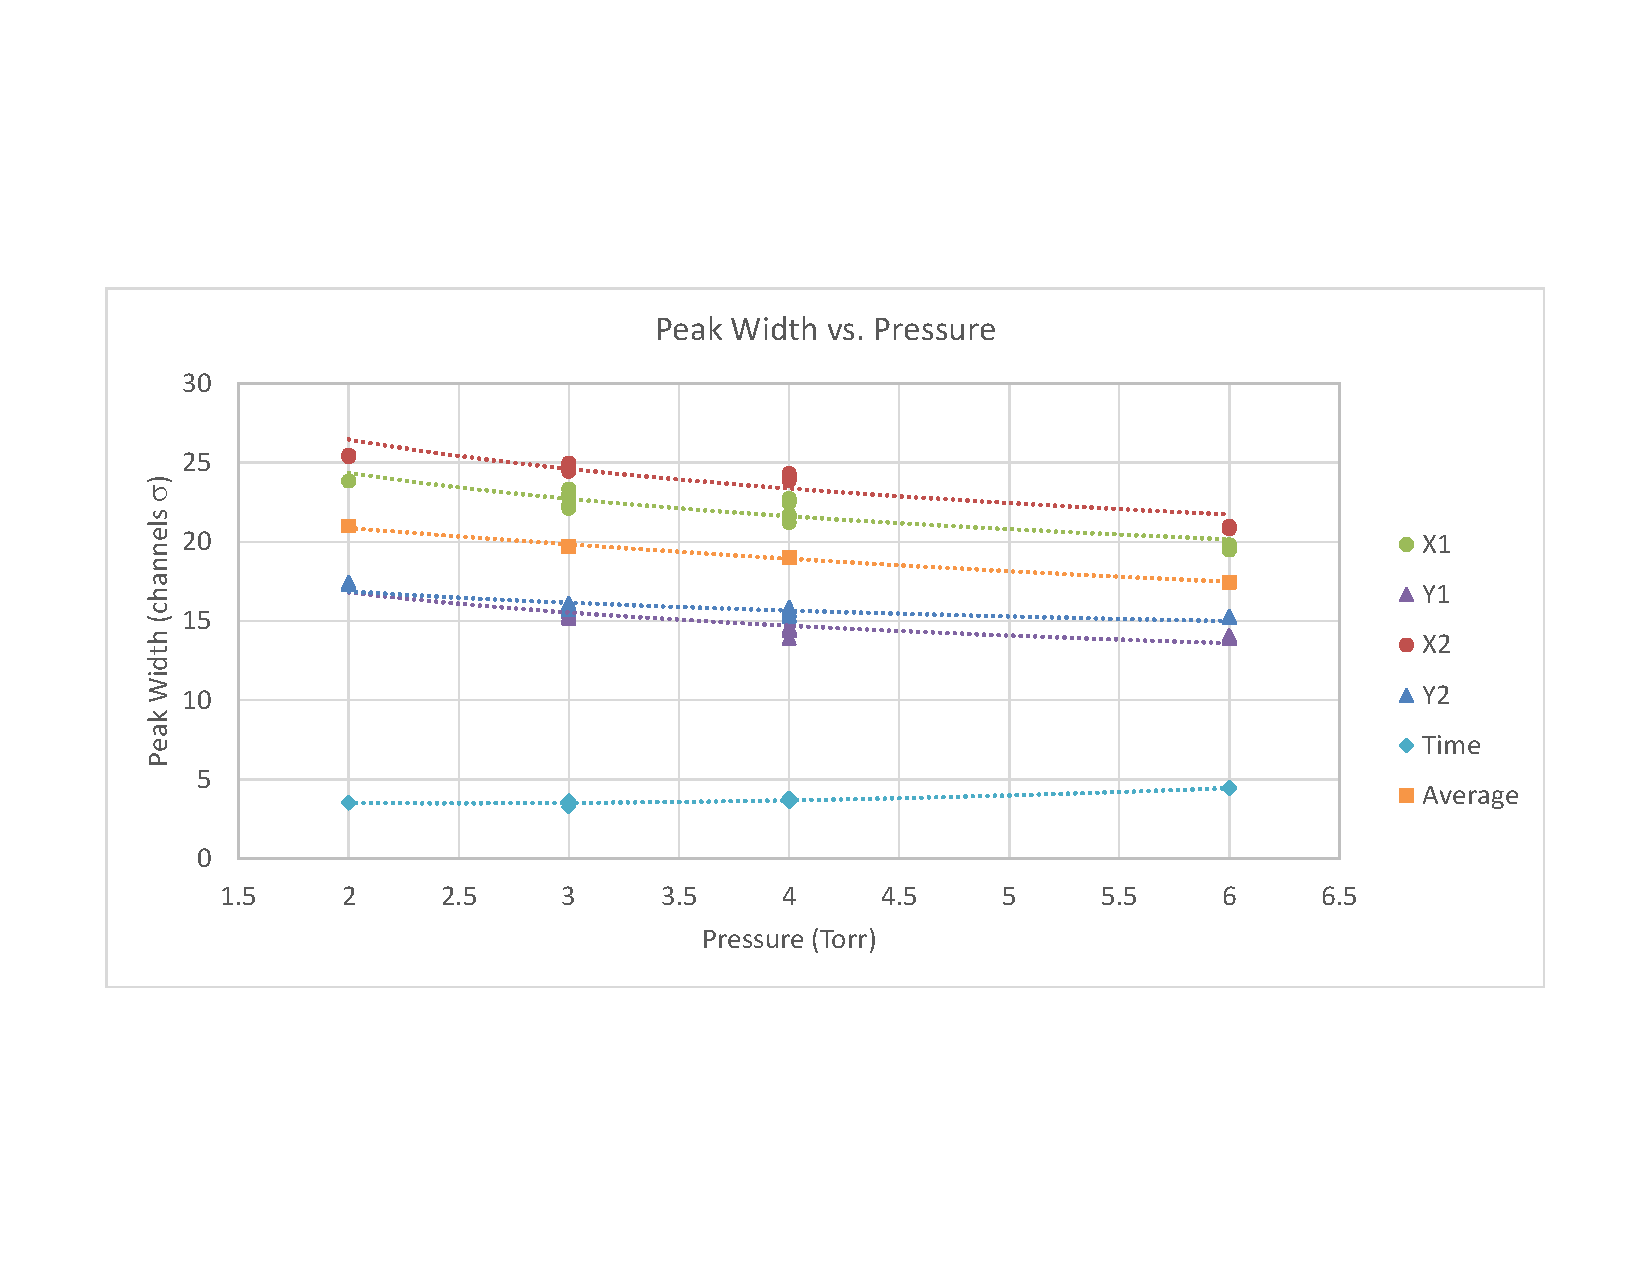
\includegraphics[width=\columnwidth, height=0.33\textheight, keepaspectratio]{PGAC_test_run_list_width_vs_P_6}%
\caption{Peak width variance with pressure. For each pressure setting, the detector is biased to the maximum stable operating voltage. The beam current was nominally 5.70\,enA for all runs. Each data set is fit with a quadratic function. The average of the positions is also plotted. These data are also given in Table~\ref{av_peak_vs_pressure}.}%
\label{pressure_width}%
\end{figure}

\begin{table}
\centering
\begin{tabular}{cccc|...}
\hline
& \multicolumn{3}{c}{Max Voltage} &\multicolumn{3}{c}{Average Peak Width}\\ \cline{2-4} \cline{2-4} \cline{5-7} 
$P$& $V_\textrm{c}$ & $V_\textrm{a}$ & $\Delta V$ &\multicolumn{1}{c}{Time}&\multicolumn{1}{c}{X}&\multicolumn{1}{c}{Y}\\
\hline \hline
2 & -80 & 395 & 475 & 3.54 & 24.64 & 17.39\\
3 & -75 & 410 & 485 & 3.50 & 23.72 & 15.68\\
4 & -80 & 430 & 510 & 3.69 & 23.06 & 14.98\\
6 & -90 & 450 & 540 & 4.46 & 20.27 & 14.64\\
\hline
\end{tabular}
\caption{Average peak width at the maximum stable operating voltage at each pressure. These data are plotted in Fig.~\ref{pressure_width}.}
\label{av_peak_vs_pressure}
\end{table}

\subsubsection{Position Dependence}
The output of the commands \texttt{peakfit()}, \texttt{peakfits()}, or \texttt{peakfity()}, in addition to providing linear position calibration, these commands will also output a plot of the individual peak widths. Given the global fit from which these parameters are generated, this is the most accurate procedure to assess the resolution of the detector. The width of the peaks shown in Fig.~\ref{peakfit} is shown in  Fig.~\ref{pos_width}.

\begin{figure}
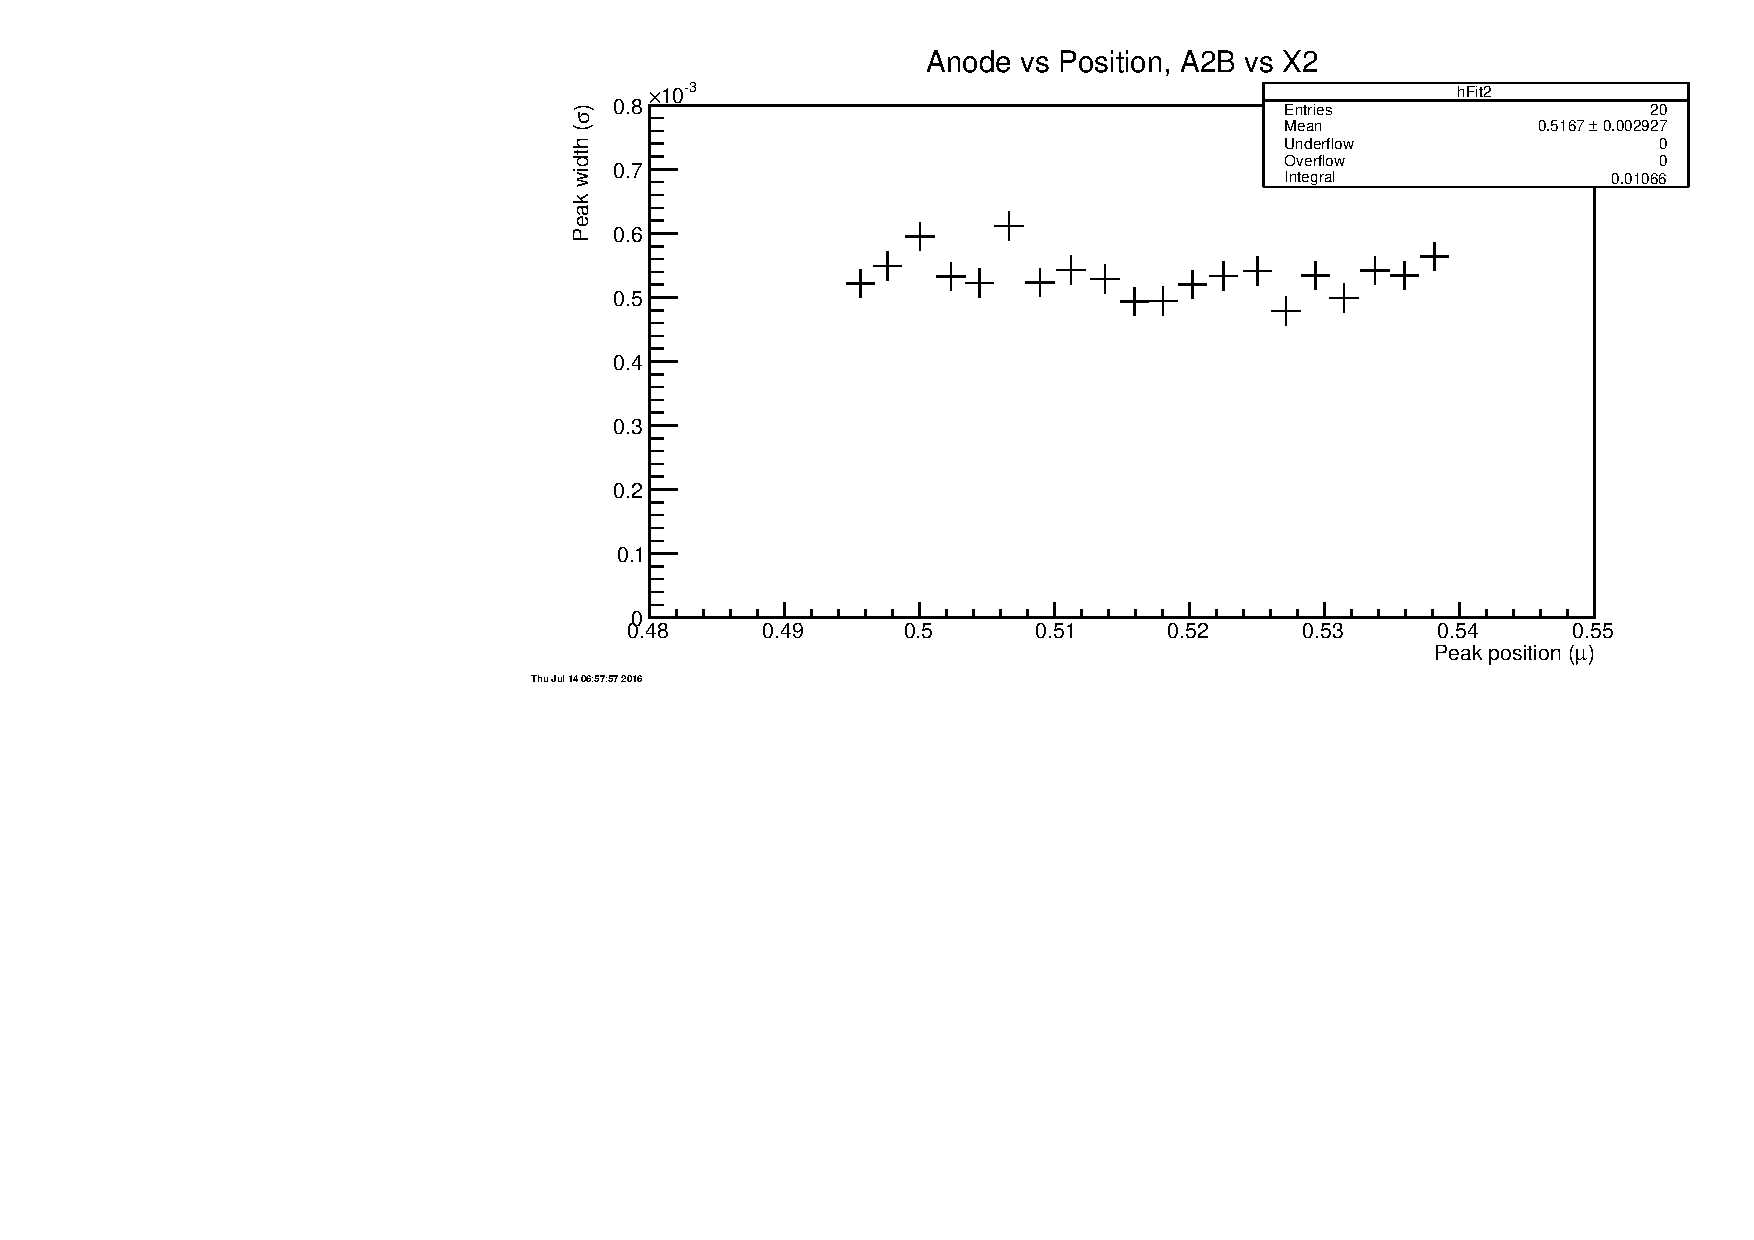
\includegraphics[width=\columnwidth, keepaspectratio]{run_606_width}%
\caption{Measured width of the peaks shown in Fig.~\ref{peakfit}. The widths are given in terms of the Gaussian fit parameter $\sigma$.}%
\label{pos_width}%
\end{figure}

\subsection{Timing Resolution}
The relationship between the anode signals was very sharply defined.  This allowed the anode signals to be gain-matched by applying a linear fit to a two-dimensional plot as shown in Fig.~\ref{lin_fit}.  
Equation~\ref{correlation} gives the relationship between the resolution 
%variance
 of the measured time $\sigma_{t}$ and the individual detector resolutions, $\sigma_{a1}$ and $\sigma_{a2}$.
\begin{equation}
\sigma_t^2=\sigma_{a1}^2+\sigma_{a2}^2-2\sigma_{a1}\sigma_{a2}
\label{correlation}
\end{equation}
Despite the clear correlation between the two anode signals (cf. Fig.~\ref{lin_fit}), the time measured by one anode does not effect the time measured by the other anode.  Therefore, in terms of the covariance of the two time measurements, the anode signals are uncorrelated.  This means that the last term in Eq.~\ref{correlation} is zero.  Assuming that the time resolution of both detectors is the same, Eq.~\ref{correlation} reduces to
\begin{equation}
  \sigma_{a}=\frac{1}{\sqrt{2}}\sigma_{t}.
\end{equation}

Therefore, to determine the timing resolution of an individual detector, the values of the timing resolution of the differences given in Tables~\ref{time_res} and \ref{time_res2} are divided by $\sqrt{2}$.
\paragraph{2014 Tests} 
For example, consider the width of the time difference  between the middle anode segments shown in Fig.~\ref{time_pos}; the width of the $y$-projection of the peak which is 2.23\,channels (sigma).  The TDC has a resolution of 200\,ps/channel.  Therefore the difference between the anode signals is calibrated to time in ns by dividing the channel number by 5.  In this case, the width of the difference corresponds to 446\,ps (sigma).  For an individual detector, this width is equivalent to 315\,ps (sigma) or 743\,ps~FWHM. The widths of the various time peaks is given in Table~\ref{time_res}.

\paragraph{2015 Tests} 
The timing resolution from the 2015 tests is given in Table~\ref{time_res2}.


\begin{figure}%
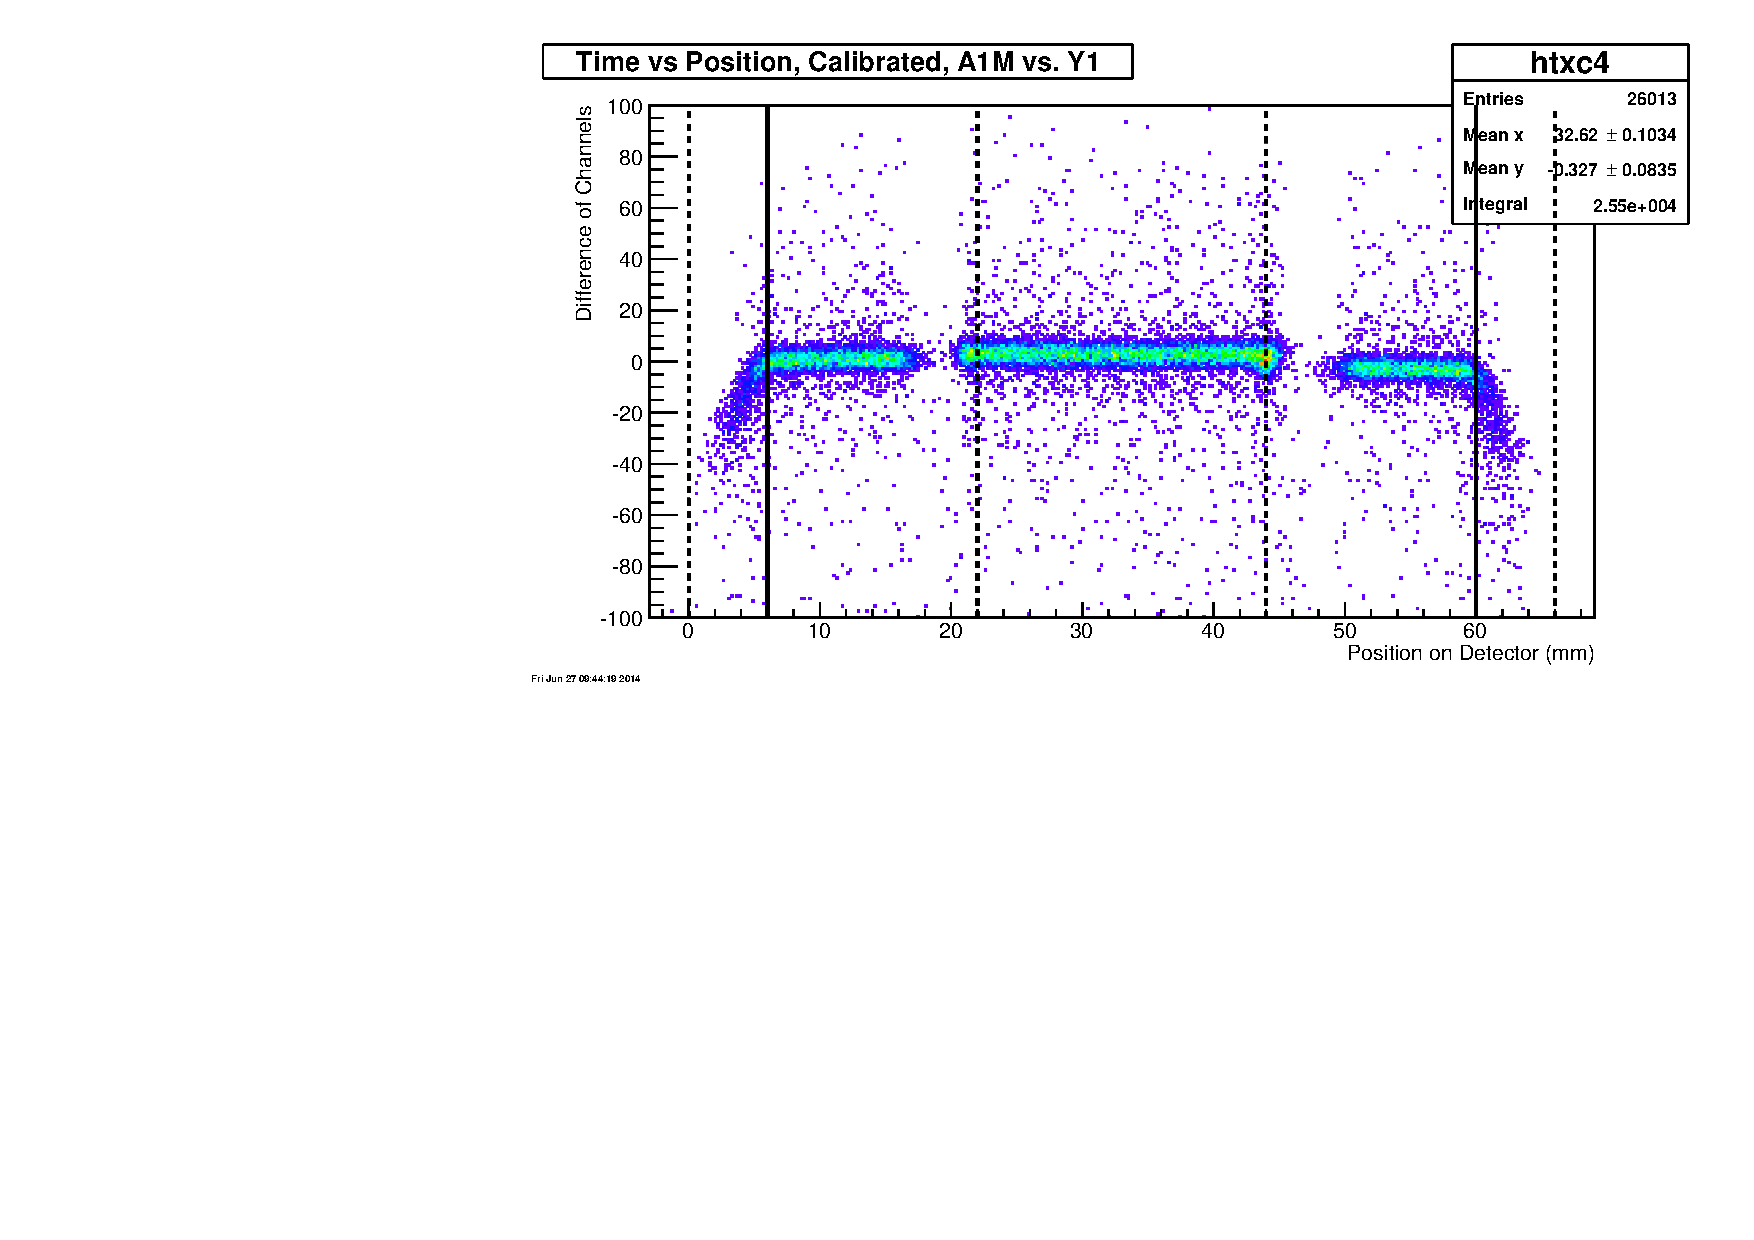
\includegraphics[width=\columnwidth]{run00480_htxc4}%
\caption{Plot of uncalibrated time vs. $y$-position on detector 1.  Solid lines indicate the positions of the Kapton shields.  Dashed lines indicate the edges of the anode segments.}%
\label{time_pos}%
\end{figure}
%\subsubsection{Results}
\begin{table}[ht!]
\centering
\begin{tabular}{-.....}
\hline
&\multicolumn{2}{c}{Pair}&&\multicolumn{2}{c}{Individual}\\ \cline{2-3} \cline{5-6}
\multicolumn{1}{c}{Reference}&\multicolumn{1}{c}{$\sigma$ (ns)}&\multicolumn{1}{c}{FWHM (ns)}&\multicolumn{1}{c}{$\mu$ (ns)}
                             &\multicolumn{1}{c}{$\sigma$ (ns)}&\multicolumn{1}{c}{FWHM (ns)}\\ \hline \hline
\textrm{A2}-\textrm{A1 (all)} & 0.6609 & 1.5563 & 0.0021 & 0.4673 & 1.1005\\
\textrm{A2B}-\textrm{A1B}     & 0.4730 & 1.1139 & -0.1616 & 0.3345 & 0.7877\\
\textrm{A2M}-\textrm{A1M}     & 0.4460 & 1.0502 & 0.2693 & 0.3154 & 0.7426\\
\textrm{A2T}-\textrm{A1T}     & 0.4656 & 1.0964 & -0.9179 & 0.3292 & 0.7753\\
%A2T-A1T (all)  & 0.6378 & 1.5019 & 0.4682\\
%\textrm{A2T}-\textrm{A1T (all)} & 0.6378&1.5019 &0.4682\\
\multicolumn{1}{c}{Average} & 0.4615 & 1.0868 & \multicolumn{1}{c}{---} & 0.3264 & 0.7685 \\
\hline
\end{tabular}
\caption{Timing resolution of the entire detector and the various anode segments. The timing between pairs of anode segments is given, excluding the overlap region near $x=44$\,mm. The equivalent timing resolution of an individual detector is also given (calculated by dividing by $\sqrt{2}$).
%\textit{<These values need to be updated; they are from before the anode signals were fully optimized and are little high.>}
}
\label{time_res}
\end{table}

\begin{table}[ht!]%
\centering
\begin{tabular}{-.....}
\hline
&\multicolumn{2}{c}{Pair}&&\multicolumn{2}{c}{Individual}\\ \cline{2-3} \cline{5-6}
\multicolumn{1}{c}{Reference}&\multicolumn{1}{c}{$\sigma$ (ns)}&\multicolumn{1}{c}{FWHM (ns)}&\multicolumn{1}{c}{$\mu$ (ns)}
                             &\multicolumn{1}{c}{$\sigma$ (ns)}&\multicolumn{1}{c}{FWHM (ns)}\\ \hline \hline
\textrm{A2B}-\textrm{A1B}   & 0.395 & 0.930 & 1.26 &0.279 & 0.658\\ 
\textrm{A2M}-\textrm{A1M}   &0.430 & 1.013 & -1.88 & 0.304 & 0.716\\ 
\textrm{A2T}-\textrm{A1T}   &0.369 & 0.868 & 0.53 & 0.261 & 0.614\\
\multicolumn{1}{c}{Average} & 0.398 & 0.937 &\multicolumn{1}{c}{---} & 0.281 & 0.663\\ \hline
\textrm{A2M}-\textrm{A1B}   & 0.928 & 2.185 & -44.41& 0.656 & 1.545\\ 
\textrm{A2B}-\textrm{A1M}   & 0.919 & 2.163 &-50.38 & 0.650 & 1.530\\ 
\textrm{A2M}-\textrm{A1T}   & 1.107 & 2.606 &-51.36 &0.783 & 1.843\\ 

\hline
\end{tabular}
\caption{Timing resolution of the various anode segments, given for Run 593. The timing between pairs of anode segments is given. The equivalent timing resolution of an individual detector is also given (calculated by dividing by $\sqrt{2}$).
%\textit{<These values need to be updated; they are from before the anode signals were fully optimized and are little high.>}
For reference, those pairs which have sharply-peaked time structure, but do not correspond to ``straight through'' trajectories, are also given.
}
\label{time_res2}
\end{table}

\subsection{Efficiency}
The left panel of Fig.~\ref{ruth} is similar to the final output from the \texttt{peakfit} commands. It shows the calculated area of each of the individual Gaussian fits using the equation
\begin{equation}
  \sigma\sqrt{2\pi} A.
\end{equation}
where $\sigma$ is the width of the fit and $A$ is the amplitude, given by the Gaussian fit parameters \texttt{0} and \texttt{2}, respectively. These values give an approximation of the number counts in the histogram attributable to each peak. The number of counts attributable to each peak would be directly related to the efficiency of the detector at the position of the peak if the detector was uniformly illuminated. However, the detector is not uniformly illuminated. The number of counts at each peak corresponds the Rutherford scattering cross section.

\begin{figure}
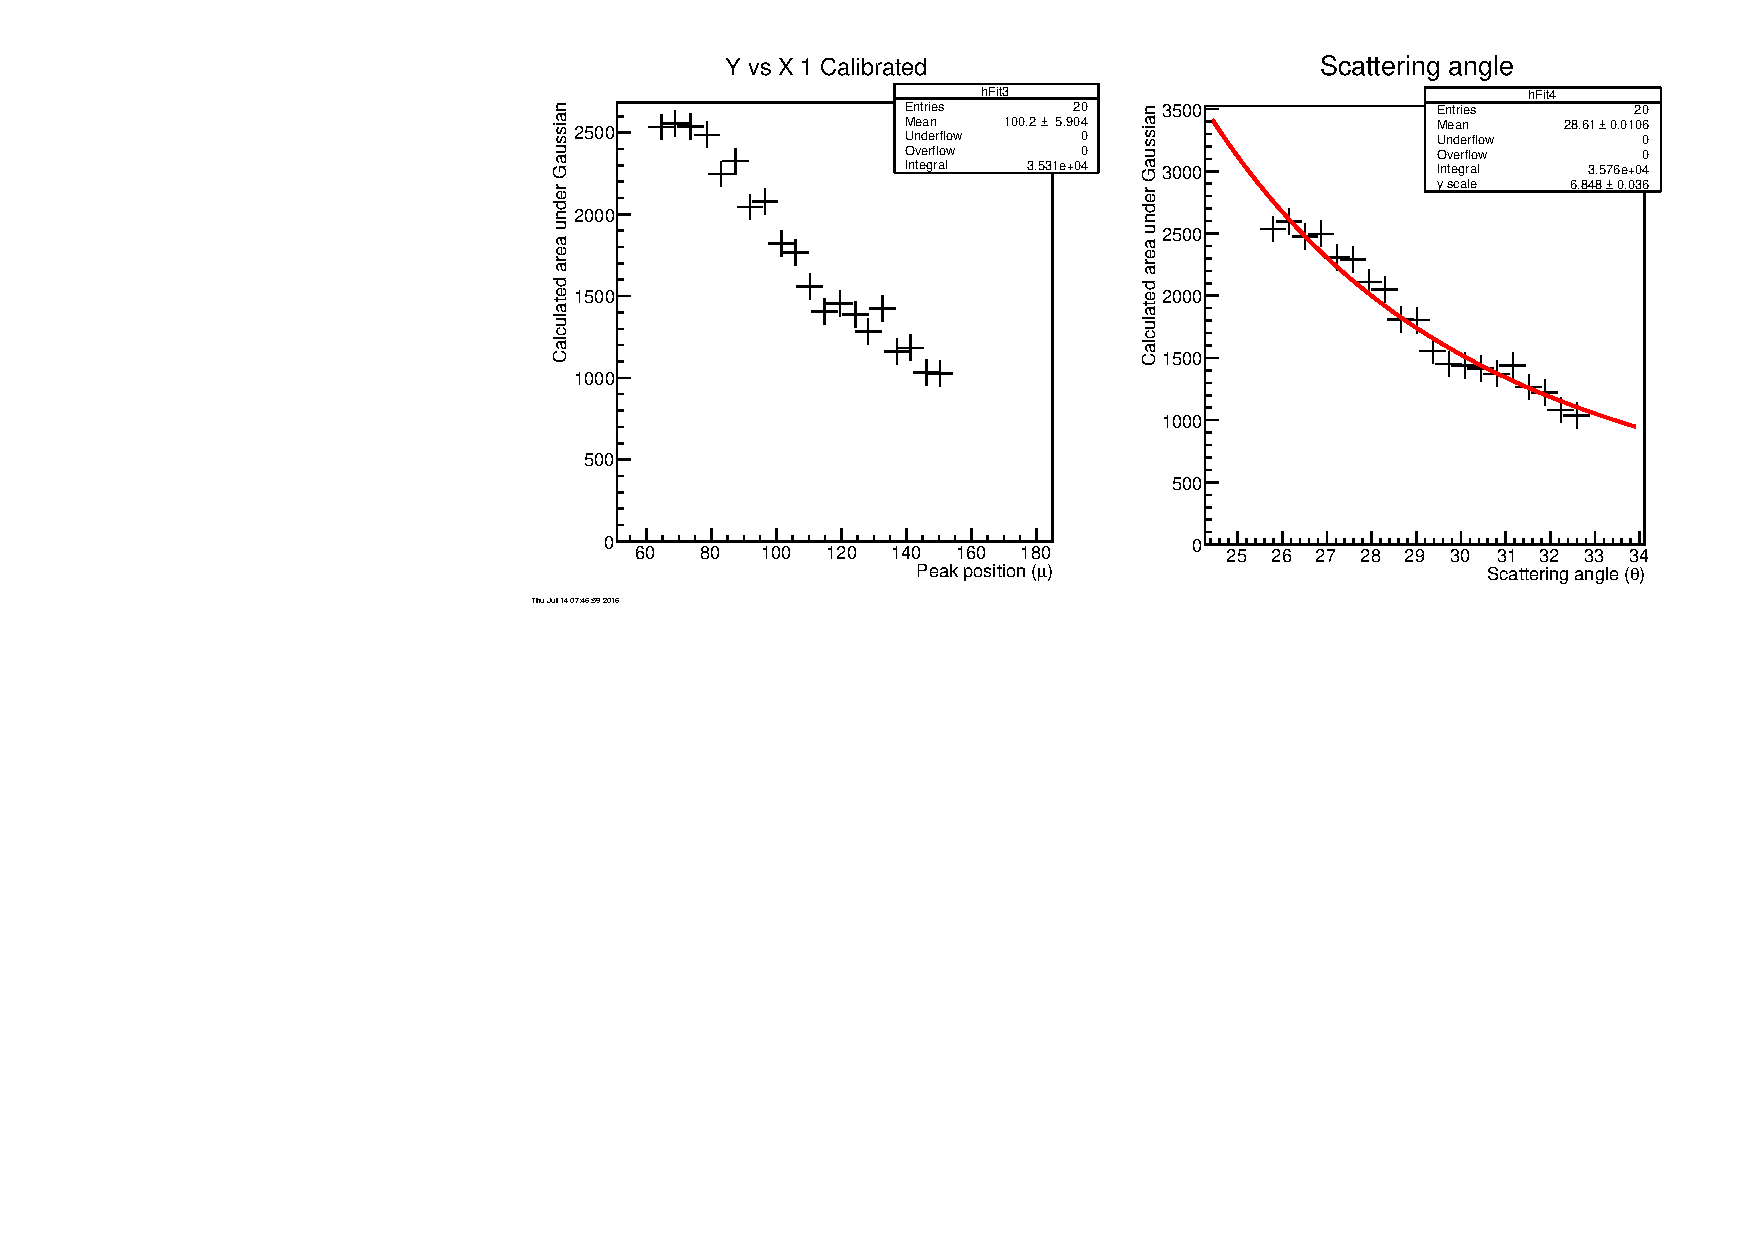
\includegraphics[width=\columnwidth, keepaspectratio]{run_606_ruth}%
\caption{}%
\label{ruth}%
\end{figure}

\begin{quote}
\begin{Verbatim}[firstnumber=0]
readandruth(0,3)
\end{Verbatim}
\end{quote}
The command \texttt{readandruth()} is an extension to the \texttt{peakfit} commands which includes the calculation of the Rutherford scattering cross section. The command takes as input two arguments. First, the detector number---\texttt{0} for detector 1 (downstream) and \texttt{1} for detector 2 (upstream). Right now only detector 1 is fully coded. The command makes a projection of the calibrated 2D position spectra---or ``hit patterns''---named \texttt{hhitc}. The second argument of the command gives the row number to measure, starting from the bottom of the detector. Calibration files are automatically read in so the position of the rows are known. After a particular row is selected, an $x$-projection is made thus giving the position spectrum for one row of peaks on the detector.

The normal peak-fitting routine is then run on the position spectrum. The final output of the peak-fitting routine, shown in the left panel of Fig.~\ref{ruth}, is the calculated area under the curve for each peak, given as a function of the calibrated detector position. The command \texttt{readandruth()} then performs a transformation of coordinates to calculate the scattering angle $\theta$ associated with each detector position. The information about the known height of the row provides the information needed to also calculate the azimuthal angle $\phi$. The plot on the right panel of Fig.~\ref{ruth} is generated, which shows the number of counts attributable to each peak as a function of calculated scattering angle. The distribution is then fit with a $\csc^4 (\theta/2)$ function where the amplitude of the function is a variable parameter. The relationship between the individual peak heights and the fit function may be used to gauge the position-dependence of the detector efficiency.
\section{Appendix}
A number of deprecated calibration procedures are included here for reference.
\subsection{Gaini-matching}
For position signals, one test of the effectiveness of the gain-matching method %can be tested by 
is reflecting the given histogram over the line $y=x$ as shown in Fig.~\ref{reflect}\,(Right).
\begin{figure}
\centering
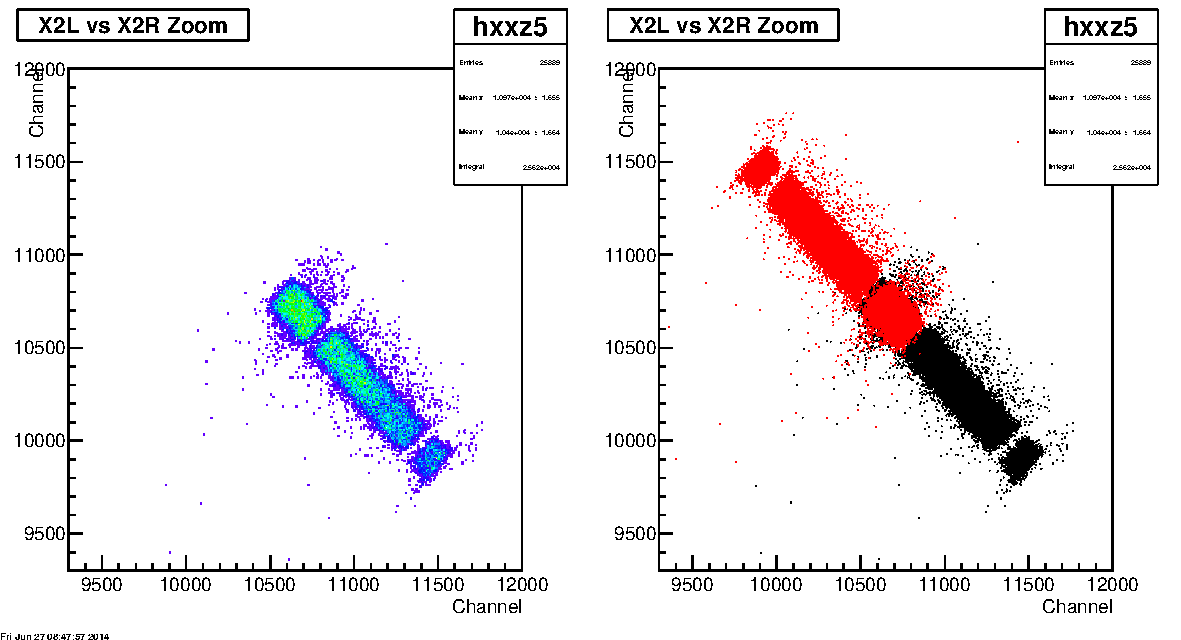
\includegraphics[width=\textwidth,keepaspectratio]{run00480_hxx5_reflect}
\caption{(Left) A plot of the signal X2L versus X2R.  By inspection, the correlation coefficient is approximately $-1$. Recall that XL signals correspond to the right-hand side of the detector (as viewed by the beam).  With $x=0$ defined as the left-hand side of the detector (as viewed by the beam), XR corresponds to the ``far'' signal. (Right) The plot from the left (black) is reflected (red) over the line $y=x$ as a visual test of gain-matching.}
\label{reflect}
\end{figure}
However, since the entire range of the detector is not illuminated, the reflection method only gives an approximate verification of the fit.  More significantly, the low dynamic range of the position signals 
(%the position signals 
covering $<1,280$ out of 40,960 channels) makes them very sensitive to the scaling parameter \verb|hxxcal[i][1]|.  Changes of 0.1\% in the scaling parameter will change the overlap of the reflected signals by several percent.  Therefore, a more sensitive calibration verification procedure is needed.
\subsection{Position Calibration}
\subsubsection{Method}
The relative positions of the features of the projection of the calibration mask are shown in Table~\ref{cal}.  What remains to be determined is the linear offset these features in terms of the relative position calculated using Eq.~\ref{detector_X}.  In order to determine the linear offset, and thus determine the calibrated detector position, the relative position of the gaps in the position spectrum need to be determined.  This is accomplished by fitting the position histogram with a piecewise-defined function.

\paragraph{Fitting the Peaks}
Traditionally, position calibration is accomplished by fitting known peaks in a spectrum.  In this test, the position spectra did not have peaks; rather they had wide regions illuminated by the scattered beam.  In order to attempt to fit these ``peaks,'' a nonconventional method was developed.
\vspace{0.5\baselineskip}
\par\noindent
\begin{minipage}{\linewidth}
\singlespace
\begin{lstlisting}
void lsload(Char_t *filename="cal/X1.lst")
{
  loadcal(filename);   
  ls1 = new TF1("ls1","([8]+[9]*x+[10]*x*x)*(x>(([0]-[7])/[6]))*(x<(([1]-[7])/[6]))+([8]+[9]*x+[10]*x*x)*(x>(([2]-[7])/[6]))*(x<(([3]-[7])/[6]))+([8]+[9]*x+[10]*x*x)*(x>(([4]-[7])/[6]))*(x<(([5]-[7])/[6]))");
  ls1->SetParName(6,"p6 range slope");
  ls1->SetParName(7,"p7 range offset");
  ls1->SetParName(8,"p8 fit offset");
  ls1->SetParName(9,"p9 fit slope");
  for(int i=0;i<6;i++){
    ls1->FixParameter(i,positions[i]);
    printf("i=%d positions[%d]=%5.1f parameter[%d]=%5.1f\n",i,i,positions[i],i,ls1->GetParameter(i));
  }
}  
\end{lstlisting}%
%\vspace{-1.0\baselineskip}
\end{minipage}
The function given in the code block above defines a polynomial over three ranges.  These three ranges correspond to the three ranges illuminated on each detector plane.  The quadratic function is explicitly defined in the \texttt{TF1} declaration as
\begin{equation}
\texttt{([8]+[9]*x+[10]*x*x)}
\label{eq:poly}
\end{equation}
instead of using the built-in ROOT function \verb|pol2| in order to force the fit parameters to be the same over each range.  This way, one function is fit to all of  the histogram data.  For calibrating the $x$-direction, the functional form of the Rutherford scattering cross section
\begin{equation}
\texttt{([8]+[9]*TMath::Power(sin([10]*x-[11]),-4))}
\label{eq:ruth}
\end{equation}
could also be used; however, the determination of the fit parameters using this equation are much less robust in ROOT as compared to fitting a histogram with a quadratic equation.  Furthermore, this form of the Rutherford scattering cross section only applies to $\varphi=0$.  Continuing with the quadratic fit, the range of the function may be defined in ROOT using the \texttt{TF1} constructor or it may be defined explicitly in the functional form.  In the above code block this is accomplished with the inclusion of the code segment \verb|*(x>a)*(x<b)| after each function definition.

By defining the function in this way, the range of the function may be an adjustable parameter.  The first six parameters of the function, which enter into the function via the range definitions, correspond to the calibration parameters shown in Table~\ref{cal}.  In the above code block, the calibration parameters are read in with the function \texttt{loadcal()} and then are made fixed in the \texttt{for} loop.  Parameters \texttt{[6]} and \texttt{[7]} are then the global slope and offset, respectively, of the known calibration parameters.  To aid in the fit, the variable parameters of the quadratic fit function (\texttt{[8]}, \texttt{[9]}, and \texttt{[10]}) can be measured on the central region only and then fixed.

The results of this technique are shown in Fig.~\ref{hxc_ls}.  This method is extremely sensitive to the initial values of the input parameters and is therefore both unreliable and ineffective. It also assumes \textit{a priori} knowledge of the position of the beam spot. In order to provide adequate input parameters for the fit, a robust and precise method was developed to locate the edges of the two ``valleys'' corresponding to the strips in the mask.

Figs.~\ref{hxc_ls} and \ref{hxc} are generated with a commands similar to the following.
\vsetroot
\begin{quote}
\begin{Verbatim}[firstnumber=0]
qfitc2mls("hxc2",87,141,3,"cal/X2.cal")
qfitc2mr("hxc2",87,141,3,"cal/X2.cal")
qfitc2mr("hxc3",13.1,40.8,3,"cal/Y2.cal")
\end{Verbatim}
\end{quote}
\vsetnone

\begin{figure}
\centering
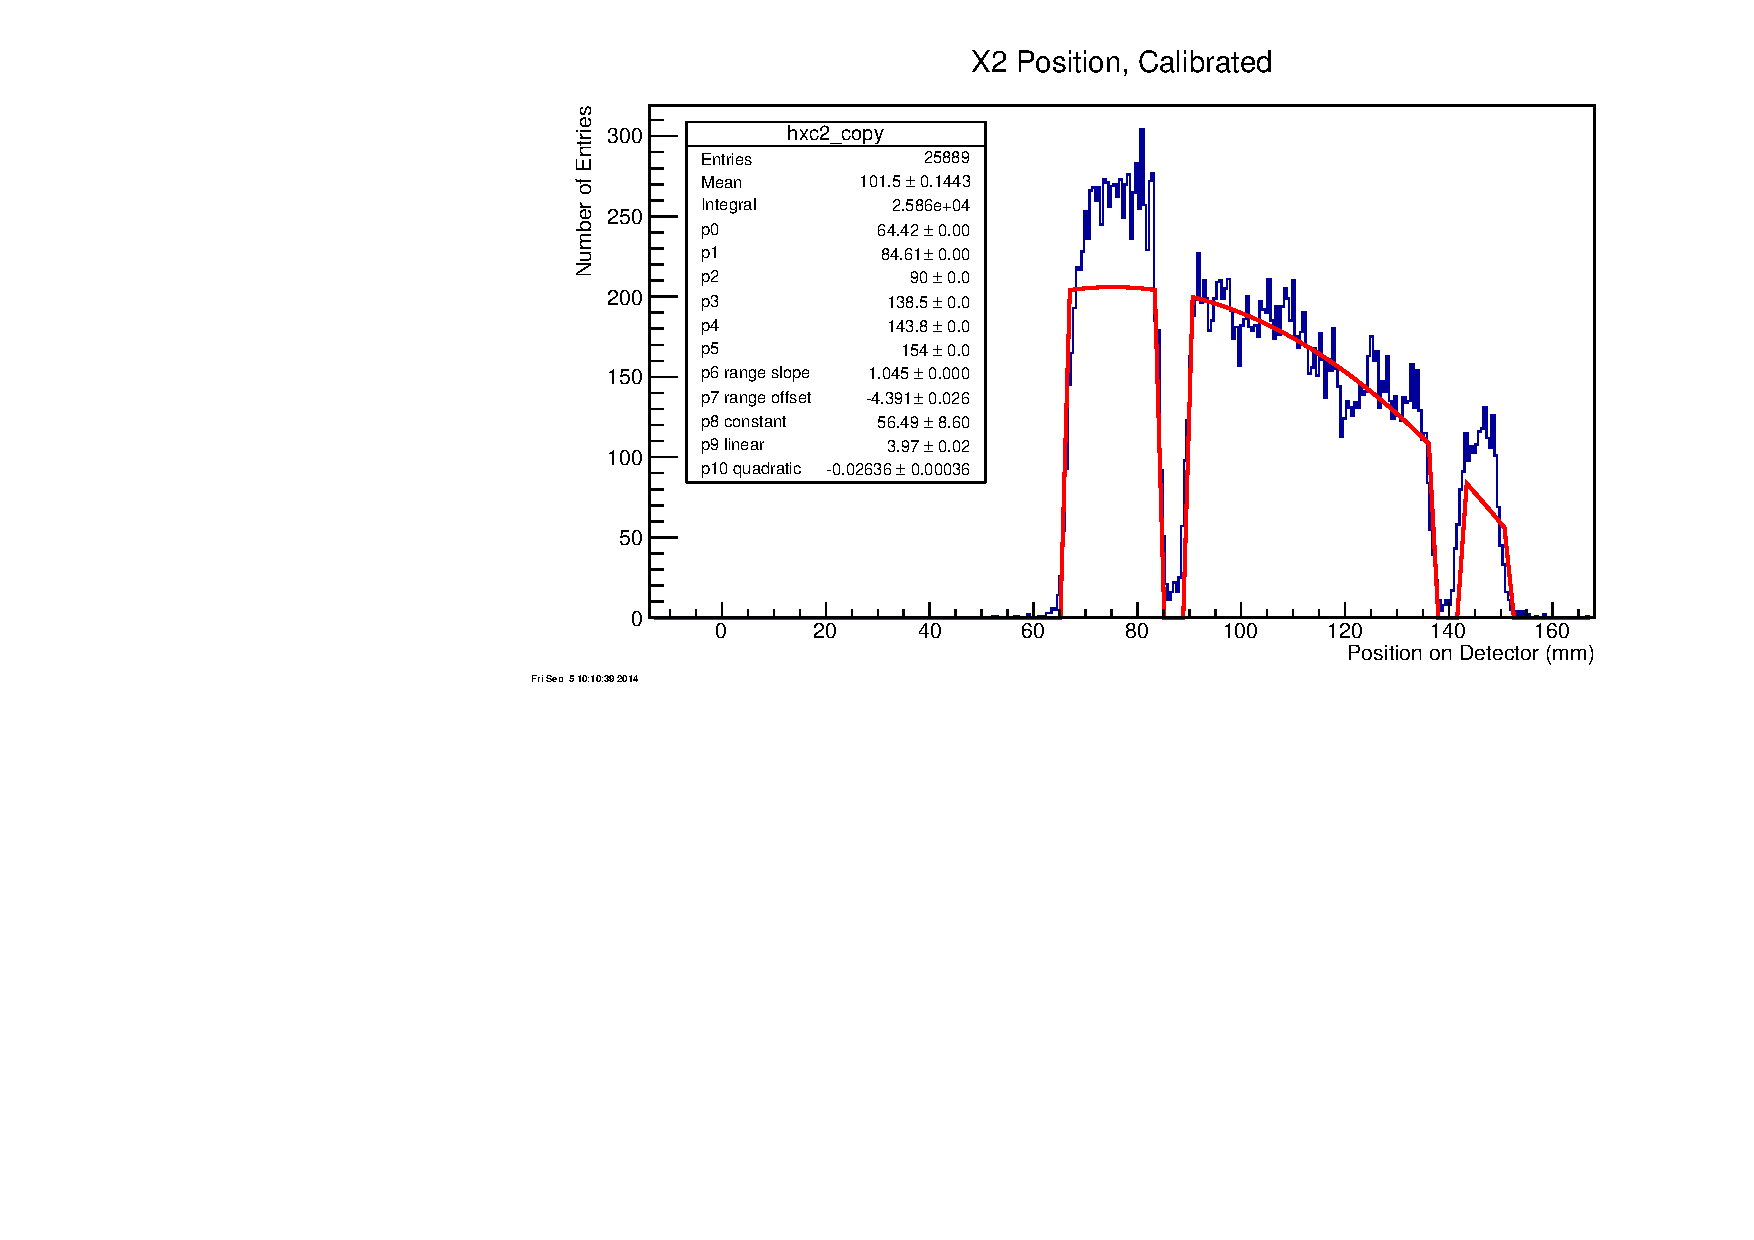
\includegraphics[width=\textwidth, keepaspectratio]{run_480_hxc2_ls}
\caption{Result of the fitting process by which the illuminated regions of the detector are fit.  The fixed relative positions of the edges of the illuminated region are fit to the ``peaks'' in the spectrum.}
\label{hxc_ls}
\end{figure}

\paragraph{Fitting the Valleys}
%Fitting the wide ``peaks'' in the spectrum is not very effective.  
Tables \ref{xpos} and \ref{ypos} provide 6 parameters with which to calibrate each of the the position spectra.  Including the outer edges of the illuminated region of the detector in the calibration procedure are dubious because the outer edges of the illuminated region are not sharply defined.  This is due to two effects.  First, the Kapton shields produce partial charge collection for trajectories at the edge of the detector.  This effect applies to both outer edges of the $y$-position spectra and the right-hand edge of the $x$-position spectra.  The second effect applies to the right-hand side of the $x$-position spectra.  This edge corresponds to the circular aperture of the mask, which does not provide a sharp cuttoff.

%Furthermore,
In addition to the uncertainty introduced by the edge effects outline above, the precise position of the outermost edges of the calibration spectra are not known \textit{a priori}. The parameters calculated in Tables \ref{xpos} and \ref{ypos} assume a point-like beam spot centered on the $z$-axis.  If the position of the beam spot is varied, the projected position of the mask will vary.  However, given that the $z$-position of the target, mask, and detector planes are fixed, the size and spacing of the gaps projected by the the vertical and horizontal strips of the mask are constant (at any given plane along the $z$-axis).

With these considerations in mind, the useful calibration parameters are limited to the central four edges.  By locating the center of each valley in the spectra, the relative position of all four calibration parameters can be determined with two fits. % (one for each valley). 
 This process is illustrated in Fig.~\ref{hxc}.  The data are scaled using the difference in the positions of the center of the gaps.  The scale factor is equal to the ratio of the known difference to  the measured difference. 
\begin{figure}
\centering
\hspace{\fill}
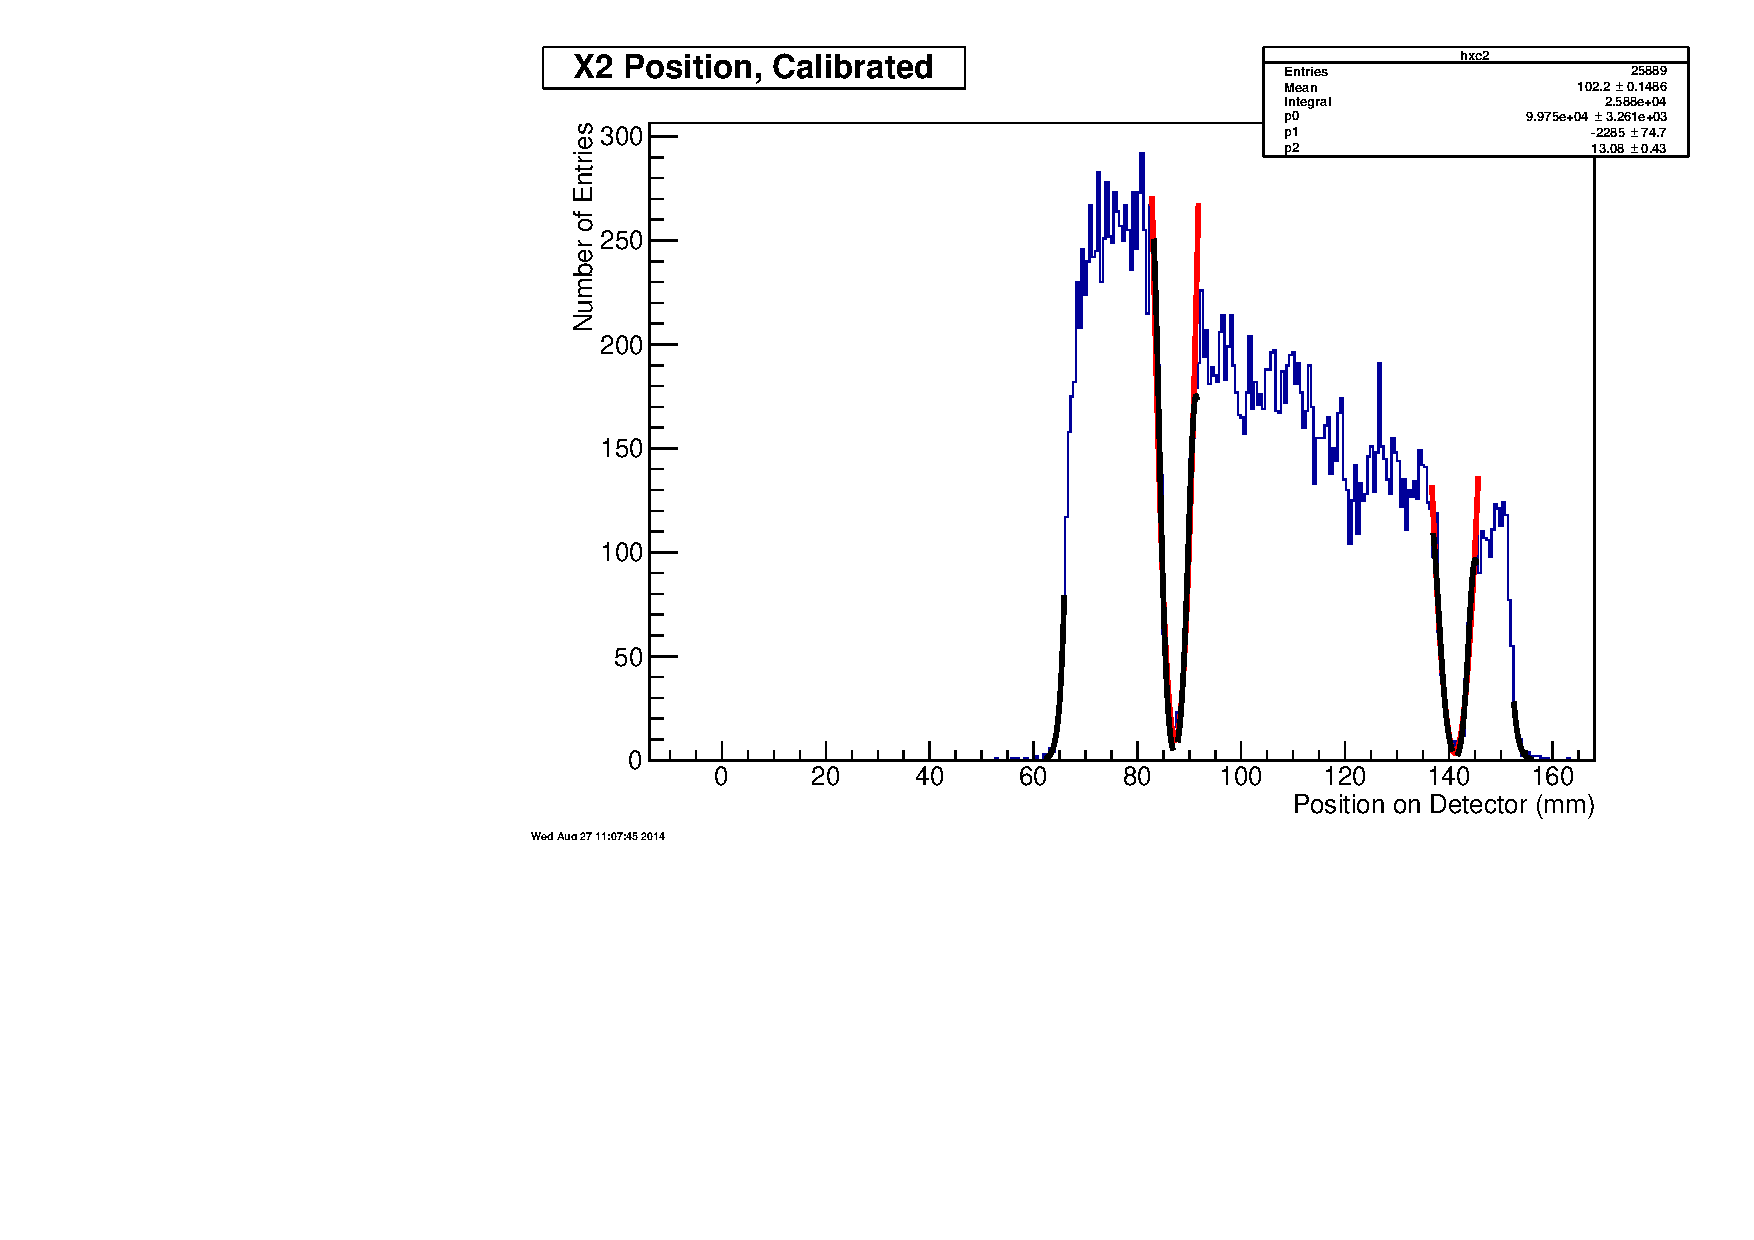
\includegraphics[width=0.48\textwidth, keepaspectratio]{run_480_hxc2}\hspace{\fill}
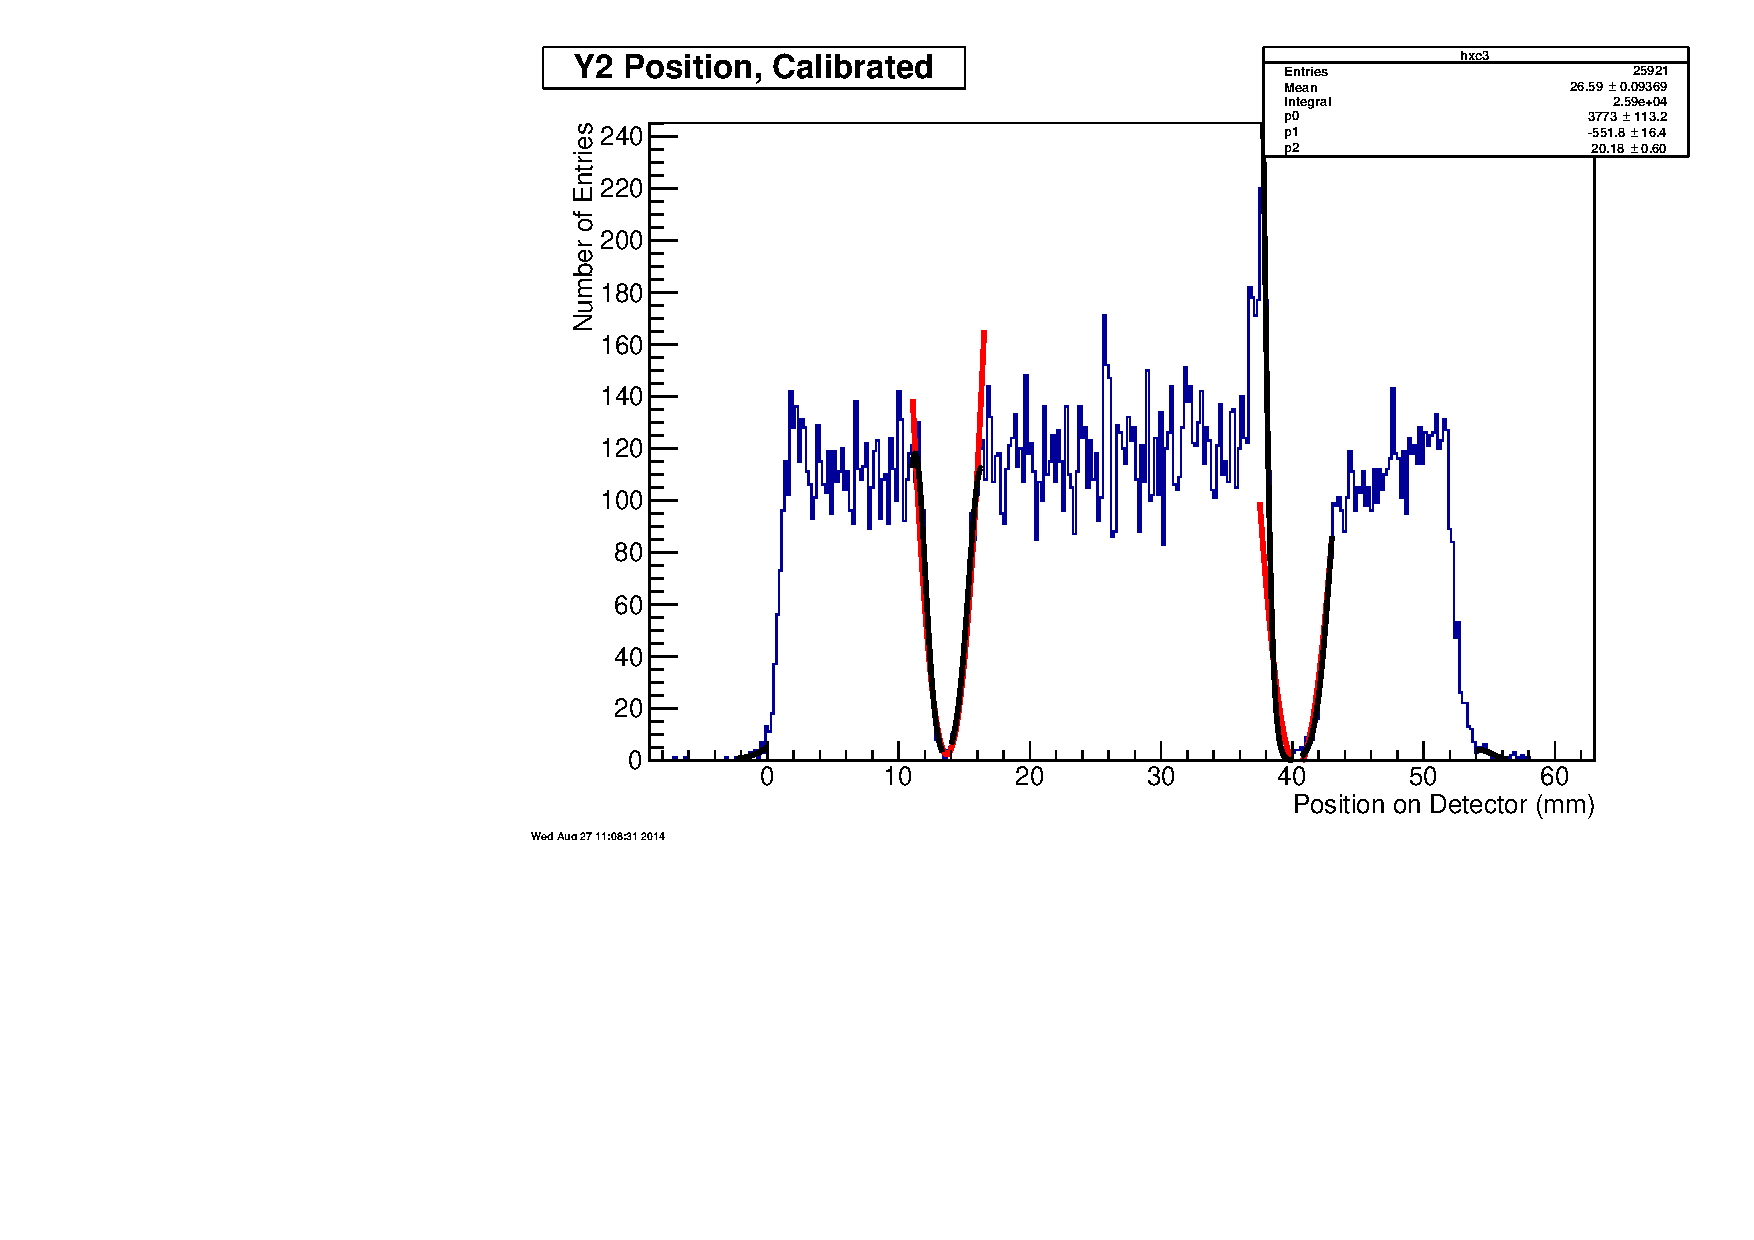
\includegraphics[width=0.48\textwidth, keepaspectratio]{run_480_hxc3} \hspace{\fill}
\caption{Position calibration technique.  Position X2 is shown on the left and position Y2 is shown on the right. The valleys between the illuminated areas of the detector are each fit with quadratic function (red lines) to locate the center of the gap.  The edges of the spectra are fit with gaussian functions (black lines) to determine the position resolution.}
\label{hxc}
\end{figure}

With this procedure, the position spectra are calibrated (in mm) based on the known detector geometry and independently of the $(x,y)$ position of the beam spot.  If the position of the beam spot is off-center, the position spectra are calibrated absolutely by the addition of a linear offset to correctly position the outer edges of the detector.  In the $y$-direction, this corresponds to centering the position spectrum. Fig.~\ref{yposreflect} shows the calibrated $y$-position spectra reflected with a given offset to align the edges.
\begin{figure}
  \centering
  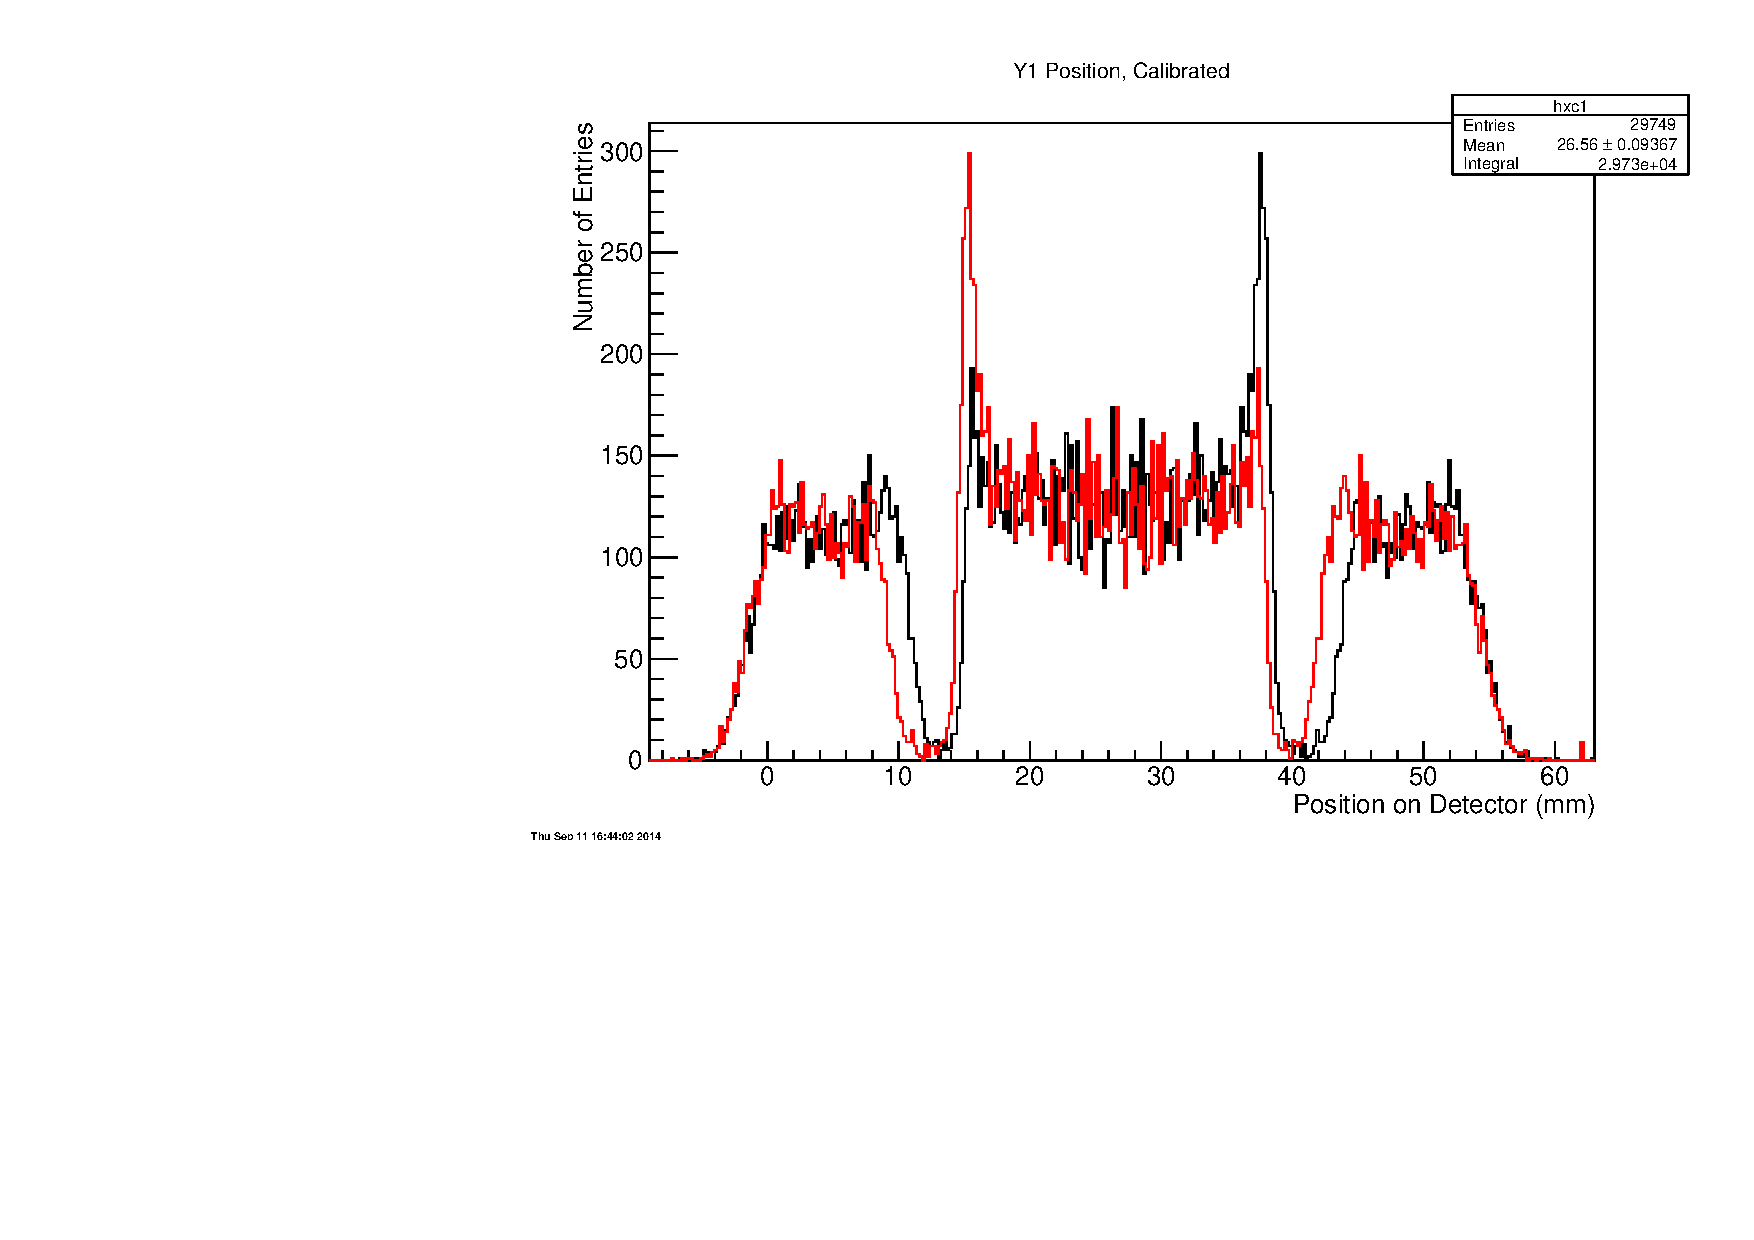
\includegraphics[width=0.48\textwidth,keepaspectratio]{run_480_hxc1_reflect}\hspace{\fill}
  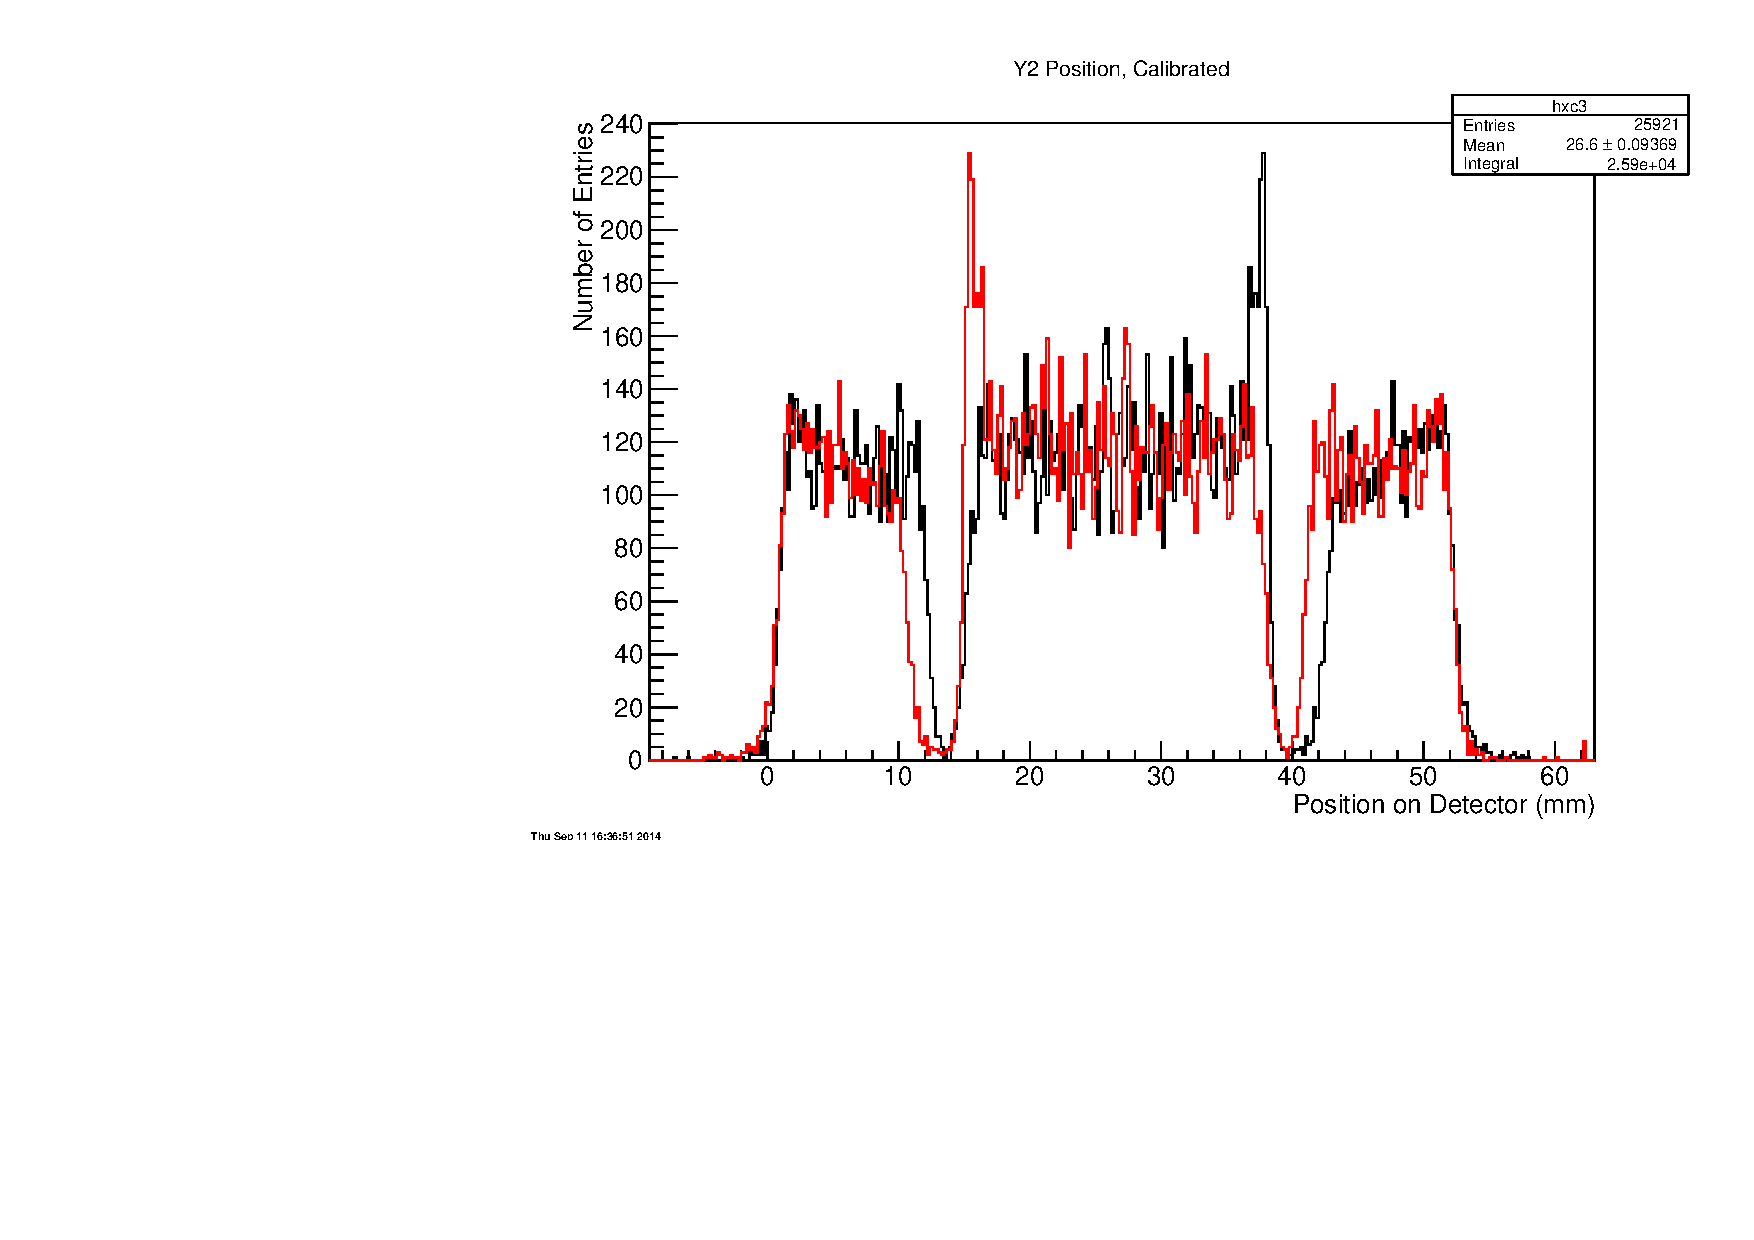
\includegraphics[width=0.48\textwidth,keepaspectratio]{run_480_hxc3_reflect}
   \caption{Calibrated $y$-position spectra (black) for each detector. The spectra have been reflected about the center of the detector and shifted (red) to align the outer edges of the spectra.  The Y1 spectrum has been shifted by 1.0\,mm and the Y2 spectrum has been shifted by 0.8\,mm.}
   \label{yposreflect}
\end{figure}
 %Calibrating the position spectra in this way provide a relative c
\subsubsection{Results}
The results of the valley fitting calibration procedure are shown for the $x$-positions in Fig.~\ref{htxc_x}.
\begin{figure}
\centering
\hspace{\fill}
\includegraphics[width=0.48\textwidth, keepaspectratio]{run_480_htxc1}\hspace{\fill}
\includegraphics[width=0.48\textwidth, keepaspectratio]{run_480_htxc7} \hspace{\fill}
\caption{Difference in anode channel (time) plotted against calibrated $x$-position. The dashed lines indicate the edges of the detector.  The solid lines indicate the edges of the Kapton shields, corresponding to the edges of the fiducial area.  The dot-dashed lines indicate the projected position of the mask.  The cutoff in data at the right-hand side of X2 does not coincide with the edge of the fiducial area of the detector.  This may be due interference from the edge of the Mylar window (cf. Fig.~\ref{rays})}
\label{htxc_x}
\end{figure}
In order to determine the position resolution, the width of a known feature must be measured.  Usually this is done by measuring with width of peaks in spectra.  However, lacking any peaks, the edges in  the spectra can be used in similar manner.  The sharpness of the central edges of the position spectra provides a means by which to determine the position resolution.  The results of such an analysis are shown in Table~\ref{pos_res}.
\begin{table}[ht!]%
\centering
\begin{tabular}{c..}
\hline
\multicolumn{1}{c}{Edge}&\multicolumn{1}{c}{$\sigma$ (mm)}&\multicolumn{1}{c}{FWHM (mm)}\\ \hline \hline
%Edge & 3.974 & FWHM\\
1 & 1.43&3.36\\
2 & 1.48&3.49\\
3 & 1.68&3.95\\
4 & 1.19&2.79\\
Average & 1.44&3.40\\
\hline
\end{tabular}
\caption{Calibrated position resolution for position X2.}
\label{pos_res}
\end{table}
The resolutions presented in Table~\ref{pos_res} represent the cumulative effect of multiple contributions. Some of the possible contributions to the total measured position resolution are as follows.
\begin{itemize}
  \setlength{\itemsep}{0pt}
\setlength{\parskip}{0pt}
\setlength{\parsep}{0pt}
  \item The intrinsic detector resolution.
  \item The transverse extent of the particle trajectories.
  \item The position, extent, and distribution of the beam spot.
  \item The effect of beam scattering off of the mask.
\end{itemize}
%The transverse extent of the particle trajectories tend to smear out the position. In addition to the intrinsic detector resolution,
In order to determine the intrinsic position resolution of the detectors the other contributions to the measured resolution need to be deconvoluted.  The is accomplished with simulations.
\subsection{Simulations}
A Monte Carlo simulation has been constructed to study the various contributions to the measured resolution.  An example output is shown in Fig.~\ref{sims}. To produce the figures discussed in this section, the simulation included a uniform spherical scattering distribution and a finite beam spot.  Specifically, the beam spot has been simulated as a symmetric Gaussian distribution with 90\% of the beam falling within a radius of $\rho=1.0$\,mm ($\sigma = 0.608$\,mm). This beam spot size was selected to be conservatively large and yet physically reasonable.
\subsubsection{Contributions}
One of the purposes of studying the detector via a simulation was to deconvolve the various contributions to the detector resolution. The results of the simulation study indicate that the observed detector resolution is dominated by the intrinsic detector resolution.  As discussed in Section~\ref{cal_def}, the contribution of the transverse extent of particle trajectories is less than 170\,$\mu$m at the edges of the detector. Near the center of the detector, the contribution approaches zero. These effects are neglected in all of the simulations.

To isolate the contribution of the beam spot size, simulations were run neglecting the effects of beam scattering and detector resolution. Fig.~\ref{sims} shows the simulated position spectra from detector 2.  Comparing Fig.~\ref{sims} with Fig.~\ref{hxc}, one sees that the beam spot size has a minimal contribution to the measured detector resolution. This is not surprising given the distance between the target and the detectors (682.9\,mm) and reasonably-assumed size of the beam spot (1--2\,mm). In order to reproduce the observed resolution in Fig.~\ref{hxc} from the contribution of the beam spot alone, physically unrealistic beam spot sizes are required. For example, a beam spot greater than the size of the target foil is required.
\begin{figure}%
\includegraphics[width=\columnwidth]{sims}%
\caption{Simulated positions spectra of detector 2.}%
\label{sims}%
\end{figure}

\subsubsection{Fitting the Data}
The determination of the detector resolution is accomplished by fitting the data with the simulation. The position of the beam spot is accounted for by geometrically aligning the features of the simulation with those the data. Once the simulation is aligned to the data, the measurement resolution of the simulation is varied to match the shape of the data. Fig.~\ref{sim_comp} show the result of fitting the data with the simulation in order to determine the position resolution of the detector. Because the simulation adequately reproduces the data without including edge scattering, implementation of that effect is neglected. In this example, the data was best fit with a simulated intrinsic detector resolution of 1.3\,mm (3.06\,mm~FWHM).  This fit is consistent with the dubious edge-fitting method presenting in the previous section. For an example such as this, where the wires are not resolved, the quality of the fit of the simulation could be improved on the order of 8\% by including a realistic angular distribution.
\begin{figure}%
\includegraphics[width=\columnwidth]{run_480_compX}%
\caption{Simulated and measured $x$-position spectra of for each detector. The data (blue) have been fit with a simulated spectra using the following assumptions: a 1.43\,mm~FWHM beam spot centered at the origin and a detector resolution of 1.3\,mm (3.06\,mm~FWHM).}%
\label{sim_comp}%
\end{figure}





%\input{src/time_stamp}

\end{document}  
